% Root File for a UC Dissertation / Thesis
% UCD thesis class: c/o Shwaine <shwaine@shwaine.com>
%
% modified by Dylan Beaudette, 2006,2010
% modified  and source uploaded to github by Alex Mandel, 2014
% Source code available at http://github.com/wildintellect/ucdthesis
\documentclass[12pt,oneside,draft]{ucdthesis}
%\documentclass[10pt,twoside,final]{ucdthesis}
% \documentclass[10pt,oneside,final]{ucdthesis}

\usepackage[final]{graphicx}
% TODO: this makes strange things happen in the header...
% this is the version that grad studies wants
% \documentclass[11pt,oneside,final]{ucdthesis}

% when we are giving people drafts, use more of the page:
\usepackage[letterpaper,
    inner=1.0in,
    outer=2.25in,
    top=1.25in,
    bottom=2.0in,
    marginparsep=0.25in,
    marginparwidth=1.0in]{geometry}

\setlength{\footskip}{1.25in}
\setlength{\headsep}{1.25in}
\setlength{\headheight}{15pt}
% need this for the \foreach command
\usepackage{tikz}
\usetikzlibrary{calc,shapes,arrows,positioning}

% Turn on single spacing with \ssp.
% Turn on double spacing with \dsp.
% By default, your dissertation is double spaced, as is required by UCD.
\usepackage{setspace}
\makeatletter
\let\@currsize\normalsize
\makeatother
\setstretch{1.86}

% spacing in figures and tables and their captions can be
% changed here (\ssp for single-space, empty for same as surrounding
% text); for this to work, the command \figsp has to be included
% in every figure and table right after the \begin{figure}
% \def\figsp{\ssp}
%\def\figsp{}


% useful for drafts
% line numbers:
% http://www.ctan.org/tex-archive/help/Catalogue/entries/lineno.html
%
%\usepackage{lineno}

%
% SVN integration
%
% \usepackage{svnkw}

\usepackage{calc}

% customized headers
%
% http://www.ctan.org/tex-archive/help/Catalogue/entries/fancyhdr.html
\usepackage{fancyhdr}

\newlength{\myoddoffset}
\setlength{\myoddoffset}{\marginparwidth + \marginparsep}

\rhead{\input{git-header}}
\chead{\textbf{---DRAFT---}}
\lhead{}
\cfoot{---\thepage---}
\fancyheadoffset[R]{\myoddoffset}
\fancyfootoffset[R]{\myoddoffset}

\fancypagestyle{plain}{%
    \fancyhf{}
    \fancyfoot[C]{---\thepage---}
    \fancyhead[C]{\textbf{---DRAFT---}}
    \fancyhead[R]{\input{git-header}}
\fancyheadoffset[R]{\myoddoffset}
\fancyfootoffset[R]{\myoddoffset}
}
\fancypagestyle{frontmatterstyle}{%
    \fancyhf{}
    \fancyfoot[C]{---\thepage---}
    \fancyhead[C]{\textbf{---DRAFT---}}
    \fancyhead[R]{\input{git-header}}
\fancyheadoffset[R]{\myoddoffset}
\fancyfootoffset[R]{\myoddoffset}
}

% a better verbatim environment: c/o Pete Dirac
% use like this:
%   \begin{Verbatim}[fontsize=8]
%       foobar
%    \end{Verbatim}
% \usepackage{fancyvrb}


% more flexible math support
\usepackage{amsmath}

% allow some pages to be landscape
\usepackage{lscape}

% more flexible definition of table environments
\usepackage{ctable}

%need this for \includegraphics{}
\usepackage{graphicx}

%enable the listings package specifically for including programming code
\usepackage{listings}

%Special hack to make code listings not break pages, fyi they must be short then
\usepackage{float}
\floatstyle{plain} % optionally change the style of the new float
\newfloat{Code}{H}{myc}

%test alternative to listings package minted which requires the python pygments package
%minted was installed to latex by hand
%\usepackage{minted}

% TODO: use the new subfig package instead
% http://www.ctan.org/tex-archive/macros/latex/contrib/subfig/
%
%use this to put figures side by side
\usepackage{subcaption}

 % PDF links --- > breaks with some bibliography entries
% \usepackage{hyperref}

% nice looking, parenthetical references
%\usepackage[sorting=nyt,natbib=true,citestyle=authoryear,bibstyle=authoryear,maxnames=3,refsection=chapter]{biblatex}
%\usepackage[sorting=nyt,natbib=true,citestyle=authoryear,bibstyle=authoryear,maxnames=3,refsection=chapter]{biblatex}

\usepackage[utf8]{inputenc}
\usepackage[english]{babel}

\usepackage{natbib}
\renewcommand\bibname{References}
\def\newblock{\hskip .11em plus.33em minus.07em}
\bibliographystyle{abbrvnat}
\setcitestyle{authoryear, open={(},close={)}}
%%\usepackage{chapterbib} % incompatible with biblatex
%\bibliography{dissertation}
%\defbibheading{bibliography}{%
%	\section{References}
%	}
%	
%% bibliography can be single-spaced for UC thesis format
%\appto{\bibsetup}{\ssp}
%	

\usepackage{textcomp}% for '\textdegree' macro

%make the index
% \usepackage{makeidx}
% \makeindex

% custom colors
\usepackage{color}
% make a color for comments
\definecolor{MyDarkBlue}{rgb}{0,0.08,0.45}

% customized captions with bold label and small, italic text
% table captions are located above tables
% http://www.kronto.org/thesis/tips/custom-captions.html
% http://www.ctan.org/tex-archive/macros/latex/contrib/caption/
% does this have any effect?
%\usepackage{caption}
% \renewcommand{\captionfont}{\small\itshape}
%
\usepackage[hypcap,font=singlespacing]{caption}
%\usepackage{subcaption}
% modern method for setting up captions\
\captionsetup{margin=10pt,font=small,labelfont=bf}
%
% fix so that table captions have correct spacing
\captionsetup[table]{position=top}



% %
% %  fit more material on the page:
% %
%
% reset some float-controlling parameters
\renewcommand{\floatpagefraction}{0.8}	% require fuller float pages

% N.B.: floatpagefraction MUST be less than topfraction !!
\renewcommand{\topfraction}{0.9}	% max fraction of floats at top
\renewcommand{\bottomfraction}{0.8}	% max fraction of floats at bottom


% PDF formatting options, indexing, hyperlinking, with control over link style
%Set PDF Metadata
\title{The Effects of Concurrent Bandwidth Feedback on Robotics Manual Control Tasks}
\author{John A. Karasinski}
\makeatletter
\usepackage[pdftex,
            pdfauthor={\@author},
            pdftitle={\@title},
            %pdfsubject={Subject},
            %pdfkeywords={Comma, List, Keywords},
            %pdfproducer={Latex with hyperref, or other system},
            %pdfcreator={pdflatex, or other tool}
            ]{hyperref}
\makeatother
\hypersetup{
    % driver=pdftex,
    final=true,
	colorlinks=true,
	urlcolor=blue,
	linkcolor=blue,          % color of internal links
    citecolor=blue,        % color of links to bibliography
    filecolor=magenta
}

%Use an additional package to make bookmarks point to the top to tables, figures and listings
\usepackage[all]{hypcap}

%Alex's customizations
\usepackage{indentfirst} %Indents first paragraph of chapter
\usepackage{datatool} %Allows import of csv and other data-tables
\usepackage{varwidth}
\usepackage{color}
\usepackage{rotating}
%\AtEveryBibitem{\clearfield{month}} %Cleaner references without month being printed

\graphicspath{{./figures/}{./plots/}}

\newcommand{\tablepath}{./tables/}

\makeatletter
\newcommand{\includetable}[1]{%
  \@ifundefined{tablepath}{%
    \InputIfFileExists{#1}{}{}%
  }{%
    \InputIfFileExists{\tablepath/#1}{}{\InputIfFileExists{#1}{}{}}%
  }
}
\makeatother

\usepackage{booktabs}
\usepackage{dcolumn}
\newcolumntype{.}{D{.}{.}{-1}}
% more space between table rows
\renewcommand{\arraystretch}{1.2}

\usepackage{csquotes}
\renewcommand\mkbegdispquote[2]{\leavevmode\llap{``}}
\renewcommand\mkenddispquote[2]{#1''#2}

\usepackage{todonotes}
\newcommand{\tinytodo}[1]
{\todo[size=\small]{\linespread{1.0}%
\selectfont%
#1%
\par
}}

\usepackage{mathtools}

\usepackage{enumitem}

\usepackage{multirow}

\usepackage{makecell}

\usepackage{nameref}

\usepackage{siunitx}
\DeclareSIUnit\inch{in}
\DeclareSIUnit\feet{ft}
\DeclareSIUnit\foot{ft}
\DeclareSIUnit\bps{bps}
\DeclareSIUnit\bits{bits}

\hyphenation{NASA-TLX}

%\usepackage[maxfloats=58]{morefloats}

\renewcommand\bibname{References}

\usepackage{flexisym}

\newcolumntype{C}[1]{>{\centering\let\newline\\\arraybackslash\hspace{0pt}}m{#1}}

\newcommand{\PreserveBackslash}[1]{\let\temp=\\#1\let\\=\temp}
\newcolumntype{R}[1]{>{\PreserveBackslash\raggedleft}p{#1}}
\newcolumntype{L}[1]{>{\PreserveBackslash\raggedright}p{#1}}

\usepackage{pifont}
\usepackage{newunicodechar}
\newunicodechar{✓}{\ding{51}}
\newunicodechar{✗}{\ding{55}}

\usepackage{adjustbox}
\usepackage[framemethod=tikz]{mdframed}

%%% Document Portion:
\begin{document}


%
%% Title, Front Matter, and Abstract:
% Skip for draft
% % Declarations for Front Matter
\title{Concurrent Bandwidth Feedback for Complex Manual Control Tasks}
\author{John A. Karasinski}

% Choices are September, December, March, June
\degreemonth{June}
\degreeyear{2020}

\committee{Stephen K. Robinson}{Ron A. Hess}{Zhaodan Kong}{}{}

%Your Graduate Group
\officialmajor{Mechanical and Aerospace Engineering}
\graduateprogram{Mechanical and Aerospace Engineering}

%%%%%%%%%%%%%%%%%%%%%%%%%%%%%%%%%%%%%%%%%%%%%%%%%%%%%%%%%%%%%%%%%%%%%%%%
\abstract{Abstract.}

\acknowledgments{
  Thank you to my fellow Human/Robotics/Vehicle Integration and Performance Lab members, who elevated this work with their high standards.
  Thank you to Professor Robinson, who provided the inspiration for this project and has guided me throughout the whole process.
  Thank you to my committee members, Professor Hess and Professor Kong, who provided support in shaping the research.
  Thank you to Richard Joyce and Sarah O'Meara, who were always willing to discuss research over coffee.\\
  \\
  Thank you to the San Jose State University Research Foundation, who provided financial support.
  Thank you to the Link Foundation, who selected me for the Advanced Training and Simulation Fellowship and provided financial support.
  Thank you to NASA Ames Research Center's Human Systems Integration Divison for having me as a Pathways Intern, providing financial support, and the knowledge and expertise of your wonderful staff.\\
  \\
  Thank you to the subjects who volunteered their time and made this research possible.\\
  \\
  Thank you to my family, without whom I would, quite literally, not be here.
}


%
% the chapters
%

% set page style:
% make the chapter and section smaller, chapter and section numbers are removed
% fancyplain will keep the page numbers at the bottom of all pages
%\pagestyle{fancyplain} %Note the \fancyplain command !!!
%\renewcommand{\chaptermark}[1]{\markboth{\small{#1}}{}}
%\renewcommand{\sectionmark}[1]{\markright{\small{#1}}{}}

\pagestyle{fancy}

% TODO: this is only for draft copies !!
% start line number printing
%


\tableofcontents

\chapter{Introduction}

\section{Motivation}
\label{sec:intro_overview}
We aim to improve performance and decrease learning times for novice operators of highly complex motor control tasks.
We are specifically interested in modeling and improving human performance in flight tasks, which generally require extensive training to master.
The Federal Aviation Administration (FAA), for instance, requires a minimum of 1,500 hours as a pilot to captain a U.S. airline~\citep{FAA}.
Being able to decrease this training time could lead to significant savings in cost, and the predictive ability provided by modeling human performance allows for safer operation of the aircraft.

A variety of skills can be classified as motor control tasks, such as playing tuba, pole vaulting, or flying an aircraft.
An individual's performance in any of these skills can change dramatically as they transition from a novice to an expert through training.
We are interested in measuring and modeling this performance as it changes over the course of the training process.

Humans rely on several kinds of feedback during training to improve their performance in motor control tasks.
Feedback can be largely grouped into two types: internal, or intrinsic feedback, and external, or extrinsic feedback.
Intrinsic feedback is anything a person can infer using their senses: the feel of the valves of the tuba as you play, the sense of balance mid-jump, or the sound the aircraft engine makes during a climb.
Extrinsic feedback, conversely, is provided by an external source, often in the form of an expert instructor.
Extrinsic feedback comes in a variety of forms, and has a long history of improving performance in a large variety of motor control tasks.

We will focus on a specific type of extrinsic feedback, which is known as concurrent bandwidth feedback (CBF).
Concurrent feedback is provided in real-time, as an operator is completing a task.
Bandwidth feedback is provided when a objective particular value deviates outside a designated range or bandwidth.
Concurrent bandwidth feedback is, therefore, feedback provided to an operator in real-time when a signal deviates out of a predefined range.
This type of feedback has been shown to improve performance in many simple motor control tasks, but has not been investigated in complex, high degree of freedom tasks.

It is important to note that this feedback should be thought of as qualitative feedback, not as an additional form of quantitative guidance.
We are not interested in adding additional displays or gauges to control interfaces, but would prefer to modify existing indicators, during training, to better inform an operator as to how well they are performing a task.
Despite extensive evidence as to the effectiveness of this feedback, the mechanism by which performance is improved has yet to be explained, nor integrated into human performance models.
We will attempt to explain why this feedback is effective in enhancing learning and integrate this explanation into a model.

\section{Background}

\subsection{Augmented Feedback}
\subsection{Pilot Modeling}
\begin{figure}[tb]
    \begin{center}
        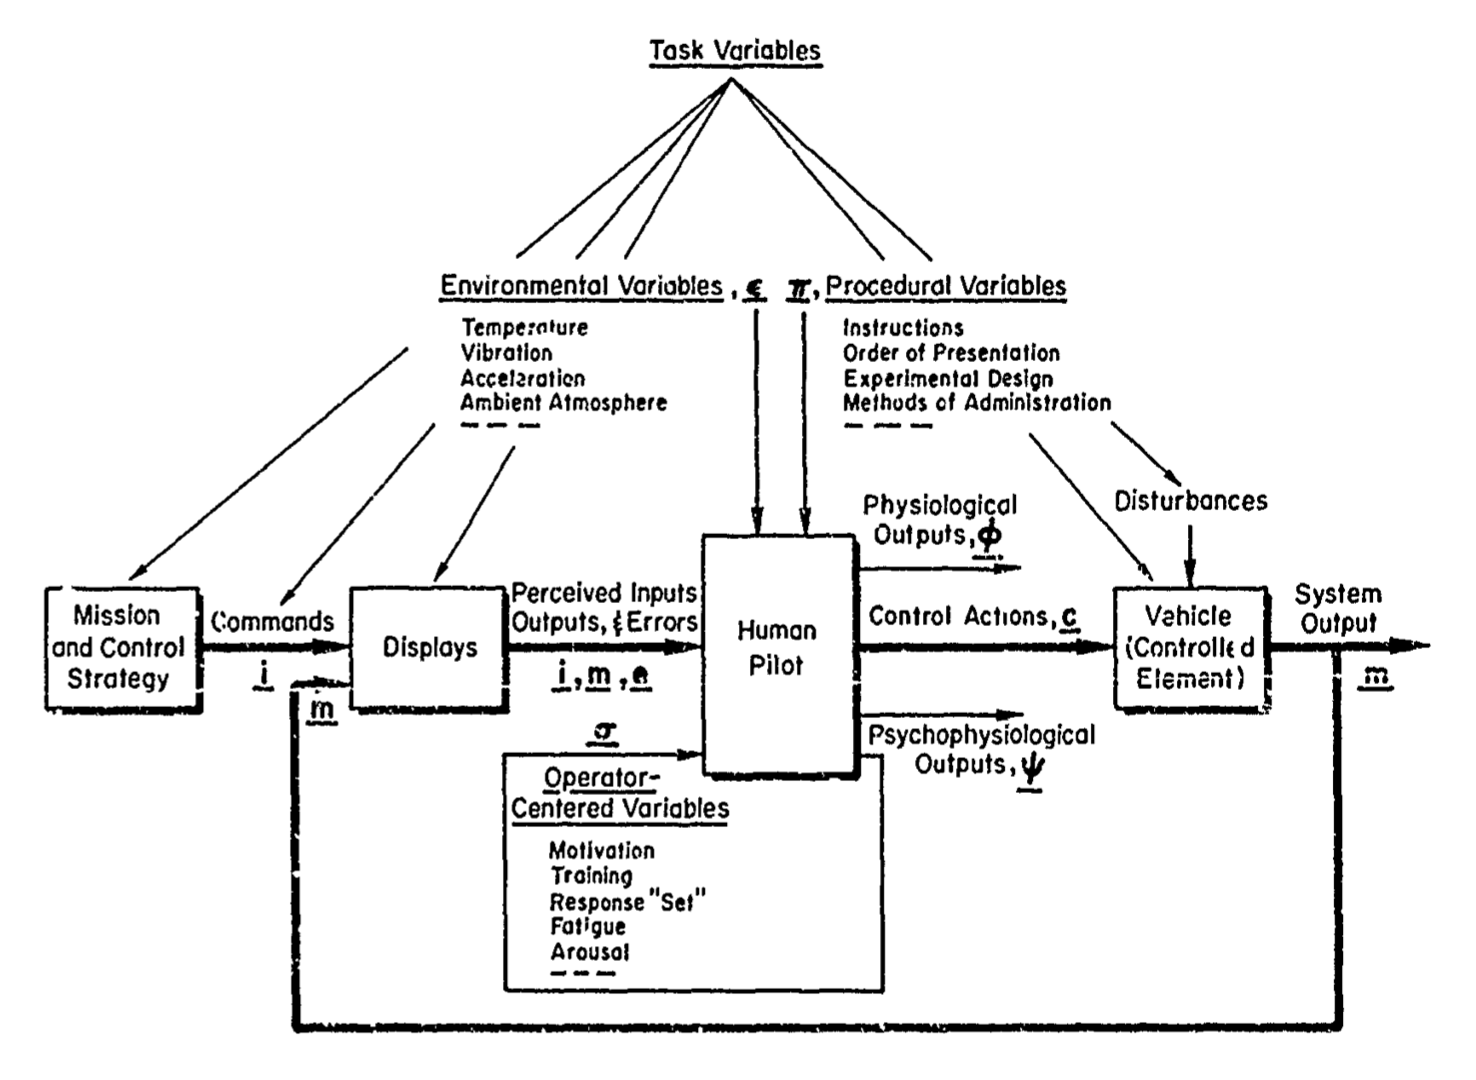
\includegraphics[width=0.8\linewidth]{figures/Introduction/Screen_Shot_2018-07-25_at_10_37_08_AM.png}
        \caption[Variables affecting the pilot/vehicle system]{Variables affecting the pilot/vehicle system, from~\citep{mcruer_mathematical_1974}.}
        \label{figure:mcruer1974}
    \end{center}
\end{figure}

In addition to popularizing the concept of feedback, the creation of control theory in the early 1940s also provided the tools required for the mathematical modeling of the human pilot.
At the time, new weapons were being created for World War 2 which could only be used effectively with trained operators working in tandem with the machine.
While it was thought that a human could be viewed as a unique kind of servomechanism in the control feedback loop, it was still unclear what factors affected human performance.
Early work by Tustin and others extended the control theory framework and applied these theories to actual human operators~\citep{tustin_investigation_nodate}.
Particular interest was focused on ``attempt[ing] to find the laws of relationship of movement and error. In particular, it was hoped that this relationship [would] be approximately linear and so permit well developed theory of `linear servomechanisms' to be applied to manual control in the same way as it applies to automatic following~\citep{tustin_investigation_nodate}.''
This would allow for the prediction of human performance and the ability to predict the limits of human control.

These early works were summarized in McRuer's 1957 report, ``Dynamic Response of Human Operators''~\citep{mcruer_dynamic_1957}.
This work evaluated measurements for single-input/single-output (SISO) manual control systems and developed predictive models consistent with this data.
Indeed, McRuer writes, ``[i]t is possible, without doing violence to the data, to obtain describing functions which are generally applicable to the results of the many diverse experiments~\citep{mcruer_dynamic_1957}.''
The report concludes by describing a hypothetical transfer function of the human operator which includes a time delay, a neuromuscular lag, and a gain.
McRuer's early model of the complete pilot/vehicle system is presented in Figure~\ref{figure:mcruer1974}.
McRuer revisited these results in 1974, after three decades of supporting engineering and experimental psychology experiments and was able to further generalize these results to a wide variety of system dynamics~\citep{mcruer_mathematical_1974}.
In his study, McRuer completed a detailed analysis which included the human response to proportional, rate/velocity, and acceleration type controlled element dynamics, see Table~\ref{table:mcruer1974a}.
The result of this report was the now famous ``crossover model,'' which relates the operator and controlled element transfer characteristics by the equation
\begin{align}
    Y_c(jw) Y_p(jw) = \dfrac{w_c e^{-jw \tau_e}}{jw}
\end{align}
where $Y_c$ is the controlled element transfer function, $Y_p$ is the approximate human operator transfer function, $w_c$ is the crossover frequency, and $\tau_e$ is the effective time delay of the pilot.
The crossover model is so named as it allows for linear behavior at approximately -20 dB/decade slope in the region of the crossover frequency.
The approximate human operator response to several controlled element transfer functions and their combined open-loop transfer function are presented in Table~\ref{table:mcruer1974b}.
Modeling the human pilot with the crossover enabled a more complete view of the complete pilot/vehicle system, and allowed for human factors recommendations towards the design of new vehicles.
Even today, the crossover model is used as the standard for describing pilot/vehicle systems at the crossover frequency~\citep{mcruer_human_1965, mcruer_mathematical_1974, xu_review_2017}.

\begin{table}[tb]
    \centering
    \includetable{intro-idealized-control-elements.tex}
    \caption[Example Applications of Idealized Controlled Element Forms]{Example Applications of Idealized Controlled Element Forms, adapted from~\citep{mcruer_mathematical_1974}.}
    \label{table:mcruer1974a}
\end{table}

\begin{table}[tb]
    \centering
    \includetable{intro-human-operator-characteristics.tex}
    \caption[Summary of Human Operator Approximate Characteristics]{Summary of Human Operator Approximate Characteristics, adapted from~\citep{mcruer_mathematical_1974}.}
    \label{table:mcruer1974b}
\end{table}

The continued demand for human pilot models for use in informing vehicle design, as well predicting, preventing, and explaining accidents has led to a variety of more complex pilot models since the creation of the crossover model.
A recent review by Xu et al. in 2017 surveyed the state of the art in human pilot modeling and grouped existing models into three classes of models based on: control theory, human physiology, and intelligence techniques~\citep{xu_review_2017}.
Classical models based on control theory include the McRuer crossover model and optimal control models by Kleinman et al. developed in the early 1970s~\citep{kleinman_optimal_1970, baron_optimal_1970}.
Of these three overarching sets of models, the models based on human physiology are of the greatest interest here.
Models based on human physiology were developed to understand human pilot perception and control behavior, and include the Hess structural model~\citep{hess_structural_1980, hess_model_1990, hess_unified_1997}, Hosman's descriptive model~\citep{hosman_pilots_nodate, hosman_pilots_1999}, and the biodynamic model~\citep{griffin_validation_2001}.
Recent intelligence models take advantage of techniques including fuzzy control and neural networks~\citep{zaychik_conspectus_2006, gestwa_modelling_2003}.

\begin{figure}[tb!]
    \begin{center}
        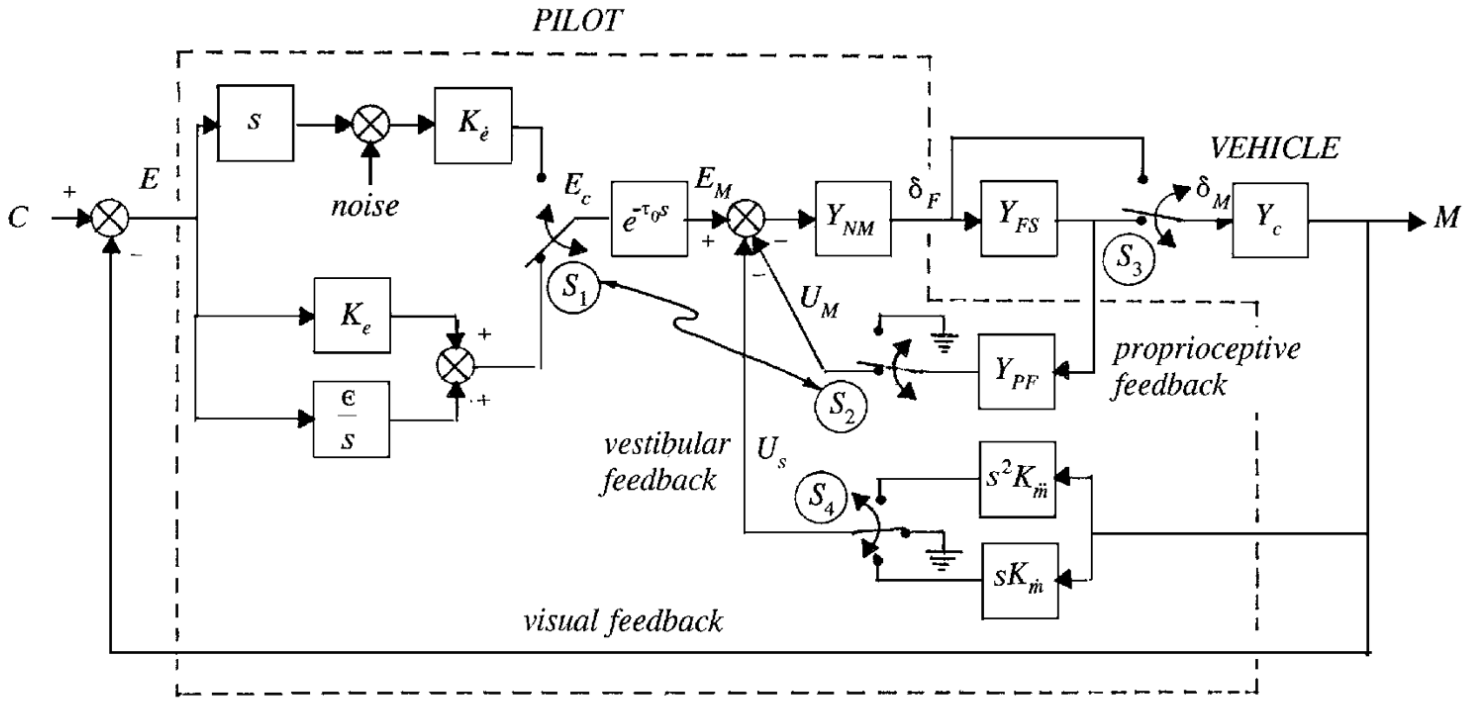
\includegraphics[width=0.8\linewidth]{figures/Introduction/Screen_Shot_2018-07-31_at_11_21_44_AM.png}
        \caption[The Hess Structural Model of the Human Pilot]{The Hess Structural Model of the Human Pilot, from~\citep{hess_unified_1997}.}
        \label{figure:structuralmodel}
    \end{center}
\end{figure}

While the McRuer was very successful in predicting pilot behavior, it it did not attempt ``to describe the underlying structure which contributes to human pilot dynamics~\citep{hess_structural_1980}.''
For this reason, the Hess Structural Model is of particular interest due to the incorporation of multiple sensory channels and models of visual acuity and the time-varying human pilot~\citep{hess_modeling_2009}.
The Structural Model includes the effects of the neuromuscular system, the force-feel characteristics of the input device, and the contributions of proprioceptive, vestibular, and visual feedback, see Figure~\ref{figure:structuralmodel}.
One of the key strengths of the Structural Model is the relatively few number of free parameters that need to be set to predict pilot performance.
The model has been used in predicting and evaluating handling qualities and pilot-induced oscillation rating levels for helicopters, Boeing 747, Lockheed C-5A, and twin ducted-fan aircraft~\citep{hess_analytical_2013, andreea-irina_prediction_2014, grant_handling_2015}.
Hess has also investigated how pilot control characteristics change with time due to flight anomalies, changing flight dynamics, and sudden increases in task demand~\citep{hess_modeling_2009, hess_modeling_2016}.
The results of this model have been compared to the results of a human-in-the-loop simulation for a well trained subject, and showed good comparison~\citep{hess_modeling_2016}.
Recent work from Bachelder et al. has included modifications to the Structural Model to link pilot performance and workload and to enable the modeling of pulsive pilot behavior~\citep{bachelder_modeling_2017, bachelder_linking_2018}.

\subsection{Summary}
We propose to run human-in-the-loop subject testing experiments to understand the effects of concurrent bandwidth feedback, and to integrate the effects of this feedback into a human performance model.
To investigate the two Aims outlined below, we completed four experiments and the development of a model.

\begin{description}[align=left]
    \item [Aim One] Investigate the effects of concurrent bandwidth feedback on human performance and workload effects in complex manual control task.
    \item [Aim Two] Extend the Hess Structural Model of the human pilot to include the effects of concurrent bandwidth feedback.
\end{description}

Concurrent bandwidth feedback has been used in a large variety of motor control tasks, and has generally been found to improve performance.
Until recently, however, only simple tasks such as physical movements or low-dimensional pursuit tasks have been investigated.
More recent works, including the lane-keeping task by de Groot et al., and our previous work with the SAFER task, have indicated that concurrent bandwidth feedback can also be quite effective for complex tasks.
Unlike simple tasks, in which the guidance hypothesis dominates when feedback is removed, there is some evidence that concurrent bandwidth feedback can be removed after training without a loss of performance.
The decrease in required learning time, improved performance, and decreased workload seen in the SAFER task show that concurrent bandwidth feedback may prove to be most useful very early in training when subjects are first exposed to complex, highly dynamic tasks.
As concurrent bandwidth feedback can improve performance without an increase in workload, it may prove a useful technique for training other complex manual control tasks.

There has been considerable improvement in the field of pilot modeling since McRuer's crossover model, especially with models that incorporate human physiology.
The Structural Model, in particular, has been very effective in predicting pilot performance, handling qualities, pilot-induced oscillation rating levels, and workload for a variety of system dynamics.
None of these pilot models, however, are able to include the effects of concurrent bandwidth feedback.
The performance improving effects of this feedback, seen throughout the literature, make this a compelling feature to be incorporated into a pilot model.

\section{Research Questions}
\label{sec:intro_questions}
We are interested in measuring, modeling, and predicting the effects of concurrent bandwidth feedback (CBF) on human performance in complex manual control tasks.
To this end, this proposed research includes two research aims.
These aims build on each other, starting with a compensatory tracking task, extending to surface electromyography and aircraft flight tasks, and finishing with a theoretical model.
\begin{description}[align=left]
    \item [Aim One] Investigate the effects of concurrent bandwidth feedback on human performance and workload effects in complex manual control task.
    \item [Aim Two] Extend the Hess Structural Model of the human pilot to include the effects of concurrent bandwidth feedback.
\end{description}

There are a number of research questions that we intend to answer by completing these aims, which include:
\begin{enumerate}
    \item Can concurrent bandwidth feedback improve performance of complex manual control tasks?
          \begin{enumerate}
              \item Can CBF reduce the required training time to peak performance?
              \item Can CBF be removed after reaching peak performance without reducing subject performance (i.e., does the guidance hypothesis not hold)?
              \item Does CBF improve performance in transfer of training tasks?
              \item Can performance be increased without increasing workload?
          \end{enumerate}
    \item Can we develop a model of human performance which includes the effects of concurrent bandwidth feedback?
          \begin{enumerate}
              \item Can we use this model to estimate operational limits?
          \end{enumerate}
\end{enumerate}

\section{Summary}
We have introduced our goals and motivation for the design and use of the concurrent bandwidth feedback, a techique for enhancing motor control training without inducing higher levels of workload.
The background for the experimental work has been described and the open research questions that we explore in this work have been summarized.
In the following chapters, we first present a systematic assessment of current and upcoming human automation/robotic integration technologies and research topics (Chapter~\ref{chapter:tradestudy}), then report on four experiments involving augmented feedback (Chapters~\ref{chap:3dtracking}-\ref{chapter:aircraftfeedback}), propose a theoretical model which explains the observed effects of the feedback (Chapter~\ref{chapter:modeling}), and summarize our findings and proposed future work (Chapter~\ref{chap:conclusion}).

\chapter{Trade Study}
\label{chapter:tradestudy}

Portions of this chapter were originally compiled for the report, ``Enabling Technologies for Deep-Space Human Spaceflight: Human-Automation and Robotic Systems Trade Analysis'' by John Karasinski, Sherrie Holder, and Stephen Robinson, which was submitted to NASA in August, 2019.

% Enabling Technologies for Deep-Space Human Spaceflight
% Human-Automation and Robotic Systems Trade Analysis

% John Karasinski
% UC Davis PhD Candidate, NASA Ames Pathways Intern

% Sherrie Holder
% Space and Mission Critical Systems, The Charles Stark Draper Laboratory

% Stephen Robinson
% Professor and Director, UC Davis Center for Spaceflight Research

% August 21, 2019

% Abstract
% Appropriate integration between automation and robotics systems and their human operators is essential for future space exploration.
% The Human Factors and Behavioral Performance Element of NASA's Human Research Program requires a systematic understanding of the critical human-automation/robotic (HAR) integration, or HARI, design challenges for future space exploration.
% This document reports the results of a systematic assessment of the spaceflight-relevant HARI technologies and research topics addressing critical gaps in spaceflight-relevant HARI knowledge, and prioritizes the research required for successful human performance and HAR integration.
% We reviewed relevant literature across the past ten years and interviewed ten subject matter experts across industry and academia to investigate the current state of HARI technology, challenges facing development, the state of HARI research across a wide range of fields, and opportunities for advancing the state of the art through directed research.
% This information was used to identify relevant HARI technologies and research topics, as well as factors to assess relative priority of HARI technologies.
% We worked with NASA stakeholders to weight the factors relevant to assessing HARI specific technologies.
% A multi-dimensional trade analysis was performed to objectively score HARI research topics and specific technologies to recommended investment priorities for NASA.

\section{Executive Summary}
This investigation focused on a systematic assessment of current and upcoming human automation/robotic (HAR) integration, or HARI, technologies and research topics.
Analysis was focused on research and technology that address critical gaps in spaceflight-relevant HARI knowledge, and prioritizing the research required for successful human performance and HAR integration.
This is essential for NASA's Human Factors and Behavioral Performance Element to understand the critical human-automation/robotic integration design challenges for future space exploration.
A multi-dimensional trade analysis was performed to objectively score HARI research topics and specific technologies resulting in recommended research priorities for NASA investment.
A series of factors informing overall return on investment potential were used in weighted analysis of each technology.
Factors included characteristics such as TRL and applicability to relevant spaceflight tasks.
While these factors for assessment pertained directly to HARI technologies, research topics were assessed through direct relationships with those technologies (Figure~\ref{figure:tradestudyapproach}).

\begin{figure}[b!]
    \begin{center}
        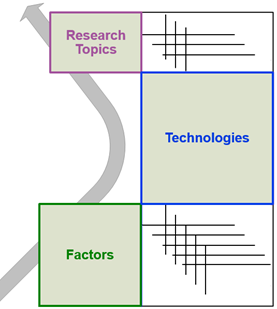
\includegraphics[width=0.49\textwidth]{figures/TradeStudy/figure1.png}
        \caption[Top-level trade study approach used in the HARI analysis]{Top-level trade study approach used in the HARI analysis.}
        \label{figure:tradestudyapproach}
    \end{center}
\end{figure}
To understand the HARI trade space, we reviewed relevant literature across the past ten years and interviewed ten subject matter experts (SMEs) across industry and academia to investigate the current state of HARI technology, challenges facing development, upcoming automation/robotic technologies across a wide range of fields, and opportunities for advancing the state of the art through directed research.
Based on the gathered information, we derived a list of HARI research topics essential to addressing HARI development challenges and advancing the state of the art, as well as a list of specific HARI technologies with application toward HAR tasks common to either long duration deep space exploration (orbital) missions, space surface exploration missions, or both.
An initial set of factors for assessment of technologies was developed.
These factors were characteristics of technologies that effect the potential impact of development on NASA missions, or overall return on research investment.
Factors included HAR task applicability, task (capability) enabling, potential to reduce or introduce risk, and Technology Readiness Level (TRL), among others.

Factors were provided to a group of NASA HARI stakeholders from NASA Ames Research Center and NASA Johnson Spaceflight Center.
They were asked to review eight factors and rank them from most important to least important for consideration of HARI technology investment potential.
NASA stakeholders were informed that these factors would be weighted and used to conduct a trade study designed to help NASA prioritize which technologies and, consequently, which HARI research topics, should be pursued in support of future long duration exploration missions.
After gathering their input, the stakeholder's scores of the factors were averaged and ranked.
The final ranks were used in our trade analysis.

A multi-dimensional trade analysis was performed to objectively assess HARI research topics and specific technologies.
The factors for assessment were traded directly with HARI technologies, while research topics were assessed through direct relationships with those technologies.
Technologies were first assessed against each factor in a series of individual one-dimensional trade analyses (each trading technologies against one factor).
The results of these factor-level trades were normalized and used to score technologies, taking into account the relative factor weights, in the factor-to-technology dimension of the larger analysis (Figure~\ref{figure:tradestudyapproach}).
The research-topic-to-technology dimension was assessed based on relationships between the two.
Research topics and technologies were defined as related if a given technology supports the research topic such that its development would fundamentally drive investigation of that topic.
The scores for each related technology for a given research topic were summed to achieve the total score for that topic.

The top-ranking research topics were: (1) Improving training for HAR systems and tasks, (2) Establishing appropriate trust in automation/robotics systems, and (3) Understanding human intent.
The top-ranking technologies identified from the trade study were: (1) Machine Learning, (2) Autonomous obstacle detection/imaging, (3) Robotic/human information interfaces, and (4) Artificial Intelligence.
These results reflect the surveyed background literature and the information gathered from our SMEs.
These top-ranking research topics were driven by their associated highly scoring technologies, while the top-ranking technologies have seen enormous advancements in research interest and development over the past few years, and all offer a large benefit to the tasks required by NASA on future missions.
The top-ranking technologies all benefited from high marks across all factors.

Based on the trade analysis performed, it is recommended that NASA prioritize research investment in the topics of improving training for HAR systems and tasks, establishing appropriate trust in autonomous/robotic systems, and understanding human intent.
These top-ranked research topics can be traced to trends of broad task applicability, high potential for risk reduction, low potential for risk reduction, and are areas whose study supports the advancement of research in lower-ranked topics as well.
Investigation of these research topics will provide a fundamental foundation for addressing challenges that face implementation of HARI technology solutions in future exploration missions.

\section{Introduction}
Technological advancements in automation and robotics necessitate appropriate integration between these systems and their human operators.
To date, there has not been a systematic evaluation of the HARI design challenges for human spaceflight critical to current and upcoming automation/robotic technologies.
Industries like transportation, air traffic management, and defense are investing significant time and effort to investigate and solve the many design challenges involved in human-automation/robotic integration.
NASA's Human Factors and Behavioral Performance Element needs to understand the critical human-automation/robotic integration design challenges for future space exploration.
A survey of the upcoming research topics and technologies which can be applied to NASA from a range of industries and domains is needed in order to reduce the risks associated with human spaceflight.

Therefore, an assessment of the upcoming technologies and open research challenges critical to effective human and automation/robotic integration (HARI) systems across industries and domains is essential to inform the design and development of safe, efficient future systems.
The objective of the current project is to conduct a systematic assessment of the space-relevant HARI automation/robotic technologies in order to prioritize necessary research required for successful human performance and HAR integration.
This includes identification of aspects that influence the relative importance of technology for spaceflight, or factors, for assessing prioritization of HARI related research and technologies.

\section{Project Background}
The overall objective of this study was to investigate HARI technologies on the horizon with the potential to support critical HAR tasks and use trade analysis to assess these technologies against critical factors for investment in order to determine recommendations for research and development.
The project was designed with two Phases, with Phase 1 focused on gathering background information and identification of specific technologies, and Phase 2 focused on trade analysis.
Tasks were originally proposed for each Phase as shown in Tables~\ref{table:phase1} and~\ref{table:phase2}.
This project largely followed the original two-phase plan, with background research informing the design of a trade study aimed to provide recommendations of technologies/research to pursue.
However, specific tasks were redirected, in coordination with the Human Automation / Robotics Integration (HARI) Discipline Scientist (DS) (NASA Civil Servant at Ames), as we gathered the background information in Phase 1 and learned more about the trade space.

In exploring HARI technologies and risks and challenges facing development, as described in the Phase 1 tasks, through literature review and interviews with Subject Matter Experts (SMEs), it became evident that technology implementations as described in Task 1.3 would vary widely due to dependence on specific mission design, even when constrained to a specific HAR task.
It would not be possible or practical to capture the space of all possible specific technology implementations at such a detailed level.
The primary goal of this project was to explore a trade space of HARI solutions or directions for research, not to trade on mission designs.
Rather than explore a subset of implementations whose applicability to a HAR task would be limited mission to mission, we chose to raise the level of the technology/research trade space and explore broader solutions to HARI challenges as they apply to HAR tasks common to the scope of long duration orbital and planetary surface exploration missions.
For example, exploring the potential of Augmented Reality/Virtual Reality (AR/VR) technology in general as applied to HAR tasks, as opposed to a specific implementation of AR/VR to train for surface operations that assumes a human-robot team makeup (a mission design decision).

In reviewing a draft of the report described in Task 1.5, it became apparent that the HARI solutions identified fell into two categories.
While some were technologies which support or enable HAR tasks, others were research topics related to those technologies whose study will fundamentally drive future HARI capabilities and directly address HARI challenges.
Given the importance of the research topics identified for addressing HARI risk, the trade analysis plan was directed to capture both technologies and research topics (and the relationship between them).
Additionally, with each technology and research topic applicable to a range of HAR tasks as described above, rather than having a separate analysis for each task, HAR task became a critical factor for comparison across the trade space, providing a more complete evaluation between technologies.
Although the process outlined in the Phase 2 tasks was followed, the focus of the trade analysis was shifted to reflect the nature of the trade space.
This shift allowed the study to produce relevant recommendations on closing HARI risk as intended.

\begin{table}[tb]
    \centering
    \includetable{hari-phase1.tex}
    \caption[Tasks initially proposed for Phase 1 of the HARI Trade Analysis]{Tasks initially proposed for Phase 1 of the HARI Trade Analysis.}
    \label{table:phase1}
\end{table}

\begin{table}[tb]
    \centering
    \includetable{hari-phase2.tex}
    \caption[Tasks initially proposed for Phase 2 of the HARI Trade Analysis]{Tasks initially proposed for Phase 2 of the HARI Trade Analysis.}
    \label{table:phase2}
\end{table}

\section{Background Research}
To begin the assessment of space-relevant HARI critical factors, we first completed a comprehensive literature review of the field of human and automation/robotics interaction.
Background literature primarily focused on survey papers from the past ten years, but also included prominent papers from noted authors in the field.
Primary research was also gathered from discussions with subject matter experts in human factors and human-robot interaction related fields.
Findings and lessons learned from this investigation are provided in this report.

\subsection{Literature Review}
We completed a review of human factors and automation/robotics integration survey papers published over the past decade, with an increased focus on the past five years.
Non-survey papers from highly cited and established experts were also added to this review to provide additional insights.
When reading these papers, care was taken to note recurrent topics and technologies that received specific focus, were forecast to generate additional interest in the near future or were otherwise noted as requiring greater study.

As a result of this literature review, major themes of in human and automation/robotic integration technology development and research were identified, see Table~\ref{table:key-papers}.

\begin{table}[tb]
    \centering
    \includetable{hari-key-papers.tex}
    \caption[Table of the key papers reviewed]{Table of the key papers reviewed, and the topics discussed in each.}
    \label{table:key-papers}
\end{table}

Each of these topics is briefly discussed below, referencing their fundamental papers when possible, as well as their forecasts from the previously reviewed articles.

\subsubsection{Machine Learning}
Machine learning (ML) is among the most commonly mentioned topics which authors forecast as being essential to the future of human-robotic interaction~\citep{wang_current_2018}.
Machine learning has enabled significant benefits in a variety of automation/robotics systems but has also given rise to the need for explainable systems and has raised additional questions about trust.
While machine learning techniques may be effective, they are rarely easily explainable, and operators often have difficulty understanding exactly why a system behaves as it does.
Additionally, as these systems have become more sophisticated, they have become able to continuously learn and update their behavior, making it challenging for operators to maintain both system understanding and appropriate levels of trust~\citep{chen_humanagent_2014}.

Machine learning techniques such as hidden Markov models, Gaussian mixture models, and radial basis function neural networks, though usually requiring a supervised training phase, have been shown to be very effective in predicting human intent in the context of physical human-robotic interaction~\citep{losey_review_2018}.
In reviewing which machine learning algorithms are currently being used, Zamora et al. found that neural networks accounted for an overwhelming majority, but that both supervised and unsupervised algorithms were about equally common~\citep{zamora_machine_2017}.
ML is essential to the fields of vision-based hand gesture recognition and non-visual gesture recognition, without which gesture recognition devices would be impossible~\citep{liu_gesture_2018, rautaray_vision_2015, 8701742}.
As computer technology continues to rapidly advance, the ability to detect, track, and classify gestures in real-time has enabled this technology to be implemented in manufacturing and other industrial plants.
Liu et al. specifically call out a need to combine different ML algorithms to improve efficiency, and that deep learning techniques are now enabling non-wearable sensors~\citep{liu_gesture_2018}.
ML has also been used to vary the personality and behavior of adaptive social robots~\citep{ahmad_systematic_2017}.

In her 2017 paper, Endsley noted the research needs for the next thirty years of designing and building fully autonomous systems~\citep{endsley_here_2017}.
Several of these specifically concern machine learning techniques, including validating autonomy software, learning system consistency and transparency.
There are currently no effective techniques for validating autonomy software, as ``traditional methods fail to address the complexities of learning systems.
Exhaustive testing of rules and potential system states will not be possible and understanding boundary conditions will be difficult''~\citep{endsley_here_2017}.
Validating machine learning solutions is currently an active area of research.
There is concern about consistency in learning systems, as different systems will learn using different techniques and provide different levels of feedback about how their automation has changed based off new data.
Endsley notes the lack of transparency in learning systems as a unique challenge, saying ``[t]he actual logic and lessons 'learned' by neural networks and deep learning software are typically opaque not only to the human operator but also to software developers who may not fully understand how the system will behave in all circumstances''~\citep{endsley_here_2017}.
These problems are exemplified by \citeauthor{sheridan_humanrobot_2016}, who notes that ``[i]t is becoming clear that many complex traffic situations are exceedingly difficult for computer vision and artificial intelligence to 'understand' and that many accidents are avoided by social interaction between drivers, such as mutual eye contact, hand signals, and so on.
Understanding the social aspects of driving in traffic, as well as the degree to which cars can be safely automated, demands much further research.''

\subsubsection{Flexible, Adaptive, or Adaptable Automation}
Flexible, adaptive, and adaptable automation are widely praised in the literature for their ability to provide dynamic levels of automation.
The flexibility to provide different sets of automated features during different mission phases, for instance, is an effective requirement for many modern tasks.
One example of this is the autopilot software used in modern transport aircraft, which includes multiple modes of automation for takeoff, cruise, and landing.
~\citeauthor{chen_humanagent_2014} define flexible automation as ``systems that invoke various levels of automation depending on the operator's state, critical events in the environment, or algorithms related to specialized problem sets.''
Chen and Barnes and others have subdivided flexible automation into subtypes, based on the involvement of humans in the decision making process: adaptive automation—where tasks are assigned using conditions established before a mission, adjustable automation—where the human decides when to invoke automation, and mixed-initiative systems—where both the human and the system jointly decide how to allocate tasks~\citep{chen_humanagent_2014, beer_toward_2014}.
These dynamic changes in the role of the human in the human-automation interaction are meant to ``either increase the robot's level of autonomy at the expense of the human's authority, or, conversely, increase the human's control over the shared cooperative activity at the expense of the robot's autonomy''~\citep{losey_review_2018}.
These systems help maintain overall performance while attempting to reduce workload and maintain situational awareness for their human operators~\citep{kaber_situation_2006}.

Among these three automation technology areas, adaptive automation has seen the most research, and many authors have involved it in empirical studies~\citep{vagia_literature_2016}.
The primary difficulty with adaptive automation lies in ``thorny human factors issue of [function] allocation...which has been met with marginal success''~\citep{vagia_literature_2016}.
Optimal assignment of tasks between the operator and the system is difficult as it requires excellent understanding of the performance of the operator and the system's response to the operator.
It also requires the operator to be fully aware of the functional allocation at all times, otherwise mode confusion may occur.

Flexible automation can react to dynamic changes in the environment, and researchers have been able to include real-time sensor data of human physiological states to bring the operator's workload and situational awareness into the loop.
Monitoring the human allows the system to automatically take over tasks when workload is high, and has been used to send control back to the human when the system notes that they have become complacent or as an attempt to increase situational awareness~\citep{lu_human_2016}.
This type of automation is already present in self-driving vehicles on the road today—self-driving vehicles require that drivers have their hands on the wheel even when in self-driving/lane-keeping modes.
While this flexible automation is often effective in common and well understood systems such as driving, there is some concern that flexible automation may prove detrimental in complex and potentially unpredictable systems such as robotic swarms~\citep{kolling_human_2016}.

While adaptive and adaptable automation has been the subject of many experiments over the past few decades, the question of who should be in charge of setting the level of automation remains an open question in need of further study, though mixed-initiative systems may provide the best of both worlds~\citep{chen_humanagent_2014, parasuraman_humans:_2008}.
\citeauthor{chen_humanagent_2014} conclude their review by noting that ``[m]ixed-initiative architectures take advantage of the synergy between the more sophisticated worldview of an experienced human as well as the agent's logical precision and more rapid latencies.''
This architecture is inherently complex and difficult to study, however, as individual differences such as age, expertise, and trust have large effects when interacting with these systems~\citep{schaefer_meta-analysis_2016}.
Further research is recommended into different types of flexible automation, especially when it deals with very complex systems.

\subsubsection{Networked Multi-robot Systems and Swarms}
Human automation/robotics interaction has traditionally focused on a single robotic system, but the miniaturization of computer technology has made swarm or multi-robot systems an increasingly viable option.
The ability for swarms to dynamically reconfigure themselves in response to changing environmental variables and task demands, however, can lead to complex requirements on the human operator.
There remain important questions to be answered in the realm of human systems integration with swarms, especially regarding human supervisory control~\citep{kolling_human_2016}.
There is a specific concern with monitoring human workload and situational awareness as the number of robots increases.
Depending on the number and ability of robots and the type of tasks being performed, it is possible to quickly overburden the swarm operator, especially when operator is required to negotiate swarm-swarm interactions.
\citeauthor{kolling_human_2016}'s \citeyear{kolling_human_2016} review breaks the cognitive complexity of the human-robot system into three complexities: robots performing independent activities, with complexity O(n), which allows more robots to be controlled simply by adding more operators in a linear manner; robots interacting with other robots fully autonomously, with complexity O(1), which allows for a fixed number of robots to control any number of robots; and the case where robot-robot interaction must be controlled by an operator, with complexity O($>$n), as the dependencies between robots results in more demand faster than the number of robots grows.
See Figure~\ref{figure-hari:controlcomplexity} for a graphical illustration of control complexity under each of these conditions.

\begin{figure}[b!]
    \begin{center}
        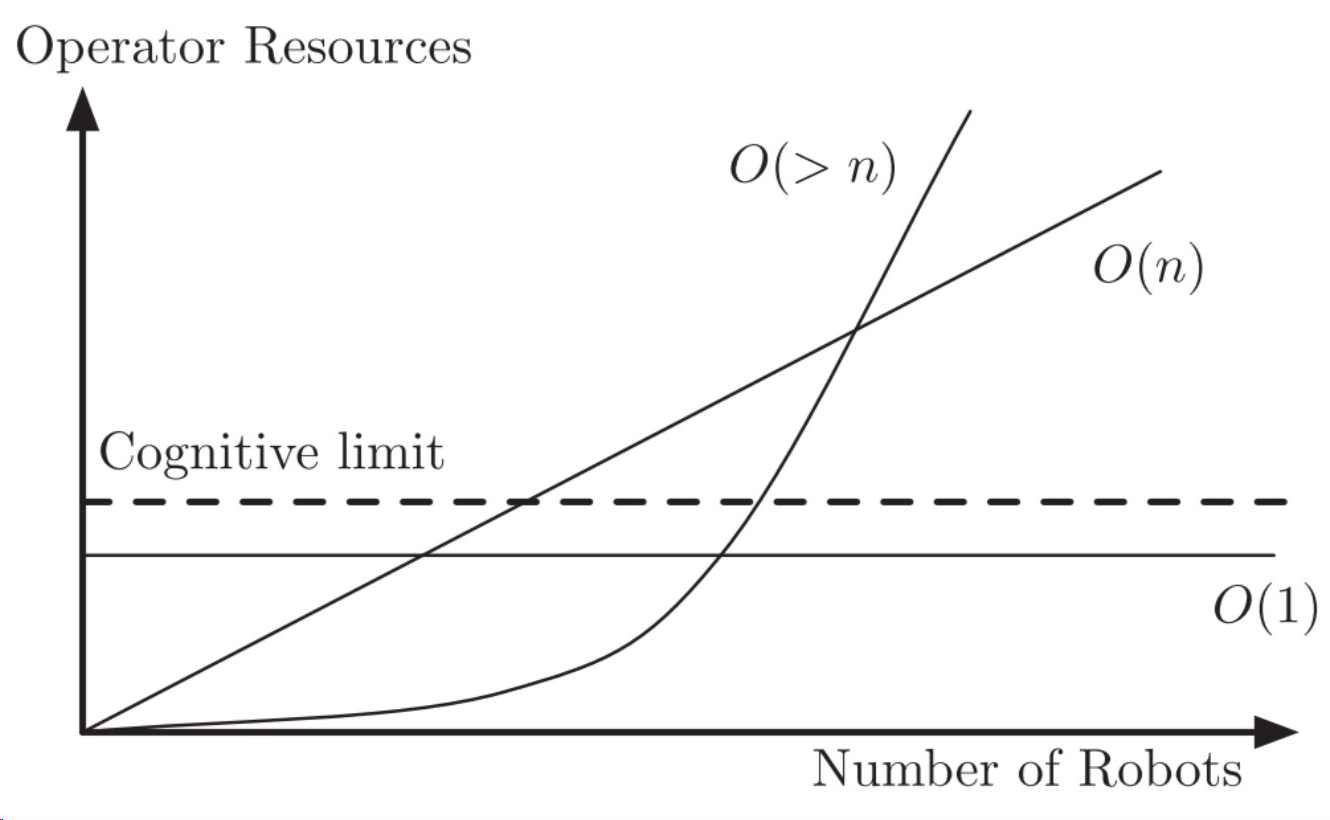
\includegraphics[width=0.8\linewidth]{figures/TradeStudy/figure2.png}
        \caption[Control complexity in a human–multirobot system]{Graphical illustration of the concept of control complexity in a human–multirobot system~\citep{kolling_human_2016}.}
        \label{figure-hari:controlcomplexity}
    \end{center}
\end{figure}

Ongoing research into human-swarm interaction and multi-robot systems has primarily focused on coordinated swarm control, changing swarm topology, and describing the state of the swarm in a more understandable way~\citep{wang_current_2018}.
The development and design of human-swarm interfaces for multi-robot collaboration and, particularly, unmanned aerial vehicle teams is another important set of ongoing research.
The ability for swarms to multitask, and the requirement for the human operator to quickly task switch has been shown to cause detrimental effects on overall system performance~\citep{chen_humanagent_2014}.
High workload phases have been shown to be most sensitive to interruptions from tasks switching, suggesting that task switching should be avoided during these phases unless absolutely necessary~\citep{norman_user_1986}.
Issues relating to multitasking, task switching, and the loss of situational awareness can be mitigated with properly designed human-swarm interfaces.
\citeauthor{chen_humanagent_2014} outlined several of the prominent issues in user interface design and offered solutions in the form of guidelines.
They identified six issues range from ``maintaining operator's ultimate decision authority'' to ``visualization and training techniques enhance human-agent collaboration'', and present guidelines based on the findings of their review.

The concept of robots and automation systems that rely on externally networked support has also been explored by researchers~\citep{kehoe_survey_2015}.
New topics of research using ``the cloud'' or otherwise networked robotics include big data, cloud computing, collective robot learning, and human computation, see Figure~\ref{figure-hari:cloudrobotics}.
Other key technologies which can be enhanced with networked robotic systems include human-robot collaboration technology, autonomous navigation technology under non-structured environments, multi-agent robot systems (swarms), and emotion recognition and interaction mechanism of robot oriented to harmonious human-robot cooperation~\citep{wang_current_2018}.
Issues associated with the rise in cloud technology include the need for techniques to consider time varying latency and quality of service, system security from remote intrusion, privacy concerns, and big data cleaning and filtering techniques.
Currently, cloud computing can be described as a framework with consists of three levels: Infrastructure as a Service (IaaS), where bare operating systems are available; Platform as a Service (PaaS), where more structure is provided, including access to application frameworks, databases, and programming languages; and Software as a Service (SaaS), where software is made available online rather than as a local service~\citep{kehoe_survey_2015}.

\begin{figure}[b!]
    \begin{center}
        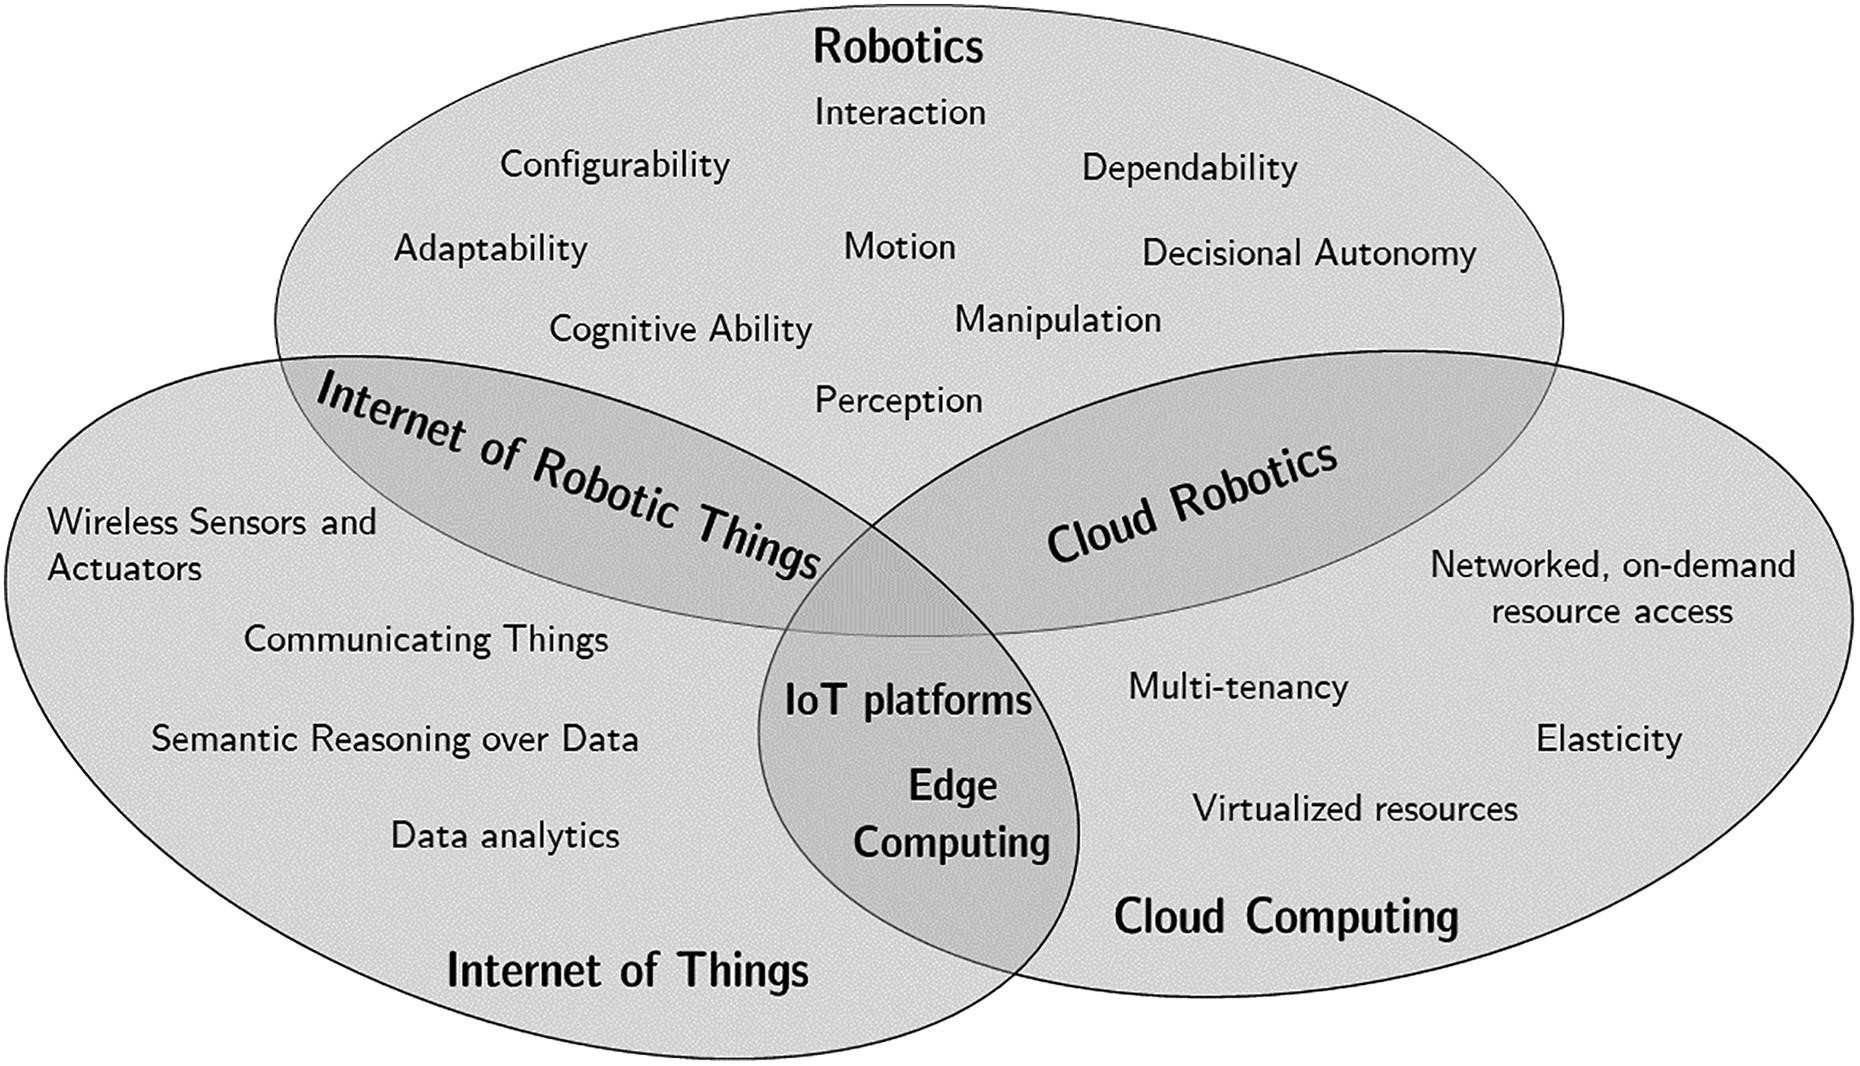
\includegraphics[width=0.8\linewidth]{figures/TradeStudy/figure3.jpg}
        \caption[Cloud Robotics]{Combining Robotics, the Internet of Things, and Cloud computing has resulted in many new possibilities such as Cloud Robotics~\citep{simoens_internet_2018}.}
        \label{figure-hari:cloudrobotics}
    \end{center}
\end{figure}

\subsubsection{Trust}
Human trust has numerous definitions but for our purposes can be considered to be ``the attitude that an agent will help achieve an individual's goals in a situation characterized by uncertainty and vulnerability''~\citep{lee_trust_2004}.
Trust has become an increasing topic of research as robotics increasingly moves out of traditional settings such as manufacturing and into more common-place locations such as the office and the home.
Trust has a large impact on the physical safety of people operating around robots, as improper trust can lead a person to inadvertently place themselves in harm's way.
Considering the ways that trust changes over time has been an important aspect of the research into trust, and \cite{schaefer_meta-analysis_2016} define trust as a three-dimensional expression of a relational property:
\begin{enumerate}
    \item An individual's overall, long-term propensity to trust in general
    \item A transient, momentary trust responsive to immediate ambient conditions
    \item How 1) and 2) evolve over time
\end{enumerate}
Their meta-analysis found strong effects between human-robot interaction and analyzed the factors that determine trust.
A robot or robotic system's ability to garner trust relies on several factors.
See Figure~\ref{figure-hari:trust} for \citeauthor{schaefer_meta-analysis_2016}'s conceptual organization of influencing the development of trust.
Trust is commonly assessed using surveys, many of which have been proposed, which attempt to measure the individual factors which establish trust.
These scales attempt to measure individual elements of trust, asking about the operator's assessment of the automation's competence, predictability, and dependability, among other factors.
Of these measurement techniques, two of the most commonly used scales are the ``Checklist for Trust between People and Automation''~\citep{jian_foundations_2000} and versions of \citeauthor{muir_trust_1996}'s subjective rating scales, though research into real-time techniques is ongoing~\citep{SEPPELT201966}.
Appropriate trust is important when shared control between human-robot teams is essential, as the human is more likely to arbitrate additional tasks to the robot when this trust is established~\citep{losey_review_2018}.

\begin{figure}[b!]
    \begin{center}
        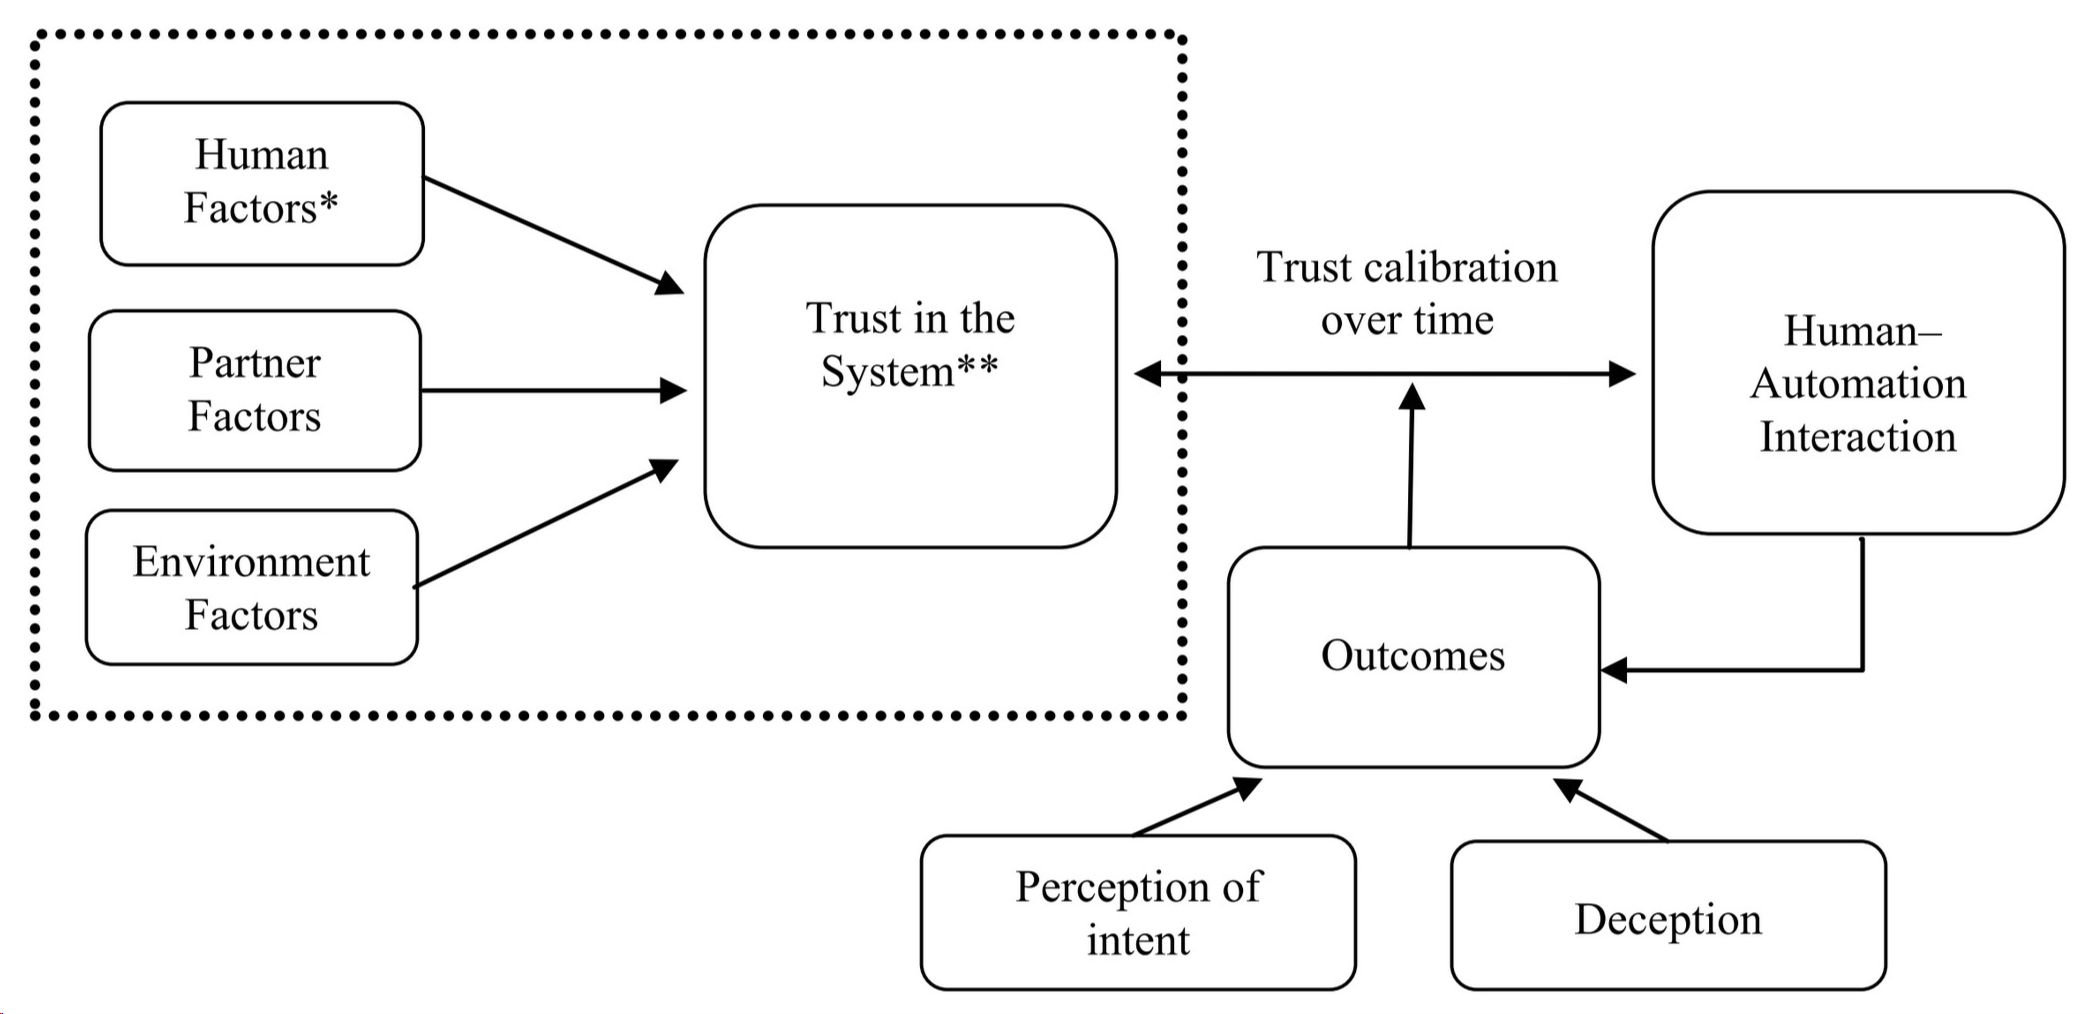
\includegraphics[width=0.8\linewidth]{figures/TradeStudy/figure4.png}
        \caption[A conceptual organization of trust influences highlighting trust development]{A conceptual organization of trust influences highlighting trust development~\citep{schaefer_meta-analysis_2016}.}
        \label{figure-hari:trust}
    \end{center}
\end{figure}

\citeauthor{ososky_building_2013} made several propositions regarding human trust of robotics, among the most important being that:
\begin{itemize}
    \item Humans are easily influenced by superficial characteristics of robots
    \item Human subjective assessment of trust in robots ultimately determines the use of robotic systems
\end{itemize}
They noted that robot characteristics had the strongest influence on trust in human-robot teams, which included factors such as reliability, transparency, and anthropomorphic qualities.
One example of this is \citeauthor{de_visser_almost_2016}'s \citeyear{de_visser_almost_2016} study, which found that anthropomorphic automation associated greater trust resilience.
\citeauthor{de_visser_almost_2016} concluded their study by suggesting that designers incorporate these features into future robots as a deliberate design choice to garner greater trust.
Even very simple additions such as high levels of mutual gaze have been shown to increase trust, while gaze aversions stoke feelings of distrust between human-robotic teams~\citep{admoni_social_2017}.

While anthropomorphism can lead to greater trust, some authors note caution when incorporating these features.
\citeauthor{culley_note_2013} warn that individual differences can lead some individuals to place too great a trust in anthropomorphic robots.
Individuals are even more likely to trust anthropomorphic robots if they perceive similarities to the robot and themselves regarding age, gender, and even similarity of movement~\citep{pak_multi-level_2014, verberne_trusting_2013}.
Ososky further warns that trust in a robot's reliability alone is insufficient for better teamwork, and that over-trust combined with an inaccurate or incomplete mental model can lead to worse overall performance.
This is especially important when considering changing levels of automation in the field of human-automation interaction, for example, as an operator may not fully understand what they are currently responsible for, if the robotic system is in control.
This has led to numerous incidents leading to serious injury and death.
Trust in human-robot teaming is slightly different than trust in automation, however, as robots are often seen as collaborating teammates rather than just an automated tool~\citep{ososky_building_2013}.

\subsection{Interviews with Subject Matter Experts}
In order to provide a current assessment of the critical challenges associated with effective HARI systems across industries and domains, we also interviewed subject matter experts (SMEs).
SMEs were chosen to represent a cross section of HARI related disciplines such as aerospace, industrial robotics, military applications, medical, and autonomous vehicles.
SMEs were intentionally selected from different backgrounds, including military research, academia, and industry (robotics, medical, aerospace), in order to provide broad perspectives on the risks and challenges facing HARI technology development, as well as HARI technology and research.
We conducted ten phone interviews with SMEs who integrate humans, automation, and robotics in their work.
These interviews generally took between twenty and forty minutes.
We asked each expert the following questions:
\begin{enumerate}
    \item What technologies do you think are on the horizon in your field in the integration of humans, automation, and robotics?
    \item How would you prioritize what technologies are in development involving the integration of humans, automation, and robotics?
          \begin{enumerate}
              \item What technologies would be the most responsive to increased research support?
              \item For these technologies, what are the current TRLs? How much effort do you think it will take to raise the TRL over time?
          \end{enumerate}
    \item What are you most concerned about for the integration of humans, automation, and robotics? What technologies do you think could mitigate these risks?
          \begin{enumerate}
              \item What risks do you see arising from inclusion of these technologies (what new risks do you anticipate)?
              \item What risks currently have no technology solutions?
          \end{enumerate}
    \item How will these technologies fill the gaps in our current abilities?
          \begin{enumerate}
              \item Where do you see additional automation as a plausible way to fill those gaps?
              \item What other technology gaps should we be concerned about?
          \end{enumerate}
    \item Based on this discussion, is there anything else we should know?
\end{enumerate}

Based on the information gathered from literature and discussion with subject matter experts, the following specific HARI-related technologies and research topics emerged as areas for future research and development for the advancement of human automation and robotic interaction relevant to human spaceflight.

\subsection{Specific Technologies}
\subsubsection{Non-invasive behavioral and physiological sensing}
Non-invasive behavioral and physiological sensing includes a range of techniques.
Some physiological sensing techniques include common place, if controversial, methods such as a polygraph, to electromyography (EMG), electroencephalogram (EEG), and electrocardiogram (EKG) sensing.
Behavioral analysis techniques can include techniques that rely extensively on video analysis, such as gait analysis, and more integrated technology covering additional modalities.
This technology can be used to infer team member states.
The use of artificial intelligence to combine these perceptions is relatively developed.
This technology has an estimated TRL range of 3-5.

\subsubsection{Implantable Biometrics}
Compared to many of the other specific technologies we identified, implantable biometrics is a relatively young field which focuses on implantable biosensors for precision and personalized medicine.
These sensors can provide continuous data on specific, targeted metrics which can allow for the immediate detection of problems or need for intervention.
Implantable biometrics is especially important in the ``diagnosis, monitoring, management and treatment of a variety of disease conditions'' and can be used to detect changes in a person's health~\citep{fitts_human_1951}.
Further advances in miniaturization and nanotechnology are likely needed for this technology to advance further.
This technology has an estimated TRL less than 3.

\subsubsection{Autonomous obstacle detection/imaging}
Autonomous obstacle detection/imaging is a combination of technologies designed to identify obstacles around a robot or other autonomous agent.
Detection and imaging can make use of visual spectrum or other light sources, acoustic or magnetic sensors, or laser-based technologies such as LIDAR.
Multiple techniques also take advantage of combining these technologies into multispectral sensors.
These technologies are important for autonomous docking and landing of spacecraft but have also seen an enormous increase in interest from the self-driving car industry.
One important side effect of increased demand of this technology in self-driving cars in the past few years is that the hardware has both rapidly miniaturized and dropped in price.
Note that this technology is only concerned with detection, while resulting actions and path planning is captured elsewhere (autonomous path planning).
This technology has an estimated TRL of 6 or greater.

\subsubsection{Autonomous path planning}
In contrast to autonomous obstacle detection, autonomous path planning describes the resultant planning and action that is taken after an obstacle is sensed or an objective is determined.
This technology benefits greatly from a good understanding of the robot or autonomous agent's dynamics, the environment it acts in, other agents in the environment, and the objective's location.
With regards to spaceflight, autonomous path planning is relevant when considering orbital proximity operations (including rendezvous and docking), surface landings, and rover movements.
This technology has also seen great benefits from the self-driving car industry, especially regarding planning around other moving agents whose intent is often poorly understood.
This technology has an estimated TRL of 6 or greater.

\subsubsection{Speech recognition}
Speech recognition is a set of technologies that enable the translation of spoken words to text by computer software.
Speech recognition has been actively developed since the 1970s and has a generally high rate of success.
Despite this relatively long period of development, recent advancements in speech recognition have been made by integrating machine learning techniques.
Transforming spoken word to text allows autonomous systems and robots to accept commands or infer human intent and is a common alternative to physical computer interfaces~\citep{tsarouchi_humanrobot_2016}.
It also allows for the detection of speech patterns and inflection classification to capture intent, trust, fatigue, or emotional states.
Depending on the system and application, speech recognition systems have higher TRL in the range of 6 or greater.

\subsubsection{Intuitive control interfaces}
Intuitive control interfaces consider ways of intuitively mapping human gestures to a resultant robotic action, and often takes human physiology, kinematics, and other elements of physical movement into consideration.
This technology includes interfaces types such as joysticks, keyboards, touchscreens, and gesture recognition, among others.
This technology has an estimated TRL of 6 or greater.

\subsubsection{Robotic/human information interfaces}
Information displays must determine what information to transmit for any given task, which may be customized based on user preference, task or environment concerns, past experiences, or the presence of anomalies.
These may include multimodal (visual, audio, and/or haptic) displays which display task relevant information to an operator.
They may display 2D or higher-dimensional information and may be body-worn or mounted in the environment.
These displays have elements designed by both human-computer interaction experts and machine learning algorithms.
Ideally, such displays would be ubiquitous, capable of quickly and easily transferring information between stations, and able to appear on traditional monitors, tablets, smartphones, or augmented reality interfaces.
While some elements are well-defined and arguably in use today, others remain in early stages of development.
Based on feedback, these systems have a current overall TRL estimated at 3-5.

\subsubsection{Augmented Reality and Virtual Reality}
Augmented and virtual reality are a pair of technologies which provide a partial or fully virtual environment to a user, often in the form of a head mounted display.
Augmented reality has also been developed to work with modern phones and tablets, and can provide additional, digital context to an otherwise physical object or environment.
Virtual reality is increasingly used as a training tool, while augmented reality has begun to be used as a tool for both training and operations.
This technology has an estimated TRL of 3-5.

\subsubsection{Robotic agents}
This technology encompasses a large variety of robots, which include rovers, satellite or UAV swarms, robotic arms, and vehicles, among others.
The relative TRL varies between relatively low, in the case of robotic swarms, to very high, in the case of rovers and robotic arms.
These sets of technologies enable humans to complete tasks that they could not otherwise accomplish, either because they take place in an extreme, dangerous or difficult to reach environment (as is the case with Martian rovers), they require abilities humans do not (moving payloads required by robotic arms such as Canadarm2) or because they would take too long (such as the mapping or scouting of a region by a swarm of UAVs or satellites).
On average, TRL may be estimated within the range of 3-5.

\subsubsection{Assistive Robotics}
In contrast to robotic agents, which largely replace the human or do not require a human to be present, assistive robotics describe robots that directly interface with humans to assist them in accomplishing a task.
These robots include small assistive satellites such as Astrobee, a modern version of the Apollo Lunar Roving Vehicle with more advanced guidance capabilities, exoskeletons, or personal assistants.
These robots enhance the already existing abilities of humans by enabling them to complete tasks that they otherwise could not, or by increasing performance in challenging tasks.
This technology has an estimated TRL of 3-5.

\subsubsection{Artificial Intelligence}
Artificial intelligence is intelligence demonstrated by machines, in contrast to human intelligence.
Some of the major goals of AI include knowledge reasoning, planning, natural language processing, computer vision, robotics, and machine learning.
In space HARI, AI could primarily be leveraged in managing complex systems (i.e. diagnostics, prognostics, and maintenance of spacecraft) and in acting as assistants for crew completing science and activity tasks.
By correctly interpreting human intent, AI can also control robots for payload and physical crew assistance.
This technology has an estimated TRL of 3-5.

\subsubsection{Machine Learning}
Machine learning describes a collection of algorithms which perform a specific task without using explicit instructions, instead relying on learned models.
Common types of machine learning include supervised learning, in which a human trains the model, unsupervised learning, where the system learns on its own, and reinforcement learning, where the software takes actions in an environment to optimize a cost function.
Machine learning has improved the performance of many varied technologies and is the foundation on which artificial intelligence is being developed upon.
This technology has an estimated TRL of 6 or greater.

\subsubsection{Flexible, Adaptive, or Adaptable Automation}
As noted earlier in the report, flexible, adaptive, and adaptable automation are widely praised in the literature for their ability to provide dynamic levels of automation.
The flexibility to provide different sets of automated features during different mission phases, for instance, is an effective requirement for many modern tasks.
\citeauthor{chen_humanagent_2014} define flexible automation as ``systems that invoke various levels of automation depending on the operator's state, critical events in the environment, or algorithms related to specialized problem sets.''
This technology has an estimated TRL of 6 or greater.

\subsection{Research Topics}
\subsubsection{Understanding human intent}
The topic of understanding human intent is wide, and includes subtopics such as the robotic interpretation of human intent, understanding human intent unobtrusively, and improving human to robot communication.
The interpretation of human intent by a computer or robot can be done in a variety of ways, including speech, gestures, and other forms of nonverbal communication.
These techniques are at varied levels of development, from basic proof of concept to use in operations.
Each technique can be broken down into several levels—gestures, for example, have four levels: sensor technologies, identification, tracking and classification~\citep{liu_gesture_2018}.
This is area is also closely tied to interpreting behavioral and human monitoring data and encompasses human/behavioral model research such as the prediction of intent from eye movements~\citep{Singh:2018:CPG:3237383.3237457, ruhland_review_2015}.

\subsubsection{Autonomous/robotic system communication to humans}
In contrast to the previous topic (understanding human intent) the research topic of autonomous/robotic system communication to humans addresses how these complex systems can best relay information back to a human operator.
This topic includes both research of communication techniques and mitigation of miscommunications from the system to the human.
This topic deals with discovering effective methods of providing information to a human user in an intuitive way, such that communication feels natural to a human operator.
Human-robot communication is largely focused on developing multisensory methods to successfully communicate a robot's intent to humans.
Human-autonomous system communications additionally deals with methods to successfully enable explainable and transparent autonomous system operation.

\subsubsection{Ensuring human safety (physical)}
This topic captures research which investigates how to enable safe human and robot operation in a shared environment in order to reduce risk.
It specifically investigates methods to successfully prevent harm to humans in close physical proximity with robots and develops guidelines and recommendations as to how physical interaction between robots and astronauts can safely occur.
This research topic benefits from the lessons learned in manufacturing settings, where humans and robots must often work nearby or directly with each other, as well as that work done by autonomous car companies in avoiding pedestrians.

\subsubsection{Continuous human performance monitoring}
The topic of continuous human performance monitoring seeks to understand human-system performance and measure human performance unobtrusively.
This research topic seeks to understand which human-system performance measures and limits are required for spaceflight and seeks to validate novel methods and technologies for measuring a variety of aspects of human performance such as task performance, workload, and situational awareness.
Research in this area also focuses on understanding the human performance effects resulting from adaptive automation and attempts to identify what are the performance differences between adaptable (human sets level of automation) versus adaptive (automation sets level of automation).

\subsubsection{HAR team performance optimization and function allocation}
Human autonomous/robotics team performance optimization and function allocation investigates different ways of understanding human-robot teamwork and human-autonomous system robustness, decides whether a particular function will be accomplished by a person, technology (hardware or software) or some mix of person and technology~\citep{fitts_human_1951}, and how to optimize that balance~\citep{yanco_analysis_2015}.
This research focuses on what social and teamwork elements enable successful human-robot collaboration, especially when it requires direct interaction between robots and astronauts.
With relation to robustness, this area also captures research on how to measure robustness when humans are using system in off-nominal conditions and identifying when these systems are off nominal.

\subsubsection{Enabling command/control of complex robotic systems}
This topic focuses on enabling command/control of complex robotic systems and enabling critical decision making.
This includes research on methods to successfully allow humans to command and control multiple, mixed robotic agents with varying levels of autonomy and flexible function allocation.
It also looks at new methods to enable humans to make time-critical decisions using autonomous systems across a variety of system dynamics and is required to evaluate methods for different autonomous systems with different functions (e.g., ECLSS vs. Power vs. Navigation).

\subsubsection{Improving situation awareness in HAR systems}
One of the most accepted definitions of situation awareness states that ``[s]ituation awareness is the perception of the elements in the environment within a volume of time and space, the comprehension of their meaning, and the projection of their status in the near future''~\citep{endsley2017toward}.
This research topic focuses on techniques to both maintain and improve operator situation awareness when interacting with automation/robotics systems.
Recent work by \citeauthor{endsley_here_2017} has further expanded early models of situation awareness, discussing the emerging problem of loss of operator situational awareness and out-of-the-loop performance problems associated with increasing system autonomy, reliability, and robustness.
This new model for human-autonomy system oversight (HASO), incorporates situation awareness, trust, workload and automation interfaces among the key system design features influencing human cognitive processes involved in successful interaction with automated systems.

\subsubsection{Improving training for HAR systems and tasks}
The topic of improving training for HAR systems and tasks investigates what new methods are required or most effective to train humans to use complex, advanced autonomous and robotic systems.
Research in this area explores different techniques and technologies to improve human performance and reduce workload, and often makes extensive use of mockups, simulations, hands-on walkthroughs, and human-in-the-loop studies.
Many techniques have been explored to improve training, including many kinds of feedback, manual control adaptation, and the use of virtual and augmented reality.

\subsubsection{Establishing appropriate trust in automation/robotics systems}
This research topic focuses on techniques to establish appropriate trust in automation/robotics systems and mitigating changes in trust between humans and these systems.
It explores how trust changes with factors such as communication, reliability, workload, social acceptability, privacy, and transparency.
As noted earlier, it can be challenging for operators to establish appropriate trust as these automation/robotics systems become more sophisticated~\citep{chen_humanagent_2014}.
This research has also focused on shared control between human-robot teams and how tasks are arbitrated to the robot when trust is established~\citep{losey_review_2018}.
Trust research investigates when there is a difference between expected and executed actions, and requirements on systems depending on whether knowledge is collected and maintained by software or by human operator.

\section{Trade Analysis}
In addition to specific technologies and research topics, the information gathered from the literature review and the discussions with subject matter experts was used to identify factors relevant to the assessment of technology or research for future investment.
With all of this information gathered, the factors were refined and used in a multi-dimensional trade study to assess the technologies and research topics as priorities for HARI investment.

\subsection{Factor Assessment with NASA Stakeholders}
In addition to interviewing the human, automation, and robotics integration SMEs, we also surveyed six NASA HARI stakeholders for their input on the trade study.
As NASA stakeholders involved in human, automation, and robotic interaction, we asked them to review eight factors and rank them from most important to least important in consideration of HARI technology for investment.
We also had them rank additional ``secondary criteria'' for the factors related to risk.

Factors are characteristics of a technology that our team, in collaboration the NASA HARI DS, has identified and selected because they are relevant to assessing HARI.
These factors were generated from our review of the background literature and conversations with the SMEs.
NASA stakeholders were informed that these factors would be weighted and used to conduct a trade study designed to help NASA in prioritizing which technologies and, consequently, which HARI research areas, should be further invested in to help with future long duration exploration missions.
After our NASA stakeholders provided their input, we averaged and ranked their assessment of the factors.
The ranked factors appear in Table~\ref{table:factor-ranking}.

\begin{table}[tb]
    \centering
    \includetable{hari-factor-ranking.tex}
    \caption[The ranking of seven factors resulting from feedback from our NASA stakeholders]{The ranking of seven factors resulting from feedback from our NASA stakeholders.}
    \label{table:factor-ranking}
\end{table}

\subsubsection{Task applicability}
Which tasks does the technology have an impact on? This factor characterizes how much impact the technology may have on the various HARI tasks identified for future exploration missions~\citep{marquez2017future}.
We determined if each technology applies to each task in order to measure the technology's applicability to space HARI.
These tasks, common to long duration orbital missions, deep space surface exploration missions, or both, are shown in Table~\ref{table:har-tasks}.

\begin{table}[tb]
    \centering
    \includetable{hari-har-tasks.tex}
    \caption[HAR tasks for spaceflight]{HAR tasks for spaceflight.}
    \label{table:har-tasks}
\end{table}

\subsubsection{Task enabling}
Does the technology enable a new capability? This factor describes how much the technology enables one or more of the various HARI tasks identified for future exploration missions.
HARI tasks are assumed to be critical and must be completed.
We subjectively rated this by classifying the technology as: No effect relative to current technology (score of 0), Improves performance of current capability (score of 1), or Adds new capability (score of 2).

\subsubsection{Potential for reducing risk}
What is the benefit from risk reduction? This factor describes how risk might be reduced by the inclusion of the technology.
Each type of risk was subjectively rated.
Types of risks (secondary criteria) are listed below:
\begin{itemize}
    \item Improved safety: increase astronauts' safety.
    \item Reduced likelihood of system failure: increase overall robustness of system by predicting or preventing failures.
    \item Improved performance: astronauts can work more effectively and efficiently, including reducing physical and cognitive workload.
\end{itemize}

\subsubsection{Potential for introducing risk}
What is the cost from introduced risk? This factor describes how risk might be introduced by the inclusion of the technology.
Each type of risk was subjectively rated.
Types of risks are paired with the types of risk reduction.
Note that, unlike all the other factors, a higher potential for introducing risk has a negative impact on the technologies overall score.

\subsubsection{External investment (outside NASA)}
What is the current research activity going on outside of NASA? This factor characterizes how much research and investment has recently and is currently going into the development of the technology by entities outside of NASA.
This is just research on the technology, not HARI research investments.
We measured this using the publication rate associated with each technology.
The name of each technology was searched for on 6/24/2019 on Web of Science using the following search, where technology is substituted for each:
ALL FIELDS: (technology)
Timespan: 2013-2018.
Indexes: SCI-EXPANDED, SSCI, A\&HCI, CPCI-S, CPCI-SSH, BKCI-S, BKCI-SSH, ESCI, CCR-EXPANDED, IC.
Similarly, the technologies were also searched for in Google Scholar on the same date and with the same time span.
The sums from both searches were used to determine scores for this factor (see Trade Study Approach~\ref{ss:tsapproach}).

\subsubsection{Technology Readiness Level (TRL)}
What is the current TRL? This factor characterizes the maturity level of the technology.
We estimated the technology's current TRL using information gathered from the literature and provided by our SMEs.
TRL was split into three categories: Below TRL 3, TRL 3-5, and TRL 6 or greater.

\subsubsection{Research interest (within NASA)}
What is the current research interest within NASA? This factor describes if the technology has any potential for infusion into NASA missions as determined by the NASA Technology roadmaps/NASA Strategic Technology Investment Plan.
We qualify this by checking if the technology is present on the NASA technology roadmap.

\subsection{Trade Study Approach} \label{ss:tsapproach}
A multi-dimensional trade analysis was performed to objectively score HARI research topics and specific technologies in a recommended order of priority for NASA investment.
The approach used was similar to a Relationship Matrix Decomposition Scheme (RMDS)~\citep{boppe_training}, see Figure~\ref{figure-hari:tradestudy}.
The factors for assessment described above pertain directly to HARI technologies, while research topics are assessed through direct relationships with those technologies, see Figure~\ref{figure-hari:tradestudyA}.
This parallels the RMDS approach of tracing assessment of system configurations and technology options based on objectives/goals through functional options, see Figure~\ref{figure-hari:tradestudyB}.
For the complete trade table used in this study, see Appendix~\ref{appendix:trade-tables}.

\begin{figure}[tb!]
    \begin{center}
        \begin{subfigure}{0.49\textwidth}
            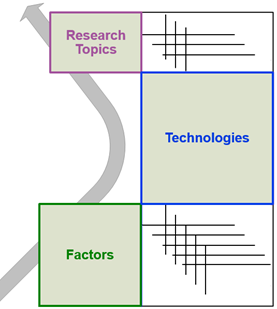
\includegraphics[width=\linewidth]{figures/TradeStudy/figure5a.png}
            \caption[Top-level trade study approach used in the HARI analysis]{Top-level trade study approach used in the HARI analysis.}
            \label{figure-hari:tradestudyA}
        \end{subfigure}\hfill
        \begin{subfigure}{0.49\textwidth}
            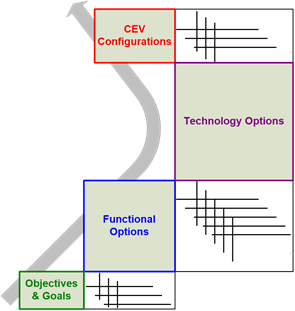
\includegraphics[width=\linewidth]{figures/TradeStudy/figure5b.png}
            \caption[Structure of the RMDS trade study approach]{Structure of the RMDS trade study approach.}
            \label{figure-hari:tradestudyB}
        \end{subfigure}
        \caption[Trade study approaches]{Trade study approaches.}
        \label{figure-hari:tradestudy}
    \end{center}
\end{figure}

Research topics and technologies were defined as related if a given technology supports the research topic such that its development would fundamentally drive investigation of that topic.
Each technology was given a score resulting from the technology-factors dimension of the trade.
The scores for each related technology for a given research topic were summed to achieve the total score for that topic.

The technology total scores represent a roll-up of individual weighted factor scores for each specific technology.
At a factor level, normalized scores for each technology were determined in a series of one-dimensional factor-technology trade studies.
These individual factor-level trades used to compile the factor-technology dimension are found in Appendix~\ref{appendix:trade-tables}.
The factor scores were multiplied by the factor weights as defined in the NASA Stakeholders section of this report and summed for each technology.

\subsubsection{Factor-Level Trades}
The factor-level trades for Risk Reduced, Risk Introduced, and TRL each assessed the specific technologies against three weighted options.
Risk Reduced, for example assigned an individual score of 0 or 1 to each technology if it potentially reduced risk to crew, risk to mission/vehicle, or risk of loss of performance.
Each potentially reduced risk was weighted (1 to 3) based on relative ranking as found by the NASA stakeholders.
The total weighted scores for each technology (sum of weights x scores) were normalized by the highest possible score for a single technology to find the factor scores on a scale between 0 and 1 (see Equation~\ref{eq:weighted-score}, below).

\begin{align}
    \mbox{Normalized Score} =  \frac{{\Sigma}(\mbox{Weighted Scores for a Technology})}{{\Sigma}(\mbox{Weights}) \times \max(\mbox{Individual Score})}
    \label{eq:weighted-score}
\end{align}

For Risk Introduced, normalized scores were multiplied by -1, as introduced risk were tallied as a negative contribution to overall technology assessment.
The TRL trade was performed identically to Reduced Risk, with the exception that technologies could only be assigned to a single average TRL range.
Assessment for Research Interest (within NASA) was simplified compared to other factor-level trades as scoring had a single binary level (trade table included in Appendix~\ref{appendix:trade-tables}).

In the Task Applicability and Task Enabling factor-level trades, scores were assigned between technology and task, with equal weighting across tasks (all assigned a weight of 1).
Technologies were assessed for Task Applicability with a score of 0 or 1, while for Task Enabling technologies were assigned a score for each task of 0, 1, or 2 as described in the NASA Stakeholders section.

In assessment of External Investment in NASA, as described previously, two search engines were used to find estimates on the number of recent publications pertaining to each technology.
Searches with each service are known to poll databases of drastically different size.
The relative database size used by both search engines was accounted for by applying a weight determined by the largest publication total found for each service.
In this way, the relative publication totals for each service could be normalized independently prior to summing the results of the two searches.

\section{Results}

\subsection{Research Topics}
The final scores for research topics have been ranked, such that a high score represents a recommended higher priority for research investment by NASA (see Table~\ref{table:topic-prioritization}).
The top-ranking research topics are:
\begin{enumerate}
    \item Improving training for HAR systems and tasks
    \item Establishing appropriate trust in automation/robotics systems
    \item Understanding human intent
\end{enumerate}

\begin{table}[tb]
    \centering
    \includetable{hari-topic-prioritization.tex}
    \caption[Research topic prioritization]{The resulting prioritization of research topics from linking research topics to the upcoming technologies.}
    \label{table:topic-prioritization}
\end{table}

Note that all these topics were identified as areas applicable to HARI concerns, regardless of the score.
A high score here is highly dependent on the impact of the surveyed technologies on the research topic and suggests which research topics should be able to make relatively quick progress given the technology that is being developed now and in the next 5-10 years.
A low score reflects research topics that either have relatively few technology solutions on the horizon, had relatively low factor scores for the technologies that are related to the topic, or both.

These top-ranking research topics were driven by their associated highly scoring technologies.
Improving training for HAR systems and tasks touches on a variety of upcoming technologies ranging from machine learning to robotic/human information interfaces.
These technologies ranked highly in their task applicability and potential for reducing risk and had relatively little potential for introducing new risks when compared to other technologies.
By leveraging these upcoming technologies, researchers have ample opportunities to investigate novel techniques for improving training for these systems.
These upcoming techniques will prove invaluable as HAR systems and tasks continue to increase in complexity, especially if, for example, they can provide crew with just-in-time training for critical tasks when they are far from the support provided by mission control.
The topic of training came up many times in our conversations with subject matter experts, who often noted case examples of major failures in their explanations for why this training was needed.
Similarly, many subject matter experts also mentioned the need for establishing appropriate trust in automation/robotics systems during our interviews, a topic which came up repeatedly in our review of the literature.
Over-trust and under-trust in these complex systems were both noted as being dangerous and can result from inadequate training.
Research in trust has often focused on its role in flexible, adaptive, and adaptable automation, where operators can be unclear which mode the system is in.
By taking advantage of upcoming technologies in intuitive physical control and robotic/human information interfaces, researchers can help to bring humans into the loop on what is happening within these complex systems.

In contrast to the top-ranking research topics, continuous human performance monitoring and improving situation awareness in HAR systems were among the lowest ranked topics.
While both are important when considering future long duration exploration missions, neither were directly associated with many upcoming technologies.
Despite being associated with the top-ranking technology, machine learning, continuous human performance monitoring ranked lowest.
This is primarily because it was also associated with the two lowest ranking technologies, non-invasive behavioral and physiological sensing and implantable biometrics.
Despite these technologies' clear relation to performance monitoring, they were among the lowest ranking when considering the task applicability and task enabling factors, which were considered the most important by our NASA stakeholders.
Improving situation awareness in HAR systems lower score came as a surprise as situation awareness presents a challenge across all HAR applications.
Although it also benefited from being linked to a top-ranking technology—robotic/human information interfaces—but the topic otherwise suffered from few direct technology solutions.

\subsection{Technologies}
The resulting ranks of the technologies from the weighted factors are shown in Table~\ref{table:technology-prioritization}.
The top-ranking technologies identified from the trade study are:
\begin{enumerate}
    \item Machine Learning
    \item Autonomous obstacle detection/imaging
    \item Robotic/human information interfaces
    \item Artificial Intelligence
\end{enumerate}

\begin{table}[tb]
    \centering
    \includetable{hari-technology-prioritization.tex}
    \caption[Technology prioritization]{The resulting prioritization of technologies using the trade study.}
    \label{table:technology-prioritization}
\end{table}

These top-ranking technologies have seen enormous advancements in research interest and development over the past few years, and all offer a large benefit to the tasks required by NASA on future LDEMs.
In contrast to the top-ranking technologies, low ranking technologies show a trend of reflecting a combination of low research interest, task relevance, or TRL.

The top-ranking technologies all benefited from high marks across all our factors.
Machine learning, our top-ranking technology, particularly stands out due to scoring highest in the External Investment (outside of NASA) factor, where it significantly outperformed the other technologies.
As we noted in the literature review, machine learning came has been repeatedly forecast as being essential to the future of human-robotic interaction~\citep{wang_current_2018}.
It also came up extensively in our conversations with our subject matter experts, though several of these also stressed caution in assuming machine learning could solve any problem without issue.
Artificial Intelligence was also mentioned by most of the SMEs but ranked lower due to its dramatically higher potential for introducing risk.

Autonomous obstacle detection/imaging was our second highest scoring factor but had little impact on our research topic recommendations.
Despite being a well-established technology, the only topic is was ultimately related to was ensuring human safety (physical).
Like our other high scoring technologies, however, it scored well due to its high task applicability, task enabling potential for reducing risk factors.
This suggests that, while the technology should continue to be developed and refined, there is minimal applicability toward ongoing research that addresses outstanding HARI risks and challenges.
Improvements resulting from refinement in the commercial sector, especially regarding autonomous cars, should enable faster and safer algorithms in the future.

Several technologies were highly clustered in the middle of our rankings: autonomous path planning, augmented reality/virtual reality, robotic agents, and flexible/adaptive/adaptable automation also scored within a few tenths of a point from each other.
These technologies all had relatively high potential for introducing risk but were otherwise highly applicable to the tasks related to space HARI.
As noted previously, the two lowest ranking technologies, non-invasive behavioral and physiological sensing and implantable biometrics were among the lowest ranking when considering the task applicability and task enabling factors, which were considered the most important by our NASA stakeholders.
These technologies were also those which did not score in the Research Interest (within NASA) factor, as they were not present in the NASA Technology roadmaps or NASA Strategic Technology Investment Plan.
The third lowest ranking technology, speech recognition, despite being a widespread, high TRL technology, scored poorly because it was the lowest scoring in both the task applicability and task enabling factors.

\section{Contribution (Relation to NASA HARI Gaps)}
NASA has identified four gaps in HARI knowledge, as part of the larger HFBP characterization of human factors risks and associated knowledge gaps~\citep{hari_risk}.
These gaps need to be closed in order to mitigate HARI related risk as it pertains to spaceflight.
The NASA HARI Gaps are:
\begin{itemize}
    \item[\textbf{HARI-01}] We need to evaluate, develop, and validate methods and guidelines for identifying human-automation/robot task information needs, function allocation, and team composition for future long duration, long distance space missions.
    \item[\textbf{HARI-02}] We need to develop design guidelines for effective human-automation-robotic systems in operational environments that may include distributed, non-collocated adaptive mixed-agent teams with variable transmission latencies.
    \item[\textbf{HARI-03}] We do not know how to quantify overall human-automation-robotic system performance to inform and evaluate system designs to ensure safe and efficient space mission operations.
    \item[\textbf{HARI-04}] We need to identify and scope the critical human-automation/robotic mission activities and tasks that are required for future long duration, long distance space missions.
\end{itemize}

This study extends prior investigation of HARI tasks, specifically to address gap HARI-04 directly.
This investigation and trade study identify prioritized lists of specific technologies whose advancement support the activities and tasks required for future space exploration missions, as well as research topics where investment will support both HARI task capabilities and closing of the other three HARI knowledge gaps.
All the research topics identified in this report can assist with closing HARI-02, and most address HARI-03 as well.
Table~\ref{table:hari-gaps} provides a complete mapping of the relationships between with research topics and HARI gaps.
Although few of the research topics address HARI-01, the outstanding concerns identified by NASA for closer of HARI-01 pertain directly to the topics of safety and function allocation, which are reflected here.

\begin{table}[tb]
    \centering
    \includetable{hari-gaps.tex}
    \caption[Mapping of HARI related Research Topics to HARI Gaps identified by NASA]{Mapping of HARI related Research Topics to HARI Gaps identified by NASA.}
    \label{table:hari-gaps}
\end{table}

\section{Recommendations}
Based on the trade analysis performed, we recommend that NASA's HFBP Element prioritizes research investment in the topics of improving training for HAR systems and tasks, establishing appropriate trust in autonomous/robotic systems, and understanding human intent.
It is important to note that all the identified HARI research topics have application toward mitigating HARI risk in spaceflight tasks for future missions.
These topics, however, represent the highest-priority areas for investment.

Investigation and identification of methods to improve training for HAR systems has the potential for far-reaching impact on reducing risk in mission operations, with limited chance of introducing new risk.
Training is also a ubiquitous concern across all HAR systems and tasks.
Similarly, establishing trust between the human and robotic/autonomous system showed trends of tracing to high risk reduction potential, though risk introduction potential was more varied.
Trust between the human and the autonomous system (or robotic agent) came up again and again in discussions with experts across different HARI related disciplines as critical to the success of HAR operations.
Without appropriate trust, elements fundamental to other research topics, such as teamwork or performance, break down.

While understanding human intent ranked highly as a research topic largely because of the number of technologies to which it was related, we believe this topic deserves its place in the prioritized rankings because, like training and establishment of trust, it stands out in overall potential to address HAR concerns for spaceflight.
The ability to interpret human communication, input, need, and general intent is critical to the successful operation of any HAR system which interacts directly with a human user.
Consequently, it is strongly tied to several of the other research topics defined (e.g. continuous human performance monitoring, enabling command/control of complex robotic systems) and investment in this area could bolster study in those lower-priority topics as well.

One of the primary outcomes from this research was to determine directions for HARI research that will close HARI risk and support capabilities for HAR tasks in space exploration.
Investigation of these research topics will provide a fundamental foundation for addressing challenges that face implementation of HARI technology solutions.
Improvement of training, trust, and human intent interpretation in HAR systems enables capability for a wide range of HAR space exploration tasks, both for long duration orbital missions and future planetary surface exploration.

\chapter{Augmented Reality Tracking Task}
\label{chap:3dtracking}

Portions of this chapter were originally published in the conference proceedings for AIAA Modeling and Simulation Technologies 2019 \citep{karasinski_evaluating_2019}.

% \begin{abstract}
% Recent advances in computing hardware have enabled a new generation of mobile augmented reality devices which have the potential to improve human performance and reduce workload in a variety of tasks.
% The aim of this study was to investigate the effect of several factors on human performance and workload in a three-axis manual tracking task.
% Twenty four (24) engineering students at the University of California, Davis were randomly placed into a one of two device groups ($n=12$ per group): a 2D or 3D display.
% Subjects in both groups evaluated three different displays in a random order: a baseline display, a concurrent bandwidth feedback display, and an rotated display.
% Subjects' objective performance was evaluated using the root-mean-square error (RMSE) of the depth ($z$) axis.
% Objective workload was measured by the response time to a two-choice task, and subjective workload was evaluated using the NASA Task Load Index (NASA-TLX).
% Results of ANOVA analysis on the $z$ axis RMSE showed significant effects for design ($F(2, 36)=84.92, p<.001$), device ($F(1, 18)=7.22, p<0.015$), and start design ($F(2, 18)=4.81, p<0.021$).
% The ANOVA also showed a significant interaction effect between design and starting design ($F(4, 36)=8.55, p<0.0001$), and a three way interaction between design, device, and starting design ($F(4, 36)=5.57, p<0.002$).
% In general, there were no significant effects found for workload measurements.
% Both concurrent bandwidth feedback and a rotated display resulted in superior performance when compared to a baseline display.
% Providing a 3D display did not, in general, improve performance.
% Subjects in the 3D display group and that had early exposure to the concurrent bandwidth feedback, however, were able to use the feedback to achieve superior performance.
% \end{abstract}

\section{Introduction}
\subsection{Overview}
Recent advances in computing hardware have enabled a new generation of mobile augmented reality devices which have the potential to improve human performance and reduce workload in a variety of tasks.
The aim of this study was to investigate the effect of several factors on human performance and workload in a three-axis manual tracking task.
The Microsoft HoloLens is a head-mounted, mobile augmented reality device which provides a stereoscopic 3D view to the user which is not available with traditional 2D displays.
To evaluate whether this new display technology could improve user performance in a tracking task, we designed an experiment that investigated if the depth cueing delivered by stereoscopic display could provide improved performance and decreased workload.
We were also interested to see if a 2D display could gain the benefits of a depth cue by rotating the axis of the task such that the depth cue was more readily available.
Research has also shown that presenting three-dimensional information on a two-dimensional screen is not a simple task, and that the projection of the 3D information onto the 2D screen can cause large changes in the performance of the user~\citep{kim_quantitative_1987}.
In addition to these cues, we also investigated the effects of concurrent bandwidth feedback on task performance and workload as an alternate technique to improving performance.
Concurrent bandwidth feedback alerts the operator when their real-time performance has drifted outside an acceptable, predefined window of performance.
The use of this type of feedback has been shown to improve performance in a wide variety of motor control tasks~\citep{salmoni_knowledge_1984,sigrist_augmented_2013,karasinski_real-time_2017}.

\subsection{Literature Review}
\subsubsection{Augmented Feedback}
The concept of feedback was popularized when closed-loop control systems were first developed and has since been defined many times~\citep{Wierner1948}.
In the context of this work, a convenient definition of feedback comes from Ramaprasad, ``[f]eedback is information about the gap between the actual level and the reference level of a system parameter which is used to alter the gap in some way~\citep{ramaprasad_definition_1983}.''
The aforementioned ``gap'' is the error and can be conveyed to the operator of a system in a variety of ways.
Feedback can be broadly classified into two types: intrinsic, feedback which is generated from within the context of the action itself, and extrinsic, feedback which is given from an external source~\citep{laurillard_rethinking_2002}.

Extrinsic feedback, which is also known as augmented feedback, has been extensively studied in the field motor learning~\citep{sigrist_augmented_2013}.
In their 2013 review, Sigrist et al. write ``[i]t is generally accepted that augmented feedback, provided by a human expert or a technical display, effectively enhances motor learning~\citep{sigrist_augmented_2013}.''
There are a variety of different forms of augmented feedback, that can be further classified by how, when, and by what form the feedback is provided.
Concurrent, or real-time, feedback is displayed to the operator while the task is being executed, in contrast to terminal feedback, which is displayed after the task is complete.
Bandwidth feedback is displayed to the operator when some parameter is inside (on-track feedback) or outside (off-track feedback) of an acceptable, predefined tolerance limit.

Experimentation with bandwidth feedback traces its origins to Thorndike's 1927 line-drawing experiment~\citep{thorndike_law_1927}.
In his experiment, subjects were seated and blindfolded at a table, then asked to draw lines of 3, 4, 5, or 6 inches.
The experiment was divided into two groups of subjects, one group of subjects received no verbal feedback, while the other group was told ``right'' if they were within an 1/8th of an inch of the desired length for the 3 inch line, or 1/4 of an inch for the other three line lengths, and ``wrong'' if they were outside this bandwidth.
Subjects that received the verbal bandwidth feedback improved from an initial median ``right'' percentage of 13\% to 54\% after several training sessions.
The feedback was then removed after these training trials, during which time subjects dropped to a median percentage of 26\%.
This is consistent with the guidance hypothesis (which was not formalized for another fifty years after this experiment was concluded), which states that consistent feedback during the acquisition phase of learning leads to a dependency on the feedback~\citep{salmoni_knowledge_1984}.
Subjects became dependent on the verbal feedback (extrinsic feedback) rather than their visual or proprioceptive sense (intrinsic feedback) to such an extent that they could no longer perform with the verbal feedback removed.

Payne and Hauty performed one of the first concurrent bandwidth feedback studies in 1955~\citep{payne_effect_1955}.
In their study, subjects completed a multidimensional pursuit test, which required them to scan four simulated aircraft instruments and counter their drift by adjusting simulated aircraft controls.
Subjects were placed into one of three feedback groups: a control level, where no feedback was provided, a second level, which included a single peripheral visual signal when a deviation in one of the displays occurred, but did not specify which instrument, and a third level, which provided individual indicators for each of the four instruments, and noted the locus of the deviation.
They found a very significant effect between the different feedback groups, with the control group performing the worst, the second level performing better, and the third level performing better still.
Subjects completed the test every hour for a four hour period.
Performance dropped across all three groups as time elapsed and subjects fatigued, but the performance of the subjects in level three was superior at the end of this period compared to the subjects in the control group at the beginning of the experiment.
They concluded by stating that ``the increment is a positive function of the specificity of the information supplied, it can be ascribed largely to the directive properties of the cues, i.e., the cues impose a more efficient temporal and spatial organization upon [the subject's] scanning behavior~\citep{payne_effect_1955}.''

Gordon and Gottlieb performed a rotary pursuit study investigating the effects on on-track and off-track concurrent bandwidth feedback in 1967~\citep{gordon_effect_1967}.
Subjects in their study were placed into one of three groups: a control, on-track feedback, and off-track feedback.
The subjects in the bandwidth feedback groups had to track a 0.75 inch by 0.75 inch target with 0.187 inch rigid stylus tip.
For subjects in the on-track feedback group, a light bulb was illuminated when they were on target, and the light bulb was illuminated for subjects in the off-track group when they were not on the target.
While both the on-track and off-track groups performed better than the control group, the off-target group performance was slightly superior.
This finding was consistent with the results Williams and Briggs found in a similar task~\citep{williams_-target_1962}.
Additionally, subjects in the feedback groups completed several trials at the end of the experiment without feedback and did not experience the loss of performance which is often seen due to the guidance hypothesis.
This indicates that subjects were able to use the feedback to better learn the task and were not completely dependent on the feedback.
Subjects used their own intrinsic feedback to learn the task, and were able to take advantage of the concurrent bandwidth feedback to better learn and perform the task without becoming dependent on the external feedback.

Recent work in the field has taken advantage of modern computing and visualization technology to produce higher fidelity simulations.
In 2011, de Groot et al. investigated the effects of concurrent bandwidth feedback on learning a lane-keeping task in a driving simulator~\citep{de_groot_effect_2011}.
Similar to Gordon and Gottlieb, they investigated the effects of on-track and off-track feedback compared to a control group~\citep{gordon_effect_1967}.
Instead of using a visual indicator, however, de Groot et al. used haptic feedback in the form of a vibrating chair for their feedback groups~\citep{de_groot_effect_2011}.
They found that on-target and off-target groups had better lane-keeping performance than the control group, and that, similar to Gordon and Gottlieb and Williams and Brigg, the off-target group performed best~\citep{gordon_effect_1967,williams_-target_1962}.
Retention trials, however, showed that a majority of this performance improvement was lost during when the feedback was removed, which was in accordance with the guidance hypothesis.
The off-target group, though, did still retain some minor performance improvement, which the authors partially attribute to the onset advantage~\citep{fischer_differential_2008}.
The onset advantage ``suggests that the sudden onset of a stimulus is a more powerful perceptual event than a stimulus offset, facilitating low-level perceptual processing and resulting in faster reaction times~\citep{de_groot_effect_2011}.''
This effect could explain a repeated finding that off-track feedback is superior to on-track feedback, even if the effect is, in general, small.
de Groot et al. also measured response time to a secondary task as an estimate of workload, but found no differences across groups.

\subsubsection{SAFER Experiment}
\begin{figure}[b!]
    \begin{center}
        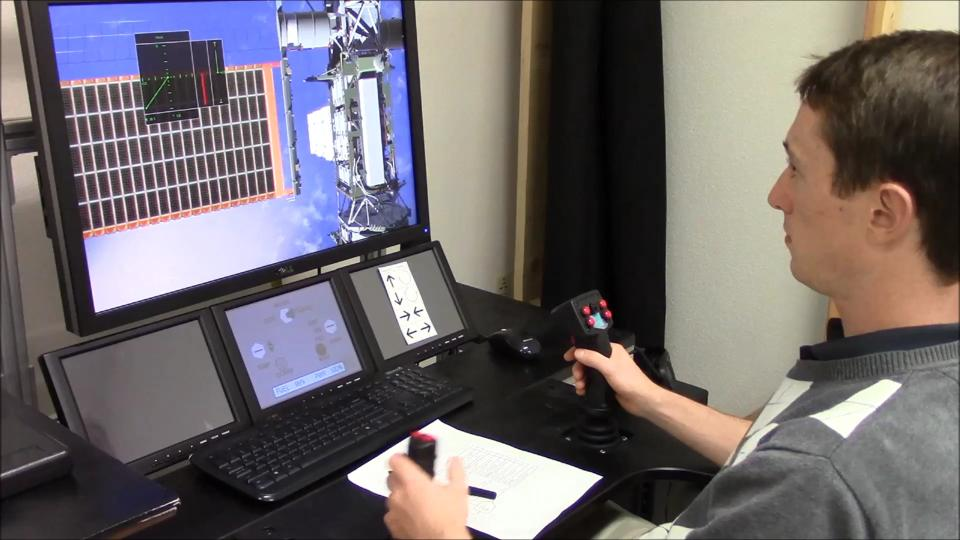
\includegraphics[width=0.8\linewidth]{figures/AR/SAFER_DangerChris.jpg}
        \caption[Simplified Aid for EVA Rescue (SAFER) experiment subject seated in the fixed-base simulator]{A subject from the Simplified Aid for EVA Rescue (SAFER) experiment seated in the fixed-base simulator~\citep{karasinski_real-time_2016}.}
        \label{figure:safersim}
    \end{center}
\end{figure}

Our recent work includes investigations into concurrent bandwidth feedback in a four degree of freedom Simplified Aid for EVA Rescue (SAFER) task~\citep{karasinski_real-time_2016, karasinski_real-time_2017, karasinski_development_2016}.
SAFER is a small propulsive jet pack worn during spacewalks for self-rescue~\citep{Vassigh1998}.
Subjects were tasked with flying a SAFER simulation to perform an inspection of the International Space Station's (ISS) solar arrays.
Subjects were initially placed 40 feet away from the solar array and were asked to close to 30 feet and hold this distance for the remainder of the task.
They could gauge their distance from the solar array using the indicator on the guidance display and the out-the-window display.
Subjects were then asked to inspect four waypoints on the solar array, and were given a guidance display for navigation to the waypoints.
Two vertically arranged displays in the simulator were available to complete the task (see Fig.~\ref{figure:safersim}).
The primary display contained an out-the-window view of the solar array and, depending on which group the subject was in, one of the guidance displays.
The secondary display located directly below the primary display portrayed information about the subject's current mode, remaining fuel, and a ``comm light''.

\begin{figure}[tb!]
    \begin{center}
        \begin{subfigure}{0.49\textwidth}
            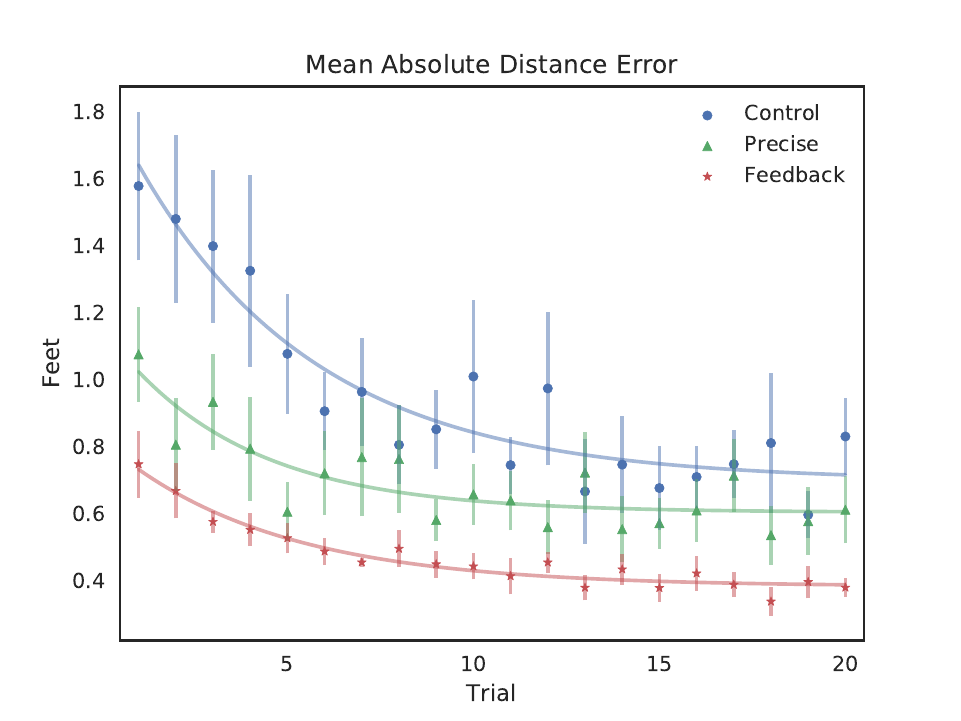
\includegraphics[width=\linewidth]{figures/AR/Group_absDistErr_clean_fit_30.png}
            \caption[Mean absolute distance error]{Mean absolute distance error, by group.}
            \label{figure:saferdistance}
        \end{subfigure}\hfill
        \begin{subfigure}{0.49\textwidth}
            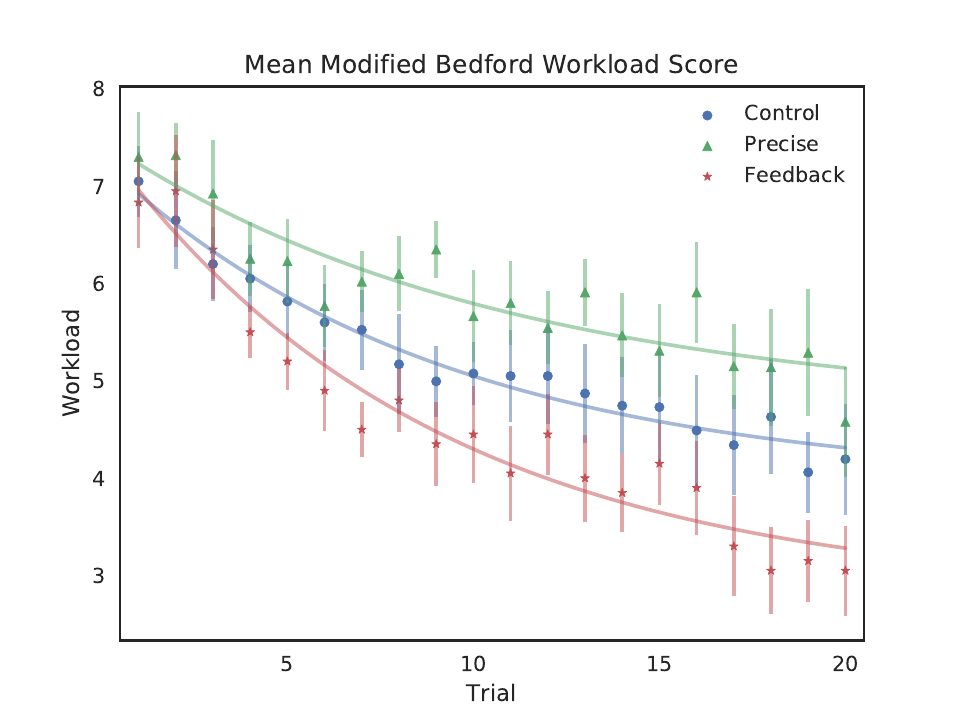
\includegraphics[width=\linewidth]{figures/AR/Group_Workload_fit_30.png}
            \caption[Mean subjective workload rating]{Mean subjective workload rating, by group.}
            \label{figure:saferworkload}
        \end{subfigure}
        \caption[Performance and workload benefits from feedback]{Subjects with concurrent bandwidth feedback (CBF) performed the best (a) and reported the lowest workload (b). Errors are the standard error of the mean~\citep{karasinski_real-time_2016}.}
    \end{center}
\end{figure}

In our experiment, subjects were placed into one of three groups: a control, a high precision augmented feedback group, and a concurrent bandwidth feedback (CBF) group.
Subjects in the high precision group were given an extra significant figure in their guidance display and an analog display which was scaled twice as large (but had half the maximum value) of their flight parameters.
Subjects in the CBF group had two display elements which would change from a green to a red color when the subject's performance was outside a predefined range.
Performance was measured as mean absolute distance error (MAE) and results across trials are shown in Fig.~\ref{figure:saferdistance}.
Both treatment groups performed better than the control group, with the CBF group performing the best and having the least error.
The effects that the treatments had on workload was very different than performance, however.
Subjects in the high precision group reported significantly more workload than the control group, while subjects in the CBF group reported significantly less workload than the control group (see Fig.~\ref{figure:saferworkload}).
The concurrent bandwidth feedback also had the added benefit of significantly reducing the amount of time required to train the subjects to their maximum skill level.
Subjects with the CBF performed better on their first trial than subjects in the control group did on their last, which was after approximately two hours on the task.

\subsubsection{Stereoscopic Displays}
Stereoscopic displays are systems ``in which two slightly different views of a scene are provided to a viewer, one image for each eye... allow[ing] the viewer's binocular visual system to extract depth information in a scene using this disparate information''~\citep{mcintire_stereoscopic_2014}.
Without the aid of the binocular depth cue presented by stereoscopic displays, viewers are instead entirely reliant on monocular clues such relative sizing, occlusion, and motion.
One of the primary motivation for stereoscopic displays is that ``[t]he visual scene of a 3D world is a more `natural,' `ecological,' or `compatible' representation than that provided by 2D displays''~\citep{wickens_three-dimensional_1990}.
As a result of this motivation, the effects of stereoscopic displays on human performance have been extensively studied in the literature.
Several authors have attempted to classify which types of tasks may stand to benefit~\citep{mcintire_stereoscopic_2014, wickens_three-dimensional_1990, wickens_three-dimensional_1989, naikar_perspective_1998, dixon_human_2009}.
A recent review of 184 papers, for example, suggests that 60\% of studies showed some benefit of 3D stereo displays, 15\% of tasks showed unclear or mixed benefits, and 25\% of studies showed no clear benefits~\citep{mcintire_stereoscopic_2014}.
In their review, tasks involving finding/identifying/classifying objects and tasks involving real/virtual spatial manipulations of objects benefited the most, while learning/training/planning tasks were the least likely to show a benefit.

Kim et al. also performed a quantitative evaluation of perspective and stereoscopic displays in a three-axis manual tracking task~\citep{kim_quantitative_1987}.
They investigated the differences between perspective and stereoscopic displays, the elevation angle, azimuth angle, and the effects of two visual enhancements: a grid and a reference line.
They found very strong relationships between elevation and azimuth angles and tracking performance, with the best performance occurring at an elevation angle of 45 degrees and an azimuth angle of 0 degrees.
Tracking performance decreased rapidly as the azimuth angle varied, and decreased less rapidly as the elevation angle varied.
In general, they found that the stereoscopic display allowed for better tracking performance, though the inclusion of the reference line visual enhancement greatly decreased the benefit over the perspective display.
Using only two subjects, they provided some insight into intrasubject and intersubject variability.
In several instances, intrasubject variability showed 50\% changes within the same experimental condition, while intersubject variability also appeared quite large in some conditions.
Kim et al. repeated the evaluation of these parameters on a telerobotics pick-and-place study~\citep{kim_visual_1987}.
They found similar results in this second study, suggesting that their results could be generalized and that three-axis tracking performance can be correlated with pick-and-place completion time.

Smallman at al. similarly investigated the effect of visual enhancements and 2D vs 3D displays for the development of a naval air warfare console~\citep{smallman_track_2000}.
Participants viewed naval and aircraft tracks in either a conventional 2D top-down display or a 3D display, and then attempted to reconstruct track positions.
They investigated the effectiveness of drop-lines and drop-shadows, and found that they significantly improved subjects ability to localize aircraft compared to when the enhancements were not present.
Furthermore, in the absence of either visual enhancement, subjects performed better with the 2D display than the 3D display.
Similar to Kim et al., they ultimately recommended that 3D stereoscopic displays include the use of a reference or drop-line for optimal performance.

\subsubsection{Workload Measurement}
Improving performance, through some kind of feedback or other technique, often comes at the cost of increased workload, which can lead to a loss of the ability to maintain performance.
Workload was defined by Hart and Staveland as ``the perceived relationship between the amount of mental processing capability or resources and the amount required by the task''~\citep{hart_development_1988}.
Having a low workload indicates that it would be easy to complete additional tasks, while having a high workload suggests that it would be difficult.

The NASA Task Load Index (NASA-TLX) is one of the most well known and commonly used subjective workload measures.
The NASA-TLX has been in use for thirty years, and has been used and validated over a large variety of tasks~\citep{hart_nasa-task_2006}.
The NASA-TLX is a multidimensional rating scale which uses the magnitude and ranking of six subscales to produce an overall estimate of subjective workload~\citep{hart_development_1988}.
The six subscales are: Mental Demand, Physical Demand, Temporal Demand, Performance, Effort, and Frustration.
Each of these scales is rated on a 0 (Very Low) to 100 (Very High) scale, with the exception of Performance, which is rated from 0 (Perfect) to 100 (Failure).
After marking a value for each of these subscales, subjects then make fifteen pairwise weightings, allowing them to rate each pair of subscales based on its perceived contribution to their overall workload.
A final, overall workload score is computed by multiplying each subscale's score by the number of times it was chosen in the pairwise weightings, adding these values, and dividing by fifteen.
As certain subscales may be more or less important than others, depending on the task being evaluated, some researchers can drop subscales or simply not compute the overall score.

In addition to subjective measures of workload, there are a variety of techniques which aim to estimate objective workload.
One of the most common objective measurement techniques is the secondary task, which requires subjects to complete the primary task, then use any spare workload to respond to an additional task~\citep{gawron_human_2008}.
Secondary tasks can provide a measure more sensitive to differences in workload and performance than a single task alone and allow for a common measure between experimental conditions~\citep{slocum1971meaningful}.
Care must be taken, however, to ensure that the secondary task does not intrude upon primary task performance~\citep{williges_behavioral_1979}.
In our previous studies, we have used a multiple choice reaction time task as an objective workload measurement.
In this secondary task, subjects are presented with several different stimuli, each of which requires a different response~\citep{lysaght_operator_1989}.
A subject's objective workload can then be inferred by either the percentage of secondary tasks which were correctly responded to within a given time, the number of secondary tasks which were correctly responded to in a trial, or both.
We have previously found this type of task to be correlated with subjective workload scales in the aforementioned SAFER task~\citep{karasinski_real-time_2017}.

\subsubsection{Summary}
Concurrent bandwidth feedback has been used in a large variety of motor control tasks, and has generally been found to improve performance.
Until recently, however, only simple tasks such as physical movements or basic pursuit tasks have been investigated.
More recent works, including the lane-keeping task by de Groot et al., and our previous work with the SAFER task, have indicated that concurrent bandwidth feedback can also be quite effective for complex tasks.
The decrease in required learning time, improved performance, and decreased workload seen in the SAFER task show that concurrent bandwidth feedback may prove to be most useful very early in training when subjects are first exposed to complex, highly dynamic tasks.
While visual concurrent bandwidth feedback has been used in a variety of tasks, no researchers have investigated its effects on a three-axis tracking task.

Despite extensive previous research, to the authors' knowledge there exists no study in the literature addressing human performance or workload changes in manual tracking tasks between traditional computer monitors and mobile, augmented reality headsets.
If operator performance while using augmented reality displays is improved--or at the very least, not degraded--then these devices could prove especially valuable in scenarios where it is impractical or otherwise difficult to provide a traditional computer interface.
There are a variety of robotics tasks, such as pick-and-place tasks, for which performance may be improved by allowing an operator the mobility to move and view the scene from whatever position is convenient at a given time.
Traditional robotics stations require the operator to remain in a single position, and typically only allow for several camera angles.
Mobile augmented reality displays allow the operator to take advantage of their ability to move through the environment, without needing to manage external cameras.

\section{Materials and Method}
\begin{figure}[b!]
    \begin{center}
        % Thanks
        % https://tex.stackexchange.com/questions/67573/tikz-shift-and-rotate-in-3d

        \newcommand{\rotateRPY}[3]% roll, pitch, yaw
        {   \pgfmathsetmacro{\rollangle}{#1}
            \pgfmathsetmacro{\pitchangle}{#2}
            \pgfmathsetmacro{\yawangle}{#3}

            % to what vector is the x unit vector transformed, and which 2D vector is this?
            \pgfmathsetmacro{\newxx}{cos(\yawangle)*cos(\pitchangle)}
            \pgfmathsetmacro{\newxy}{sin(\yawangle)*cos(\pitchangle)}
            \pgfmathsetmacro{\newxz}{-sin(\pitchangle)}
            \path (\newxx,\newxy,\newxz);
            \pgfgetlastxy{\nxx}{\nxy};

            % to what vector is the y unit vector transformed, and which 2D vector is this?
            \pgfmathsetmacro{\newyx}{cos(\yawangle)*sin(\pitchangle)*sin(\rollangle)-sin(\yawangle)*cos(\rollangle)}
            \pgfmathsetmacro{\newyy}{sin(\yawangle)*sin(\pitchangle)*sin(\rollangle)+ cos(\yawangle)*cos(\rollangle)}
            \pgfmathsetmacro{\newyz}{cos(\pitchangle)*sin(\rollangle)}
            \path (\newyx,\newyy,\newyz);
            \pgfgetlastxy{\nyx}{\nyy};

            % to what vector is the z unit vector transformed, and which 2D vector is this?
            \pgfmathsetmacro{\newzx}{cos(\yawangle)*sin(\pitchangle)*cos(\rollangle)+ sin(\yawangle)*sin(\rollangle)}
            \pgfmathsetmacro{\newzy}{sin(\yawangle)*sin(\pitchangle)*cos(\rollangle)-cos(\yawangle)*sin(\rollangle)}
            \pgfmathsetmacro{\newzz}{cos(\pitchangle)*cos(\rollangle)}
            \path (\newzx,\newzy,\newzz);
            \pgfgetlastxy{\nzx}{\nzy};
        }

        \tikzset{RPY/.style={x={(\nxx,\nxy)},y={(\nyx,\nyy)},z={(\nzx,\nzy)}}}

        \begin{tikzpicture}
            \draw[-] node at (3.5,0,0) {$x$} (-3,0,0) -- (3,0,0);
            \draw[-] node at (0,3.5/2,0) {$y$, {\color{red} $y\textprime$}} (0,-3/2,0) -- (0,3/2,0);
            \draw[-] node at (0,0,3.5) {$z$} (0,0,-3) -- (0,0,3);

            \rotateRPY{0}{-30}{0}
            \begin{scope}[draw=red, text=red,fill=red,densely dashed,RPY]
                \draw[-] node at (3.5,0,0) {$x\textprime$} (-3,0,0) -- (3,0,0);
                %\draw[-] node at (0,3.5,0) {} (0,0,0) -- (0,3,0);
                \draw[-] node at (0,0,3.5) {$z\textprime$} (0,0,-3) -- (0,0,3);
            \end{scope}
            \draw [->] (0:1.5) arc (0:-15:1.5);
            \draw[-] node at (1.7,-.2,0) {$\theta$};
        \end{tikzpicture}

        \caption[Perspective display of the coordinate frame for the tracking tasks]{Perspective display of the coordinate frame for the tracking tasks, with the $x$, $y$, and $z$ axes labeled. After rotating by $\theta$ around the y axis, the resulting reference frame of $x\textprime y\textprime z\textprime$ is also labeled.}
        \label{designdiagram}
    \end{center}
\end{figure}

In our experiment, subjects were responsible for simultaneously completing three primary tracking tasks and a two-choice secondary task.
Each axis of the tracking task was disturbed by a sum-of-sines, resulting in a random appearing signal that was difficult for the subjects to predict.
The two-choice task appeared on a screen next to the tracking task, and asked subjects to respond to either a ``LEFT'' or ``RIGHT'' command by pressing a button.
Subjects controlled the three-axes and responded to the two-choice task by using a Microsoft Xbox controller.
The subjects used the left joystick on the controller to control the $x$ and $y$ axes tracking tasks.
Subjects moved this joystick left and right to control the $x$ axis, and up and down to control the $y$ axis.
The subjects used the right joystick on the controller to control the $z$ axis.
Subjects moved this joystick up and down to control the $z$ axis.
See Fig.~\ref{designdiagram} for a visualization of the coordinate frame of the primary tracking task.
Subjects used the left and right triggers on the controller to respond to the two-choice task, using the left trigger to indicate ``LEFT'' on the two-choice task, and the right trigger to indicate ``RIGHT'' on the two-choice task.

\subsection{Hypotheses}
This study assessed the influence of display type (perspective vs. stereoscopic), relative display attitude (zero degrees vs. thirty degrees), and concurrent bandwidth feedback (with vs. without) on performance and workload.
Objective performance was measured using the root-mean-square error (RMSE) of the depth ($z$) axis.
Objective workload was measured using the response time to the secondary task, and subjective workload was measured using the NASA-TLX.
It was hypothesized that:
\begin{description}[align=left]
    \item [Hypothesis 1] Concurrent bandwidth feedback will improve performance in the depth ($z$) axis for both display types, and will decrease workload.
    \item [Hypothesis 2] Stereoscopic augmented reality displays improve performance in the depth ($z$) axis, but do not affect workload.
    \item [Hypothesis 3] Rotating the display improves performance in the depth ($z$) axis for both display types, and will decrease workload.
\end{description}

\subsection{Procedure}
A total of 24 subjects (19 males, 5 females) were recruited in accordance with the University of California, Davis Internal Review Board (IRB), and subjects were not compensated.
There were 12 subjects in the 2D group, and 12 subjects in the 3D group.
Subjects were students in the University of California, Davis, College of Engineering.
All participating subjects had normal vision (no colorblindness, eyesight correctable to 20/20 vision) and full motor control of their hands.

\begin{figure}[t!]
    \begin{center}
        \begin{subfigure}{0.49\textwidth}
            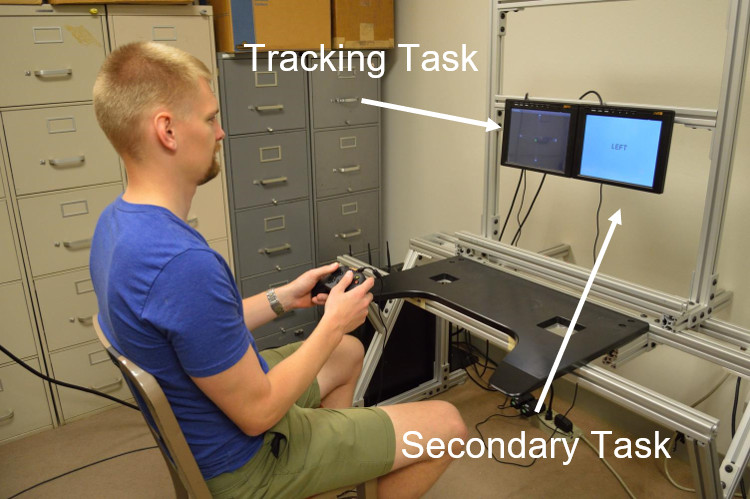
\includegraphics[width=\linewidth]{figures/AR/DSC_0801.JPG}
            \caption[2D Group]{2D Group.}
        \end{subfigure}\hfill
        \begin{subfigure}{0.49\textwidth}
            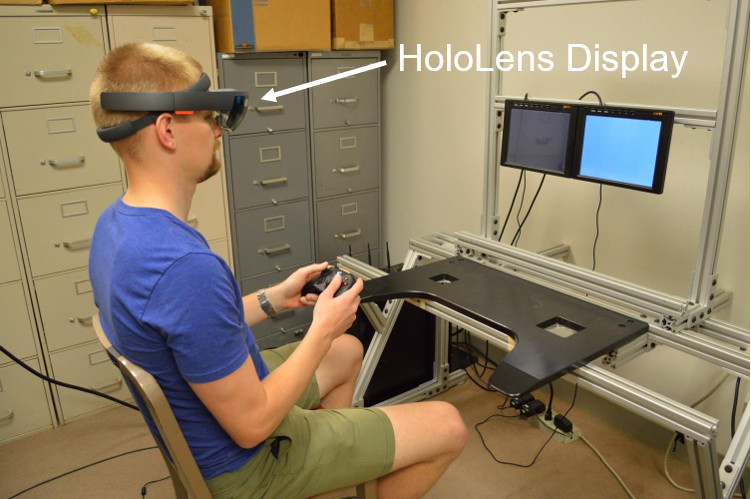
\includegraphics[width=\linewidth]{figures/AR/DSC_0803.JPG}
            \caption[3D Group]{3D Group.}
        \end{subfigure}
        \caption[The fixed-based simulator used by both groups]{The fixed-based simulator used by both groups.}%
        \label{fig:simulator}%
    \end{center}
\end{figure}

\begin{figure}[t!]
    \begin{center}
        \begin{subfigure}{0.32\textwidth}
            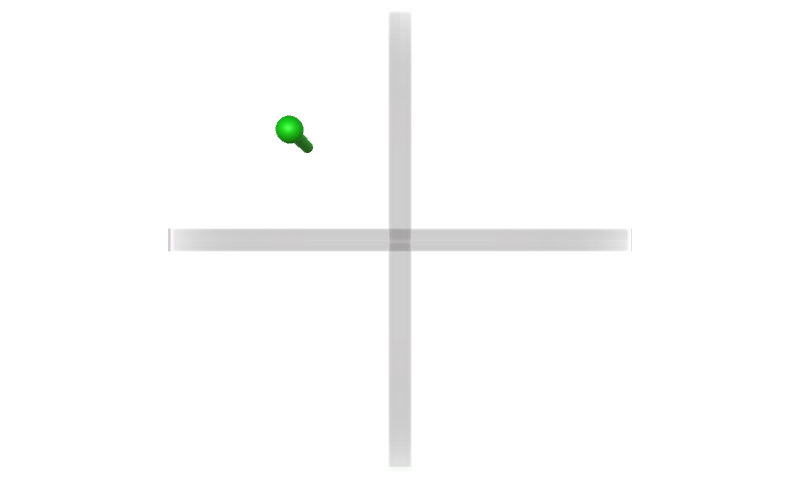
\includegraphics[trim={5cm 0 5cm 0},clip,width=\linewidth]{figures/AR/Baseline.png}
            \caption[Baseline]{Baseline.}
            \label{fig:designs_baseline}
        \end{subfigure}\hfill
        \begin{subfigure}{0.32\textwidth}
            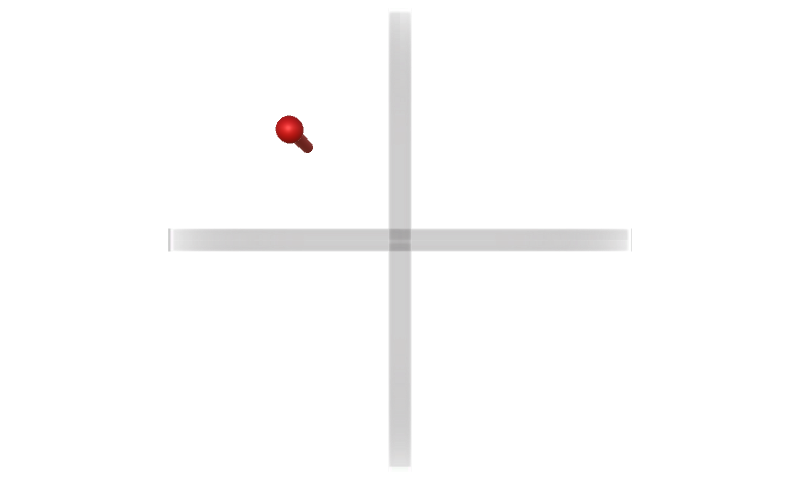
\includegraphics[trim={5cm 0 5cm 0},clip,width=\linewidth]{figures/AR/Color.png}
            \caption[Color Feedback]{Color Feedback.}
            \label{fig:designs_feedback}
        \end{subfigure}\hfill
        \begin{subfigure}{0.32\textwidth}
            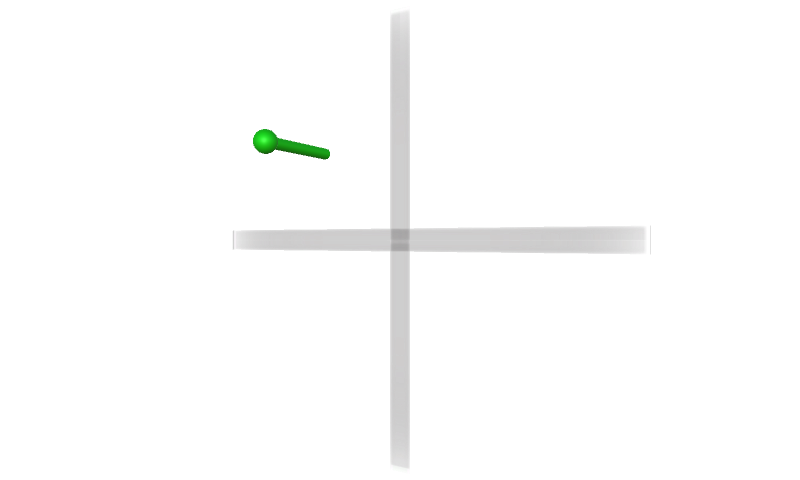
\includegraphics[trim={5cm 0 5cm 0},clip,width=\linewidth]{figures/AR/Angled.png}
            \caption[Rotated (about the $y$ axis)]{Rotated (about the $y$ axis).}
            \label{fig:designs_rotated}
        \end{subfigure}
        \caption[The three different designs in the same error state]{The three different designs in the same error state.
            (b) The color feedback has been activated here, changing the guidance target from green to red.}
        \label{fig:designs}%
    \end{center}
\end{figure}

A human-in-the-loop simulation was conducted using a fixed-base simulator (see Fig.~\ref{fig:simulator}).
The simulator consisted of two 10.4 inch LCD displays.
The primary tracking task was shown on the left display, while the right display showed the two-choice secondary task.
Subjects were seated for the duration of the experiment and were placed one meter perpendicular from the center of the left display.
For subjects in the 3D group, the left LCD monitor was turned off, and the tracking task was instead displayed on the HoloLens.
For these subjects, the cross was placed at the same height as the subject's head, such that it was viewed with no relative attitude in the baseline condition (see Fig.~\ref{fig:designs}).
Both groups viewed the guidance cross with a width and height of 5 inches by 5 inches.
For subjects in the HoloLen's group, the $z$ motion of the cross also could move up to 5 inches in either direction away from the center of the guidance cross.
Subjects in both groups used the same Microsoft Xbox controller and control scheme to complete the task.

The disturbance function was a sum of 13 sinusoids approximating a rectangular spectrum with a 2.0 rad/s cutoff frequency.
The disturbing force, as a function of time, $d(t)$, was
\begin{align}
    d(t) = \sum_{i=1}^{13} A_i \sin \left( w_i t + \phi_i \right)
    \label{eq:disturbance}
\end{align}
Each sine wave amplitude, frequency, and phase offset was borrowed from a similar experiment~\citep{hess_effects_1984}.
Table~\ref{sine-table} lists the sine wave amplitude, frequency, number of cycles in a 60 second run, and phase offset for each sine wave in the disturbance force.
This disturbance was the same for all subjects and trials, though the subjects were naive to this.
The $x$, $y$, and $z$ axes all experienced the same disturbance force generating function, but the $y$ axis was temporally offset by 60 seconds and the $z$ axis was offset by 120 seconds.
This allowed for a very similar generation of disturbance forces for each axis.
The RMSE of the disturbance force was normalized along each axis such that all three were the same.

\begin{table}[tb]
    \centering
    \includetable{3dar-sine-table.tex}
    \caption[Disturbance force characteristics]{The relative amplitude, frequency, number of cycles in each 60 second run, and phase offset each $i^{th}$ sine, see Equation~\ref{eq:disturbance}.}
    \label{sine-table}
\end{table}

\begin{table}[tb]
    \centering
    \includetable{3dar-designs.tex}
    \caption[The factors that were modified between the different designs]{The factors that were modified between the different designs.}
    \label{tab:designs}
\end{table}

Three designs were presented to the subjects to evaluate: a baseline design, a color-based concurrent bandwidth feedback (CBF) design, and a rotated design.
Fig.~\ref{fig:designs} shows all three designs in the same error state.
The three designs were very similar, having only minor differences between each other.

The baseline design consists of a flat cross with a center target point and a green sphere error indicator.
This indicator also casts a green, variable-length rod perpendicular to the plane of the cross, which allows for a visual estimation of the error in the $z$ axis.
The $x$ axis is parallel with the horizontal cross, while the $y$ axis is parallel with the vertical cross.
The color feedback design was identical to the baseline design in every way, with the addition of visual concurrent bandwidth feedback (green or red) on the $z$ axis.
When the absolute value of the error on the $z$ axis exceeded a fixed bandwidth, the color of both the spherical indicator and the cylindrical rod changed from green to red (see Fig.~\ref{fig:designs_feedback}).
When the absolute value of the error on the $z$ axis was lowered back below this fixed bandwidth, the indicator changed back to a green color (see Fig.~\ref{fig:designs_baseline}).
The rotated design was identical to the baseline design, but the relative attitude of the display was rotated about the $y$ axis by 30 degrees (see Fig.~\ref{designdiagram}).
This design was created to provide subjects with more visual variation in the $z$ axis, and 30 degrees was chosen after a brief pilot study.

Before entering the study, subjects were randomly placed in a display group (either the LCD monitor or HoloLens), and were then randomly placed into an order group (which consisted of Baseline-Feedback-Rotated, Feedback-Rotated-Baseline, and Rotated-Baseline-Feedback).
This order group was created to remove any order effects that might arise due to training on a given display, and follows a standard Latin squares design.
(The order of the designs was expected to be insignificant, but we will later discuss how this is not the case.)
After entering the experiment room, the subjects were familiarized with the task, three designs, NASA-TLX, and the controller through a twenty minute training session during which they were instructed to:
\begin{itemize}
    \item Minimize the displacement of their guidance target from the center
    \item Respond to the two choice task as accurately and quickly as possible
\end{itemize}

Subjects in the 3D group completed a short calibration program that adjusted the display to their interpupillary distance.
All subjects were then allowed to complete two familiarization trials, during which time they could ask questions about how the controls worked, or any other aspects of the task.
The proctor also used this time to ensure that subjects showed basic competency with the task by responding to both the tracking and two-choice tasks appropriately.
All familiarizations were done with the baseline design, regardless of which design the subjects evaluated first.

After this familiarization process, subjects completed ten trials with their first design.
After completing these trials, they answered a brief survey which asked them if the design was adequate to complete the task.
Subjects were also asked to subjectively rate their performance in a questionnaire after evaluating each design.
Subjects were asked to rate ``I found the tracking display adequate to complete the task.'' on a five point scale where 1 indicated ``Strongly Disagree'' and 5 indicated ``Strongly Agree''.
After this survey, subjects then completed a NASA-TLX workload survey.
Subjects then repeated this process with their second and third designs.
At the conclusion of the three designs, subjects were also asked to complete a preference survey which inquired into what design the subjects preferred.

\section{Results}
We conducted three-way mixed ANOVAs between display (2D or 3D), design (Baseline, Feedback, or Rotated), and starting design (Baseline, Feedback, or Rotated) with repeated measures on the design factor.
When significant effects were observed, post hoc comparisons using the Tukey Honest Significance Difference (HSD) test with a Bonferroni adjustment were completed to investigate which pairs of the factor were significant.
In order to remove learning and fatigue effects, each subject's best performing five trials in each design were averaged together to produce one average score for each subject and design.
Additionally, the first ten seconds of each sixty second trial were not included in the analysis to remove initial transient effects.

The root-mean-square error (RMSE) of the depth ($z$) axis was used to understand the differences between the three designs and the two devices.
The RMS of the disturbance signal was calculated and used to normalize the RMSE.
Under this definition, an RMSE of 1 indicates performance no better than no input, and an RMSE greater than 1 indicates quite poor performance.
It was expected that the baseline design would lead to the worst performance in the $z$ axis than the color feedback and rotated designs.
It was also expected that, due to the stereoscopic nature of the display, the HoloLens would allow for better performance than the 2D LCD monitor along $z$ axis.

\begin{figure}[tb!]
    \begin{center}
        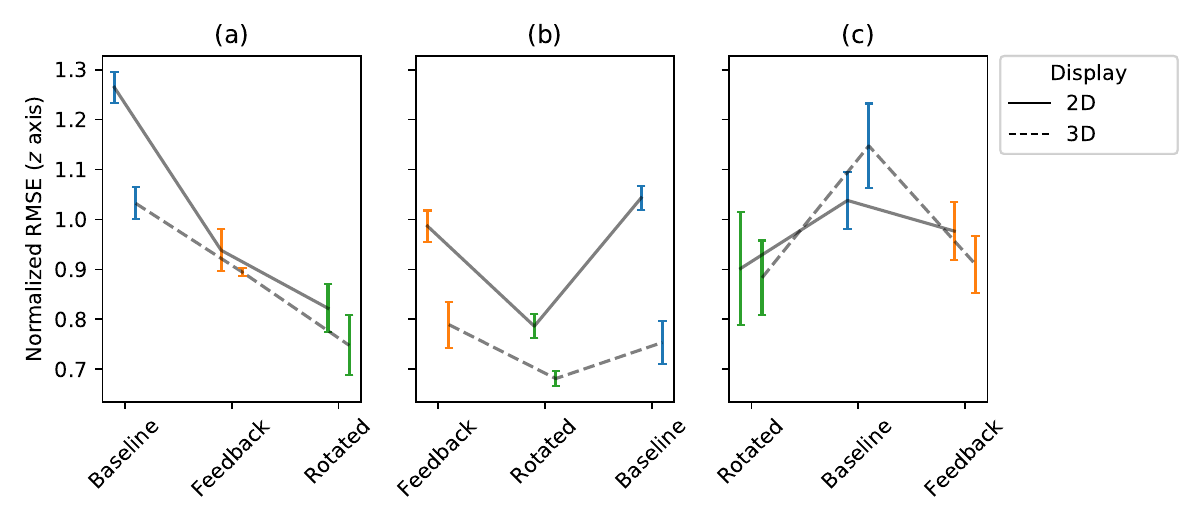
\includegraphics[height=7cm]{figures/AR/x_design_y_zrmse_col_startdesign_hue_device.png}
        \caption[The resulting normalized RMSE along the $z$ axis]{The resulting normalized RMSE along the $z$ axis. Subjects started in either the (a) Baseline, (b) Feedback, or (c) Rotated design.}
        \label{fig:zrmseanovas}
    \end{center}
\end{figure}

Results of the ANOVA on the $z$ axis RMSE showed significant effects for design ($F(2, 36)=84.92, p<.001$), device ($F(1, 18)=7.22, p<0.015$), and start design ($F(2, 18)=4.81, p<0.021$).
The ANOVA also showed a significant interaction effect between design and starting design ($F(4, 36)=8.55, p<0.0001$), and a three way interaction between design, device, and starting design ($F(4, 36)=5.57, p<0.002$).
Further investigation into the effect of starting design using pairwise comparisons showed significance differences between subjects that started in the concurrent bandwidth feedback group and those in the baseline ($p<0.001$) or rotated ($p<0.001$) designs, but no difference between subjects that started in the baseline and rotated designs ($p>.38$).
The difference in performance between design, device, and starting design can be seen in Fig.~\ref{fig:zrmseanovas}.

Due to the unanticipated but significant interaction effects in the starting design factor, the remainder of the analysis is split between subjects who started with the concurrent bandwidth feedback design and those that did not (e.g., those that started in the baseline or rotated design).
For subjects that started in the CBF design, there was a significant effect of design ($F(2, 12)=21.65, p<.0001$), a significant effect of display ($F(1, 6)=36.73, p<0.001$), and a significant interaction effect between design and device ($F(2, 12)=5.42, p<0.021$).
For subjects that did not start in the CBF design, there was a significant effect of design ($F(2, 28)=38.70, p<.0001$), but no significant effect or display ($F(1, 14)=1.03, p>0.32$), and no interaction effect ($F(2, 12)=0.03, p>0.97$).
The resulting difference between subjects who started in the CBF design and those who did not is presented in Fig.~\ref{fig:zrmseanovas2}.
For subjects who did not start in the CBF design, display had no significant effect, and subjects performed best in the rotated design, followed by the feedback design and finally the baseline design.
Subjects who started in the CBF design performed significantly better in the 3D display than the 2D displays, and performed best in the rotated design, but comparably between the feedback and baseline designs.

\begin{figure}[tb!]
    \begin{center}
        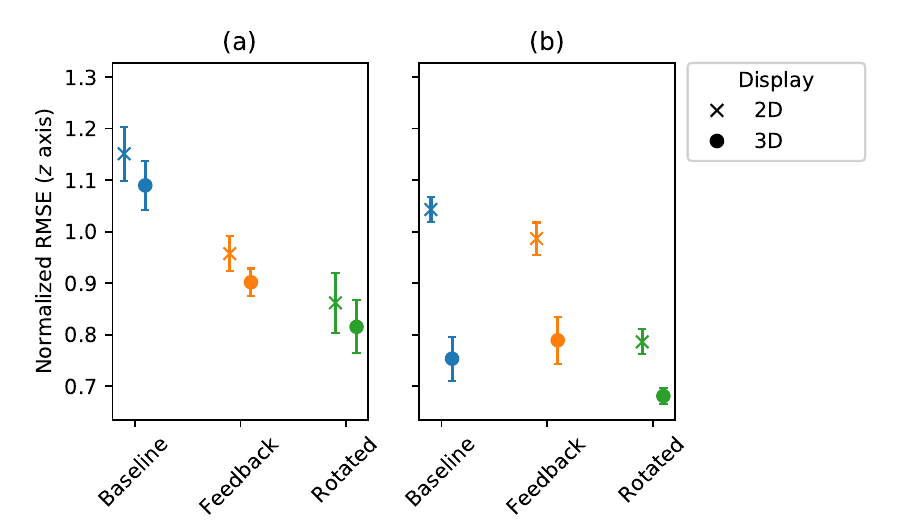
\includegraphics[height=7cm]{figures/AR/x_design_y_zrmse_hue_device_col_cbf_first.png}
        \caption[The resulting normalized RMSE along the $z$ axis]{The resulting normalized RMSE along the $z$ axis, grouping by subjects that started (a) without or (b) with feedback.}
        \label{fig:zrmseanovas2}
    \end{center}
\end{figure}

The NASA-TLX was used to measure differences in subjective workload, and the reaction time to the secondary task was used to measure differences in objective workload between design, device, and starting design.
There were no significant effects, nor interaction effects, found in the ANOVA for design, device, or starting design for the NASA-TLX measurements.
There was a significant effect of design ($F(2, 36)=7.93, p<0.0014$) for the reaction time to the secondary task, though the magnitude of this effect was very small between designs (less than 100 ms difference) and was not significant during Tukey HSD tests.
In general, there were no significant effects found for workload measurements.

\section{Discussions and Conclusion}
To summarize these results, there were significant effects found in the $z$ axis RMSE for design, with subjects generally performing the best using the rotated design, followed by the CBF design, and performing worst with the baseline design.
There were significant effects found for the factors of device and starting design, though these must be interpreted carefully.
Subjects who started with concurrent bandwidth feedback performed better than subjects who did not.
We believe that this result reinforces that found in our prior SAFER experiment, where subjects who were exposed to the CBF early on learned the task better than those who were not exposed~\citep{karasinski_real-time_2017,karasinski_development_2016,karasinski_real-time_2016}.
An interesting effect of this exposure is that, after learning the task with CBF, subjects continued on to perform significantly better in the baseline condition than those subjects that did not start in the CBF design.

Subjects who started in the CBF design and who were wearing the HoloLens appear to have used the CBF to better learn the depth cue presented in the stereoscopic display.
These subjects continued to perform significantly better than subjects who started with the CBF design but without the stereoscopic display when they continued to the baseline design.
This indicates that even a brief exposure to the concurrent bandwidth feedback was sufficient to induce improved performance in the baseline design.
Additionally, this also suggests that well trained subjects could perform better using the stereoscopic display compared with the traditional display, but that subjects who were still learning the task could not take advantage of the additional depth cues provided by the display.
Finally, there were no significant effects found for the NASA-TLX measurements, and there were significant but small effects found between the designs for reaction time.

In summary, we find partial agreement with all of our hypotheses in respect to the performance aspects of our experiment, while the workload was essentially unaffected by all of our experimental factors.
For Hypothesis 1, subjects who completed the baseline design before the CBF design performed better in the CBF design, while subjects who completed the CBF design before the baseline performed approximately the same in both designs.
This indicates that CBF can both improve performance compared to a baseline design, and better train subjects such that, even after brief exposure, the feedback is no longer required.
Workload was unaffected by the CBF.
For Hypothesis 2, subjects who started in the CBF design appear to have better learned the task and used the CBF to learn to interpret the depth cue provided by the stereoscopic display.
Subjects who were not initially exposed to this feedback were unable to exploit the display, and did not perform significantly better than subjects without the display.
For Hypothesis 3, subjects in the rotated design did perform better than those in the baseline design and appeared to be able to use this view to better interpret the depth of the target.

These results suggest that 3D displays such as the HoloLens have the potential to improve performance, but that simply donning a 3D display is not in itself wholly sufficient for improvement.
Subjects performed the tracking task better when we exposed them to CBF early in the experiment, and were able to use the depth cues provided by the 3D display to sustain this improvement when the feedback was removed.
These subjects achieved the best performance that we observed in this experiment, suggesting that the combination of CBF and 3D displays is an effective training technique for optimal performance.
The rotated design generally resulted in excellent performance by all subjects, which suggests that a direct ($\theta=0$) view should be avoided for three-axis tracking tasks.
Care must be taken to provide subjects with the feedback required to adequately complete the task, and subjects should not expect to perform better simply because they have 3D displays.

% \section*{Acknowledgments}
% The authors would like to thank all the subjects for volunteering to take part in the study.
% This work was supported by the Link Foundation's Modeling, Simulation, and Training Fellowship.

\chapter{Surface Electromyography Task}
\label{chap:emg}

The previous Chapter shows the benefits of applying concurrent bandwidth feedback to continuous motor control, but did not explore if this feedback can be successfully applied to more discrete tasks.
To further investigate the utility of concurrent bandwidth feedback, we applied it to an electromyography-based control task.
This experiment also investigated the difference between using concurrent and terminal feedback as potential training strategies to reduce the required time to use electromyography control.
Portions of this chapter were originally published in the conference proceedings for AIAA SciTech 2020 \citep{doi:10.2514/6.2020-1110}.

% \title{The Effects of Training Methodology on Performance, Workload, and Trust During Human Learning of a Computer-Based Task}

% \author{Sarah M. O'Meara\footnote{Graduate Student Researcher, Mechanical and Aerospace Engineering Department.} and John A. Karasinski\footnote{Graduate Student Researcher, Mechanical and Aerospace Engineering Department, Student Member AIAA.} and Casey L. Miller\footnote{Research Assistant, Mechanical and Aerospace Engineering Department.} and Sanjay S. Joshi\footnote{Director, Robotics, Autonomous Systems, and Controls Laboratory, Professor, Mechanical and Aerospace Engineering Department.} and Stephen K. Robinson\footnote{Principal Investigator, Human/Robotics/Vehicle Integration and Performance Lab, Professor, Mechanical and Aerospace Engineering Department, Associate Fellow AIAA.}}
% \affil{University of California, Davis, Davis, CA, 95616, USA}

\section{Introduction}
% Biophysical monitoring during aviation operations has recently gained increased interest as a safety feature and a means to create an adaptive cockpit.
% Safety-related concerns include cognitive workload~\citep{RN1, RN2}, muscle strain~\citep{RN3, RN4, RN5}, and security~\citep{RN6}.
% Pilots may develop inattentional deafness to auditory alarms, but biophysical monitoring has the potential to predict these occurrences~\citep{RN7}, discriminate between cognitive loads~\citep{RN1}, and predict cognitive fatigue which results in missed auditory targets~\citep{RN2}.
% The potential causes of muscle fatigue and strain has also been studied in helicopter pilots~\citep{RN3, RN4, RN5}, as well as electromyography (EMG) measurement accuracy~\citep{RN8}.
% EMG has been used in aviation research to predict and warn pilots of G-Induced Loss of Consciousness~\citep{RN9, RN10}, to discriminate between novice and experienced pilots~\citep{RN11}, to control forces during emergency maneuvers~\citep{RN12}, and to command pitch and bank rates of an aircraft simulation~\citep{RN13}.

% More recently, incorporating biophysical measurements has been suggested for UAV operation~\citep{RN14}.
% EMG control has also been applied to robotics~\citep{RN15, RN16, RN17, RN18} with potential aerospace applications, such as tele-operations~\citep{RN19}.
% In addition to tele-operations control~\citep{RN20, RN21}, EMG inputs have been used to modulate robotic arm stiffness for more precise tasks~\citep{RN22, RN23}.
% While these studies have developed control strategies, they have not addressed the training aspect which is essential for the critical and complex environments found in aerospace operations.
% Development of more sophisticated and integrated human-automation interfaces is clearly a trend in aviation, and more broadly in aerospace as a whole.

% \subsection{Selected Training Methodologies}
Training novice users to effectively use electromyography (EMG) control can be a long and difficult task~\citep{RN24}.
EMG control has been applied to robotics~\citep{RN15, RN16, RN17, RN18} and tele-operations~\citep{RN19}, and has been suggested for UAV operation~\citep{RN14}, but long learning times have generally prevented EMG from being used operationally.
The use of augmented feedback strategies, however, have been shown to help reduce training times.
Augmented feedback provides information that ``cannot be elaborated without an external source; thus, it is provided by a trainer or a display'' and has been shown to effectively improve performance in a wide variety of motor tasks~\citep{sigrist_augmented_2013}.
Biofeedback, which applies augmented feedback strategies to physiological signals such as EMG, has proven to be a useful tool for improving performance and assisting in rehabilitation~\citep{RN26}.
Researchers have investigated various augmented biofeedback techniques and have found them to help subjects to ``become more cognizant of their own EMG signal'', allowing for better control~\citep{RN27}.
A recent review of the biofeedback literature suggests that ``[b]iofeedback is more effective than usual therapy,'' though they also note that ``[f]urther research is required to determine the long-term effect [biofeedback has] on learning''~\citep{RN28}.

Augmented feedback can be split into two large categories describing when the feedback is presented to a subject.
Concurrent feedback is presented in real-time, as subjects complete a task, while terminal feedback is presented after the task is complete.
In general, concurrent feedback has been shown to be more useful with increasing functional task complexity, while terminal feedback is often less useful when complexity is high~\citep{sigrist_augmented_2013}.
Concurrent feedback has recently shown great promise in EMG control, though less progress has been made comparing the effects of terminal feedback strategies or investigating long-term learning effects~\citep{RN29, RN30, RN31, RN32}.

Additionally, research into the bayesian theory of motor adaptation, which suggests that increased errors and decreased visual uncertainty lead to faster adaptation, may be a useful training methodology for reducing training times.
Research into motor adaptation and surface EMG (sEMG) control has showed great promise compared to traditional techniques~\citep{RN33}.
Recent research at UC Davis has further investigated the use of motor adaptation for two-dimensional myoelectric control~\citep{RN35}.
\citeauthor{RN35} found that subjects were more successful at hitting targets when exposed to control perturbations compared to a control group, and concluded by suggesting that ``exposure to a variable mapping encourages exploratory behavior and underlies a change in adaption rate, which could potentially be used to train myoelectric control users.''
Motor adaptation has not previously been used as a training methodology, however, and it is unclear how it would compare to an augmented feedback based methodology.

\subsection{Trust in Automation}
Trust is an important factor when considering human-automation interaction, and inappropriate trust can lead to the disuse or misuse of automated systems.
Trust is ``the attitude that an agent will help achieve an individual's goals in a situation characterized by uncertainty and vulnerability''~\citep{lee_trust_2004}.
The reliability of a system, in particular, has been shown to be an important aspect of an operator's trust in a system~\citep{RN38}.
While there have been many proposed models for trust, \citeauthor{RN39}'s three layer model deserves particular attention.
After performing a systematic review of the literature, they developed a three-layer model of trust which is split between dispositional trust, situational trust, and learned trust.
Though researchers have little control over dispositional trust, they can affect situational trust by varying an experimental interface or environment and learned trust can be evaluated using repeated measures.

\subsection{Summary}
% Our recent work at University of California (U.C.), Davis includes three studies which have shown that concurrent feedback techniques can improve performance and have the potential to reduce cognitive workload in especially demanding tasks.
% We investigated the effects of concurrent feedback in a simulated, four degree of freedom manually-controlled spacecraft inspection task~\citep{karasinski_real-time_2017}.
% Subjects in a feedback group performed the task much faster and more accurately than those in a control group and reported a significantly lower workload.
% We also investigated the effects of concurrent feedback on performance in a three-axis manual tracking task~\citep{karasinski_evaluating_2019}.
% We found that subjects could use concurrent visual feedback to better learn the depth cues provided by an augmented reality headset.
% Subjects were able to retain their performance improvement when the feedback was removed.
% Finally, we investigated the effects of using concurrent feedback to train an aircraft flight task with variable modes of difficulty~\citep{RN42}.
% Subjects exposed to the feedback immediately performed significantly better in every aspect of the task, continued this trend through the study, and retained these performance benefits after the feedback was removed in retention trials.

In this study, we address the effects of training methodology on performance, workload, and trust during a computer-based Fitts's Law cursor-to-target task~\citep{RN43}.
The training methodologies evaluated were concurrent and terminal augmented feedback and motor adaptation based on variable mapping of control inputs.
To test if the benefits provided by these training methodologies were acting to improve learning or simply being used as performance enhancers when present, we removed the feedback and variable mapping at the end of the study.

\section{Materials and Methods}
\subsection{Subjects and Experimental Setup}

55 subjects were recruited from the University of California, Davis's Psychology department.
Subjects were excluded if they had a history of neuromuscular disorders, physical limitations of dominant arm, or prior sEMG control experience.
Of the 55 subjects recruited, 48 completed the complete protocol and had an average age of 20.07 years (SD = 1.39).
This study was approved by the University of California, Davis Institutional Review Board (Project \#1461183-1), and subjects provided written consent and were compensated in the form of university research credits.

The experimental setup for attaching the electrodes for the EMG control followed \citeauthor{RN44}, and two electrodes (ConMed 1620 Ag/AgCl center snap) approximately 2.5 cm apart were placed on the dominant hand side near the extensor digitorum proximal attachment.
The signal from the electrodes was acquired as described in \citet{RN44}, and the signal processing followed \citet{RN45}.
The raw signal was windowed, and the root-mean-square (RMS) value for each window was calculated, normalized by a manually set calibration constant, and incorporated into a moving average window to yield $\bar{x}$, see Equation~\ref{eq:emgvelocity}.

\subsection{Experimental Design and Subject Groups}

Subjects in the experiment used EMG to control the cursor in a 2D center-out Fitts's Law task.
The task took place in a normalized area of -1 to 1 units in each direction.
To control the cursor, subjects input a series of three pulsive EMG commands which indicated a direction and velocity of the cursor.
For the pulse to be registered by the system, it needed to cross threshold value, $l_1$, which was nominally set to 0.20.
The first two pulses were each classified as ``short'' or ``long'', where long was indicated by holding the pulse for greater than 0.5 seconds, and different combinations of these pulses formed a 2-bit code.
The different codes represented up, down, left, and right, and two ``short'' pulses, for example, selected the up command.
After the first two pulses were entered and recognized as a movement code, the third pulse could be used to command the velocity of the cursor.
The cursor velocity was defined by Equation~\ref{eq:emgvelocity},
\begin{equation}
	\label{eq:emgvelocity}
	v= v_c+\left(v_m-v_c\right)\left[\frac{\left(\bar{x}-l_2\right)}{\left(1-l_2\right)}\right]
\end{equation}
where $v_c$ was the minimum velocity (0.05 units/second), $v_m$ was the maximum velocity (0.50 units/second), $l_2$ was 0.30, and $\bar{x}$ was the filtered, averaged sEMG input.
The interface and this control strategy was first presented in \citet{RN45}, and further pilot studies were conducted to determine a maximum time of 60 seconds for subjects to complete a Trial.

Subjects were randomly assigned to one of four groups (12 subjects per group), and each was exposed to separate training methodology:
\begin{enumerate}
	\item The Control group trained solely through repetition.
	\item The Concurrent Feedback group received visual feedback during the task which indicated when the sEMG signal exceeded the threshold value, $l_1$, for selecting commands.
	\item The Terminal Feedback group received visual feedback during the task after they successfully entered a command.
	\item The Adaptive Threshold group was the same as the Control group, but the threshold value, $l_1$, varied Trial-to-Trial and was randomly selected for each Trial ($l_1 = 0.10, 0.15, 0.20, 0.25, 0.30$).
\end{enumerate}
Despite the presence of visual feedback, the Concurrent and Terminal feedback groups viewed very similar interfaces to that of the Control Group, see Figure~\ref{figure:label2}.
The Concurrent Feedback group's feedback appeared on the cursor itself (see Figure~\ref{figure:label2}b), while the Terminal Feedback group saw their visual feedback appear on the edge of the screen in the direction they commanded (see Figure~\ref{figure:label2}c).
An illustration of a potential signal input over time, along with an example of the feedback that would be presented for the two augmented feedback groups, is available in Figure~\ref{figure:label1}.

\begin{figure}[b!]
	\centering
	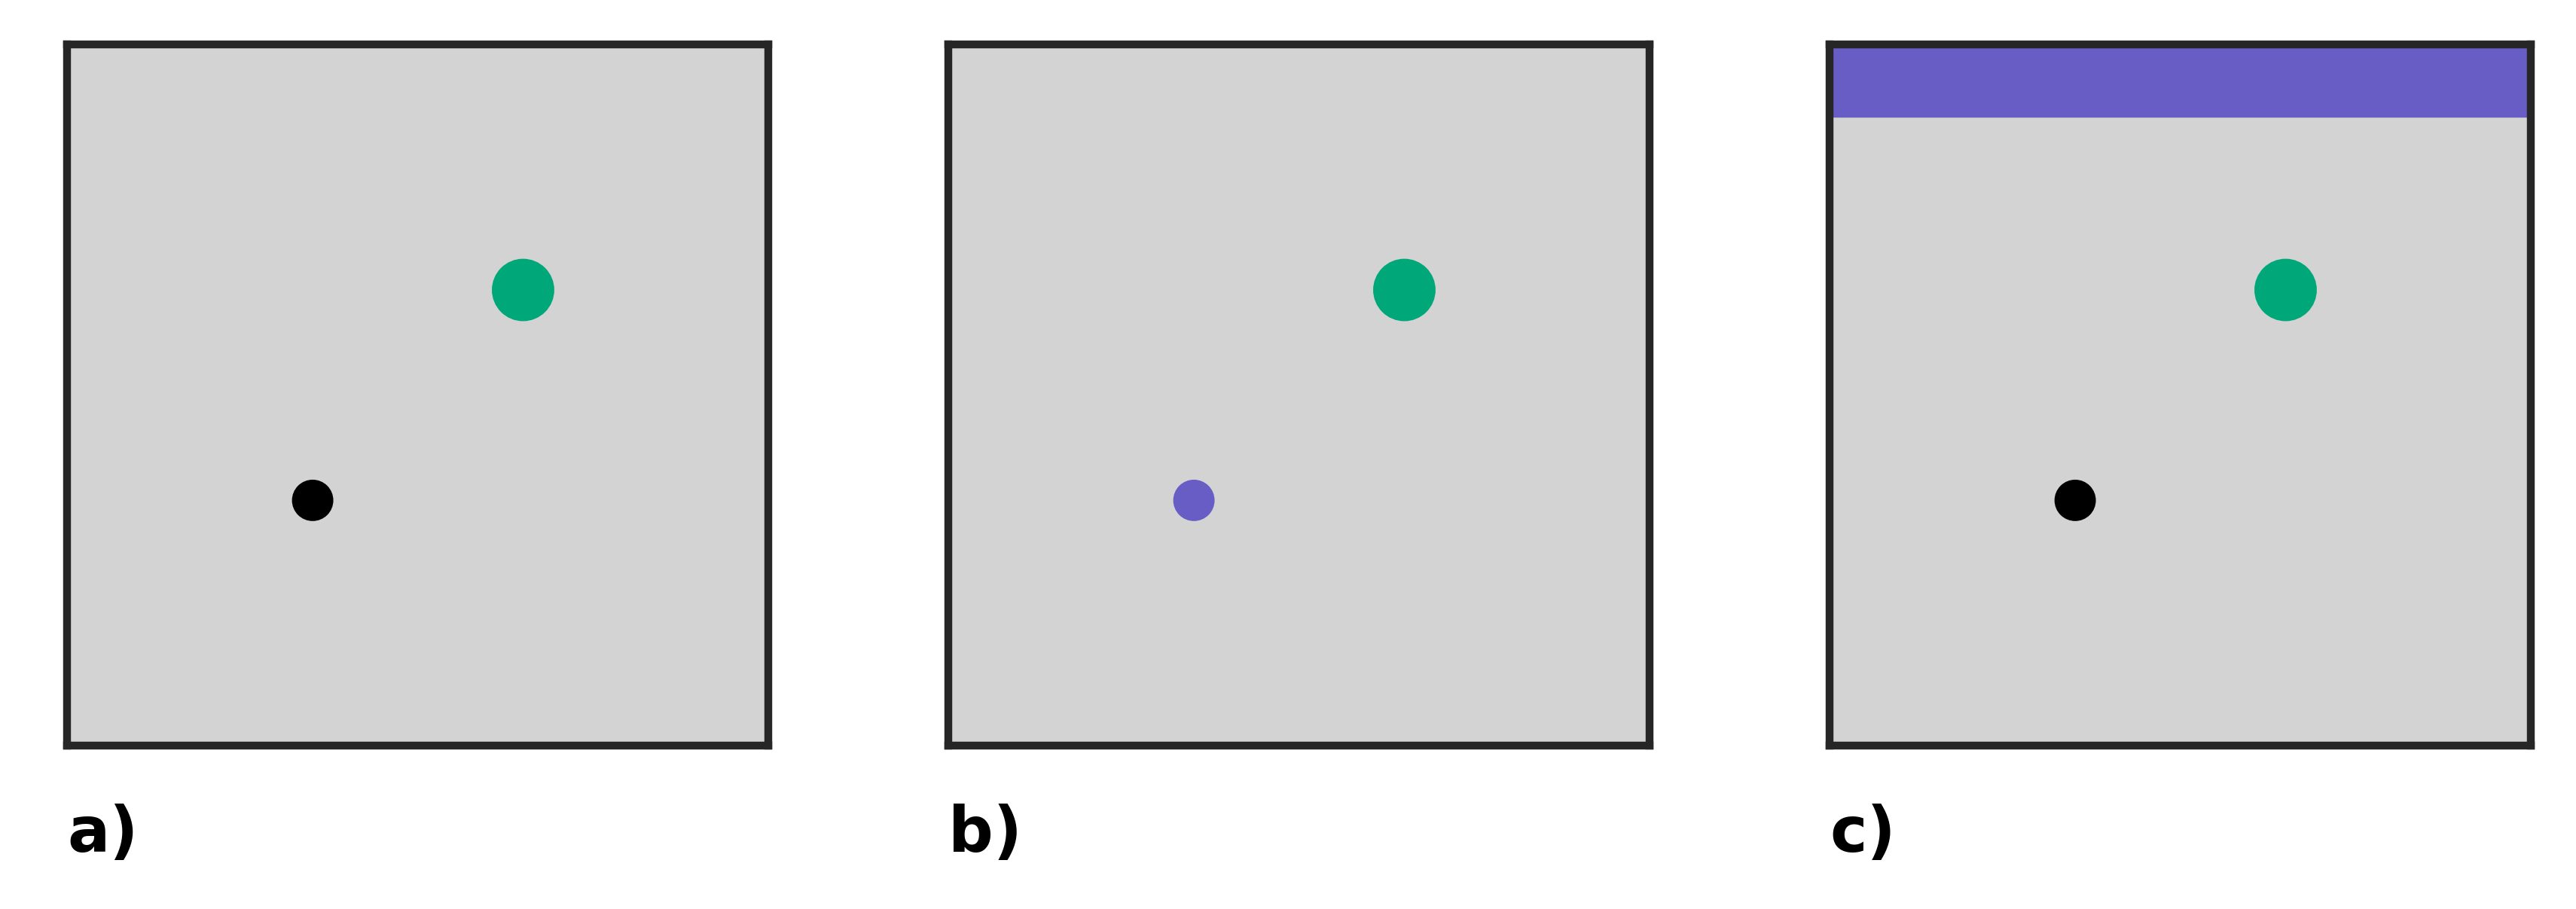
\includegraphics[width=.6125\textwidth]{figures/EMG/Figure2}
	\caption[Cursor interfaces]{Cursor interfaces for a) the Control and Adaptive Threshold, b) Concurrent Feedback and c) Terminal Feedback groups (not to scale).
		The feedback displayed in c) indicates the ``up'' command.
		Concurrent Feedback and Terminal Feedback groups see their respective displays when the feedback is activated, otherwise like a).
		The target is shown in green and the cursor is the other, smaller circle.}
	\label{figure:label2}
\end{figure}

\begin{figure}[bt!]
	\centering
	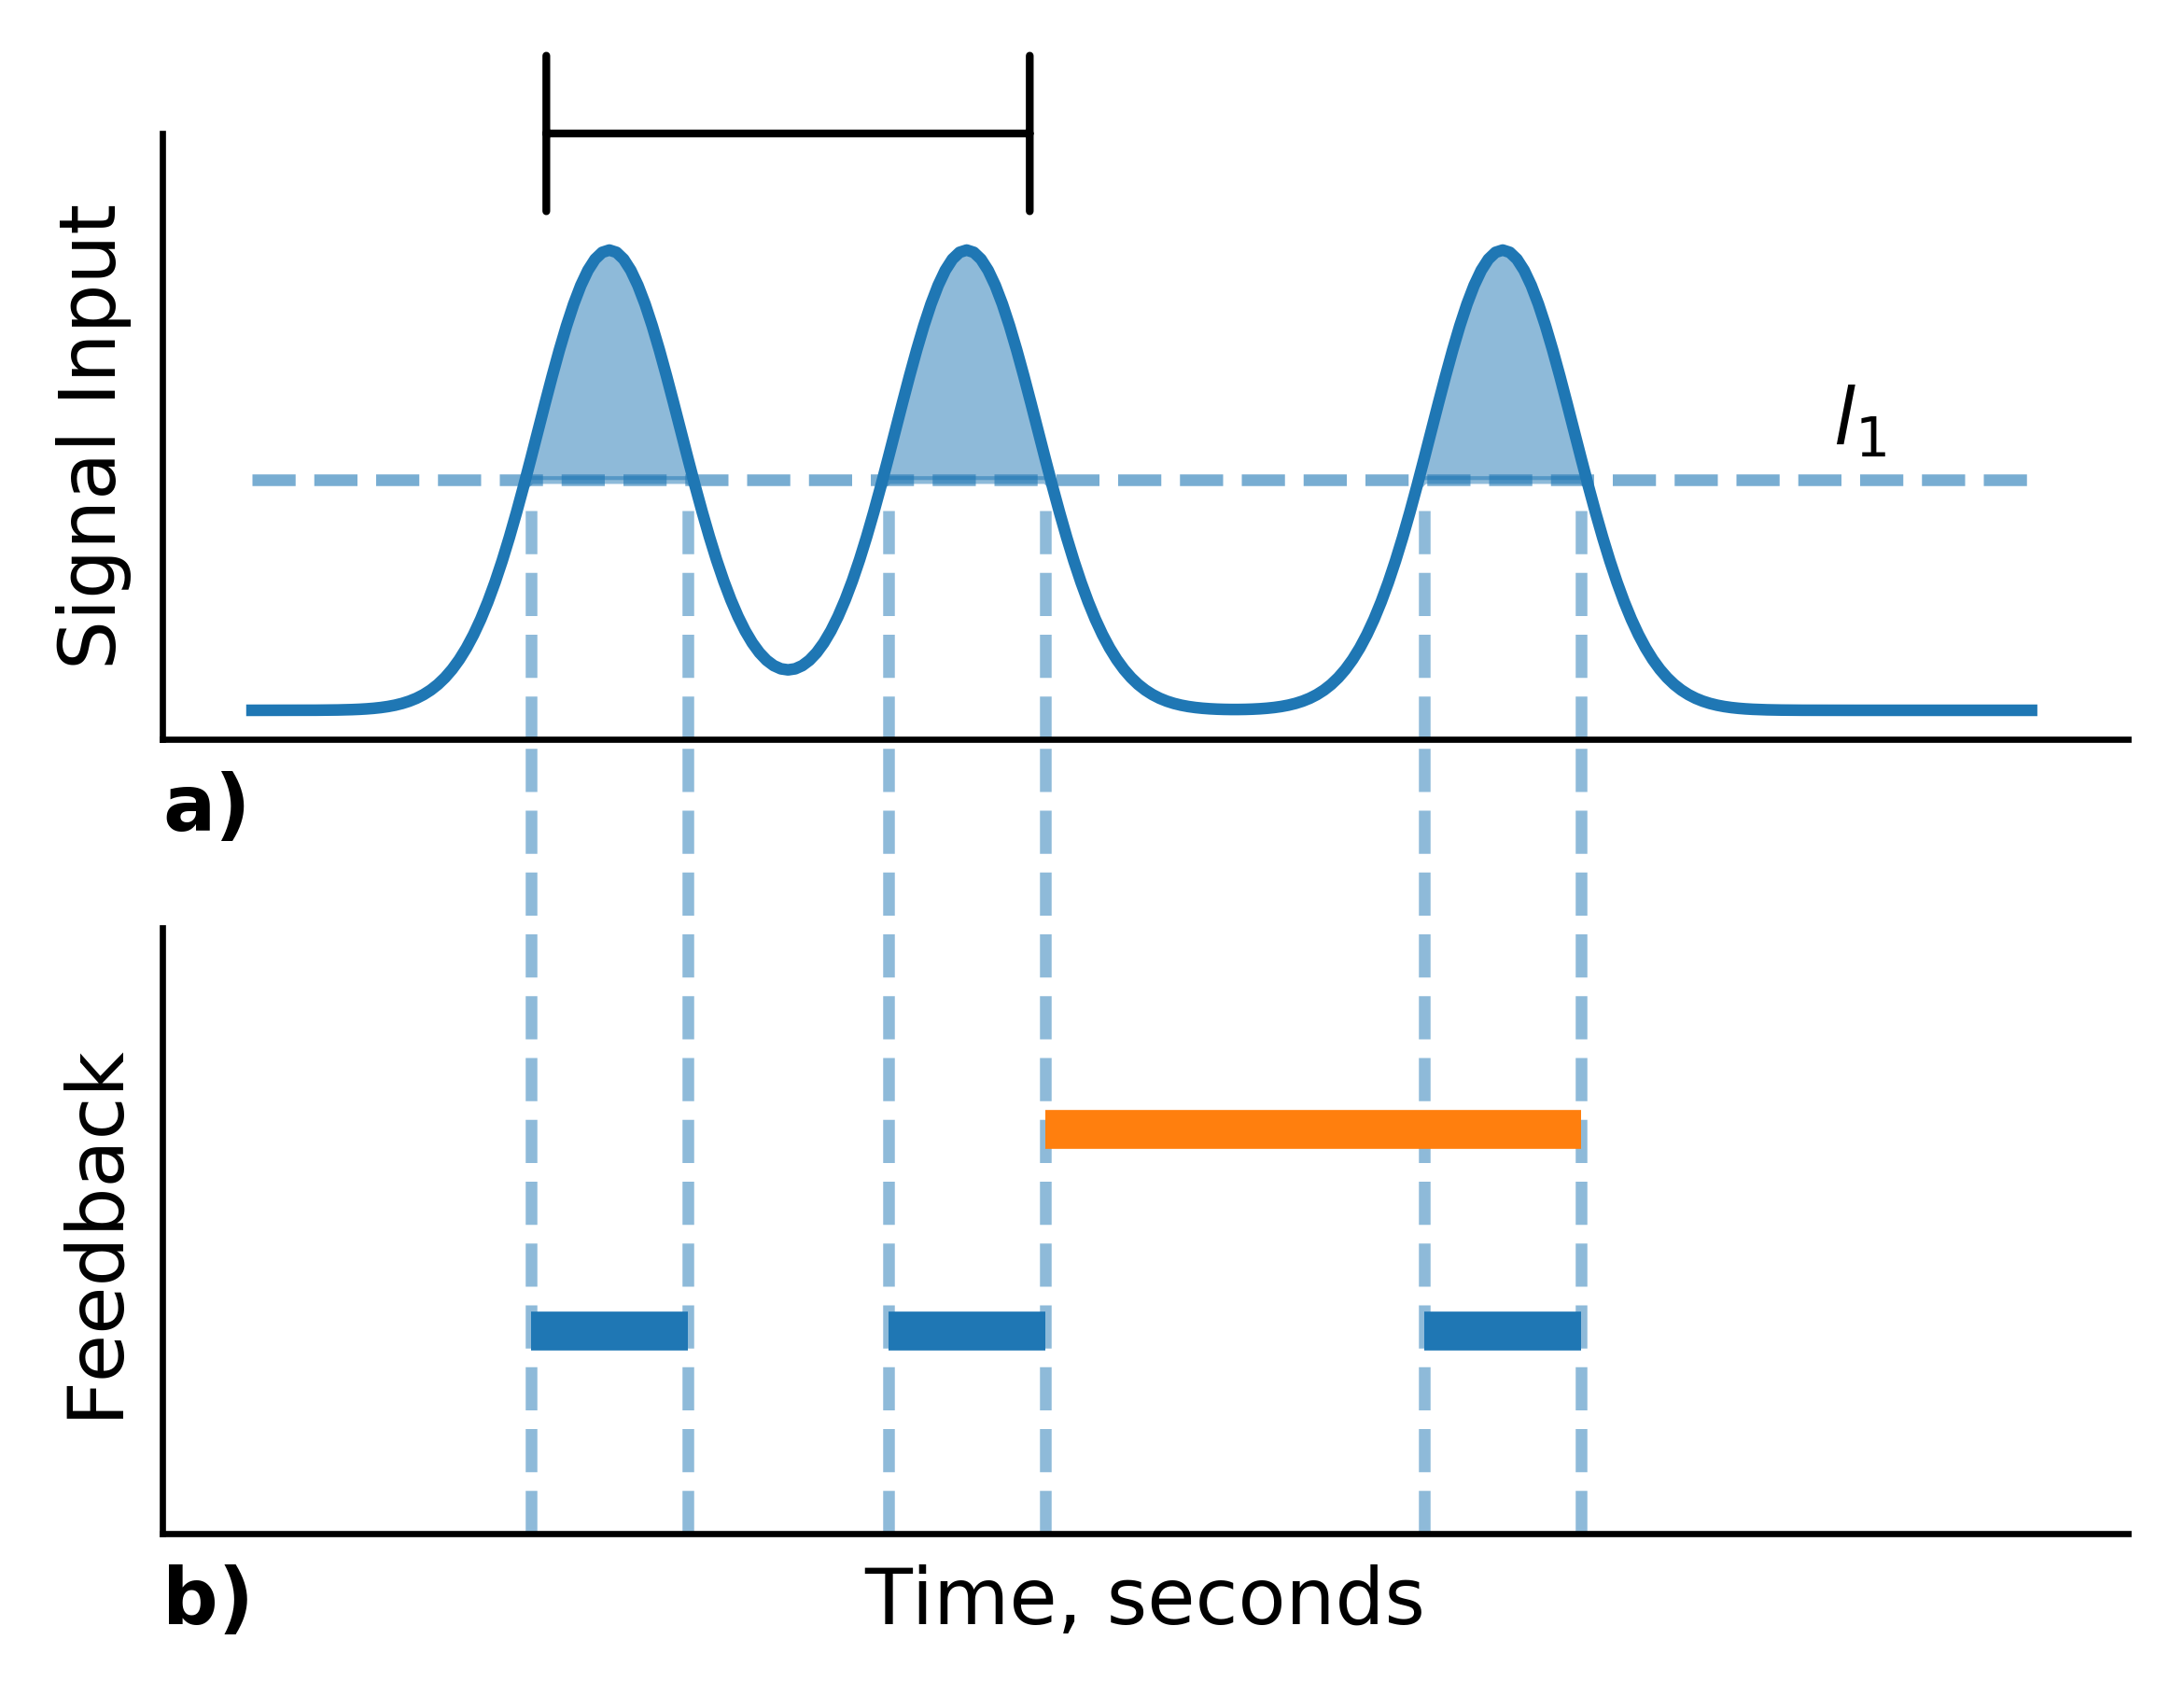
\includegraphics[height=.4\textwidth]{figures/EMG/Figure1}
	\caption[Illustrative signal input over time]{Illustrative signal input over time.
		a) The first two inputs select the command; the black bar represents the command time.
		The third input causes motion.
		The shaded areas indicate when the signal crosses the minimum threshold, $l_1$.
		b) Visual feedback is presented according to the bars (blue = Concurrent Feedback, orange = Terminal Feedback).}
	\label{figure:label1}
\end{figure}

Subjects completed 3 Code Accuracy Tests and 16 Blocks of testing during the experiment, see Figure~\ref{emg:experimentaldesign}.
The Code Accuracy Test was designed to evaluate subject's ability to enter commands, and each Test consisted of 20 randomly ordered commands (5 of each of the 4 commands).
The 16 Blocks were split into 12 Training Blocks, during which time the separate training methodologies were applied, and 4 Evaluation Blocks, during which time all subjects were exposed to same interface as the Control group.
Each Block consisted of 10 cursor-to-target trials, after which subjects completed the workload and trust surveys and had a 30 second break.

\begin{figure}[bt!]
	\centering
	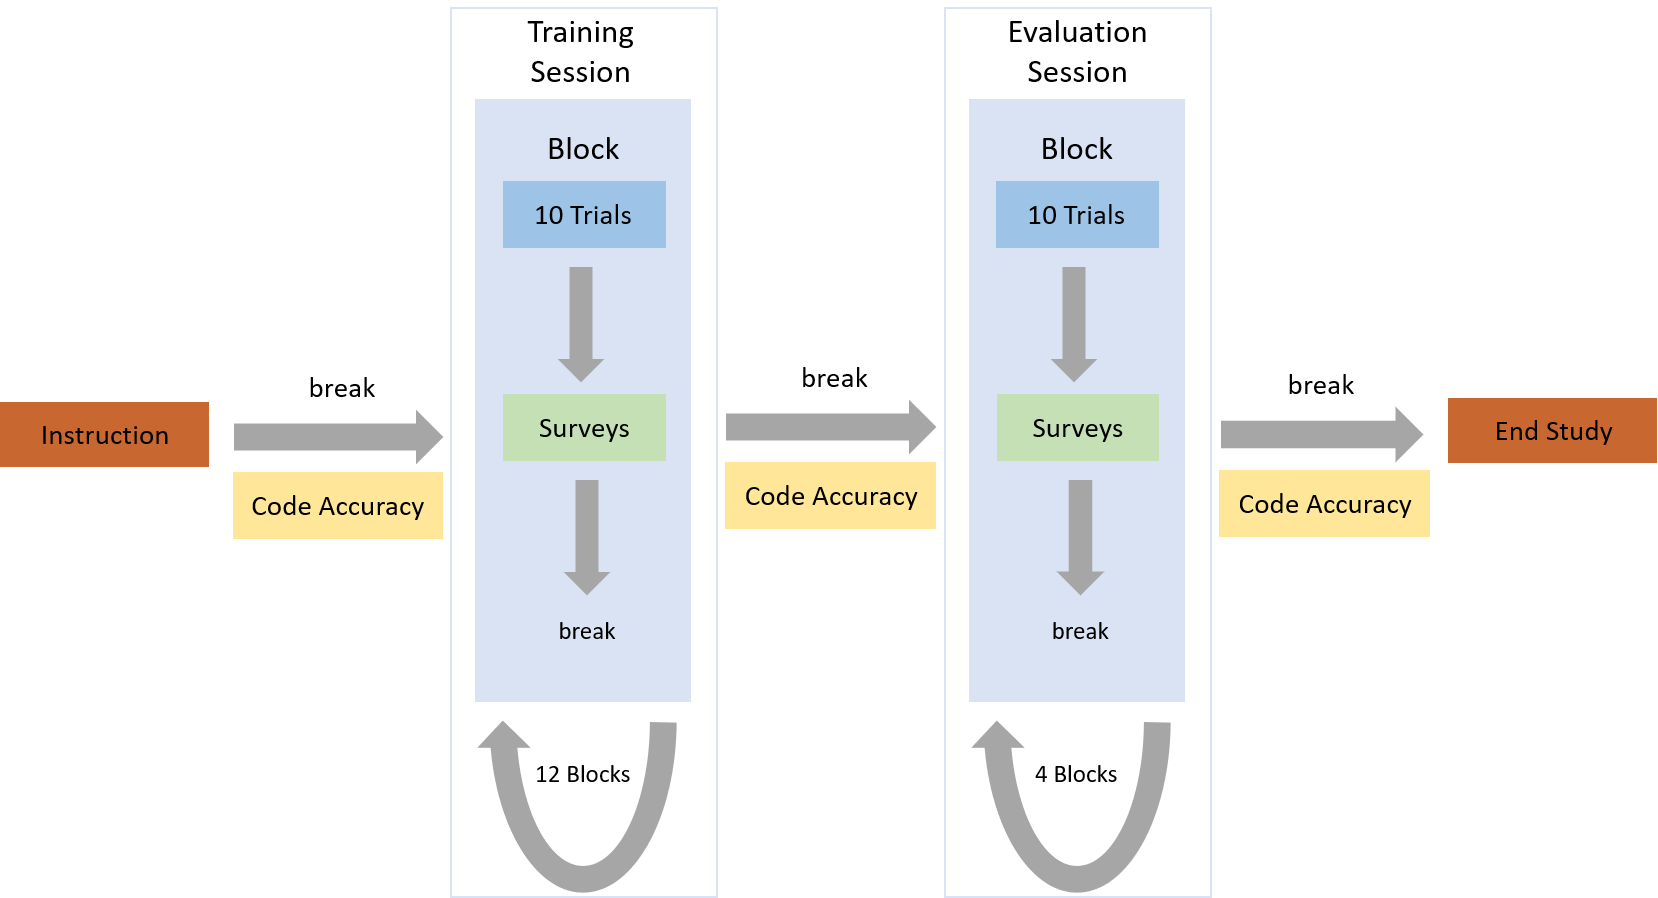
\includegraphics[width=\linewidth]{figures/EMG/Figure3}
	\caption[Experimental design flowchart]{Experimental design flowchart.}
	\label{emg:experimentaldesign}
\end{figure}

\section{Analysis and Hypotheses}
This experiment investigated the effect of training methodology on performance, workload, and trust.
The primary performance metric was the percentage of successful trials in a Block, and secondary metrics were the average trial time of successful trials and the throughput.
While a majority of the our metrics are analyzed by Block, trial time was analyzed by Session as the randomization of the 40 target positions occurred over 4 Blocks.
Trust and workload were each measured using surveys.
Trust was evaluated using \citeauthor{jian_foundations_2000}'s twelve statement questionnaire which measures trust between people and automated systems~\citep{jian_foundations_2000}.
Perceived workload was measured using Modified Bedford scale~\citep{roscoe_subjective_1990}.
These surveys were administered after each Block.
We also analyzed the results of the Command Accuracy Test, which was completed prior to training, after training, and after the retention phase at the end of the experiment.
During the Command Accuracy Test, subjects were asked to input each of the four commands 5 times, and the percentage of successful inputs was used as a metric of performance.

\subsection{Hypotheses}
Based on our prior experience with augmented feedback and sEMG cursor control, we formed the following hypotheses.

\begin{enumerate}
	\item During the training phase, the Concurrent Feedback group will have the highest performance followed by Terminal Feedback, then Control, and finally the Adaptive Threshold groups.
	\item All groups will perform similarly in the retention phase.
	\item The Concurrent Feedback and Terminal Feedback groups will have a high level of trust during training with some decrease during retention.
	      Although, the trust level will still remain high during retention.
	\item The Control group's trust will continually increase.
	\item The Adaptive Threshold group will have lower trust during training, which will increase in retention.
	\item The perceived workload will continually decrease during the training phase for all groups with the largest decreases for the Concurrent Feedback and Terminal Feedback groups.
	\item There will be no significant difference in workload in the retention phase for all groups.
\end{enumerate}

\section{Results}

We ran two-factor mixed models to investigate changes in performance, workload, and trust with one between-subjects factor, Group, and one within-subjects repeated measure, Block.
When significant effects were observed, post hoc comparisons using the Tukey Honest Significance Difference (HSD) test were performed and considered significant at the $p < 0.05$ level, and the Satterthwaite method was used to calculate the degrees of freedom.

\subsection{Performance Metrics}
The percent success metric measured the percentage of successfully completed Trials within a Block; a Block contained 10 Trials.
There were significant main factors of Group ($F(3, 44) = 8.18, p < 0.001$) and Block ($F(15, 660) = 31.80, p < 0.001$).
There was also a significant interaction effect between Group and Block ($F(45, 660) = 3.90, p < 0.001$).
Despite the presence of an interaction effect that resulted from subjects learning the task (as indicated by the Block factor), the main effect of Group could still be interpreted.
A Tukey test showed that the subjects in the groups differed significantly, with subjects in the Concurrent Feedback group performing significantly better than those in the Control group ($p = 0.020$).
The Tukey test also showed that subjects in the Adaptive Threshold group performed significantly worse than those in the Terminal Feedback and Concurrent Feedback groups ($p < 0.001, 0.01,$ respectively).

\begin{figure}[bt!]
	\centering
	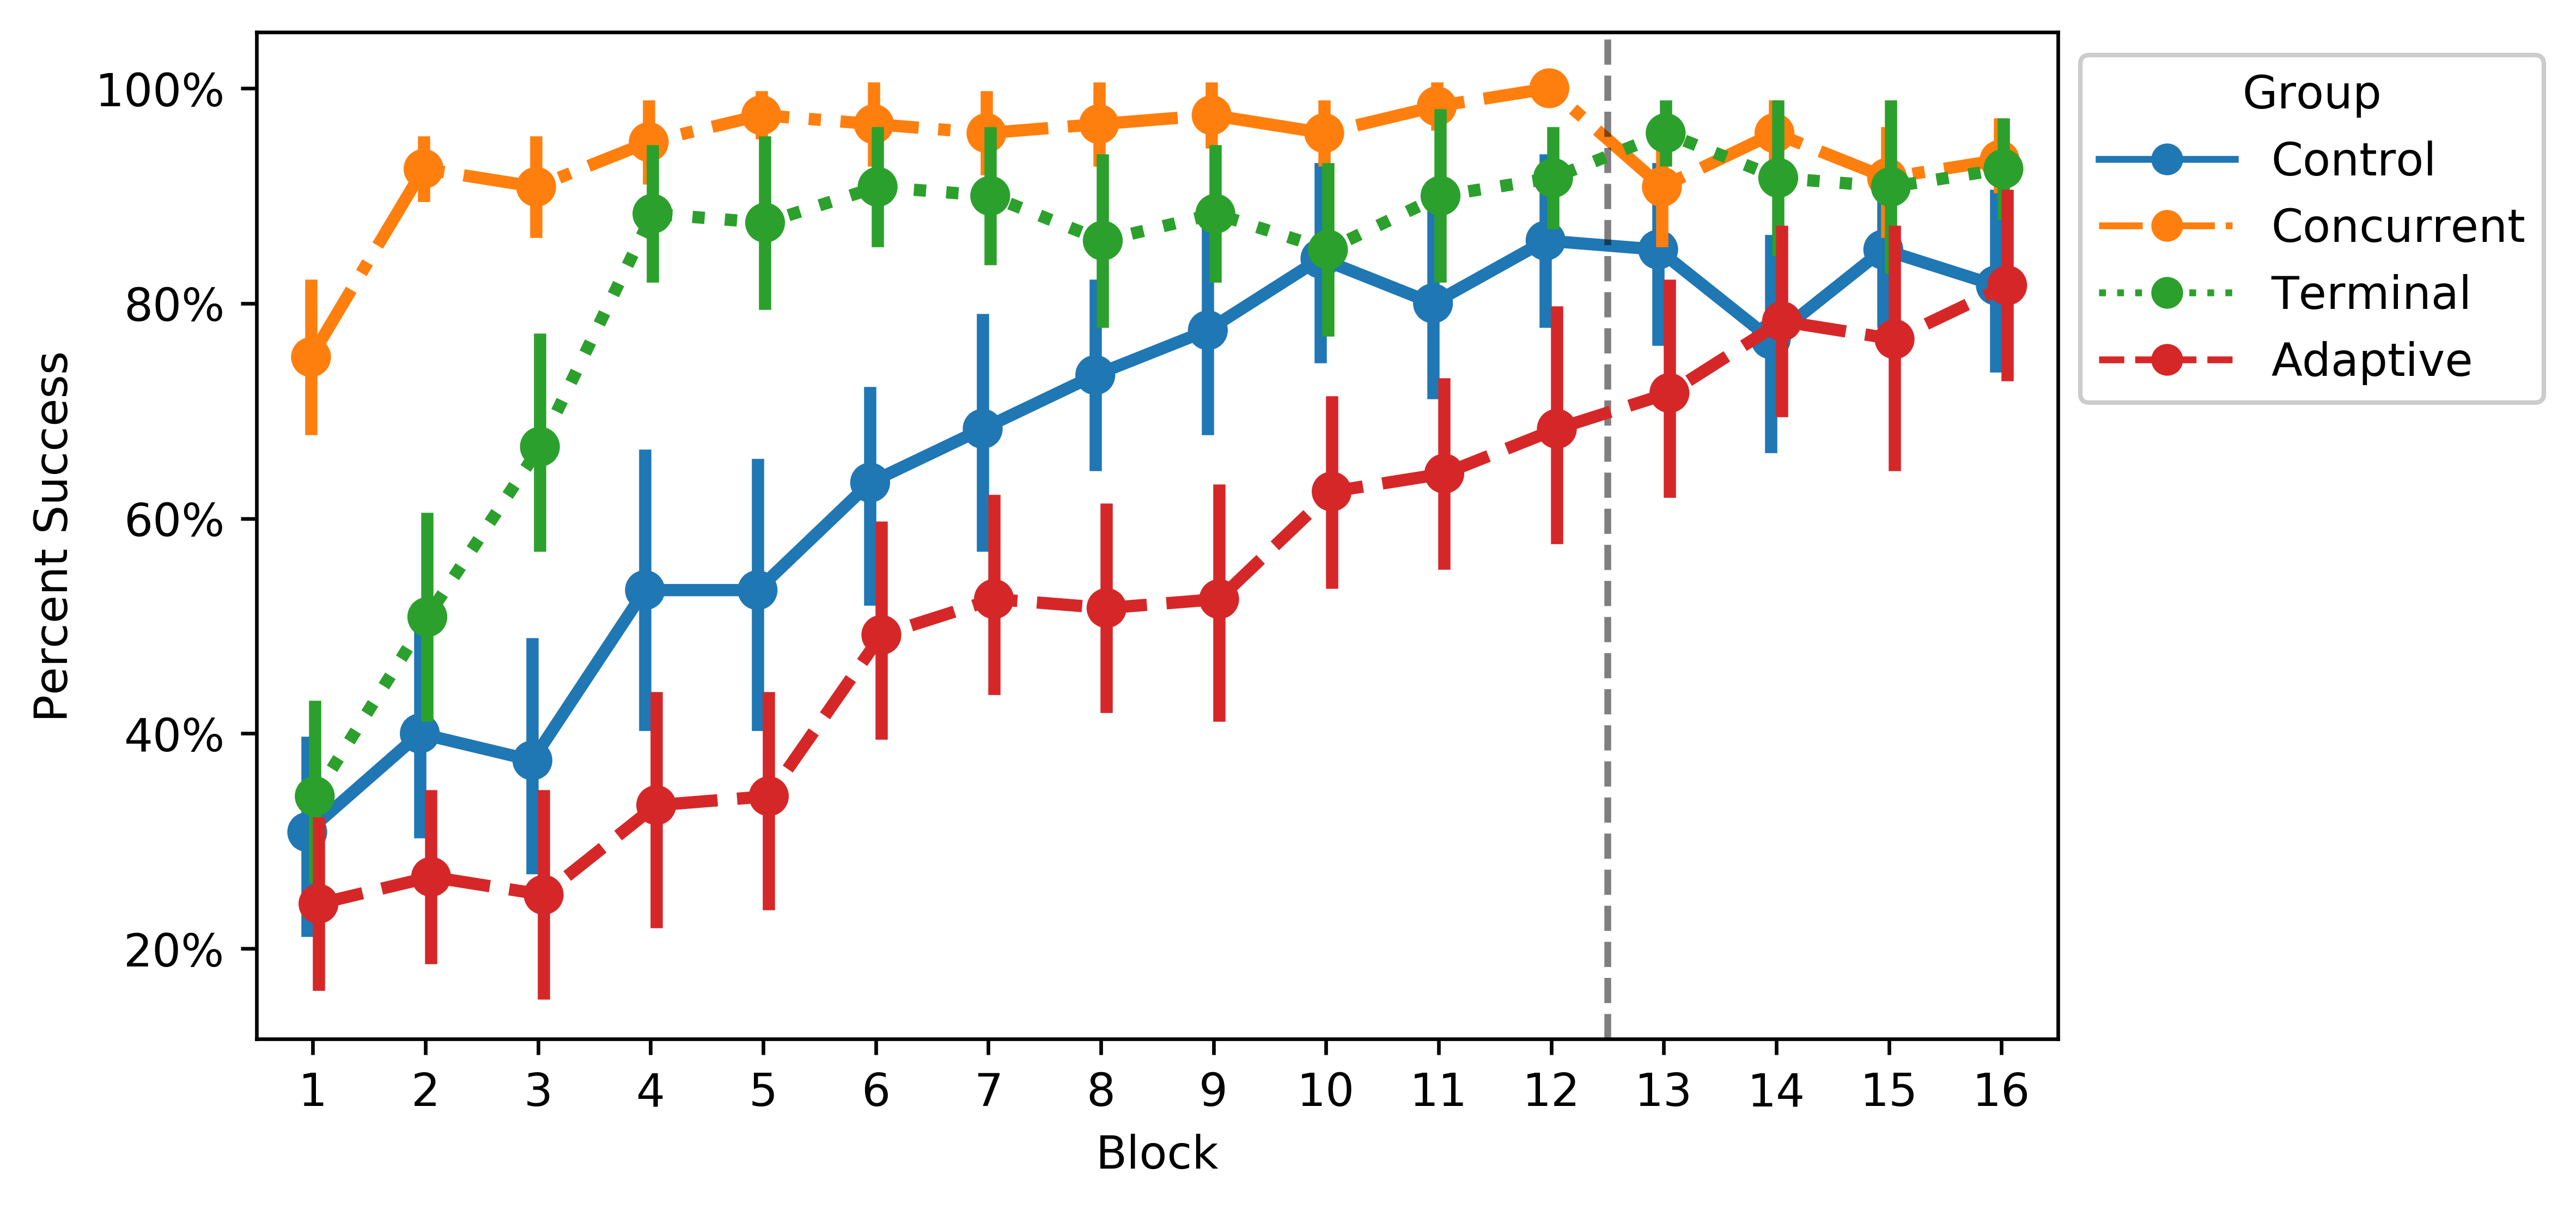
\includegraphics[height=.4\textwidth]{figures/EMG/PercentSuccess}
	\caption[Percent success by Block across groups]{Percent success by Block across groups.
		The vertical dashed line represents the transition from the training phase to the retention one.
		Error bars shown are the standard error of the mean.}
	\label{figure:label3}
\end{figure}

The interaction effect resulted from different learning rates between the groups (see Figure~\ref{figure:label3}), where subjects learned in the following order (fastest to slowest): Concurrent Feedback, Terminal, Control, and Adaptive Threshold.
Compared to the Control group, the Concurrent Feedback group significantly outperformed them for the first 6 Blocks.
Unlike the Concurrent Feedback group, the Terminal Feedback and Adaptive Threshold groups started with the same initial performance as the Control group.
The Terminal Feedback group learned more quickly than the Control group, however, and significantly outperformed the Control group for Blocks 4 and 5.
Compared to the Control group, all groups performed at statistically similar level after Block 6.
Investigating the immediate retention effects when the group-specific treatments are removed in Block 13, the mixed model showed no change in performance for any of the groups ($p > 0.99$ for all groups).
As such, the percentage of successfully completed Trials did not show any effect from the guidance hypothesis (i.e. the subjects did not rely on the feedback to complete the task and removing the feedback did not result in decreased performance).

The throughput was calculated for the retention phase and averaged across Blocks 13 through 16 (i.e. Session 4).
Throughput is generally used to assess an input device, which should be measured when the subjects can complete the task.
Since there were no significant differences in the retention phase for percent complete, it was logical to only calculate throughput at this time.
There was no significant difference in throughput between the Groups ($F(3, 44) = 1.62, p < 0.20$).
The mean throughput for all subjects was found to be 0.56 $\pm$ 0.02 bits/s ($\mu\pm\sigma$).

The randomization of the 40 target positions occurred over 4 Blocks, thus it seemed appropriate to average Trial time over a Session (i.e. set of 4 Blocks).
Trial time was only defined for successfully completed Trials, and the Satterthwaite method was used to calculate the adjusted degrees of freedom using the lmerTest package in R~\citep{RN53}.
The results are displayed in Figure~\ref{figure:label4}.
There were significant main factors of Group ($F(3, 43.97) = 4.39, p < 0.01$) and Session ($F(3, 131.07) = 24.91, p < 0.001$).
The interaction effect between Group and Session was not significant ($F(9, 131.07) = 0.78, p = 0.63$).
A Tukey test showed that the Concurrent Feedback group performed significantly better than those in the Adaptive Threshold group ($p = 0.004$), which was the only significant difference between groups.
No groups significantly outperformed the Control group.
Analysis of the Session factor showed increased performance ($p < 0.05$) until the last two Sessions, which were not statistically different ($p = 0.65$).
These results further supported that the guidance hypothesis did not occur.

\begin{figure}[bt!]
	\centering
	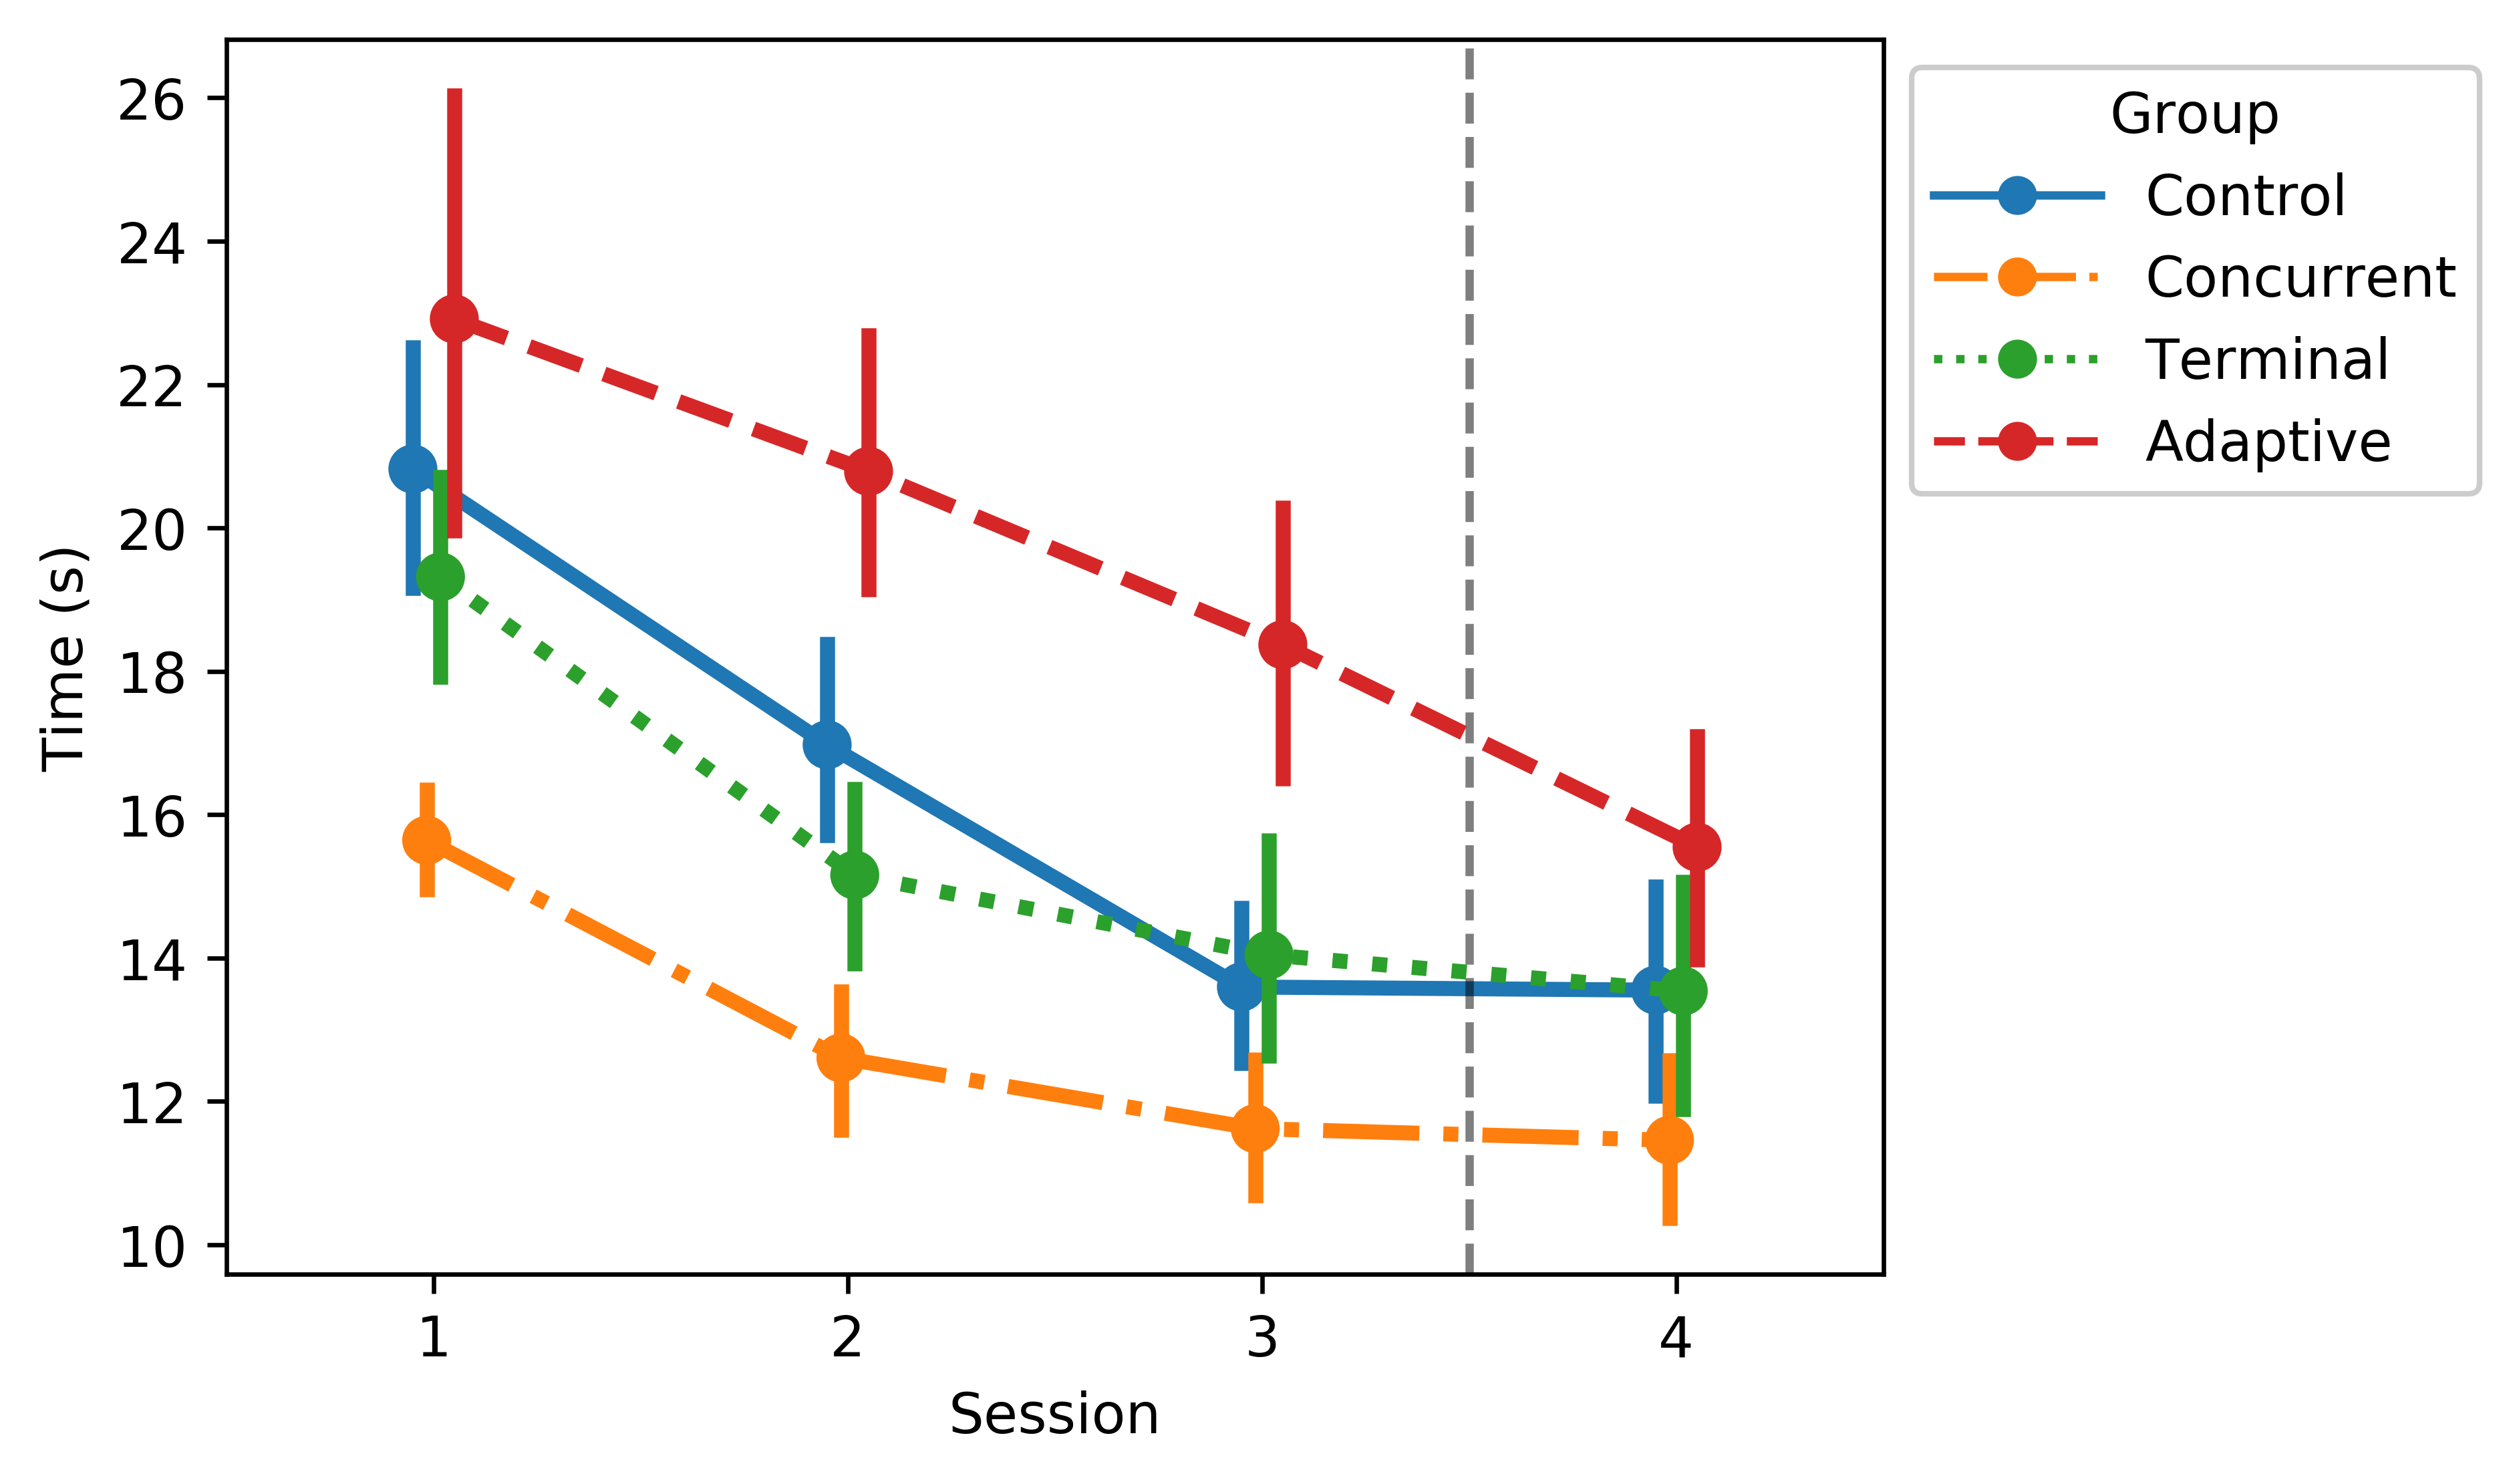
\includegraphics[height=.4\textwidth]{figures/EMG/TrialTime_session}
	\caption[Average Trial time by Session across groups]{Average Trial time by Session (sets of 4 Blocks) across groups.
		The vertical dashed line represents the transition between the training and evaluation phases.}
	\label{figure:label4}
\end{figure}

\subsection{Trust and Perceived Workload}
The Modified Bedford Workload metric is a subjective measurement of perceived workload that ranges from 1-10, where 1 indicates low workload and 10 indicates high workload.
There was a significant main factor of Block ($F(15, 660) = 18.29, p < 0.001$), but Group was not found to be significant ($F(3, 44) = 2.16, p = 0.106$).
There was also a significant interaction effect between Group and Block ($F(45, 660)= 1.82, p = 0.001$) (see Figure~\ref{figure:label5}).
The interaction effect resulted from subjects reporting lower workload as they learn the task at different rates, as indicated by the Block factor.
In further investigation of the interaction, we observed that the Adaptive Threshold group reported a significantly higher workload than the Concurrent Feedback group for Blocks 9, 10, and 11.
This perception of high workload may possibly have resulted from the significantly worse performance of the Adaptive Threshold group.
None of the groups showed a significant difference in workload compared to the Control group and all four groups reported statistically similar workloads in the retention phase.

\begin{figure}[bt!]
	\centering
	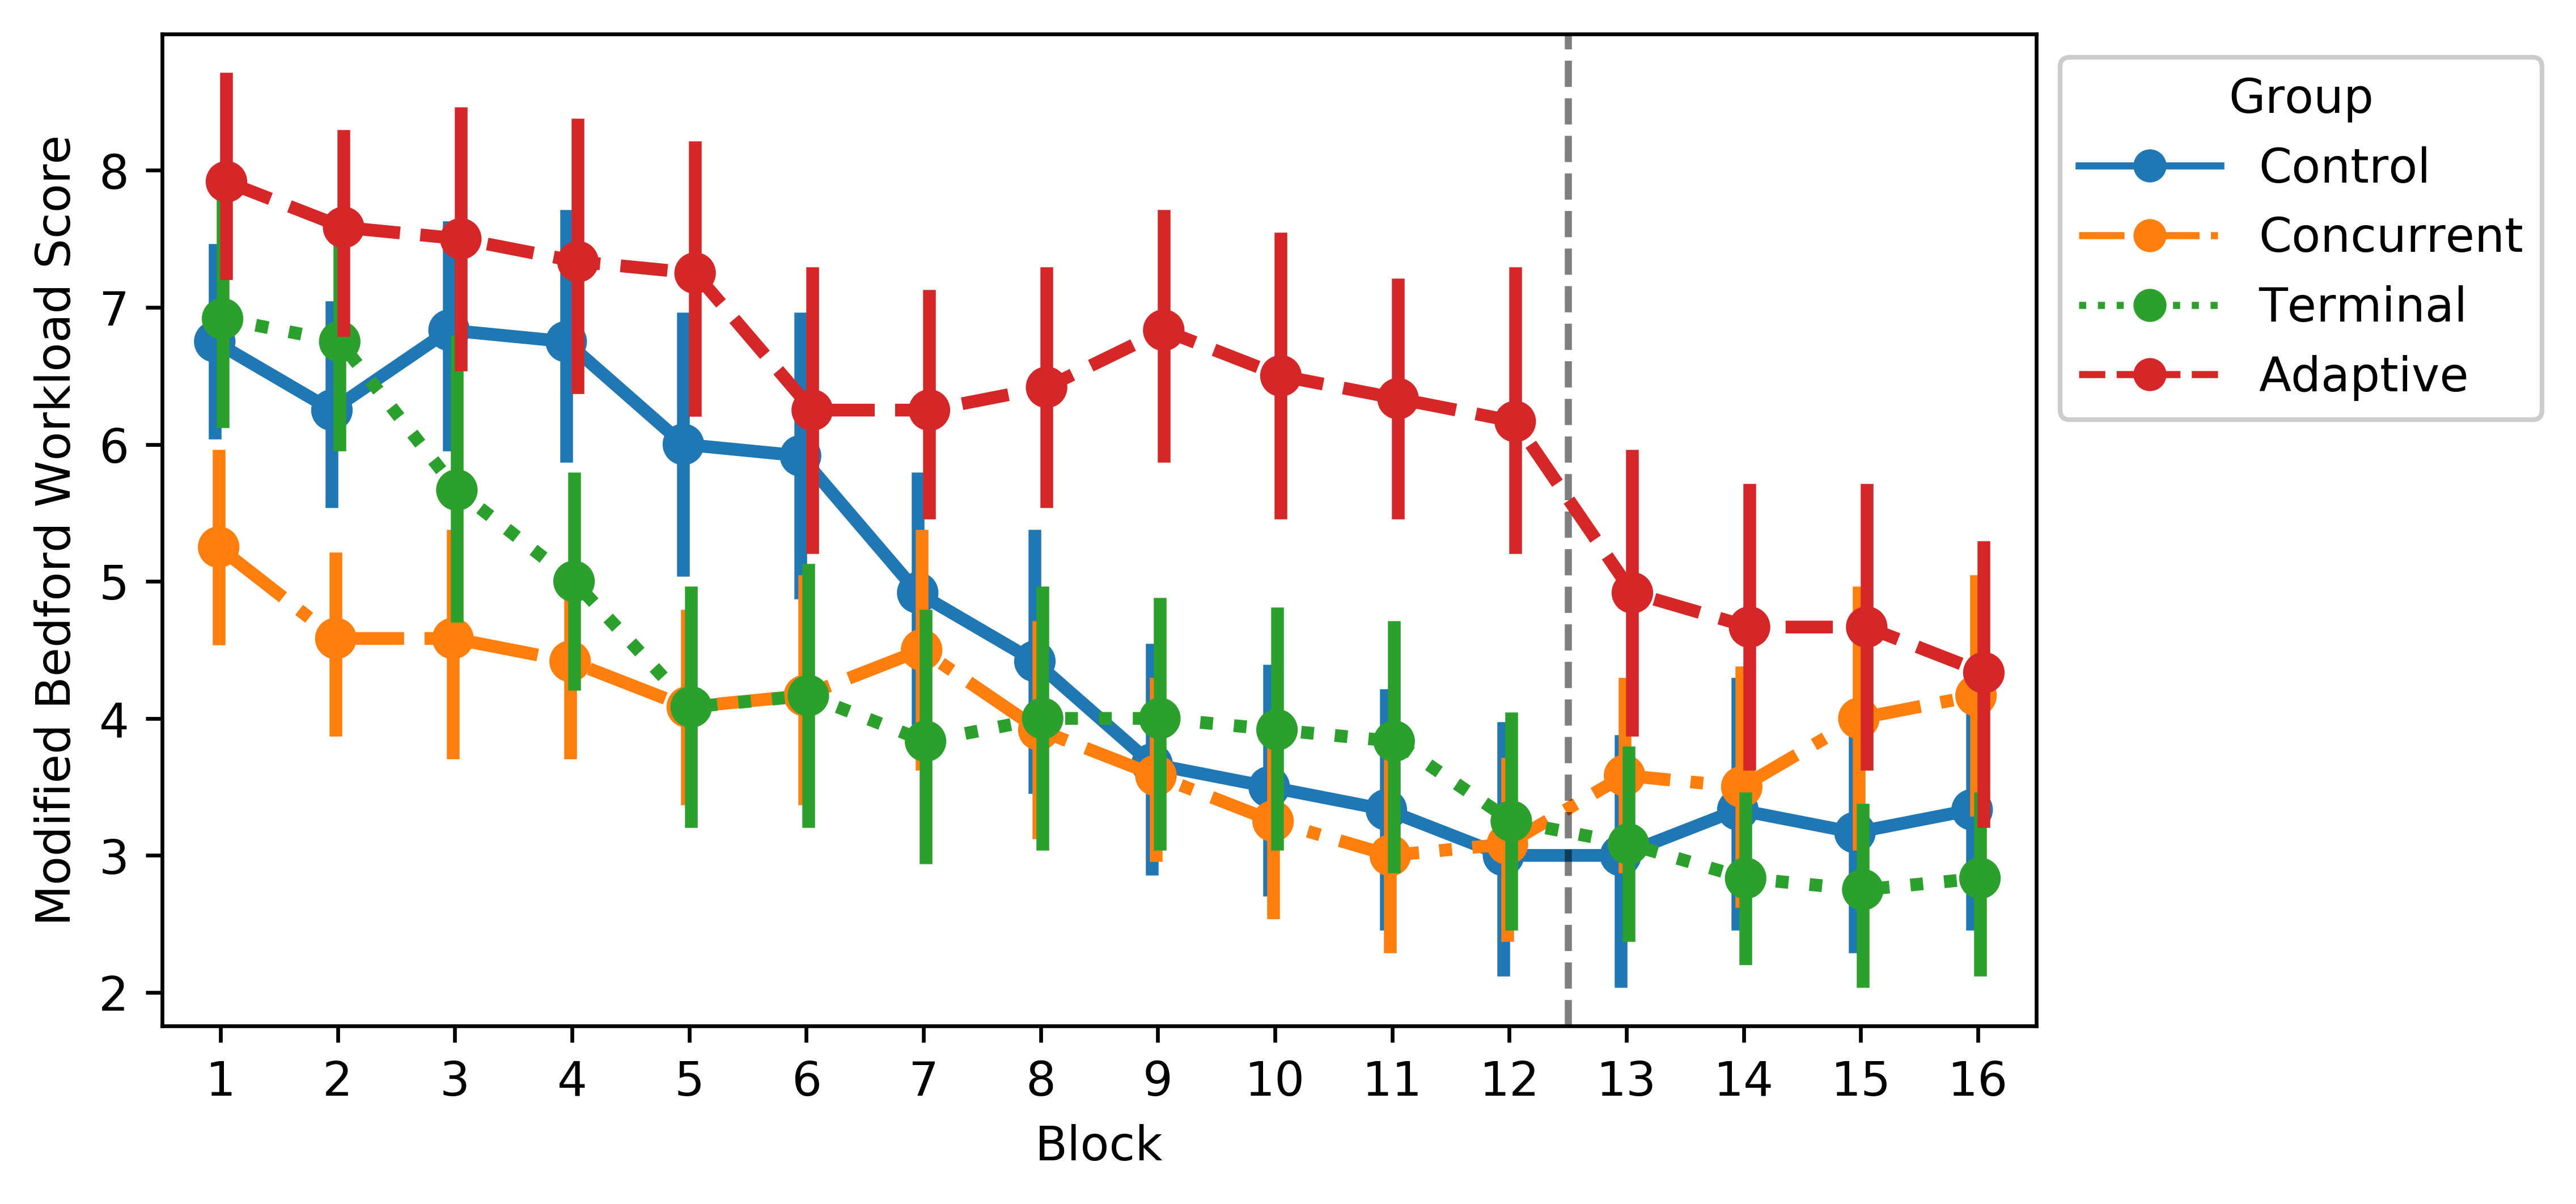
\includegraphics[height=.4\textwidth]{figures/EMG/ModifiedBedfordWorkloadScore}
	\caption[Modified Bedford Workload Score by Block across groups]{Modified Bedford Workload Score by Block across groups.
		The vertical dashed line represents the transition from the training phase to the retention one.
		Error bars shown are the standard error of the mean.}
	\label{figure:label5}
\end{figure}

Intragroup changes in workload were also of interest.
The Concurrent Feedback group showed no statistically significant changes in performance between Blocks, though they did demonstrate a nonsignificant, increasing workload trend in the retention phase of the experiment.
The Terminal Feedback group had statistically higher initial workload for Blocks 1, 2, and 3, but the remainder of the Blocks had a statistically similar level of workload.
The Control group's workload was significantly higher for Blocks 1-6, possibly due to their slower learning rate, but leveled off for the remainder of the Trials.
Finally, the Adaptive Threshold group reported the highest workload in Blocks 1-5, but also saw the largest improvement transitioning into the retention phase where their $l_1$ threshold stabilized to the same fixed value as the other groups.

Trust was measured using Jian's twelve question trust survey~\citep{jian_foundations_2000}.
Each question was rated on a 7-point Likert scale, the five reverse coded questions were reversed, and the results were averaged to create a single trust score (see Figure~\ref{figure:label6}).
There was a significant main factor of Block ($F(15, 660) = 13.05, p < 0.001$), but Group was not found to be significant ($F(3, 44) = 2.59, p = 0.065$).
There was also significant interaction effect between Group and Block ($F(45, 660) = 2.00, p < 0.001$).
The significant main effect of Block showed a gradual increase in trust throughout the duration of the study.
After investigating the interaction effect, we saw that no group reported a significantly different trust level than the control group on any Block, but that the Adaptive Threshold group recorded a significantly lower trust than the Concurrent Feedback group on Blocks 3-6 and 9.
Similar to workload, the primary interaction effects appeared driven by intragroup differences.
The Concurrent Feedback group showed no statistically significant changes through the study, the Terminal Feedback and Control groups displayed significant increases in trust in Blocks 1-6, and the Adaptive Threshold group reported significantly higher trust in the retention Session than during early Blocks.

\begin{figure}[bt!]
	\centering
	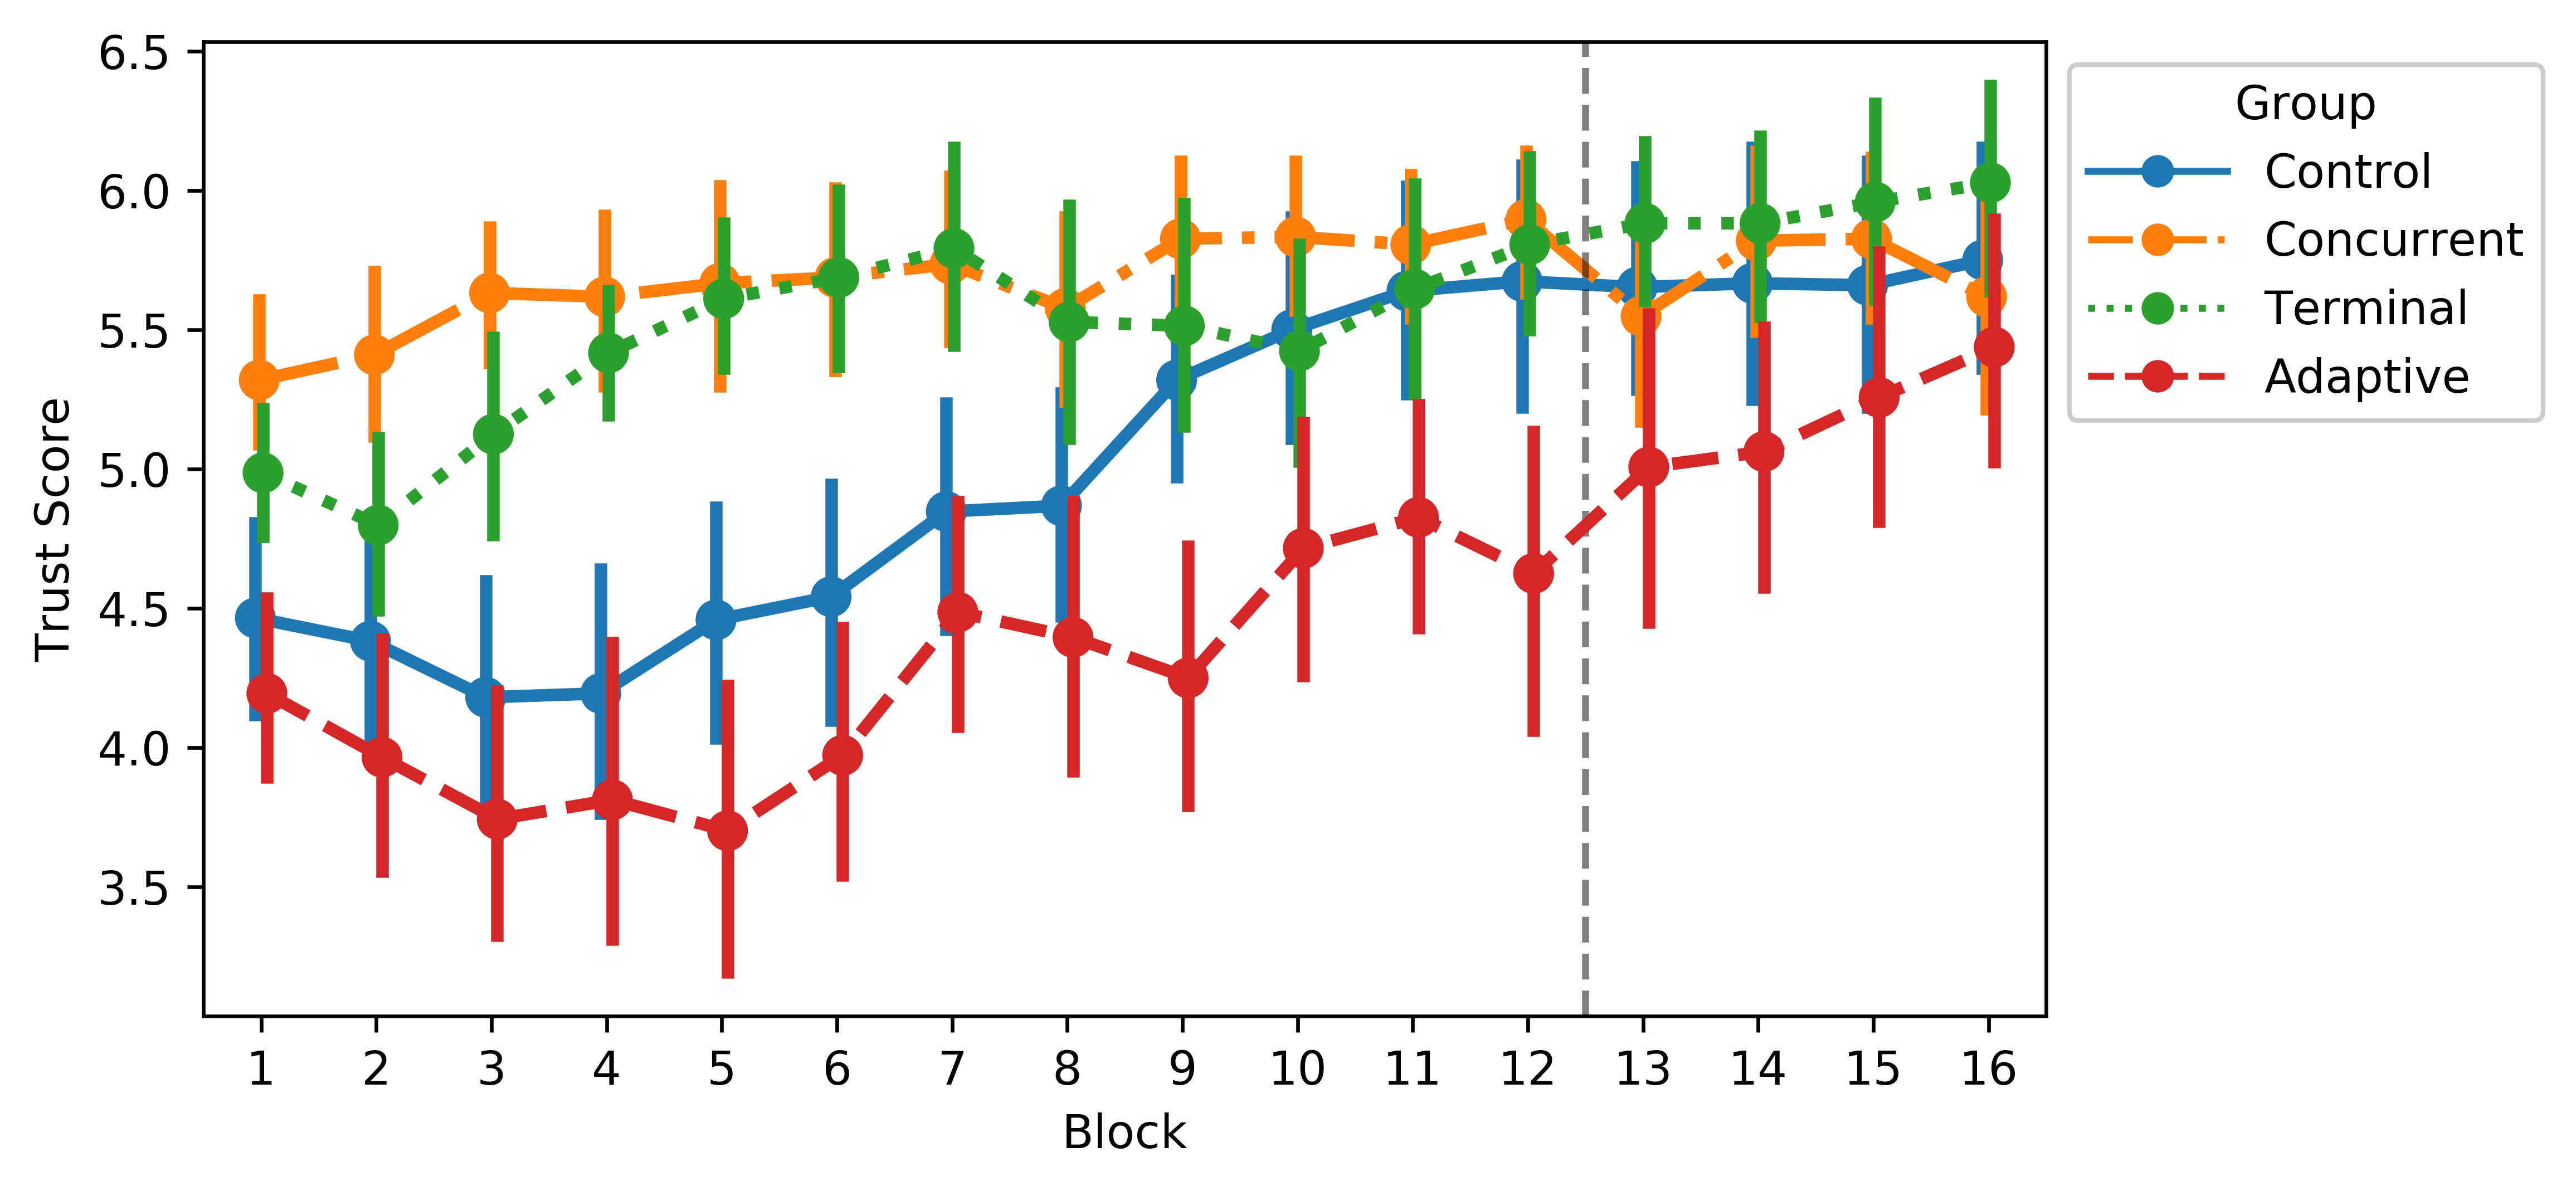
\includegraphics[height=.4\textwidth]{figures/EMG/TrustScore}
	\caption[Trust Score by Block across groups]{Trust Score by Block across groups.
		The vertical dashed line represents the transition from the training phase to the retention one.
		Error bars shown are the standard error of the mean.}
	\label{figure:label6}
\end{figure}

\subsection{Command Accuracy}
In contrast to previous results, the results in this section are not reported by Block or Session.
The Command Accuracy Test occurred three times (before Block 1, after Block 12, and after Block 16), and the average was calculated for each Test.

In each Command Accuracy Test, subjects responded to prompts to perform commands.
The command accuracy percent indicates the percentage of the 20 prompts in each Test that subjects correctly performed.
Results were averaged by group (see Figure~\ref{figure:label7}).
There was a significant main factor of Test ($F(2, 88) = 108.48, p < 0.001$), but Group was not significant ($F(3, 44) = 2.63, p = 0.06$).
The interaction effect between Group and Test was not significant ($F(6, 88) = 0.82, p = 0.55$).
Investigation into the Test variable showed that subjects performed significantly better between Test 1 and 2, and between Test 1 and 3, but not between Test 2 and 3.
These results demonstrated that there was a significant improvement in the percent of commands accurately entered after the training portion of the experiment was finished.

\begin{figure}[bt!]
	\centering
	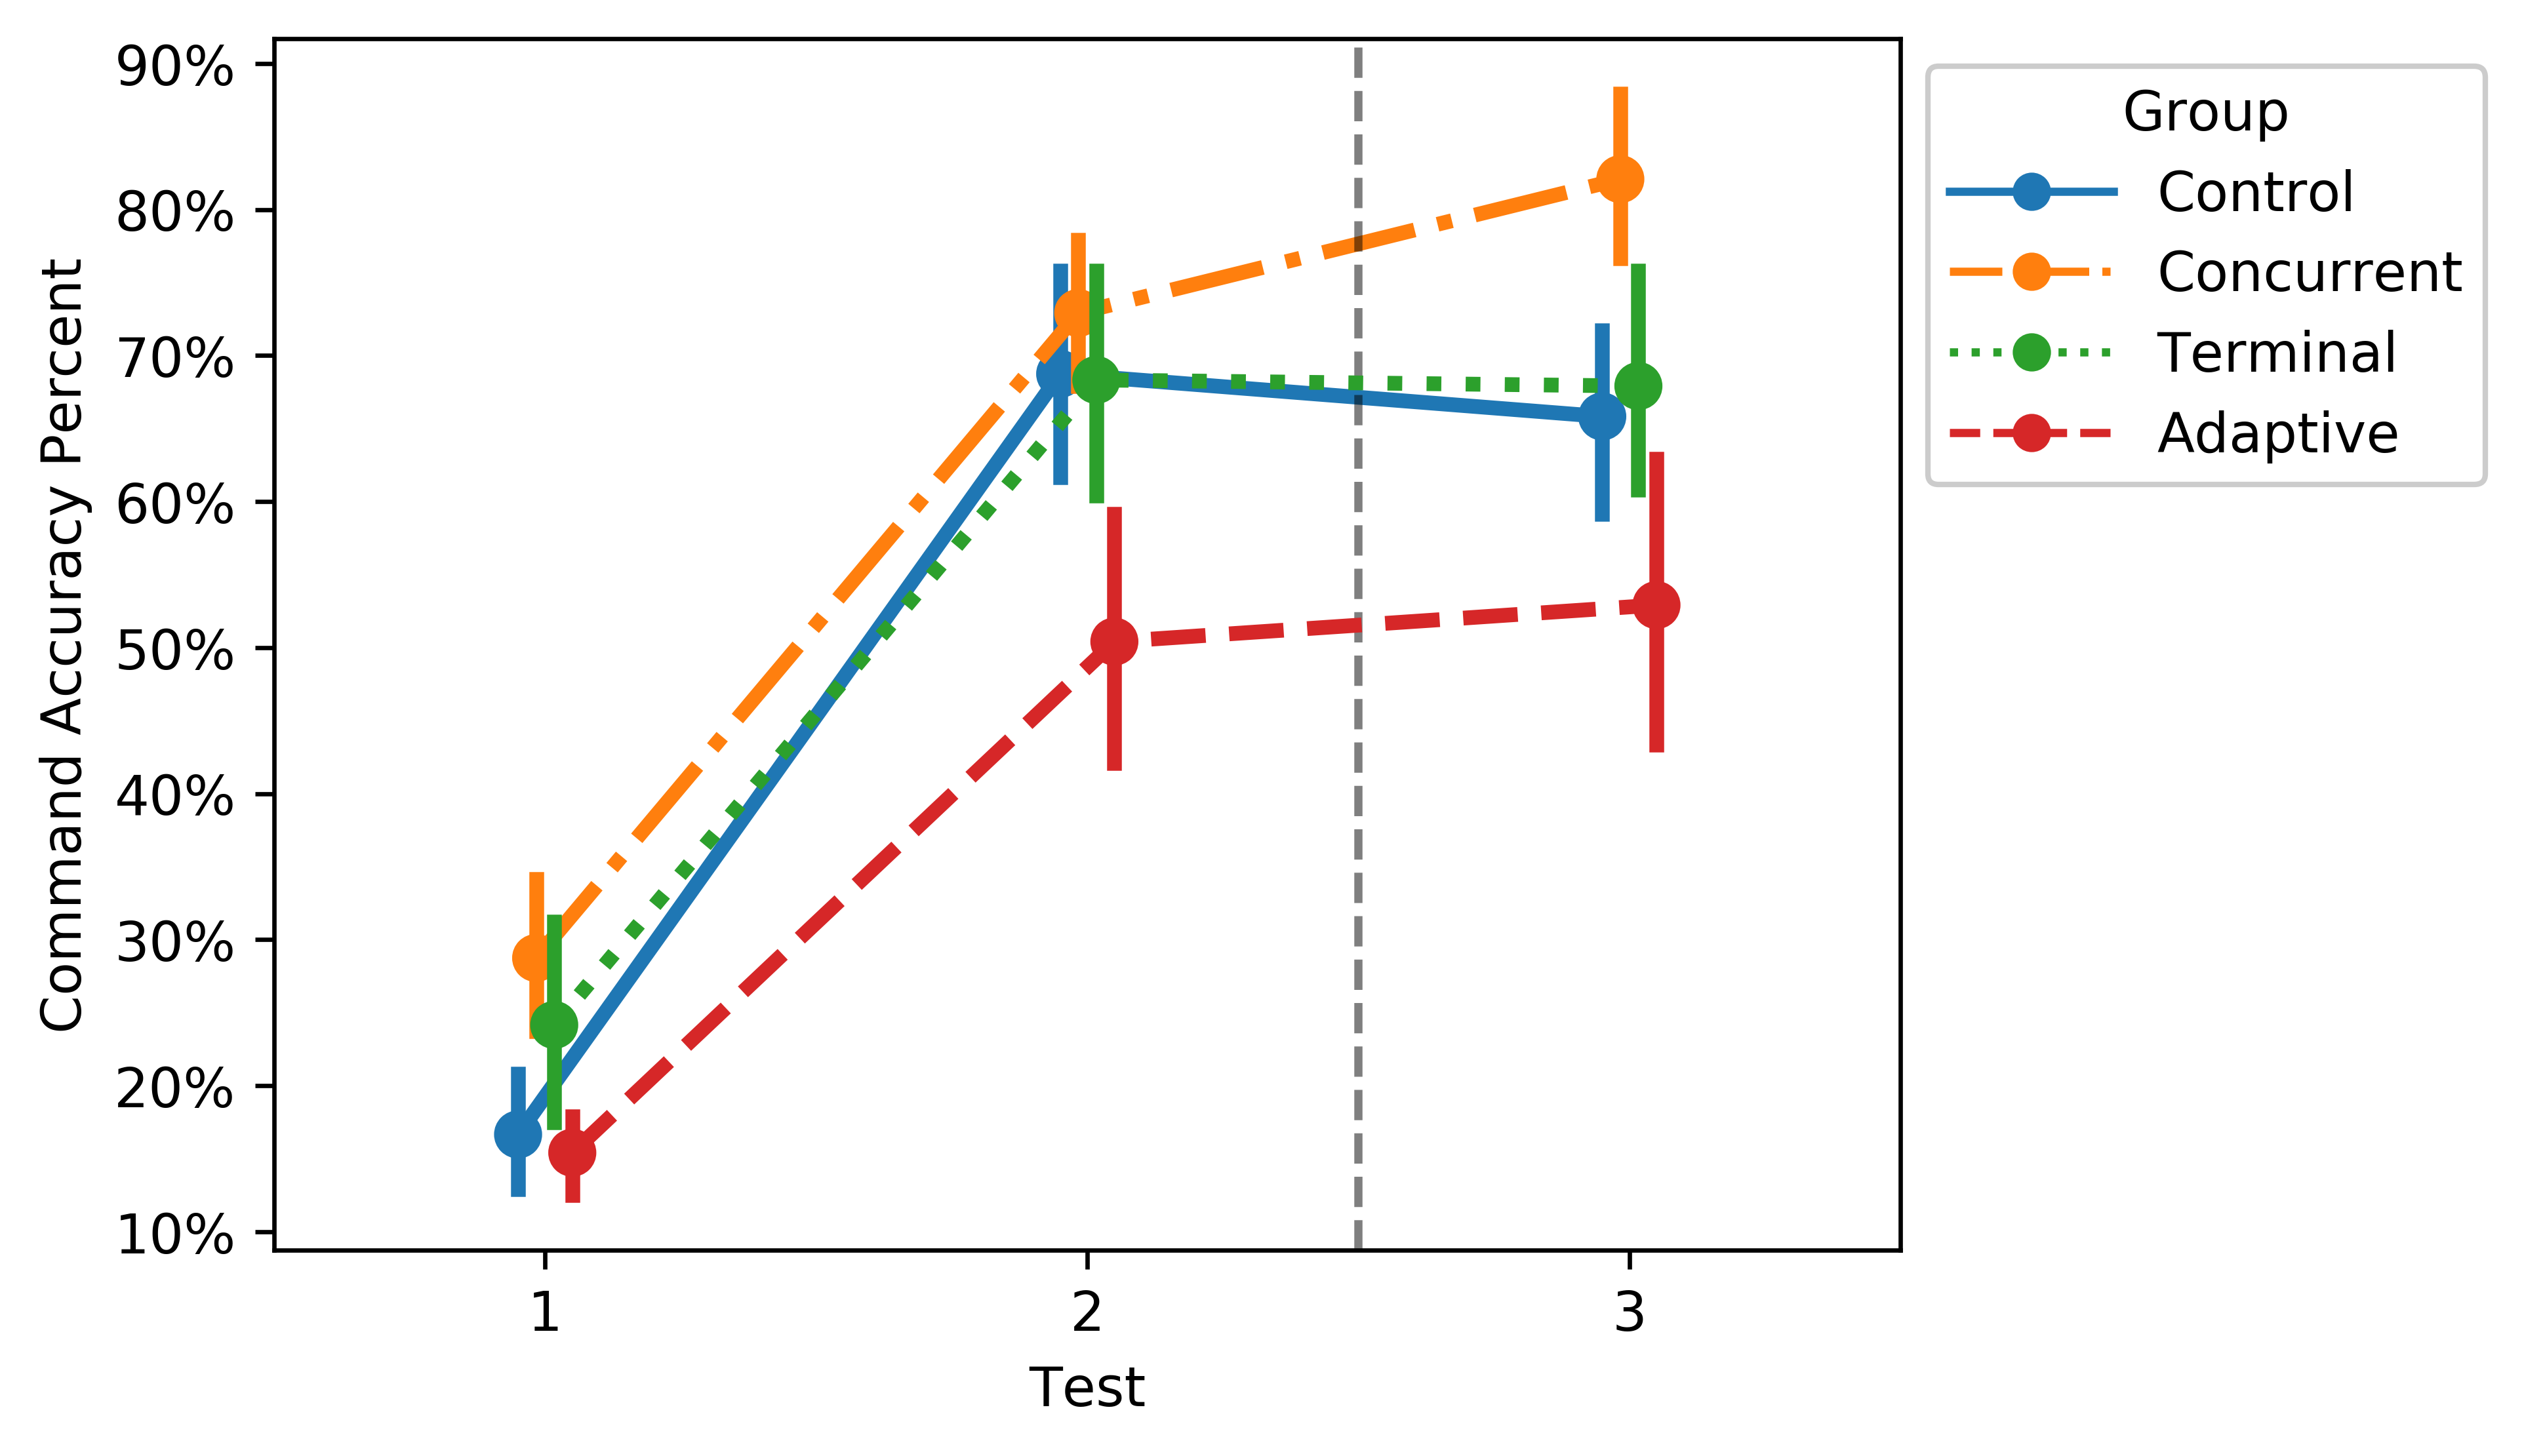
\includegraphics[height=.4\textwidth]{figures/EMG/CodeAccuracySuccess_session}
	\caption[Command Accuracy results by Test across groups]{Command Accuracy results by Test across groups.
		Test 1, 2, and 3 occurred prior to the training phase, after the training phase, and after the retention phase, respectively.}
	\label{figure:label7}
\end{figure}

\section{Discussion}
The study results elucidated a relationship between performance, workload, and trust that was influenced by the training methodology.
The Concurrent Feedback group started with the highest performance, lowest workload, and highest level of trust.
By the 5th Block, the Terminal Feedback group overlapped with the Concurrent Feedback group in terms of percent success, workload, and trust.
These two groups then tracked each other for the remainder of the study.
The Concurrent Feedback and Terminal Feedback groups did not have significantly different average trial times throughout the study.
The initial learning of these two groups differed with the Concurrent Feedback group demonstrating high performance with smaller, incremental gains and the Terminal Feedback group with larger Block-to-Block improvements.
The Control and Adaptive Threshold groups did not appear to reach a performance plateau for the percent success and steadily improved in subsequent Blocks.
Interestingly, the trust score also continually increased for both the Control and Adaptive Threshold groups.
Although the changing cursor dynamics in the Adaptive Threshold group does not seem to adversely affected trust compared to the Control group, the Adaptive Threshold group did report a significantly higher perceived workload for Blocks 9-12---the last four Blocks in the training phase.
Once the cursor dynamics stabilized, the perceived workload in the Adaptive Threshold group was not statistically different from the other groups.
These results suggested that visual feedback led to earlier performance gains with improvements in trust and workload.
The adaptive training methodology surprisingly did not adversely affect trust, but the cost was reflected in the performance and perceived workload.
Overall, all training methodologies achieved statistically similar results during the retention phase.

Measuring performance by percent success assessed the ability to complete the cursor-to-target task in the allotted 60 s.
The average trial time provided more insight into the group's performance.
The trends in the average trial time may be explained by the Command Accuracy Test results.
Higher percentages of command accuracy tracked with lower average trial times.
This relationship was expected as less time was spent attempting to input the command when the subject was able to accurately convey the inputs.
Although there were no statistically significant differences between groups in the retention phase for these metrics, it was notable that the Adaptive Threshold group consistently performed worse than the Concurrent Feedback group.

The Adaptive Threshold group did not outperform any group in any metric during the retention phase.
The results from this group were interesting for two reasons.
Firstly, an adaptive training methodology did not appear to cause adverse effects compared to the Control group.
Unreliable automation behavior can lead to poor human-automation interaction~\citep{RN54}, but was not the case in this study.
Secondly, the benefits of increased adaption induced by uncertainty did not manifest (e.g. generalization for novel tasks).
The adaption training methodology may be better tested with a different task with the same underlying structure instead of returning to a stable condition.
For example, \citeauthor{RN36} showed that subjects trained with an adaptive training strategy were able to quickly generalize to novel tasks with similar underlying structure.
It is also possible that the cursor dynamics unpredictability was not sufficiently large compared to the inherent sEMG control noise.

Our results aligned with previously published research.
The Concurrent Feedback and Terminal Feedback groups follow the findings of \citeauthor{RN27} that augmented feedback can improve performance.
We also observed effects that may be explained by \citeauthor{RN39}'s three layer model.
At times, there were significantly different levels of trust between the groups, which indicated that the training methodologies altered situational trust.
Subjects' trust levels also increased, which supported the notion of learned trust.
While developing a brain computer interface (BCI) was not the study objective, the throughput values during the retention phase for all groups fell within published results for sEMG cursor control systems.
Our previous single-site sEMG cursor control system with 2 DOF (counterclockwise rotation and forward) reported 2.24 bits/s and 0.23 bits/s for control methodologies that used different levels of automation~\citep{RN45}.
Multi-site systems have achieved 0.84 bits/s~\citep{RN55}, 1.3 bits/s~\citep{RN56}, and 0.4 bits/s~\citep{RN57}.
The sEMG cursor control system used in this study had a throughput of 0.56 bits/s and may be of additional interest to the BCI community.
However, the purpose of the sEMG cursor control system in this study was to provide a testbed that lent itself to motor learning adaptation and was sufficiently challenging to probe the relationship between performance, workload, and trust.

The study results largely supported our hypotheses.
The percent success performance during the training phase followed the order of Concurrent Feedback, Terminal Feedback, Control, and Adaptive Threshold, but not for all times during that phase.
All groups performed similarly in percent success during the retention phase.
The Trial completion time only supported significant differences between the Concurrent Feedback and Adaptive Threshold groups.
The subjects' trust followed our expectations with Concurrent Feedback and Terminal Feedback having the highest levels, and the Control group continually increased.
The Adaptive Threshold group had lower trust during training, and the trust increased to the level of the other groups during retention.
The workload results also supported our hypotheses that Concurrent Feedback and Terminal Feedback groups would have the largest decrease in workload, and that all groups would have similar workload during retention.
Interestingly, the Concurrent Feedback and Terminal Feedback groups converged across performance, workload, and trust by Block 5.
This study provided insights on the relationship between performance, workload, and trust for various training methodologies, and highlighted the advantage of certain methodologies during the training phase.

% \section*{Acknowledgments}
% The authors would like to acknowledge the subjects who took part in this study, without whom this paper would not be possible.

In the greater context of this dissertation, this experiment illustrated that concurrent bandwidth feedback could effectively improve performance decrease the required learning time of a discontinuous task.
The extremely large and immediate gains in performance seen in Figure~\ref{figure:label3} mirror those that we observed in the SAFER task, see Figure~\ref{figure:saferdistance}.
Subjects in the Concurrent Feedback group were again able to immediately outperform the those in the Control and sustained this performance when the feedback was removed.
While slightly lower workload and higher trust was observed initially, this effect was not significant and faded with continued use of the system.
The Terminal Feedback group's also showed rapid performance improvement over the Control group, though this took slightly longer than with the Concurrent Feedback group and showed a larger variance in ability.
This suggests that subjects in the Concurrent Feedback group were able to use the feedback to more accurately and reliably control their EMG signal.
Optimal performance was more quickly achieved by presenting the feedback concurrently with the subject's action instead of delaying it.

\chapter{Feedback for Training Flight Tasks}
\label{chapter:aircraftfeedback}
% John A. Karasinski, Stephen K. Robinson
% Department of Mechanical and Aerospace Engineering, University of California, Davis

The literature has shown that a variety tasks can benefit from concurrent feedback, and that more functionally complex tasks tend to see a larger performance improvement.
This result stems from results of many different experiments and researchers, however, and it is uncommon for experiments to explore the interaction effect between feedback and functional task complexity directly.
We designed this experiment to directly address this gap in the literature by evaluating the effects of feedback on an aircraft flight task with one, two, or three degrees of freedom.
Portions of this chapter were originally published in the conference proceedings for the Human Factors and Ergonomics Society 2019~\citep{RN42}.

\section{Introduction}
Augmented feedback, information that relates an individual's performance to a desired performance, has been found to generally enhance motor learning in a wide variety of manual motor control tasks~\citep{salmoni_knowledge_1984}.
Many feedback modalities and implementations have been investigated in the literature, some of which have been found to be more effective than others.
One of the key aspects to successfully implementing feedback is knowing when to provide feedback to the participant.
Feedback can be provided concurrently, in real-time as the task is executed; or terminally, after the task is completed.
Visual concurrent feedback, for example, has been shown to greatly enhance motor learning as task complexity increases, while terminal feedback is better suited for tasks with low functional complexity~\citep{sigrist_augmented_2013}.
As \citeauthor{sigrist_augmented_2013} note in their review of augmented visual, auditory, haptic, and multimodal feedback, however, "[u]p to now, mostly low-dimensional, simple, and rather artificial labor tasks have been investigated even though, in real life, most motor tasks are multidimensional and complex."

Aircraft and spacecraft flight-control tasks are complex, multidimensional challenges for human manual control, and present both demanding learning requirements and high cognitive demands.
In the pursuit of improving pilot performance during training, several researchers have investigated the effects of adding visual and/or audio feedback to flight displays.
\citeauthor{doi:10.1518/001872096778940859} explored the use of auditory displays in a 3D flight task.
By adding auditory displays to the existing simulation, they were able to reduce search time in an aircraft location and tracking task.
Similarly, \citeauthor{doi:10.1207/s15327108ijap1403} showed that U.S. Air Force pilots could better maintain flight parameters and report reduced workload with the use of multisensory cueing.
Of the many studied feedback strategies, concurrent bandwidth feedback is among the most promising for complex tasks.
Concurrent bandwidth feedback is presented in real-time, during task execution, but only when some variable deviates outside of a defined bandwidth of acceptable values.
Researchers have used concurrent bandwidth feedback to study participants ability to learn to drive a vehicle, having found it to be effective at improving lane keeping~\citep{de_groot_effect_2011}.

At UC Davis, our recent experiments with concurrent bandwidth feedback in complex manual tasks have resulted in large improvements in human performance with an added benefit of reduced workload.
Our experiment with simulated spacecraft-piloting investigated the effects of concurrent bandwidth feedback on a complex, four-degree-of-freedom manually controlled on-orbit inspection task~\citep{karasinski_real-time_2017}.
We found that simple visual feedback on the controlled degrees of freedom improved initial and fully trained performance while reducing inferred and self-reported workload.
In fact, participants in the feedback group performed as well in their first trial as participants in the control group did after two hours of training.
Our recent work also includes an investigation into the effectiveness of concurrent bandwidth feedback for learning a 3D joystick-controlled tracking task in augmented reality~\citep{karasinski_evaluating_2019}.
This experiment investigated whether concurrent bandwidth feedback could teach participants to interpret 3D depth cues.
Our results suggested that participants who were exposed to visual concurrent bandwidth feedback early on sustained improved performance through the duration of the experiment compared to participants that began in a baseline condition without feedback.
Through these previous experiments, we have shown that concurrent bandwidth feedback can be effective at improving human performance for complex manual tasks.
The very complex spacecraft piloting experiment also showed large reductions in cognitive workload, though this effect was not observed in the 3D tracking experiment, which had much lower functional task complexity.
In the research reported here, we build upon our previous work and that in the literature by investigating an operationally relevant, joystick-commanded flight-control task with the objective of determining the effect of task complexity on the influence of concurrent bandwidth feedback.

In our current experiment, subjects controlled a simulated aircraft with realistic flight dynamics through a series of tasks of increasing functional complexity.
By allowing for multiple levels of functional complexity, we can investigate what level of complexity is required to observe changes in human performance and cognitive workload.
This experiment also investigated the effects of removing concurrent feedback after training to evaluate changes in performance and workload during participants' immediate retention.
The retention portion of the experiment was performed to investigate whether the guidance hypothesis, which states that consistent feedback during the acquisition phase of learning leads to a dependency on the feedback~\citep{salmoni_knowledge_1984}.

\section{Method}
\subsection{Task}
\subsubsection{Control Modes}
Participants were tasked with flying a simulated Boeing 747 aircraft in three control modes. In order of increasing degrees of freedom and functional complexity, these three control modes were:
\begin{itemize}
    \item[\textbf{P}] Pitch only (low complexity)
    \item[\textbf{PR}] Pitch and Roll (moderate complexity)
    \item[\textbf{PRA}] Pitch, Roll and Altitude (significant complexity)
\end{itemize}
Depending on the control mode, participants were required to use a joystick to null disturbances in pitch, roll, and/or to maintain a constant altitude.
Participants were informed that all three tasks were equally important, and to try not to neglect or prioritize individual tasks.

Each participant completed a total of 36 trials; 12 in each of the three control modes.
Each trial had a duration of 82 seconds, and participants self-initiated the trial by activating a trigger on the joystick.
The trial order was designed such that each participant flew the simulator in increasing order of task complexity, with the sequence of P, PR, PRA, P, PR, $\ldots$, PRA.
This design was chosen to provide exposure to each control mode as quickly as possible, such that we could capture the early learning phases of each mode.

\subsubsection{Forcing Functions}
Both the pitch and roll axes were affected by disturbance signals, resulting in a disturbance-rejection task.
The disturbance signal took the form of a quasi-random sum of sines (based on~\citet{doi:10.2514/1.39953}).
The same forcing function was used for disturbing both pitch and roll, though the roll disturbance function was temporally shifted by 85 seconds to minimize the correlation between resulting pitch and roll disturbances.
Aircraft altitude varied as a result of pitch variation.
The same disturbing function was used for every trial, though participants were naïve to this.

\subsubsection{Secondary Task}
To estimate participant workload more objectively than with a questionnaire, we added a secondary task that assesses the subject's cognitive margin available for attending to non-primary task execution.
The secondary task was displayed to the right of the flight-guidance display (see Figure~\ref{figure-hfes:userinterface}) and consisted of a teal colored indicator which changed color to blue or green at pseudorandom times.
Ten 8-second secondary-task windows were displayed during each 82-second long trial.
The indicator would randomly change during this interval, providing participants up to 5 seconds to respond.
The pseudorandom times and colors for the secondary task were identical for each participant.
This secondary task has been validated in previous studies, which have shown it to correlate well with participants' subjective workload estimates~\citep{hainley_pilot_2013}.

\subsection{Simulator}
\begin{figure}[b!]
    \begin{center}
        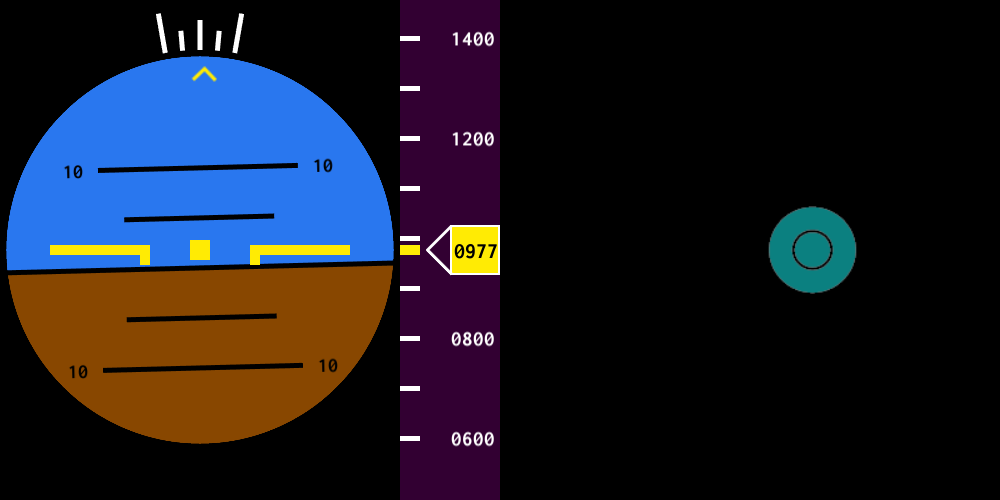
\includegraphics[width=0.8\linewidth]{figures/Aircraft/image1.png}
        \caption[The user interface]{The user interface consisting of the attitude indicator, altimeter, and secondary task.}
        \label{figure-hfes:userinterface}
    \end{center}
\end{figure}

\begin{figure}[b!]
    \begin{center}
        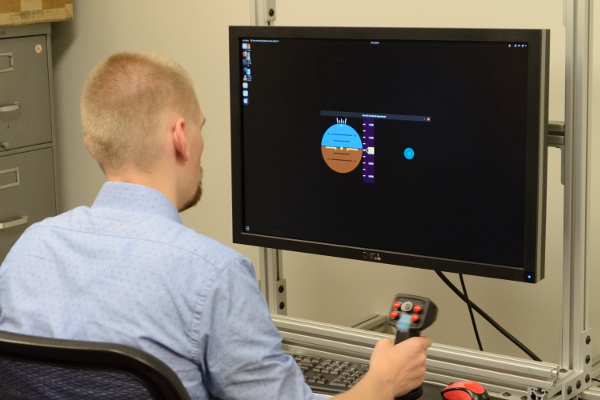
\includegraphics[width=0.8\linewidth]{figures/Aircraft/image2.png}
        \caption[A participant seated in front of the simulator display]{A participant seated in front of the simulator display, controlling the flight task with the joystick.}
        \label{figure-hfes:participant}
    \end{center}
\end{figure}

Participants were seated at a fixed-base simulator for the duration of the experiment, see Figure~\ref{figure-hfes:participant}.
The simulator consisted of a 30-inch monitor and a single joystick.
The user interface was centered in the display and presented to the user at 1000x500 pixels.
The user interface consists of a traditional aircraft attitude indicator on the left, an altimeter in the middle, and the secondary task on the right.
The Boeing 747 was modeled using data available in NASA CR-2144~\citep{heffley1972aircraft}.
Flight Condition 2 was chosen for this experiment, and represents slow, sea-level flight, with the landing gear retracted and with flaps extended to 20 degrees.
Longitudinal and lateral body axis derivatives were converted to the stability axis and implemented in a state-space model~\citep{stevens2015aircraft}.
The values from NASA CR-2144 for this flight mode were plugged into the longitudinal and lateral dynamics matrices presented in Appendix~\ref{appendix:dynamics}.
Participants used the elevators and ailerons to control pitch and roll, respectively.
Altitude was controlled by the subject with time-integrated pitch commands, as in a real aircraft.

\subsection{Experimental Design}
Participants were evenly split into two groups: a control group and a feedback group.
Participants in the feedback group received concurrent bandwidth feedback on the first 27 trials (9 in each control mode) and then flew the last 9 trials (3 in each control mode) without feedback to test their immediate retention.
Participants in the control group never received concurrent bandwidth feedback, nor was it mentioned to them during the study.

For participants experiencing feedback, feedback was presented based on the flight control mode of their current trial.
This feedback was implemented by changing the color of an indicator's elements from yellow to red when it deviated from outside of its allowed bandwidth and returning the indicator to yellow when it returned within the bandwidth.
Acceptable bandwidths of 3 degrees for pitch and roll, and 30 feet for altitude were chosen based on preliminary testing.
The choice of these bandwidths was based on preliminary pilot studies, and is further explored in Chapter~\ref{chapter:bandwidthstudy}.
Pitch feedback occurred on the center dot.
Roll feedback was shown on the wings and the roll indicator at the top of the attitude indicator.
Altitude feedback was enabled on the background color of the altimeter.
In Figure~\ref{figure-hfes:userinterface}, all three parameters are shown inside the acceptable bandwidth, and are therefore displayed in yellow.

Participants began the experiment by signing a consent form, then filled out a survey with demographic questions, then had a brief, pre-recorded training session.
After this training, participants immediately began the experiment and progressed through the 36 trials at their own pace.
Participants noted their workload on a piece of paper after each trial.
Subjects in the feedback group were paused after the 27th trial, at which time the proctor explained that the feedback would no longer appear, but that they ``should continue to perform the task to the best of [their] ability.'' Subjects in the feedback group also filled out a questionnaire after the end of the experiment trials which asked them about their experience with the feedback.

\subsubsection{Independent variables}
The three independent variables in this experiment were Group, Mode, and Trial.
Group, a between subjects factor, described if subjects received feedback --- Control or Feedback.
Mode, a within subjects factor, was the three different control modes --- P, PR, or PRA.
Trial, also a within subjects factor, was the trial that subjects repeated 12 times in each mode.

\subsubsection{Dependent measures}
The root-mean-square error (RMSE) of pitch was calculated for every trial.
This allowed for a consistent measurement across every trial as the same pitch disturbance was present regardless of the control mode.
The roll RMSE was calculated for each PR and PRA trial, and the altitude RMSE was calculated for each PRA trial.
The RMSE values provide an objective measurement of performance.
The secondary task was activated ten times per trial.
Participants had five seconds to correctly respond to the secondary task once it changed color.
We recorded the rates for correct and incorrect responses, as well as lack of response.
We used the average correct response time as objective indication of workload.
The Modified Bedford Workload Scale is a ten-point subjective workload measurement tool~\citep{roscoe_subjective_1990}.
Participants were asked to follow the scale and record their workload after each trial, allowing us to observe changes in workload during training.

\subsection{Hypotheses}
We had three major hypotheses for this experiment:
\begin{itemize}
    \item[\textbf{H1.}] Participants in the feedback group will immediately outperform those in the control group. We expect this effect to be most pronounced for the most complex mode and to see little to no improvement for simple trials.
    \item[\textbf{H2.}] Participants in the feedback group will have lower workload than participants in the control at the end of the experiment. We expect this effect to be most pronounced for the most complex mode and to see little to no improvement for simple trials.
    \item[\textbf{H3.}] Participants in the feedback group will not suffer from the guidance hypothesis and will retain their performance and workload levels when the feedback is removed in the immediate retention trials.
\end{itemize}
These hypotheses were established from the literature, our previous experiments with feedback, and early pilot studies with this simulation framework.

\section{Results}
\subsection{Participants}
Participants in the experiment were 30 engineering students from the University of California, Davis (23 men, M = 23.0 years, SD = 4.4; 7 women, M = 22.6 years, SD = 3.0).
All participants had normal or corrected-to-normal vision and full motor control of their upper bodies.
Eighty percent of participants had previously used a joystick, 43\% had spent time in flight simulators, and 30\% had prior flight experience.
Both gender and participants with flight experience were counterbalanced between the two groups.
Written informed consent was obtained prior to testing in accordance with the University of California, Davis Institutional Review Board (1399789-1).

\subsection{Analysis}
Mixed models were used to calculate the significance of factors in our analysis due to the presence of performance outliers which were removed from the analysis.
The Satterthwaite method was used to calculate the adjusted degrees of freedom using the lmerTest package in R~\citep{RN53}.
When significant effects were observed, post hoc comparisons using the Tukey Honest Significance Difference (HSD) test were performed and considered significant at the p $<$ .05 level, and the Satterthwaite method was again used to calculate the degrees of freedom.
Only 7 of the 1080 total trials (30 subjects with 36 trials per subject) were removed.
These trials were extreme performance outliers, and including these trials does not change the primary results of the study.
A three-factor (Group, Mode, and Trial) mixed model with two repeated measures (Mode and Trial) was run on the pitch root-mean-square error.
There were significant main factors of group ($F(1, 27.97) = 6.3, p = 0.018$), mode ($F(2, 53.47) = 29.7, p < .001$), and trial ($F(11, 300.29) = 48.4, p < .001$).
There were also significant interaction effects between group and trial ($F(11, 300.29) = 2.5, p < 0.01$) and between mode and trial ($F(22, 601.58) = 2.8, p < .001$).
Despite the presence of interaction effects that result from participants learning the task (as indicated by the trial factor), the main effects can still be interpreted, see Figure~\ref{figure-hfes:pitchrmse}.
A Tukey test showed that the participants in the groups differed significantly, with the participants in the feedback group outperforming those in the control group ($M = 2.35, 3.05$, respectively, $SE = 0.20$).
An additional Tukey test showed that the participants' performance in the modes differed significantly, and participants performed best in P mode, followed by the PR mode, and finally the PRA mode ($M = 2.30, 2.67, 3.14$ respectively, $SE = 0.15$).

This same analysis was completed on the roll root-mean-square error, with similar results.
There were significant main factors of group $(F(1, 28.00) = 8.8, p < 0.01)$, mode $(F(1, 27.93) = 6.8, p = 0.015)$, and trial $(F(11, 308.22) = 19.6, p < .001)$.
There was also a significant interaction effect between mode and trial $(F(11, 308.06) = 4.6, p < .001)$, see Figure~\ref{figure-hfes:rollrmse}.
Tukey tests showed that the participants' performance between the groups and the modes each differed significantly, with the participants in the feedback group again outperforming those in the control group ($M = 1.96, 2.43$, respectively, $SE = 0.11$), and performance was best in the PR mode followed by the PRA mode ($M = 2.15, 2.24$, respectively, $SE = 0.08$).
A two-factor (Group and Trial) mixed model with one repeated measure (Trial) was run on the altitude root-mean-square error.
There were significant main factors of group ($F(1, 27.54) = 5.2, p = 0.030$) and trial ($F(11, 301.57) = 11.4, p < .001$).
Tukey tests showed that the participants' performance between the groups differed significantly, with the participants in the feedback group again outperforming those in the control group ($M = 28.3, 50.2$, respectively, $SE = 6.8$), and the trial effect showing learning throughout the experiment for both groups, see Figure~\ref{figure-hfes:altitudermse}.
See Figure~\ref{figure-hfes:completermse} for a plot of the root-mean-square error for each flight task in each mode.
A three-factor (Group, Mode, and Trial) mixed model with two repeated measures (Mode and Trial) was run on the modified Bedford workload scores.
There were significant main factors of mode ($F(2, 56) = 134.8, p < .001$), and trial ($F(11, 308) = 8.7, p < .001$), and a significant interaction effect between mode and trial ($F(22, 616) = 2.0, p < 0.01$).
Tukey tests showed that the participants' workload between the modes differed significantly, with workload lowest in P, then PR, and finally PRA ($M = 3.80, 4.99, 6.16$, respectively, $SE = 0.28$), and the trial effect representing slightly reduced workload throughout the experiment.

\begin{figure}[b!]
    \begin{center}
        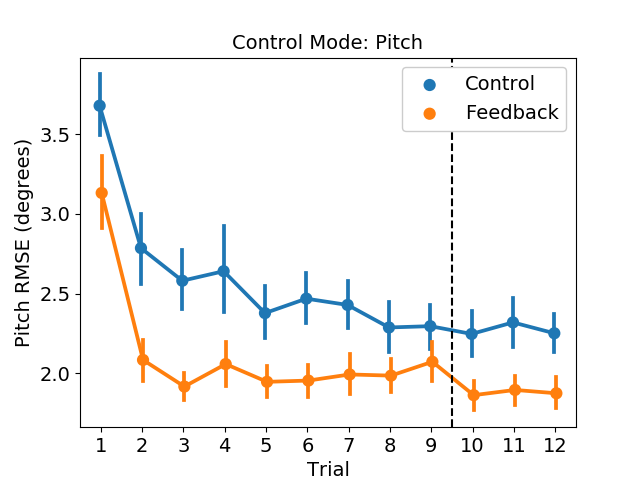
\includegraphics[width=0.8\linewidth]{figures/Aircraft/image3.png}
        \caption[The mean Pitch RMSE for each trial]{The mean Pitch RMSE for each trial for participants in the P control mode. Data points are the mean, and error bars are the standard error of the mean.}
        \label{figure-hfes:pitchrmse}
    \end{center}
\end{figure}
\begin{figure}[b!]
    \begin{center}
        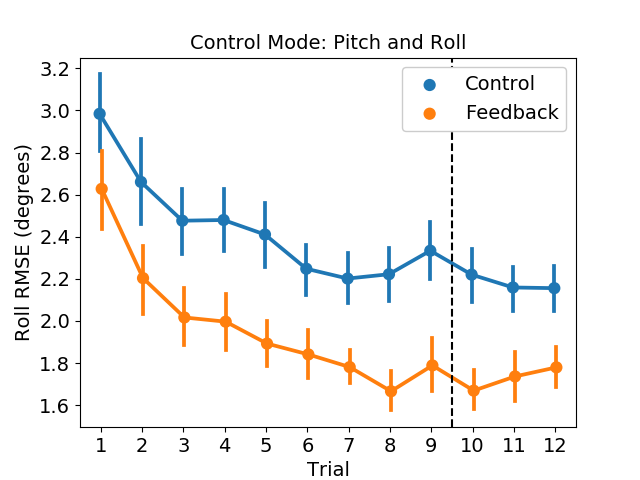
\includegraphics[width=0.8\linewidth]{figures/Aircraft/image4.png}
        \caption[The mean Roll RMSE for each trial]{The mean Roll RMSE for each trial for participants in the PR control mode. Data points are the mean, and error bars are the standard error of the mean.}
        \label{figure-hfes:rollrmse}
    \end{center}
\end{figure}
\begin{figure}[b!]
    \begin{center}
        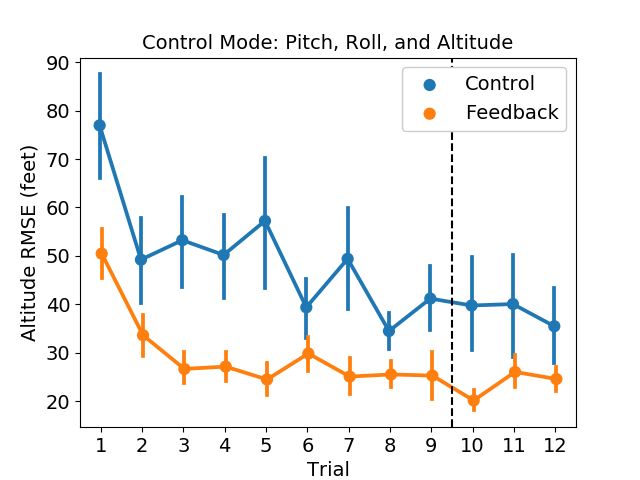
\includegraphics[width=0.8\linewidth]{figures/Aircraft/image5.png}
        \caption[The mean Altitude RMSE for each trial]{The mean Altitude RMSE for each trial for participants in the PRA control mode. Data points are the mean, and error bars are the standard error of the mean.}
        \label{figure-hfes:altitudermse}
    \end{center}
\end{figure}

\begin{figure}[b!]
    \begin{center}
        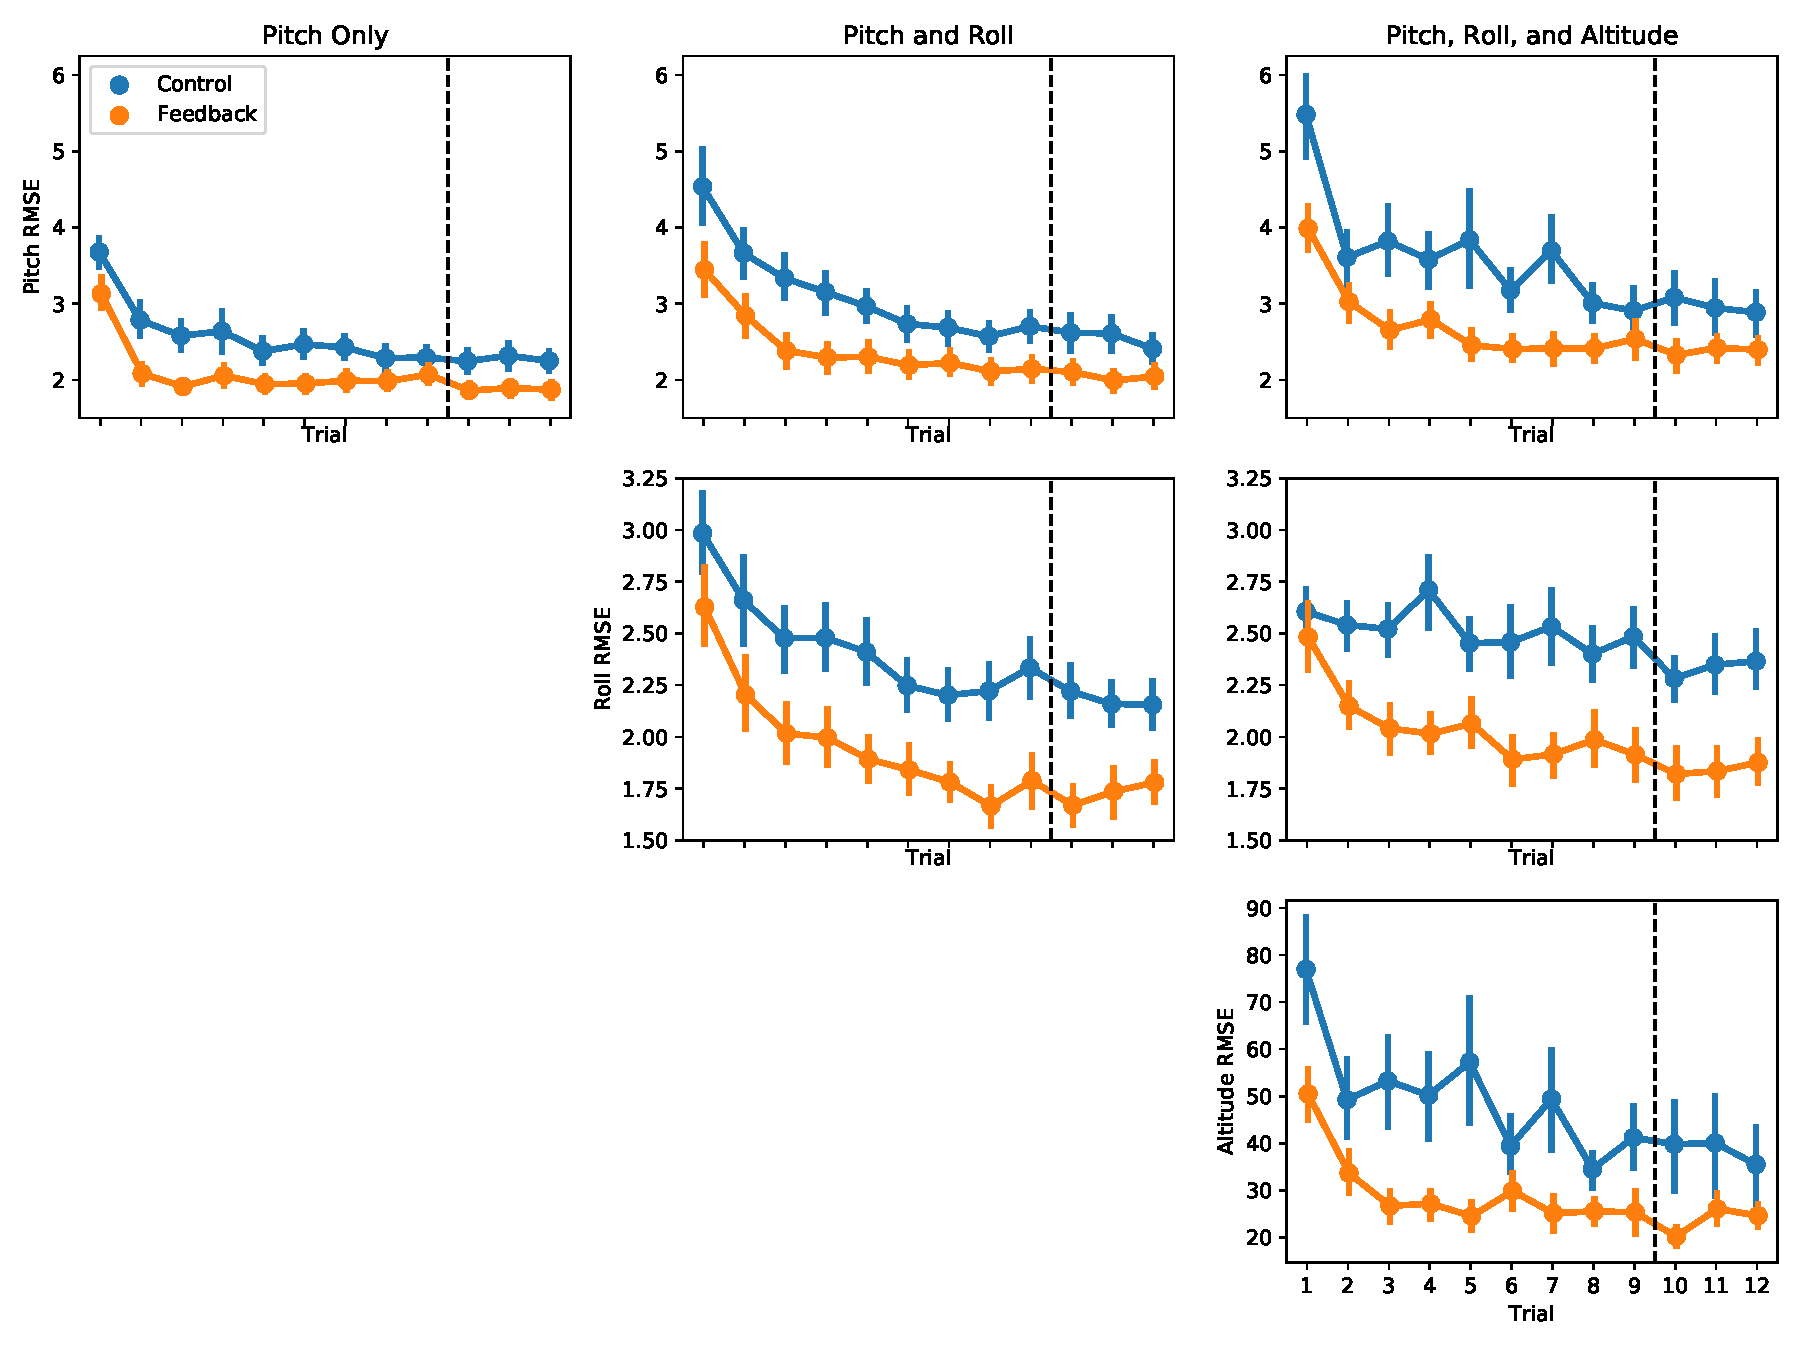
\includegraphics[width=\linewidth]{figures/Aircraft/performance_measures.pdf}
        \caption[The root-mean-square error for each flight task in each mode]{The root-mean-square error for each flight task in each mode. Data points are the mean, and error bars are the standard error of the mean.}
        \label{figure-hfes:completermse}
    \end{center}
\end{figure}

\section{Discussion}

\begin{table}[tb]
    \centering
    \includetable{aircraft-perf-improvement.tex}
    \caption[Performance improvement of the feedback group over the control group]{Performance improvement of the feedback group over the control group at the end of the experiment for each flight RMSE metric.}
    \label{aircraft:perf-improvement}
\end{table}

Our analysis showed that participants in the feedback group performed significantly better than the control group in every trial across every metric and flight control mode.
For the first time that participants completed P, PR, and PRA trials, the feedback group performed 17.5\%, 31.7\%, and 37.4\% better than the control group according to the pitch RMSE metric.
Participants in the feedback not only immediately performed better, they also reached their peak performance much faster and had a final performance level which was significantly better than the control group, see Table~\ref{aircraft:perf-improvement}.
The largest performance improvement was seen in controlling altitude, where the feedback group had a final performance level which was 44.2\% better than the control group, confirming H1.
No group-related workload differences were detected in either the Modified Bedford scores or in the secondary task reaction times.
This suggests that, for tasks of this complexity, concurrent bandwidth feedback may not reduce workload~\citep{karasinski_evaluating_2019}.
Thus, for our second hypothesis, H2---we find that concurrent bandwidth feedback does not reduce workload in our flight tasks, and that tasks with higher functional complexity may be required to observe these effects.
Our third hypothesis was that subjects would primarily use the concurrent bandwidth feedback as a learning tool but that they would not become dependent on the feedback to the point that they required it to complete the task.
Retention tests are commonly used in the augmented feedback literature to verify that participants are not dependent on the feedback techniques.
Our analysis indicates no significant performance changes across any of our performance metrics when the feedback was removed, confirming H3.
After the experimental trials, we asked participants in the feedback group to complete a survey designed to identify when the feedback was or was not useful and how participants thought their performance and workload changed in the retention phase of the experiment.
One hundred percent of participants thought that the feedback helped them perform the task, 80\% reported that it helped them regain focus when their mind wandered, 73\% reported that it helped them to learn a scan pattern, and 27\% reported that the feedback was motivating.Survey results suggested that participants found the feedback especially useful in the roll and altitude tasks, which was reflected in the objective performance metrics.

\section{Conclusions}
Participants took part in a study investigating the effect of concurrent bandwidth feedback on flight performance and workload in three flight control modes of increasing complexity.
The participants in the feedback group performed significantly better than those in the control group, generally performing better on their second trial than those in the control group could by the end of the experiment.
Subjective and objective workload metrics showed no change in participant workload between the groups.
Survey questions identified that most participants found the feedback helpful in training them to establish a scan pattern, helping them to learn the task much quicker than those without feedback.
Feedback was removed for immediate retention trials, and participants showed no changes in performance or workload, suggesting that participants did not suffer from the guidance hypothesis.

\chapter{Feedback Bandwidth Study}
\label{chapter:bandwidthstudy}

\section{Introduction}

As we mentioned in Section~\ref{section:cbf}, several authors have noted that ``[b]andwidth feedback has been shown to be effective; however, setting the error threshold is not trivial''~\citep{timmermans_technology-assisted_2009, RIBEIRO2011231, sigrist_augmented_2013}.
While choosing to use an operational limit of acceptable performance can make the choice of setting the error threshold simpler, this option is not always available.
Additionally, mission designers often want to know what the optimum pilot performance is for mission planning, and instructors are interested in what levels of performance are acceptable during training.

Our previous work has shown that concurrent bandwidth feedback can be effective, but our choice of bandwidth has been ad-hoc in nature and primarily based on preliminary pilot studies.
These pilot studies have shown that there may be a wide variety of acceptable bandwidths, but it is unclear if there is a single bandwidth that would lead to optimal performance or a minimum learning time.
It is clear, however, that adverse thresholds which require unrealistic performance will not improve performance and may lead to degraded performance when compared to a no feedback condition.
Bandwidths that are too loose or not demanding enough will result in feedback that is sparse and may result in performance that resembles a no feedback condition.

\section{Method}

We designed a follow-up experiment to the experiment presented in Chapter~\ref{chapter:aircraftfeedback} which investigates the changes in performance that result from exposure to different bandwidths.
This experiment uses the same simulator and flying task as the previous experiment with a few changes.
The display, forcing functions, and secondary task were all identical to the previous experiment.
In this experiment, however, subjects only completed trials in the pitch and roll mode.

\subsection{Experimental Design}

In this experiment, subjects were randomly assigned to one of four groups.
These consisted of a control group, which received no feedback, and three feedback groups which received feedback during training.
Subjects in the feedback groups received concurrent bandwidth feedback along both the pitch and roll axes at 2, 3, or 4 degrees.
As with the previous experiment, the feedback on each axis was activated independently when the individual axis crossed over the threshold bandwidth.
Unlike the previous experiment, which only had a training and immediate retention phases, this experiment has four phases spread across two experiment sessions.
During the first session subjects completed 16 training trials followed by 8 immediate retention trials, during which time subjects in feedback conditions had their feedback removed.
Subjects were dismissed after completing the immediate retention trials and asked to return approximately 24 hours later for the second experiment session.
In the second session, subjects completed 8 retention trials without feedback, then completed 8 transfer task trials without feedback.
The only change between the transfer task and the other trials is the system dynamics of the controlled vehicle and the magnitude of the disturbance force.
In the transfer task, subjects were responsible for flying a Navion aircraft instead of a Boeing 747.
The Navion was modeled using data available in NASA CR-96008~\citep{teper1969aircraft}.
Compared to the Boeing 747, the Navion is a much smaller and lighter aircraft, which requires a significantly different control strategy to effectively control.
The disturbance force consisted of the same functions as in the rest of the experiment but was scaled down such that maximum pitch deflection under an uncontrolled scenario was approximately the same as with the Boeing 747 trials.

\subsubsection{Independent variables}
The two independent variables in this experiment were Group and Trial.
Group, a between subjects factor, described if and when subjects received feedback.
Trial, a a within subjects factor, was the trial that subjects repeated over the course of the experiment.

\subsubsection{Dependent measures}
The root-mean-square error (RMSE) of pitch and roll was calculated for every trial and provided an objective measurement of performance.
As in the previous experiment, the secondary task was activated ten times per trial and participants had five seconds to correctly respond to the secondary task once it changed color.
We used the average correct response time as objective indication of workload.
Participants were asked to follow the Modified Bedford scale and record their workload after each trial, allowing us to observe changes in workload during training.

\subsection{Hypotheses}
We had four hypotheses for this experiment:
\begin{itemize}
    \item[\textbf{H1.}] Participants in the feedback groups will immediately outperform those in the control group.
    \item[\textbf{H2.}] Participants will report the same workload between groups, which will gradually decrease with training.
    \item[\textbf{H3.}] Participants in the feedback group will not suffer from the guidance hypothesis and will retain their performance and workload levels when the feedback is removed in the immediate retention and 24 hour retention trials.
    \item[\textbf{H4.}] Participants will continue to perform at relatively similar levels when they complete the transfer task.
\end{itemize}

\section{Results}
\subsection{Participants}
In December 2019, coronavirus disease 2019, commonly referred to as COVID-19, began to spread and quickly resulted in a global pandemic.
COVID-19 is an infectious disease caused by severe acute respiratory syndrome coronavirus, is highly contagious, and is mainly spread during close contact.
As a result of this pandemic, the University of California, Davis was closed and the Institutional Review Board recommended that we act to ``limit transmission of the virus by delaying or otherwise modifying non-essential interactions,'' postponing subject testing.
We had anticipated testing approximately 10-15 subjects per group, for a total of 40-60 subjects.
The remainder of the results discussed here are preliminary and based on the 19 subjects whose data was collected before a shelter-in-place was ordered.

Participants in the experiment were 19 engineering students from the University of California, Davis (17 men, 1 woman, 1 decline to state) with an average age of 21.3 years (SD = 2.2).
All participants had normal or corrected-to-normal vision and full motor control of their upper bodies.
Both gender and participants with flight experience were counterbalanced between the two groups.
Of the 19 subjects, 18 returned the next day after an average of 24.93 hours (SD = 0.6).
This study was exempted by the University of California, Davis Institutional Review Board, and subjects were not compensated for their time.

\subsection{Analysis}

As in the previous study, mixed models were used to calculate the significance of factors in our analysis due to the presence of performance outliers which were removed from the analysis and the Satterthwaite method was used to calculate the adjusted degrees of freedom using the lmerTest package in R.
When significant effects were observed, post hoc comparisons using the Tukey Honest Significance Difference (HSD) test were performed and considered significant at the p $<$ .05 level, and the Satterthwaite method was again used to calculate the degrees of freedom.
A two-factor (Group and Trial) mixed model with one repeated measures (Trial) was run on the pitch root-mean-square error.
There was a significant main factor of trial ($F(31, 434) = 3.6, p < 0.001$) and group was not significant ($F(3, 14) = 2.6, p = .09$).
Additionally, the interaction effect between group and trial was not significant ($F(93, 434) = 0.9, p = 0.78$).
This result indicates that subjects learned to perform the task over time but that the effect of group was not significant given the effect size and current number of subjects.
Even with one half to one third of the anticipated number of subjects, however, the main effect of group is already heading towards significance, as we would expect based on the results of the previous study.
Differences in groups are beginning to emerge when examining the plot, see Figure~\ref{figure-bw:pitchrmse}, though the error bars are too large to draw definite conclusions.

This analysis can also be performed on the other dependent measures, with similar results.
Most metrics closely track those seen in the previous study, though the low sample size makes it difficult to draw conclusions.
Due to their extremely preliminary nature, these results are not included here.

\begin{figure}[tb!]
    \begin{center}
        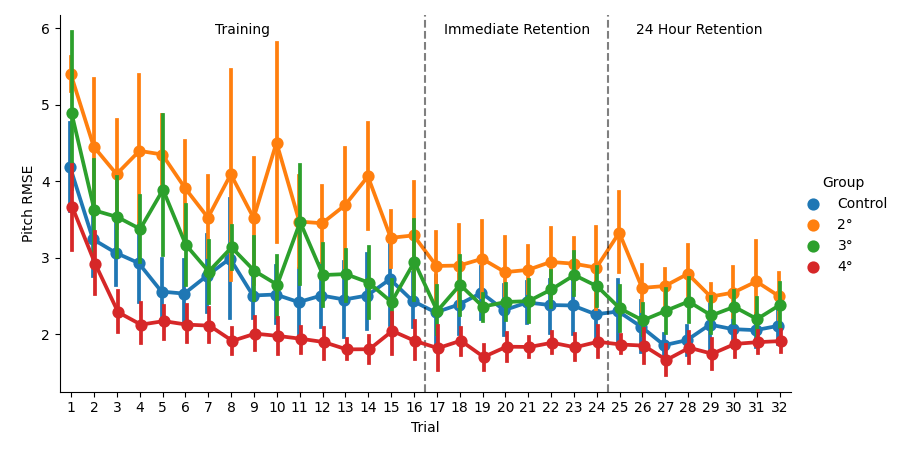
\includegraphics[width=\linewidth]{figures/Aircraft/Bandwidth-PitchRMSE.png}
        \caption[The mean Pitch RMSE for each trial]{The mean Pitch RMSE for each trial for participants. Data points are the mean, and error bars are the standard error of the mean.}
        \label{figure-bw:pitchrmse}
    \end{center}
\end{figure}

\section{Discussion}

Based on the preliminary findings presented in Figure~\ref{figure-bw:pitchrmse}, choosing an appropriate bandwidth can potentially have an effect of the efficacy of concurrent bandwidth feedback.
While we have yet to observe statistically significant effects, current data suggests that having a looser bandwidth improves performance.
While it was expected that there may be an optimal choice of bandwidth to maximally reduce training times and improve performance, we hypothesized that this value would be lower than or approximately equal to three degrees, not a higher value, based off our pilot studies.

While we cannot make any definite claims based on this preliminary data and analysis, we can revisit data from the previous experiment to make further predictions.
Increasing the acceptable bandwidth of feedback results in the concurrent bandwidth feedback being presented less often, and the repetition allowed for in training results in subjects improving their performance and reducing their deviations during compensatory tracking.
We can use the disturbance force to estimate the percentage of time that subjects are exposed to the feedback as we presented subjects with the same disturbance force during each trial.
Figure~\ref{figure-bw:pitchfeedback} presents the percentage of time that pitch feedback would be active if subjects did not provide any control input whatsoever.
This suggests that at the beginning of training subjects with a bandwidth of two, three, and four degrees would experience feedback 76\%, 62\%, and 47\% of the time, respectively, if they provided no input.

Subjects in the feedback group had their bandwidth set at three degrees in our previous experiment and were instructed to try and improve their performance whenever they saw that the feedback was activated.
By looking at the percentage of pitch errors that were above a given value, we can infer what percentage of time feedback would have been on when subjects had finished their training phase, regardless of chosen bandwidth.
Figure~\ref{figure-aircraft:pitchfeedback} presents the percentage of time that pitch feedback was active at the end of training, showing 12\% for the three-degree bandwidth subjects experienced.
It is unclear if subjects continue to improve until they reach a point where feedback appears approximately 12\% of the time, or if this is simply a limit of human motor control for this task.
In either case, the 4\% of time feedback would have been presented if a four-degree bandwidth was chosen is clearly within human control.
If the 12\% target is a true motivational limit, 4\% would likely inspire greater confidence in subjects, who may go on to report lower workload values.
The two-degree bandwidth, however, would only be attainable 29\% of the time by fully trained subjects in the previous experiment, and would likely have a demotivating or otherwise negative effect.

\begin{figure}[tb!]
    \begin{center}
        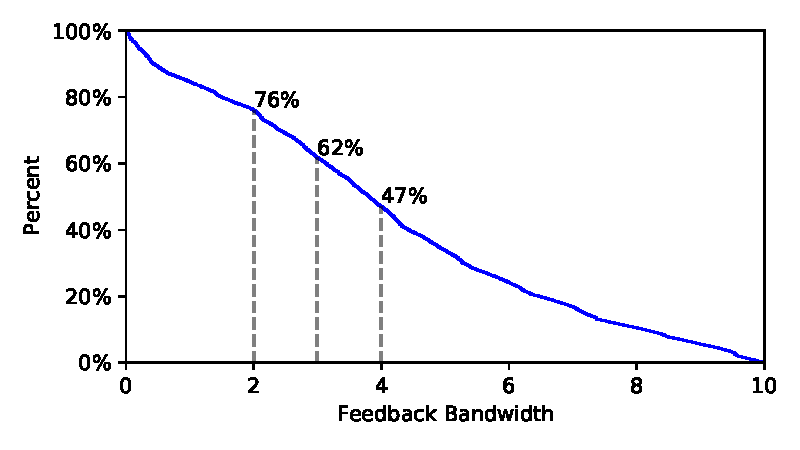
\includegraphics[width=\linewidth]{figures/Aircraft/no_input_feedback_on.pdf}
        \caption[The mean percentage of active pitch feedback with no input present]{The percentage of active pitch feedback with no input present. This represents the resulting aircraft motion due to the disturbance force.}
        \label{figure-aircraft:noinput_pitchfeedback}
    \end{center}
\end{figure}
\begin{figure}[tb!]
    \begin{center}
        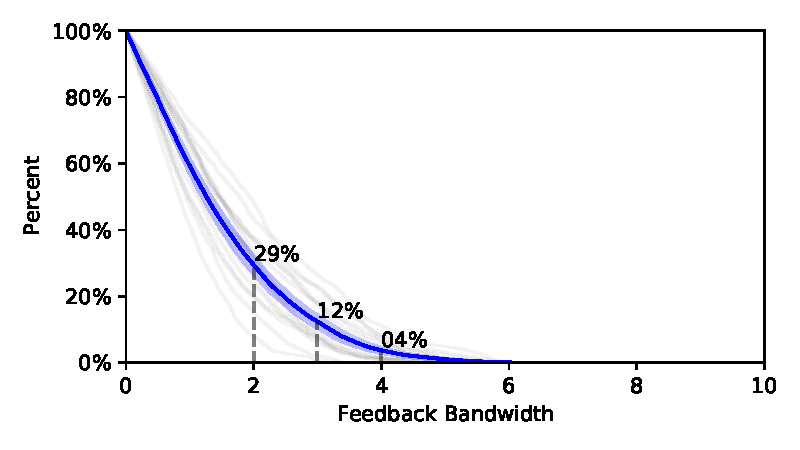
\includegraphics[width=\linewidth]{figures/Aircraft/p34_feedback_on.pdf}
        \caption[The mean percentage of active pitch feedback time at the end of the previous study]{The percentage of active pitch feedback time at the end of the previous study, when the bandwidth was set to three degrees. Data points are the mean, and the shaded region is the standard error of the mean.}
        \label{figure-aircraft:pitchfeedback}
    \end{center}
\end{figure}
\begin{figure}[tb!]
    \begin{center}
        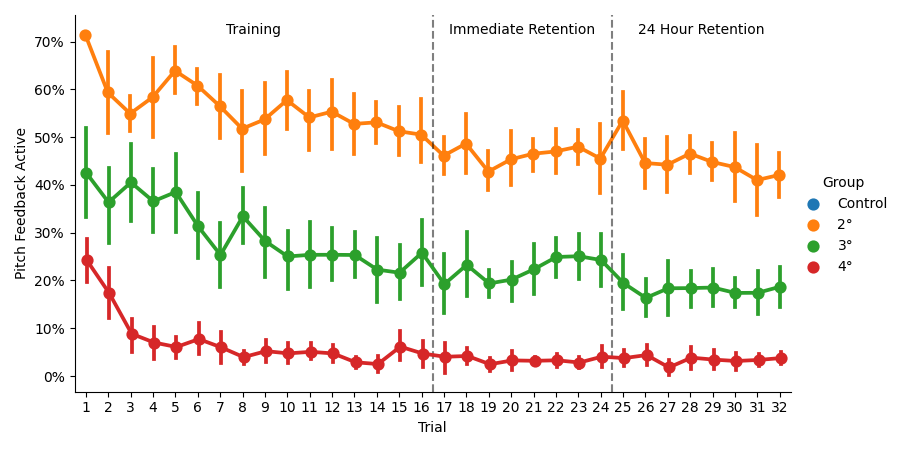
\includegraphics[width=\linewidth]{figures/Aircraft/Bandwidth-PitchFeedbackOn.png}
        \caption[The mean percentage of active pitch feedback time for each trial]{The percentage of active pitch feedback time for each trial for participants. Data points are the mean, and error bars are the standard error of the mean.}
        \label{figure-bw:pitchfeedback}
    \end{center}
\end{figure}

Finally, we can take a preliminary look at how often subjects in this experiment experienced their feedback between the different bandwidth groups.
The percent of time that feedback was active at the beginning and end of training should provide some insight into how subjects respond to different bandwidth levels.
Figure~\ref{figure-bw:pitchfeedback} should the percentage of active feedback time for each trial for subjects in the three feedback groups.
We can see how effectively subjects used the feedback on the first trial by looking at the difference between the value on this plot and that predicted by the no feedback case.
On the first trial, subjects in the three feedback groups tended to reduce their anticipated feedback exposure more the larger the bandwidth was.
Subjects in the four-degree bandwidth group, for instance, nearly halved their anticipated feedback exposure, as could be expected from their pitch RMSE presented in Figure~\ref{figure-bw:pitchrmse}.
Additionally, subjects in this group asymptote very close to the 4\% value predicted by subjects in the previous study.
The two- and three-degree bandwidth groups, however, continue to show much larger feedback exposure percentages.
The results for subjects in the three-degree bandwidth group are especially confusing, as they do not asymptote to the 12\% number shown by subjects in the previous experiment.
While the differences in experimental procedures could be the cause of this, we believe that the low sample size (5 subjects thus far in this experiment compared to 15 subjects in the previous experiment) are more likely the cause.

\section{Conclusions}
While the preliminary data collected for this experiment can be used to begin to explain the effects of using different bandwidths in concurrent bandwidth feedback, more subjects are needed to make definitive claims.
Briefly revisiting our hypotheses, we can begin to predict the results of this study.
\begin{itemize}
    \item[\textbf{H1.}] While subjects in the three- and four-degree bandwidth groups will likely immediately outperform those in the control group, the two-degree bandwidth presents too much of a challenge for subjects to effectively use the concurrent bandwidth feedback.
    This indicates that researchers should be careful to choose attainable bandwidths, or they may incorrectly conclude that concurrent bandwidth feedback, in general, does not work for their task.
    \item[\textbf{H2.}] Based on our early results, participants will report the same workload between groups, which will gradually decrease with training.
    \item[\textbf{H3.}] Participants in the feedback group will not suffer from the guidance hypothesis and will retain their performance and workload levels when the feedback is removed in the immediate retention and 24 hour retention trials.
    \item[\textbf{H4.}] It is still too early to make claims on the effects of concurrent bandwidth feedback on transfer of training.
\end{itemize}
Finally, we note that this study will resume testing when the University of California, Davis Institutional Review Board deems that testing can continue.
% This work will provide valuable insight into the effect of choosing an appropriate bandwidth for training motor control tasks.

\chapter{Modeling the Effects of Feedback}
\label{chapter:modeling}

% % Outline
% Introduction
% Method
%     The Task
%     Modeling Techniques
%         ARX
%         Structural Model
% Results
%     ARX
%         full wc results
%     SM
%         wc results for pitch only
%         differences between groups
%     Comparison
%         of wc results
% SM Model Extension
%     Ke is diff, add new Kf parameter
% Discussions

\section{Introduction}
\textbf{\color{red} This chapter discusses the last of my PhD work.
    The work is approximately 90\% complete, but the final results and writeup are not yet complete.}

\subsection{Motivation}
The second Aim of this dissertation is to develop a model of the human pilot which includes the effects of concurrent bandwidth feedback.
The model presented here extends Hess' Structural Model of the human pilot.
The Structural Model has been extremely successful in predicting human performance through a variety of system dynamics and can predict how performance changes during a pilot's adaptation to changing dynamics.
Hess has developed adaptive logic for the human pilot in a pursuit task which triggers when the pilot notices that vehicle dynamics have changed~\citep{hess_modeling_2009}.
This logic is based off several criteria, which ``must be predicated upon information available to the human [and] the postadapated pilot models must follow the dictates of the crossover model of the human pilot''~\citep{hess_modeling_2009}.
The primary result of the adaptive logic is to increase the resulting crossover frequency of the pilot, effectively making them more responsive, which could be interpreted as more focused on the task.

\begin{figure}[tb]
    \begin{center}
        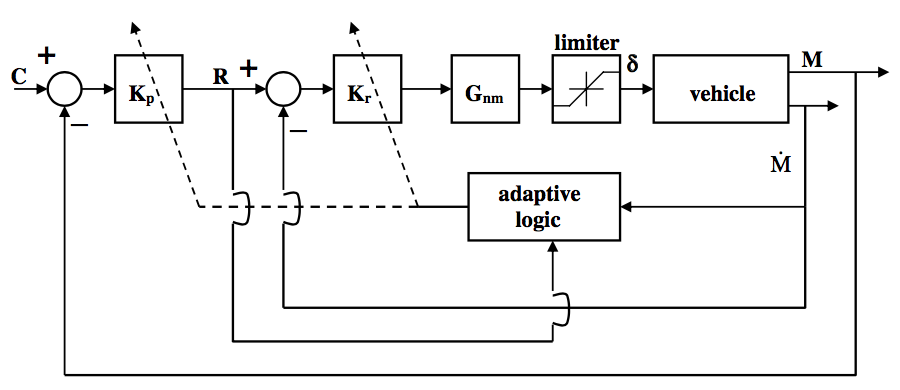
\includegraphics[width=0.8\linewidth]{figures/Modeling/Screen_Shot_2018-08-09_at_4_15_24_PM.png}
        \caption[Hess' model of the adaptive human pilot]{Hess' model of the adaptive human pilot, from~\citet{hess_modeling_2009}.}
        \label{figure:hesspursuit}
    \end{center}
\end{figure}

While this model of the adaptive pilot has been successful in predicting changes in performance for a well trained subject, it does not consider how a pilot would behave when they are still in the early stages of training.
The modified model presented here includes two major changes to Hess' current model:
\begin{itemize}
    \item The adaptation logic is changed to focus on concurrent bandwidth feedback
    \item The timescale of the adaptation is significantly longer
\end{itemize}

Here, the adaptive logic to triggers when the pilot is receiving concurrent bandwidth feedback, rather than when a change in system dynamics occurs.
This will requires the addition of a feedback loop onto the Structural Model which triggers when the bandwidth feedback is activated.
This loop is based around the $K_e$ gain, which is the primary way of setting the crossover frequency in the Structural Model.
This change implies that the subjects in our experiments do their primary learning when they are receiving qualitative feedback that their current level of aggressiveness is not sufficient to complete the task.

While there must be a separate loop that adjusts the crossover frequency as learning progresses over the course of several hours, the change in performance we see when subjects use the concurrent bandwidth feedback happens relatively rapidly, within a few minutes.
This is reflected in the delta of performance between subjects in the different groups of our SAFER experiment, even on the first trial, see Figure~\ref{figure:saferdistance}.
This relates to the second required change, the amount of required adaptation time.
Hess' model requires that pilots adapt within a very short time period, on the order of 5 seconds~\citep{weir_model_1966}.
The results of our experiment with SAFER and the three-axis tracking task also suggest relatively long adaptation times, on the order of a few minutes, again see Figure~\ref{figure:saferdistance}.

\section{Method}

\subsection{The Piloting Task}

\begin{figure}[b]
    \centering
    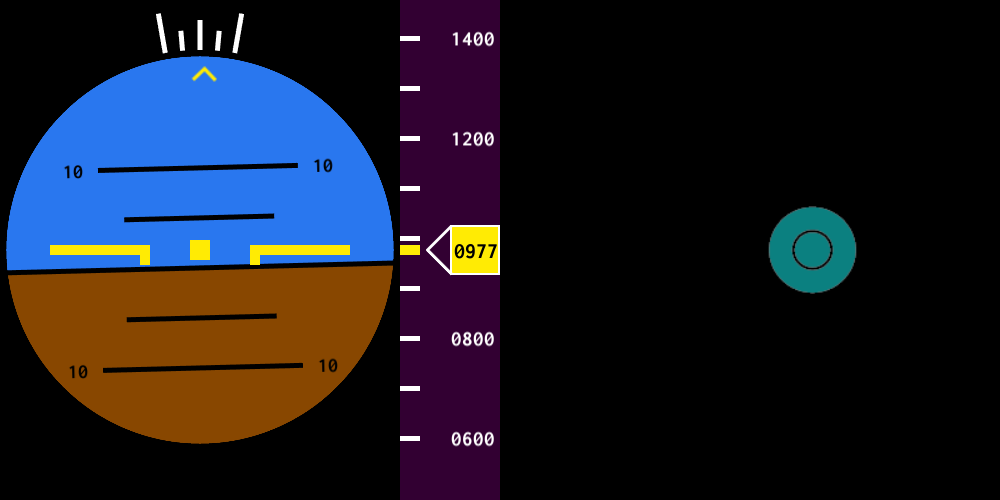
\includegraphics[width=0.8\linewidth]{figures/Aircraft/image1.png}
    \caption[The interface]{The interface that participants were presented with during the experiment, showing the flight task on the right with deviations from nominal in pitch, roll, and altitude, and the secondary, two-choice, task on the right.}
    \label{fig:display}
\end{figure}

Training operators to perform complex manual control tasks is expensive and time consuming, and poorly trained operators can cause catastrophic failures.
The use of concurrent feedback techniques has been shown to improve performance and reduce training times, but has not previously been evaluated for complex, real-world tasks such as flying aircraft.
In the experiment (fully described in Chapter~\ref{chapter:aircraftfeedback}), thirty participants were evenly split into two groups and tasked with flying a simulated Boeing 747 aircraft in three control modes of increasing degrees of freedom and functional complexity.
In order of increasing degrees of freedom and functional complexity, these three control modes were:
\begin{itemize}
    \item[\textbf{P}] Pitch only (low complexity)
    \item[\textbf{PR}] Pitch and Roll (moderate complexity)
    \item[\textbf{PRA}] Pitch, Roll and Altitude (significant complexity)
\end{itemize}
The control group controlled simulated aircraft motion with visual guidance for pitch, roll, and altitude provided by traditional flight instruments.
The feedback group received additional visual concurrent feedback for each controlled degree of freedom.
For both groups, performance measurements were evaluated to determine the effects of the feedback on subject learning rate and maximum skill level.
To assess short-term retention of learned skill for the feedback group, the concurrent feedback was removed, and performance was again evaluated.

Each participant completed a total of 36 trials; 12 in each of the three control modes.
Each trial had a duration of 82 seconds, and participants self-initiated the trial by activating a trigger on the joystick.
The complete results of this experiment can be seen in Chapter~\ref{chapter:aircraftfeedback}.

The two groups of participants are: control and feedback, and the interface that participants saw during the experiment is available in Figure~\ref{fig:display}.
When the vehicle was well controlled (small errors in the controlled degrees of freedom), the interface was the same for participants in both groups.
Depending on the control mode the the participant was completing, however, participants in the feedback group experienced concurrent bandwidth feedback on various elements of the attitude indicator and altimeter.
This feedback was indicated by changing the element from the default yellow color to a red color when the error deviated outside of a predetermined bandwidth.
Pitch feedback was provided on the central pitch indicator when the pitch was three or more degrees from zero, roll feedback was provided on the attitude indicator's ``wings'' when the roll was three or more degrees from zero, and attitude feedback was provided on the altimeter text box when the altitude was 30 feet or more off the nominal altitude of 1000 feet.
After the 9th trial, subjects in the feedback group no longer experienced feedback, and the interfaces for the control and feedback groups were the same.
This was done in order to investigate how well the subjects could retain their performance benefit.

\subsubsection{Experiment Results}
The resulting root-mean-square error for each group of participants by trial is presented in Figure~\ref{fig:prmse}.
Both groups of participants had a relatively high initial RMSE which was reduced through repeated training on the task.
Participants in the feedback group, however, performed significantly better than those in the control group and learned the task much faster.
Additionally, subjects in the feedback group were able to maintain their improved performance when the feedback was removed, and actually show a slight increase in performance when this occurs.

\begin{figure}[t]
    \centering
    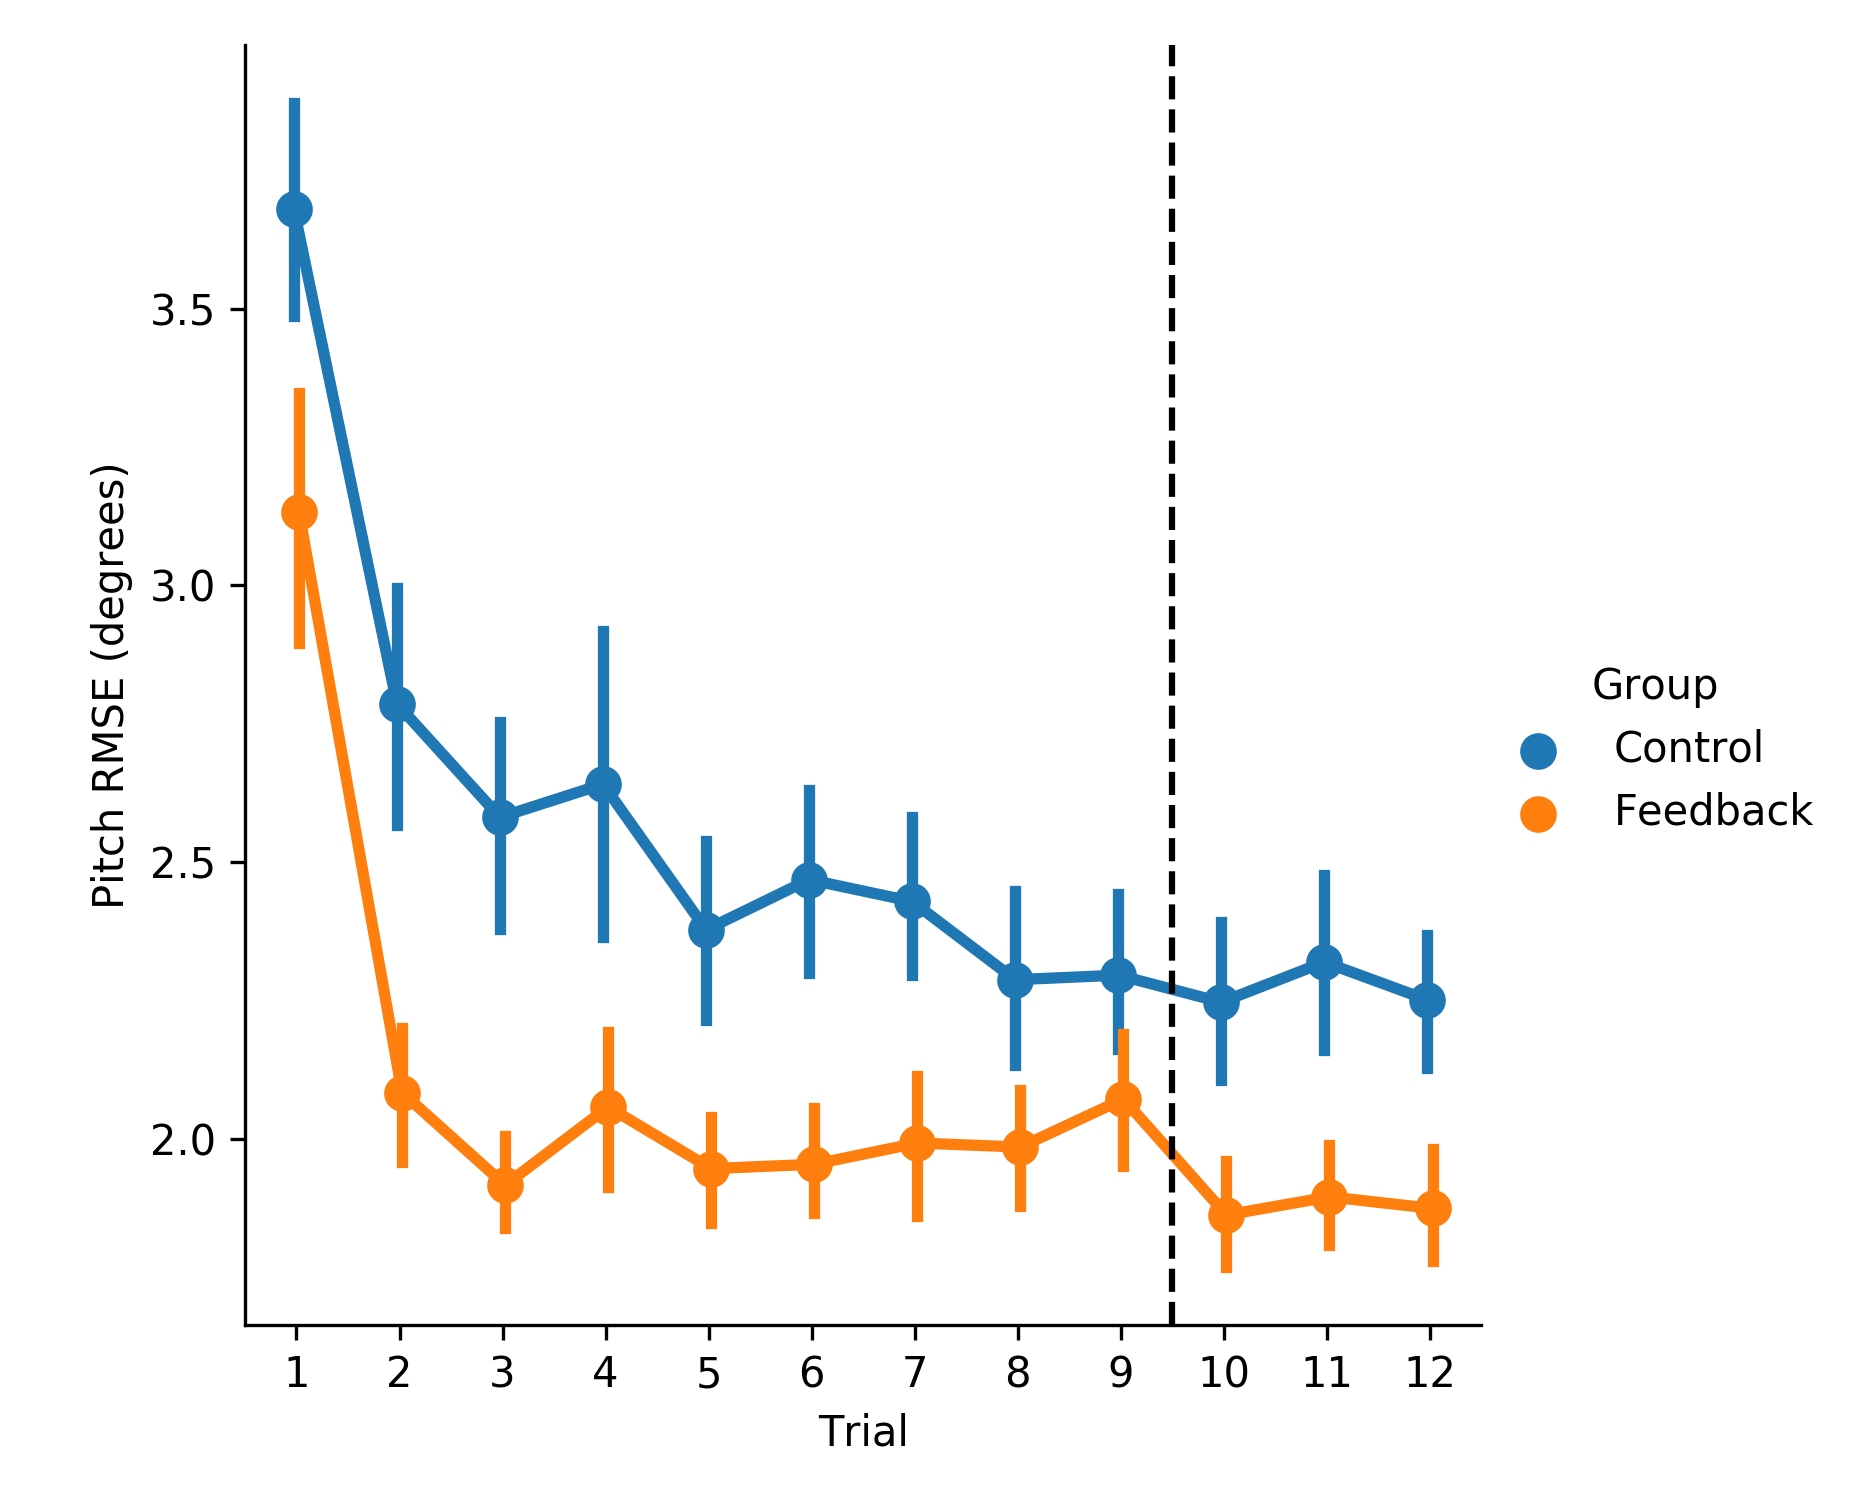
\includegraphics[width=0.8\linewidth]{figures/Modeling/prms_arx.png}
    \caption[Pitch root-mean-square error]{Pitch root-mean-square error. Feedback was removed from subjects in the feedback group after the 9th trial in order to investigate retention.}
    \label{fig:prmse}
\end{figure}

\subsection{Modeling Techniques}
We investigated two techniques for creating models of human pilot in order to better understand the results of the aircraft training study.
Both techniques produce an estimated transfer function of human operator, $Y_p$, which can be combined with the controlled system dynamics, $Y_c$, in order to explore the crossover model characteristics discussed in~\ref{background:pilotmodeling}.
The crossover frequency can be identified using
\begin{align}
    Y_c Y_p = \dfrac{w_c e^{-s \tau_e}}{s}
\end{align}
which provides an indication of how hard the operator is working.

\subsubsection{Autoregressive Model with Exogenous Variables (ARX)}
Autogregressive (AR) models are commonly used to represent time-varying processes in which an output variable linearly depends on its previous value and a stochastic error term.
When a process also depends on an input variable (often referred to as an exogenous variable), the resulting model is known as an autoregressive model with exogenous variables (ARX).
The structure of an ARX model is given by
% https://www.mathworks.com/help/ident/ref/arx.html
\begin{equation}
    y(t) + a_1 y(t-1) + \ldots + a_{n_a} y(t - n_a) = \\
    b_1 u(t-n_k) + \ldots + b_{n_b} u(t-n_b - n_k+1) + e(t)
\end{equation}
where $y(t)$ is the output variable at time $t$, $n_a$ is the number of poles, $n_b$ is the number of zeros, $n_k$ is the number of input samples which occur between input and output (also known as the dead time or time delay in the system), $y(t-1) \ldots y(t-n_a)$ are the previous outputs on which the current output depends, $u(t-nk) \ldots u(t-n_b - n_k+1)$ are the delayed inputs on which the current output depends, and $e(t)$ is a white-noise error term.

An autoregressive technique to identify a transfer function from an input/output time sequence pair was previously developed in~\citet{hess_modeling_2002}.
Using this technique, called \textit{gettf1}, we identified transfer functions representing pilot models for the data trials from our experiment.
The inputs to this technique are the input and output timeseries and $n_a, n_b,$ and $n_k$.
For the results presented in this Chapter, $n_a = n_b = 10$ and $n_k = 0$.
This technique uses an ARX model which is fit using least-squares, and results in a discrete transfer function model estimation of the input/output system.
The script also produces a continuous transfer function using a Tustin approximation.
The result of this process is a transfer function of the pilot with ten poles and zeros describing the human operator's response to the displayed flight dynamics.

\subsubsection{Structural Model}
This is more complicated, as there are many parameters to identify which interact nonlinearly, and the fit function has many local maximums.

\begin{figure}[t]
    \centering
    \begin{subfigure}[b]{\textwidth}
        \centering
        \includegraphics[width=0.8\textwidth]{figures/structural_model/structural_model.pdf}
        \caption[The Structural Model]{The Structural Model, adapted from~\citet{hess_unified_1997}.}
        \label{fig:structuralmodel}
    \end{subfigure}
    \hfill
    \begin{subfigure}[b]{\textwidth}
        \centering
        \includegraphics[width=0.8\textwidth]{figures/structural_model_reduced/structural_model.pdf}
        \caption[The reduced structural model used in this analysis]{The reduced structural model used in this analysis.}
        \label{fig:structuralmodelreduced}
    \end{subfigure}
    \caption[The Structural Model of the Human Pilot]{The Structural Model of the Human Pilot.}
    \label{fig:structuralmodels}
\end{figure}

The complete Structural Model in Figure~\ref{fig:structuralmodel} can be reduced to Figure~\ref{fig:structuralmodelreduced} by setting the following standard parameter values.

\begin{align}
    \nonumber    S_1 = S_2 = S_3 = \enspace \downarrow \\
    \nonumber    K_{\dot{e}} = \epsilon = K_{\dot{m}} = K_{\ddot{m}} = 0
\end{align}

These switches are set to their standard locations for normal error sensing~\citep{hess_unified_1997}.
$\epsilon$ is set to zero for simplicity.
$K_{\dot{m}}$ and $K_{\ddot{m}}$ are set to zero because the participants did not experience any motion, removing the vestibular feedback loop.

The resulting model can be parameterized by defining $Y_{NM}, Y_{FS},$ and $Y_{PF}$.
$Y_{NM}$ describes the open-loop dynamics of the neuromuscular system driving the joystick, and can be defined
\begin{align}
    Y_{NM} = \frac{\omega^2_{NM}}{s^2 + 2 \zeta_{NM} \omega_{NM} s + \omega^2_{NM}}
\end{align}
where $\omega_{NM}$ and $\zeta_{NM}$ are the undamped natural frequency and damping ratio of the neuromuscular system.
$Y_{FS}$ is set to 1 here, as it takes the form of a gain which is absorbed by the other elements in the model.
Finally,
\begin{align} \label{eq:ypf}
    Y_{PF} = \frac{K}{s+a}
\end{align}
which is is chosen to satisfy $Y_{PF} \propto s Y_c (s)$~\citep{hess_unified_1997}.

The flight dynamics for this task represent a Boeing 747 in Flight Condition 2, and resultant elevator to pitch dynamics take the form~\citep{heffley1972aircraft}:
\begin{align}
    Y_c = \frac{0.5716 (s+0.5535) (s+0.03952)}{(s^2 + 0.006158s + 0.01512) (s^2 + 1.12s + 0.8006)}
\end{align}

\section{Results}

\subsection{ARX}
The original input to the system from the experiment participants $(u)$ can be fed into this resulting transfer function to produce an simulated output $(u_{sim})$.
The resulting output from the pilot models can be compared with the experimental data from which they are generated in order to determine the goodness of fit.
The variance accounted for (VAF) is a commonly used metric to quantify the goodness of the fit between the outputs of the model and the experimental data.
The VAF is calculated by
\begin{equation}
    \mbox{VAF} = \left( 1 - \dfrac{\sum{|u - u_{sim}|^2}} {\sum{u^2}} \right) \times \mbox{100\%}
\end{equation}
where $u$ is the participant's command input to the vehicle's elevators, and $u_{sim}$ is the model's simulated input.
The VAF ranges between 0 (no correlation) and 1 (perfect match).

\begin{figure}[t]
    \centering
    \begin{subfigure}[b]{\textwidth}
        \centering
        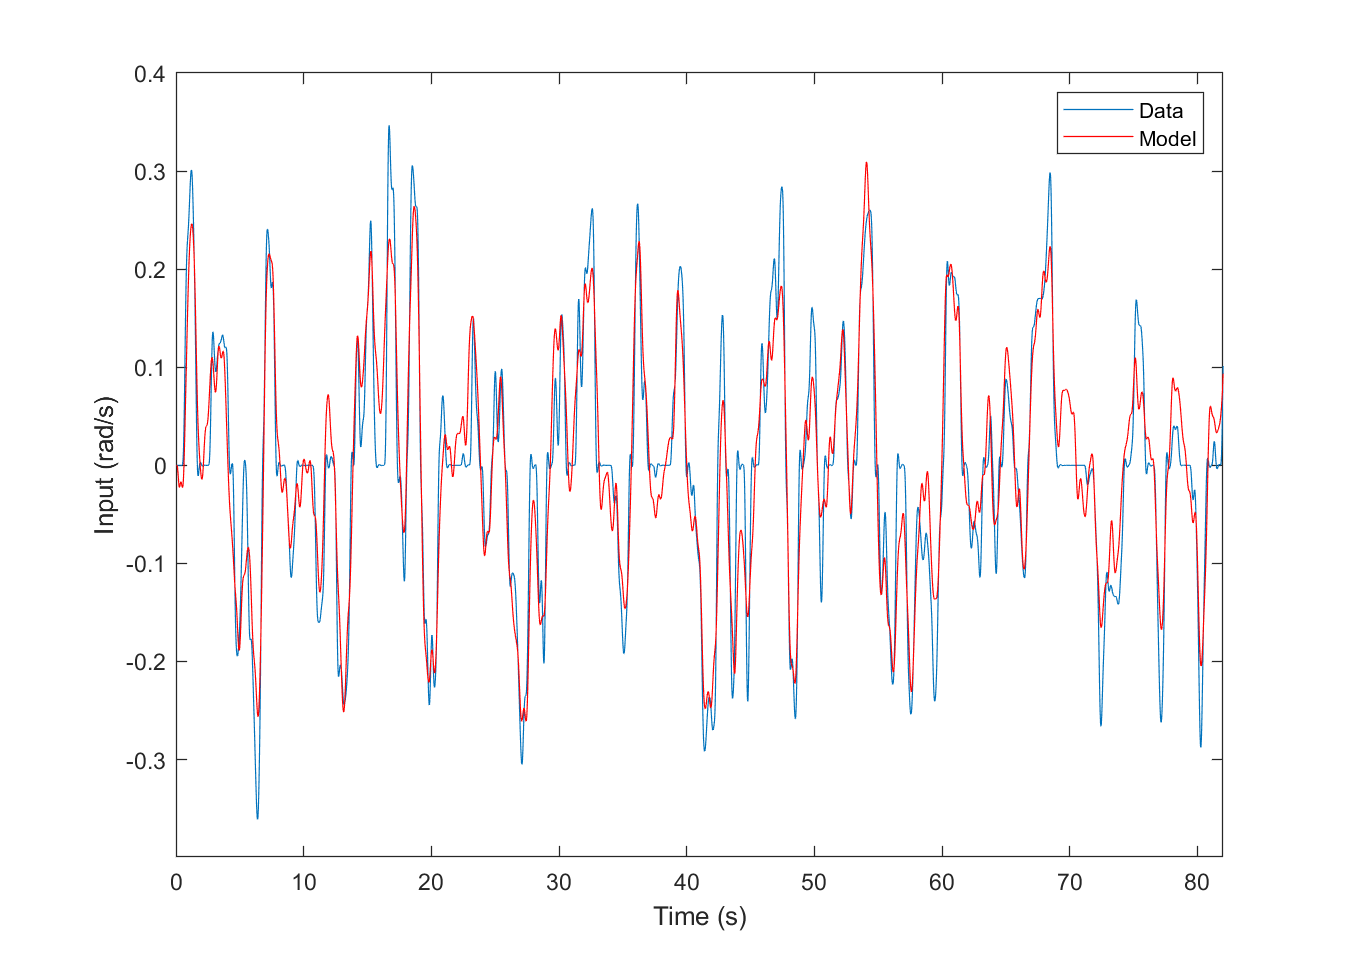
\includegraphics[width=0.8\textwidth]{figures/Modeling/model_output.png}
        \caption[Comparison between estimated transfer function model and experimental data]{Comparison between estimated transfer function model and experimental data.}
        \label{fig:comparison}
    \end{subfigure}
    \hfill
    \begin{subfigure}[b]{\textwidth}
        \centering
        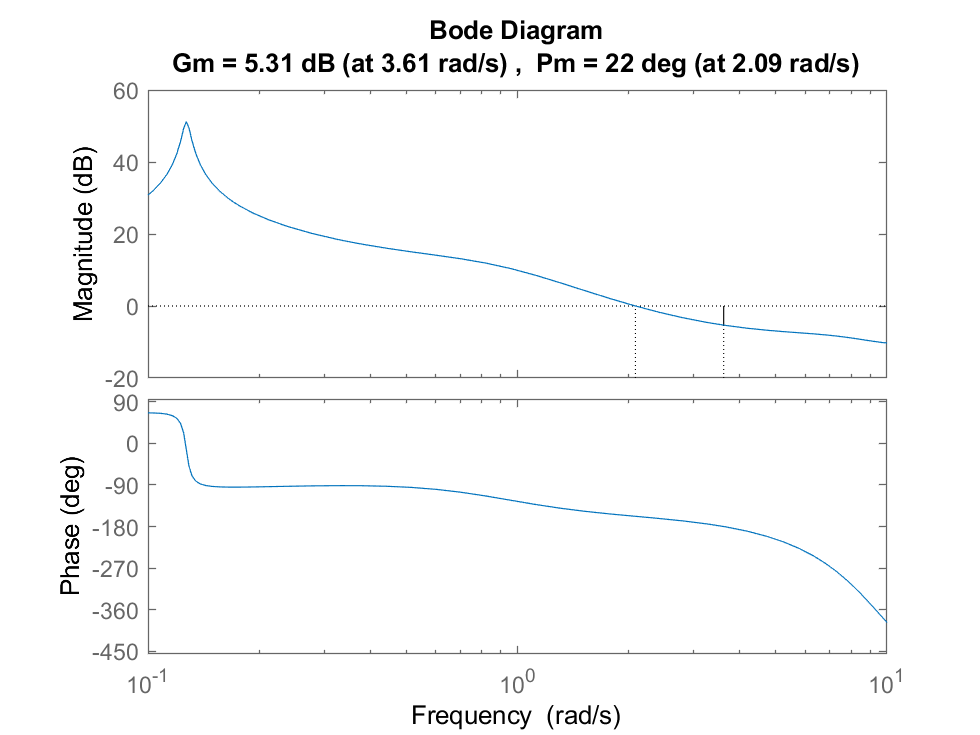
\includegraphics[width=0.8\textwidth]{figures/Modeling/YpYc_204.png}
        \caption[Combined pilot/vehicle open-loop bode diagram]{Combined pilot/vehicle open-loop bode diagram showing the standard crossover model characteristics.}
        \label{fig:bode}
    \end{subfigure}
    \caption[Example results from using the estimated pilot models from \textit{gettf1}]{Example results from using the estimated pilot models from \textit{gettf1}.}
    %    \label{fig:goodnessoffit}
\end{figure}

The VAF of the feedback group's models immediately jumps up after the first trial to an average of $\approx.75$, indicating a good fit.
The control groups VAF increases more slowly, to a value of approximately $\approx.68$.
An increased VAF indicates that the pilot is behaving in a more linear fashion, and these results suggest that the concurrent feedback is able to immediately assist participants to this end.
The RMSE between the simulated and actual data is similar between groups and trends slightly up during training.
Visual inspection of the experimental and simulated data also shows very good agreement, see Figure~\ref{fig:comparison}.

By combining these pilot models with the system dynamics the crossover frequency (Figure~\ref{fig:bode}) and gain and phase margins can be found.
The crossover model has long been used as the standard model for human control tasks, where the crossover frequency represents ``how hard'' the pilot is working~\citep{mcruer_dynamic_1957}.
The results of these parameters reflect what was found in the pitch RMSE performance analysis.
Subjects in the feedback group immediately show increased crossover frequency and decreased phase and gain margins.
These results are sustained during retention, and again show an immediate increase/decrease when the feedback is removed.

\begin{figure}
    \centering
    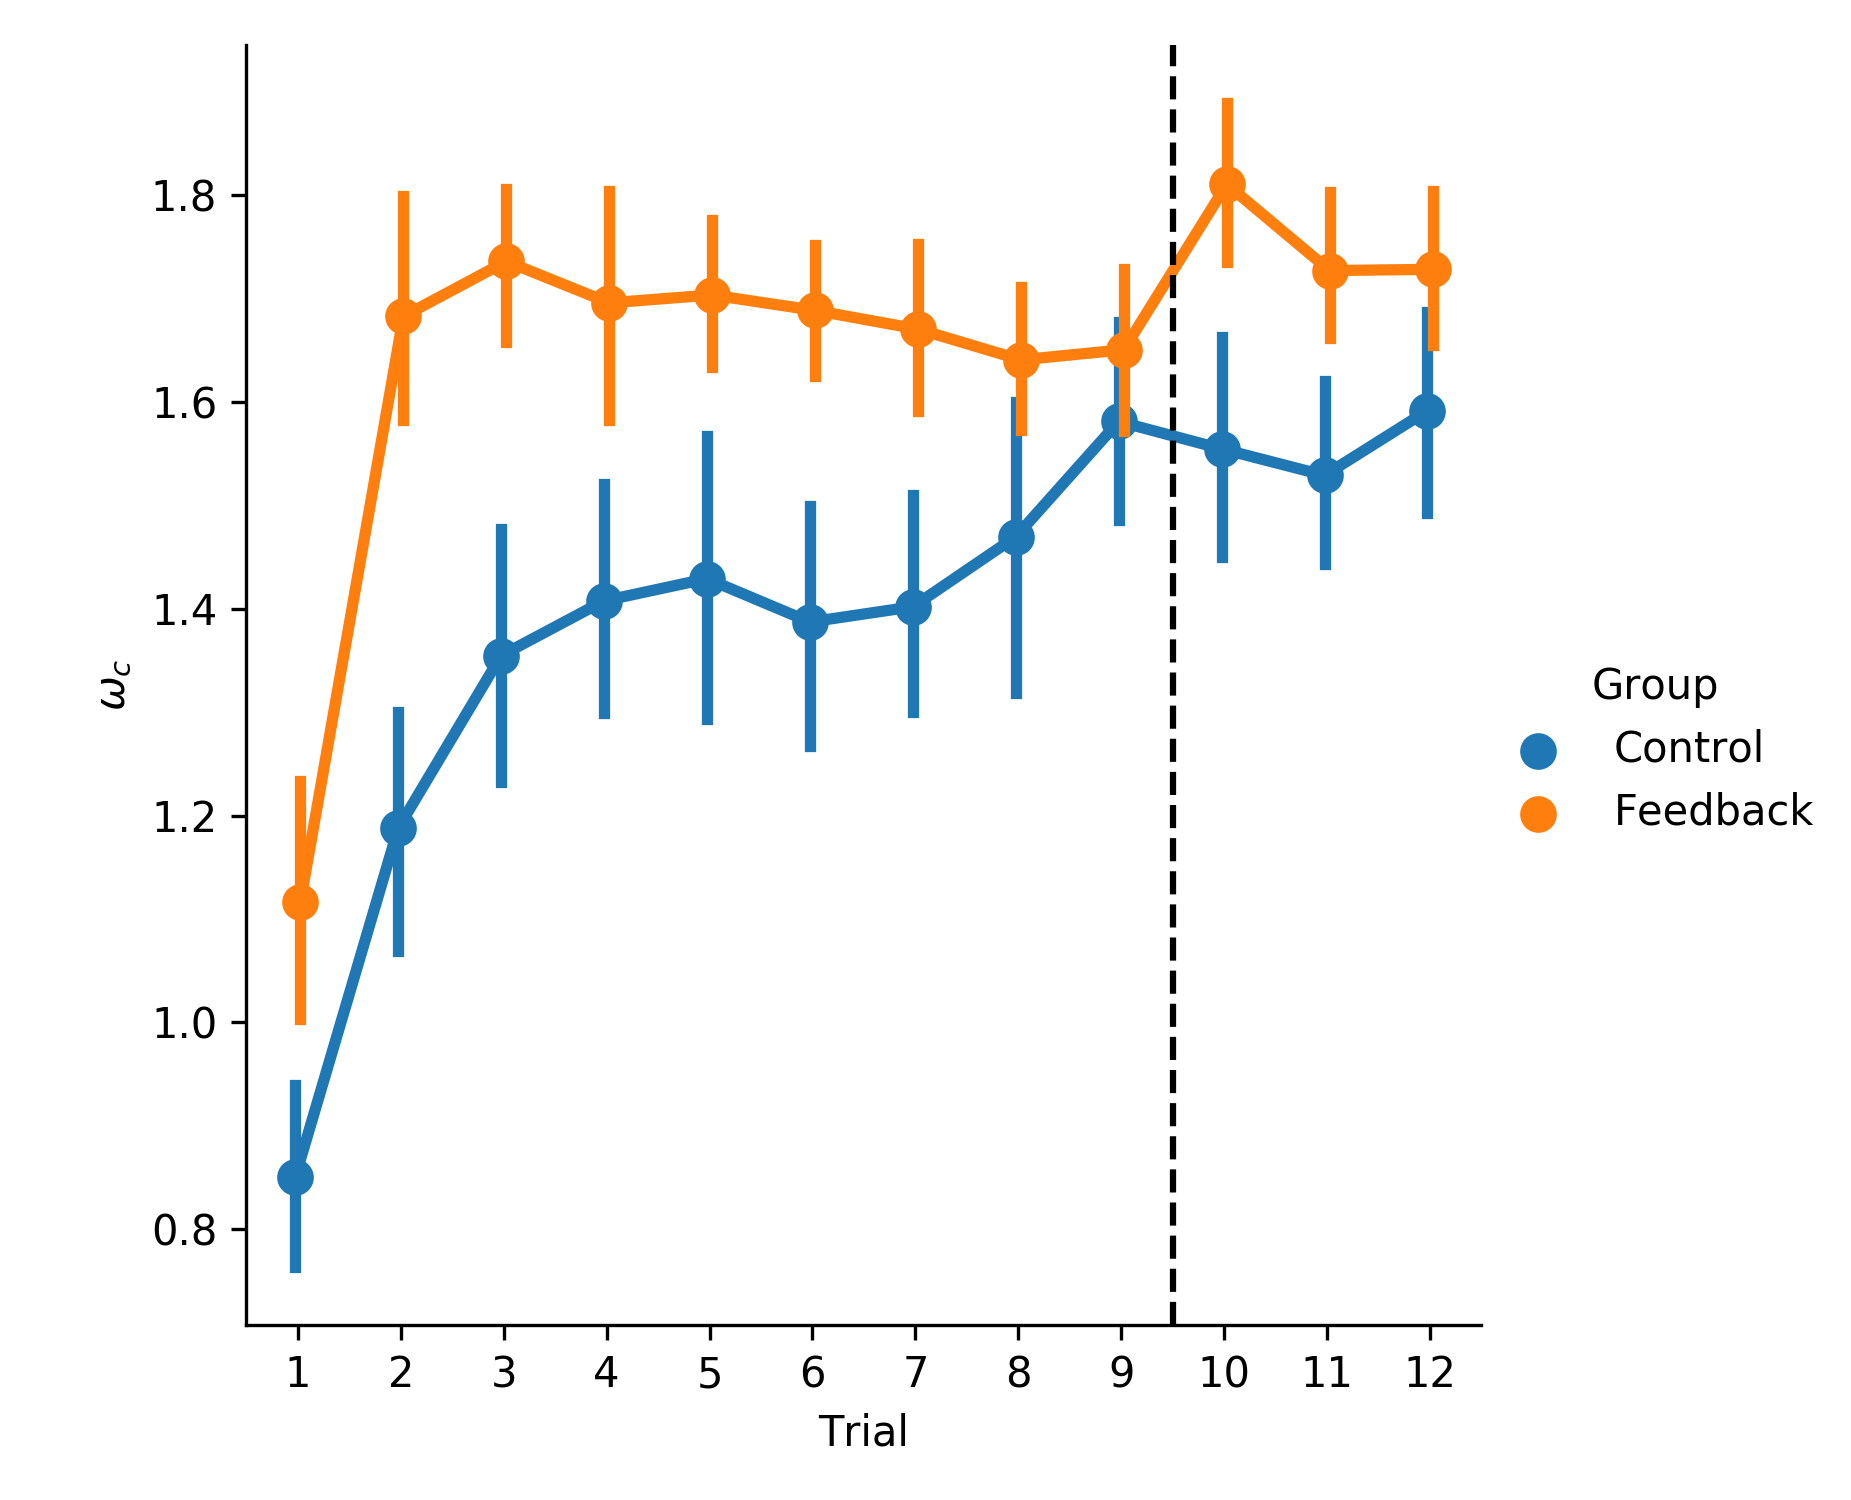
\includegraphics[width=0.8\linewidth]{figures/Modeling/wc_arx.png}
    \caption[Crossover frequency (ARX)]{Crossover frequency predicted by the ARX technique.}
    \label{fig:arx_crossover}
\end{figure}

Mixed models were used to calculate the significance of factors in our analysis due to the presence of performance outliers which were removed from the analysis.
The Satterthwaite method was used to calculate the adjusted degrees of freedom using the lmerTest package in R~\citep{RN53}.
When significant effects were observed, post hoc comparisons using the Tukey Honest Significance Difference (HSD) test were performed and considered significant at the $p < .05$ level, and the Satterthwaite method was again used to calculate the degrees of freedom.
Only 7 of the 1080 total trials (30 subjects with 36 trials per subject) were removed.
These trials were extreme performance outliers, and including these trials does not change the primary results of the study.

A three-factor (Group, Mode, and Trial) mixed model with two repeated measures (Mode and Trial) was run on the pitch crossover frequency.
There were significant main factors of group $(F(1, 28.00) = 4.9, p = 0.036)$, mode $(F(2, 55.62) = 17.1, p < .001)$, and trial $(F(11, 306.23) = 39.4, p < .001)$.
There were also significant interaction effects between group and trial $(F(11, 306.23) = 2.0, p = 0.025)$ and between mode and trial $(F(22, 610.08) = 2.8, p < .001)$.
Despite the presence of interaction effects that result from participants learning the task (as indicated by the trial factor), the main effects can still be interpreted.
A Tukey test showed that the participants in the groups differed significantly, with the participants in the feedback group outperforming those in the control group $(M = 1.25, 1.56,$ respectively, $SE = 0.10)$.
An additional Tukey test showed that the participants' crossover frequency between the modes differed significantly, with the largest crossover frequency in the P mode, followed by the PR mode, and finally the lowest in the PRA mode $(M = 1.53, 1.38, 1.31$ respectively, $SE = 0.07)$.
This same analysis was completed on the roll crossover frequency, with similar results.
There were significant main factors of group $(F(1, 27.82) = 8.2, p < 0.01)$, mode $(F(1, 25.49) = 23.2, p < 0.001)$, and trial $(F(11, 292.40) = 16.3, p < .001)$.
Tukey tests showed that the participants' crossover frequency between the groups and the modes each differed significantly, with the participants in the feedback group again outperforming those in the control group $(M = 0.55, 0.89,$ respectively, $SE = 0.08)$, and crossover frequency was best in the PR mode followed by the PRA mode $(M = 0.77, 0.67,$ respectively, $SE = 0.06)$.
A two-factor (Group and Trial) mixed model with one repeated measure (Trial) was run on the altitude crossover frequency.
There were significant main factors of group $(F(1, 27.92) = 4.4, p = 0.046)$ and trial $(F(11, 301.95) = 18.3, p < .001)$.
Tukey tests showed that the participants' crossover frequency between the groups differed significantly, with the participants in the feedback group again outperforming those in the control group $(M = 0.98, 1.29,$ respectively, $SE = 0.11)$, and the trial effect showing learning throughout the experiment for both groups.

\subsection{Structural Model}
\subsubsection{Value Identification Technique}
A brute force parameter search was used to identify the value of the remaining parameters.
Each combination of the parameters $K_e, \tau_0, K, a$, and $\omega_{NM}$ were enumerated over and simulated in Simulink using the same flight model and disturbance profiles as the participants experienced in the experiment.
The resulting 102,600 simulations were compared to each trial to identify the set of parameter values resulting in the smallest VAF.

Once this initial global best fit was identified, the parameters were further tuned in MATLAB using ``fmincon'' to find the minimum of the constrained nonlinear multivariable function.
The constraints for the solver were the bounds of the global brute force search, though, in general, the optimizer did not result in large parameter changes from the initial values.

\begin{align}
\nonumber    K_e         & = [1, 2, 3, \ldots, 30]         \\
\nonumber    \tau_0      & = [.20, .25, .30] \mbox{s}             \\
\nonumber    K           & = [1.0, 1.5, 2.0, \ldots, 10.0] \\
\nonumber    a           & = [.0, .25, .50, \ldots, 3.0]   \\
\nonumber    \omega_{NM} & = [7, 8, 9, 10, 11, 12] \mbox{rad/s}   \\
\nonumber    \zeta_{NM}  & = [0.7] \mbox{rad/s}
\end{align}

% Structural Model Parameter Identification Technique

% 	Run (Parallel)ModelGenerator.m in MATLAB to generate many model outputs.
% 	Run ExperimentMatcher.py in Python to identify the global optimum best initial set of parameters.
% 	Run ModelOptimizer.m in MATLAB to iterate on the initial guess to identify an optimal set of parameters.
% 	Run ModelAnalysis.r in R to generate the statistics.
% 	Run OptimalModelPlots.py in Python to make the plots.

% Ke
% Type III Analysis of Variance Table with Satterthwaite's method
%       Sum Sq Mean Sq NumDF DenDF F value    Pr(>F)
% group  113.8  113.80     1    27  7.2654   0.01195 *
% trial 1493.7  135.79    11   308  8.6693 2.201e-13 ***
% ---
% Signif. codes:  0 ‘***’ 0.001 ‘**’ 0.01 ‘*’ 0.05 ‘.’ 0.1 ‘ ’ 1

% tdel
% Type III Analysis of Variance Table with Satterthwaite's method
%         Sum Sq   Mean Sq NumDF DenDF F value Pr(>F)
% group 0.000176 0.0001760     1    27  0.0171 0.8968
% trial 0.068712 0.0062466    11   308  0.6081 0.8217

% Ypf
% Type III Analysis of Variance Table with Satterthwaite's method
%       Sum Sq Mean Sq NumDF DenDF F value Pr(>F)
% group 12.032  12.032     1    27  1.6509 0.2097
% trial 82.819   7.529    11   308  1.0331 0.4168

% a
% Type III Analysis of Variance Table with Satterthwaite's method
%        Sum Sq Mean Sq NumDF DenDF F value   Pr(>F)
% group  0.0031 0.00314     1    27  0.0068 0.934953
% trial 13.6429 1.24026    11   308  2.6798 0.002657 **
% ---
% Signif. codes:  0 ‘***’ 0.001 ‘**’ 0.01 ‘*’ 0.05 ‘.’ 0.1 ‘ ’ 1

% Wnm
% Type III Analysis of Variance Table with Satterthwaite's method
%        Sum Sq Mean Sq NumDF DenDF F value Pr(>F)
% group   0.477  0.4768     1    27  0.0487 0.8270
% trial 130.831 11.8937    11   308  1.2141 0.2764

% Zetanm
% Type III Analysis of Variance Table with Satterthwaite's method
%          Sum Sq    Mean Sq NumDF DenDF F value  Pr(>F)
% group 0.0000331 0.00003309     1    27  0.1937 0.66338
% trial 0.0035074 0.00031886    11   308  1.8665 0.04314 *
% ---
% Signif. codes:  0 ‘***’ 0.001 ‘**’ 0.01 ‘*’ 0.05 ‘.’ 0.1 ‘ ’ 1

% All variables can be treated as constants with the exception of  K_e, which changes with both Trial and Group.
% tdel	Ypf	a	Wnm	Zetanm
% 0.238±0.006	5.927±0.163	1.301±0.041	7.768±0.185	0.707±0.001

% Model K_e as Exponential Fit: K_e=A*e^(-B*Trial)+C

% 	A	B	C
% Control	-7.34466243	0.37349137	12.40429001
% Feedback	-67.32338104	1.99463577	17.40238421

\begin{figure}[t]
    \centering
    \centering
    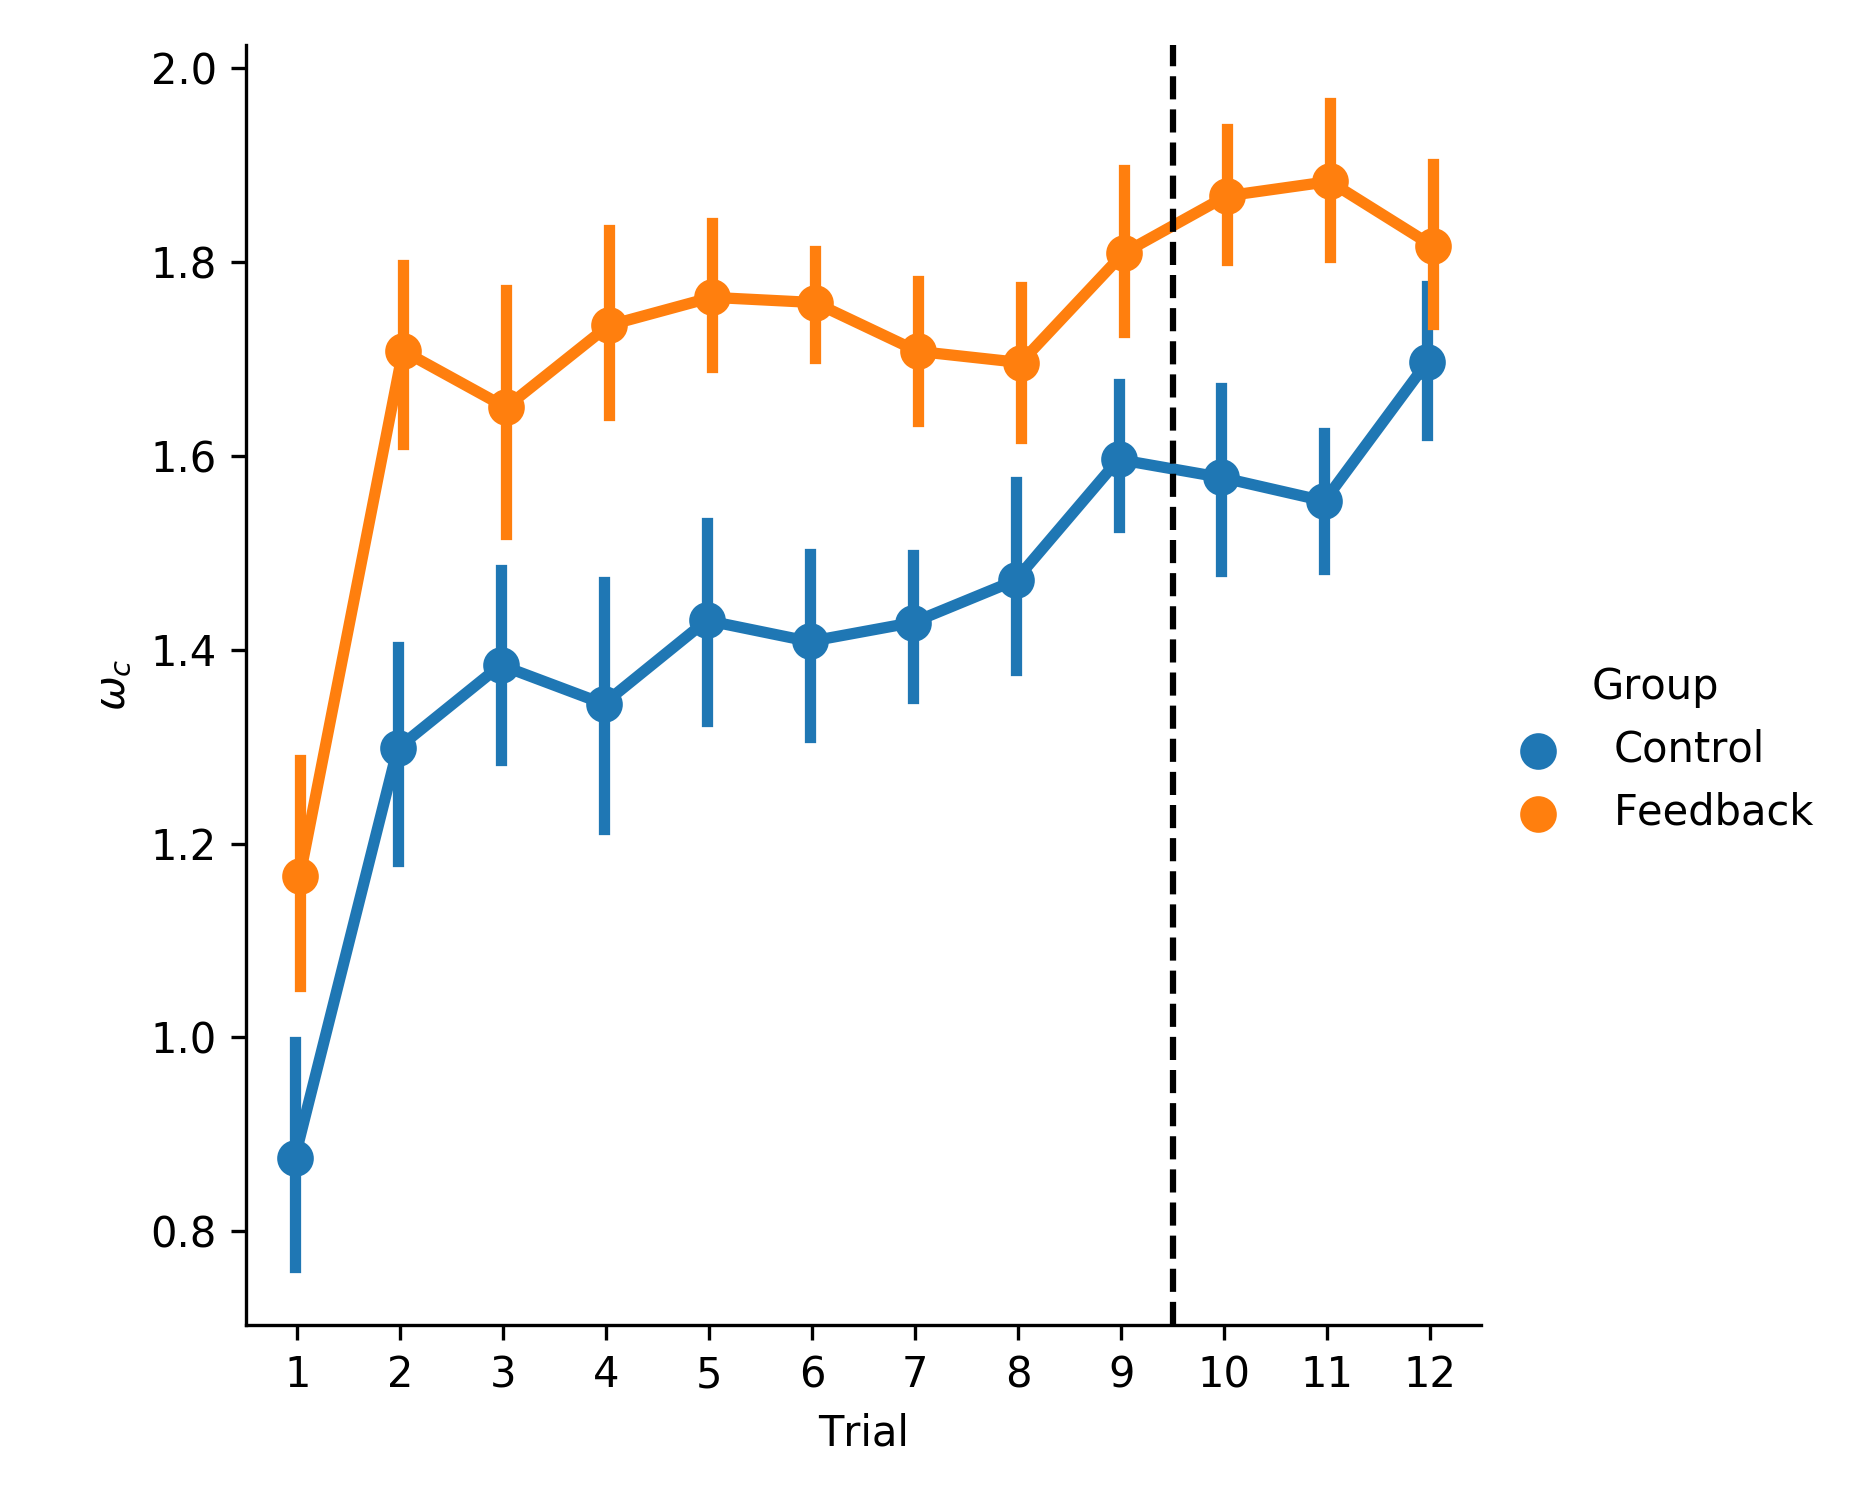
\includegraphics[width=0.8\linewidth]{figures/Modeling/wc_group.png}
    \label{fig:sm_crossover}
    \caption[Crossover frequency (Structural Model)]{Crossover frequency predicted by the Structural Model parameter identification.}
\end{figure}

\begin{figure}[t]
    \centering
    \centering
    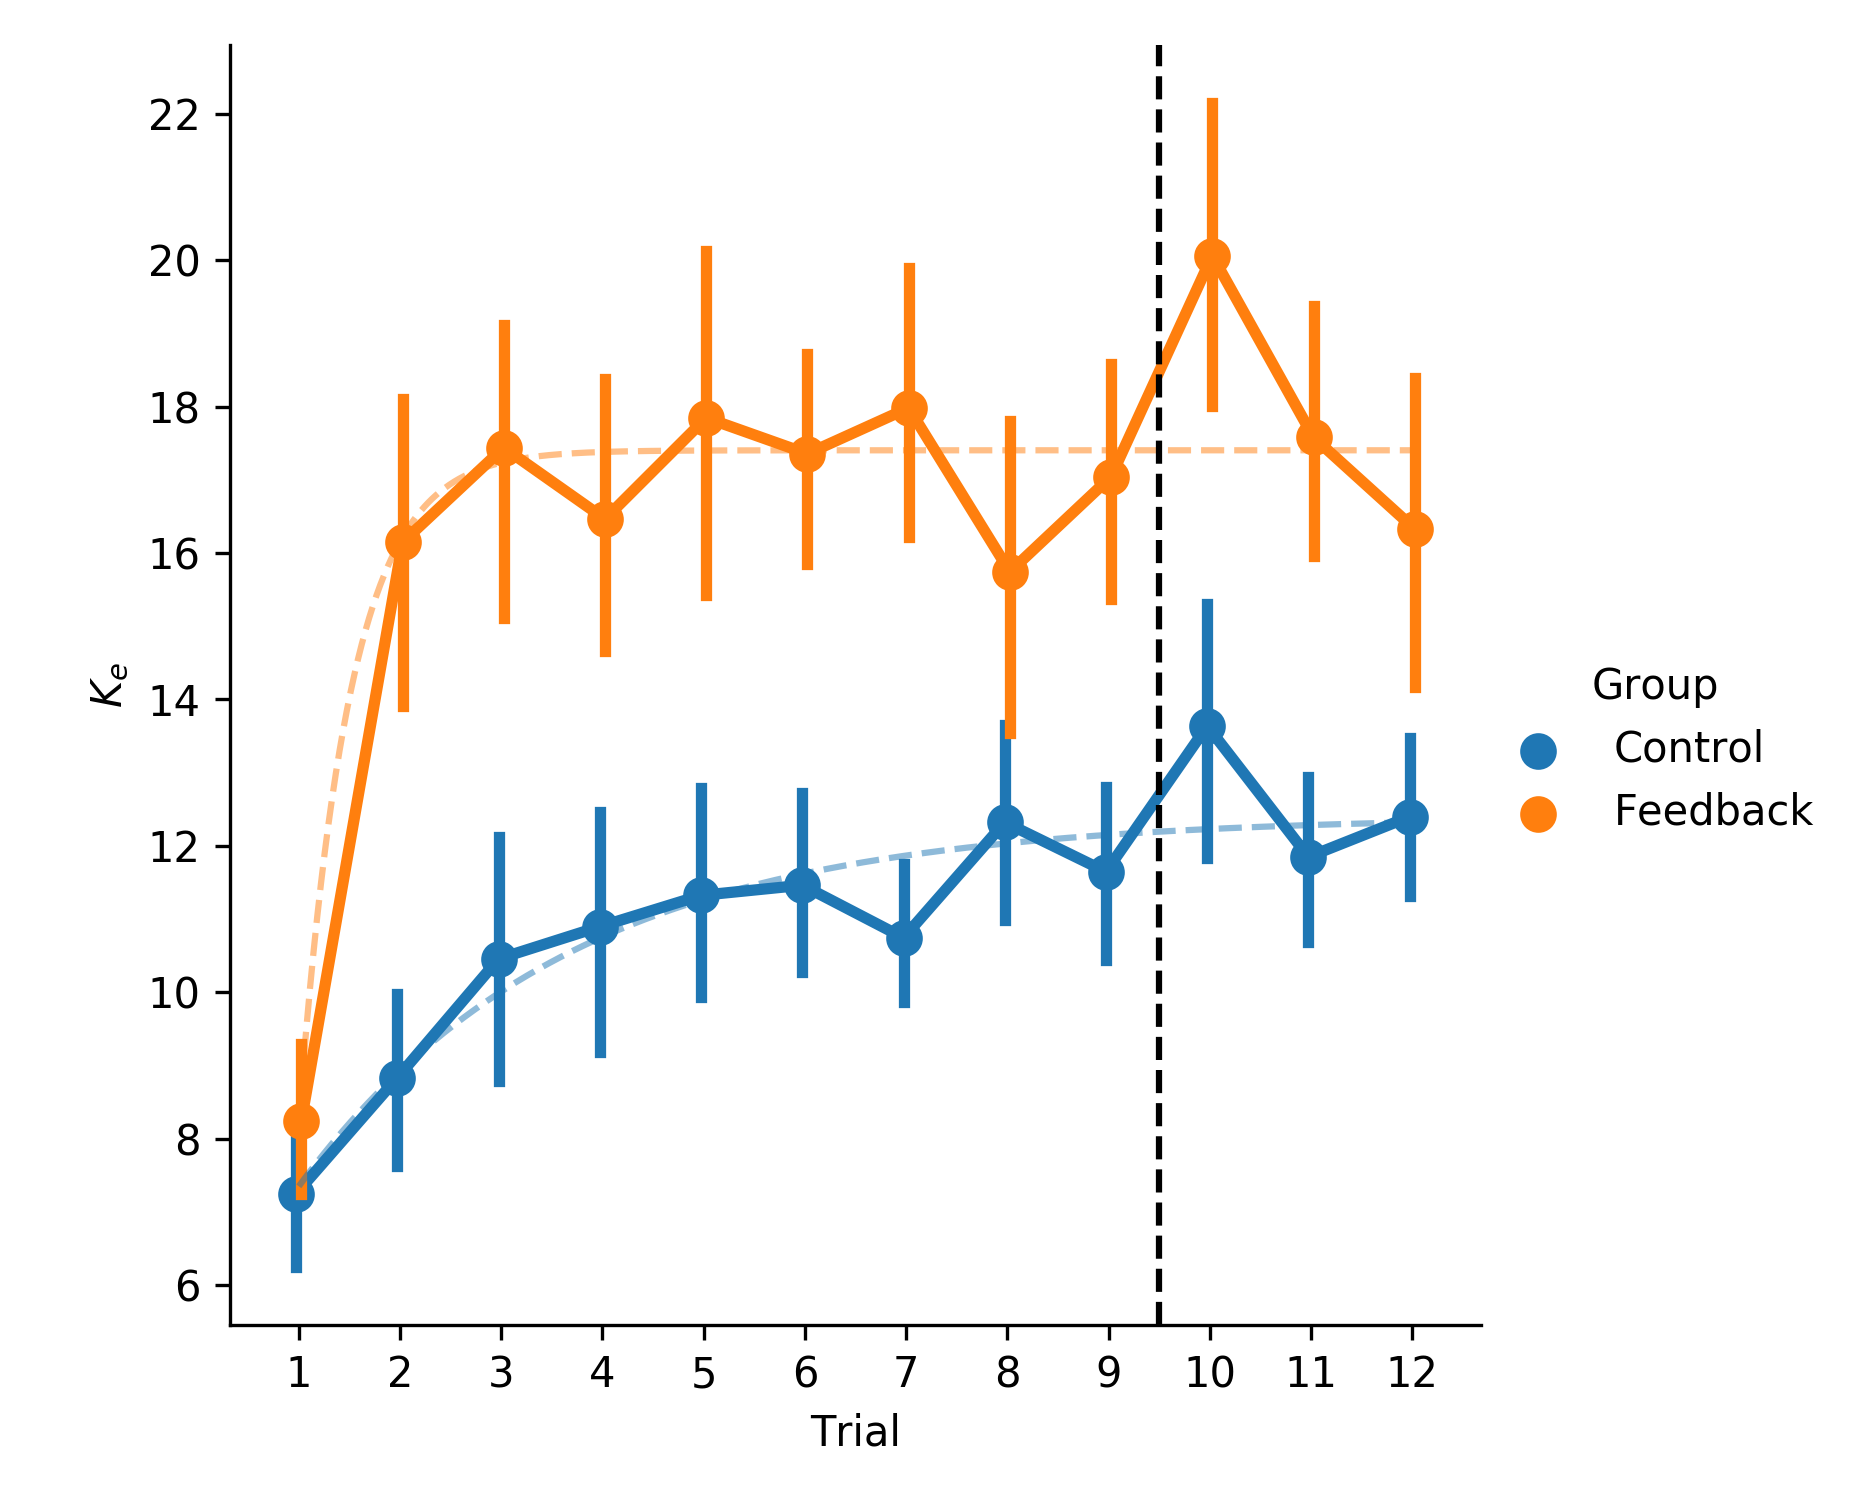
\includegraphics[width=0.8\linewidth]{figures/Modeling/ke_group.png}
    \label{fig:ke_group}
    \caption[$K_e$ is greater for subjects exposed to feedback]{$K_e$ is greater for subjects exposed to feedback.}
\end{figure}

\section{Extending the Structural Model}

\begin{figure}[t]
    \centering
    \centering
    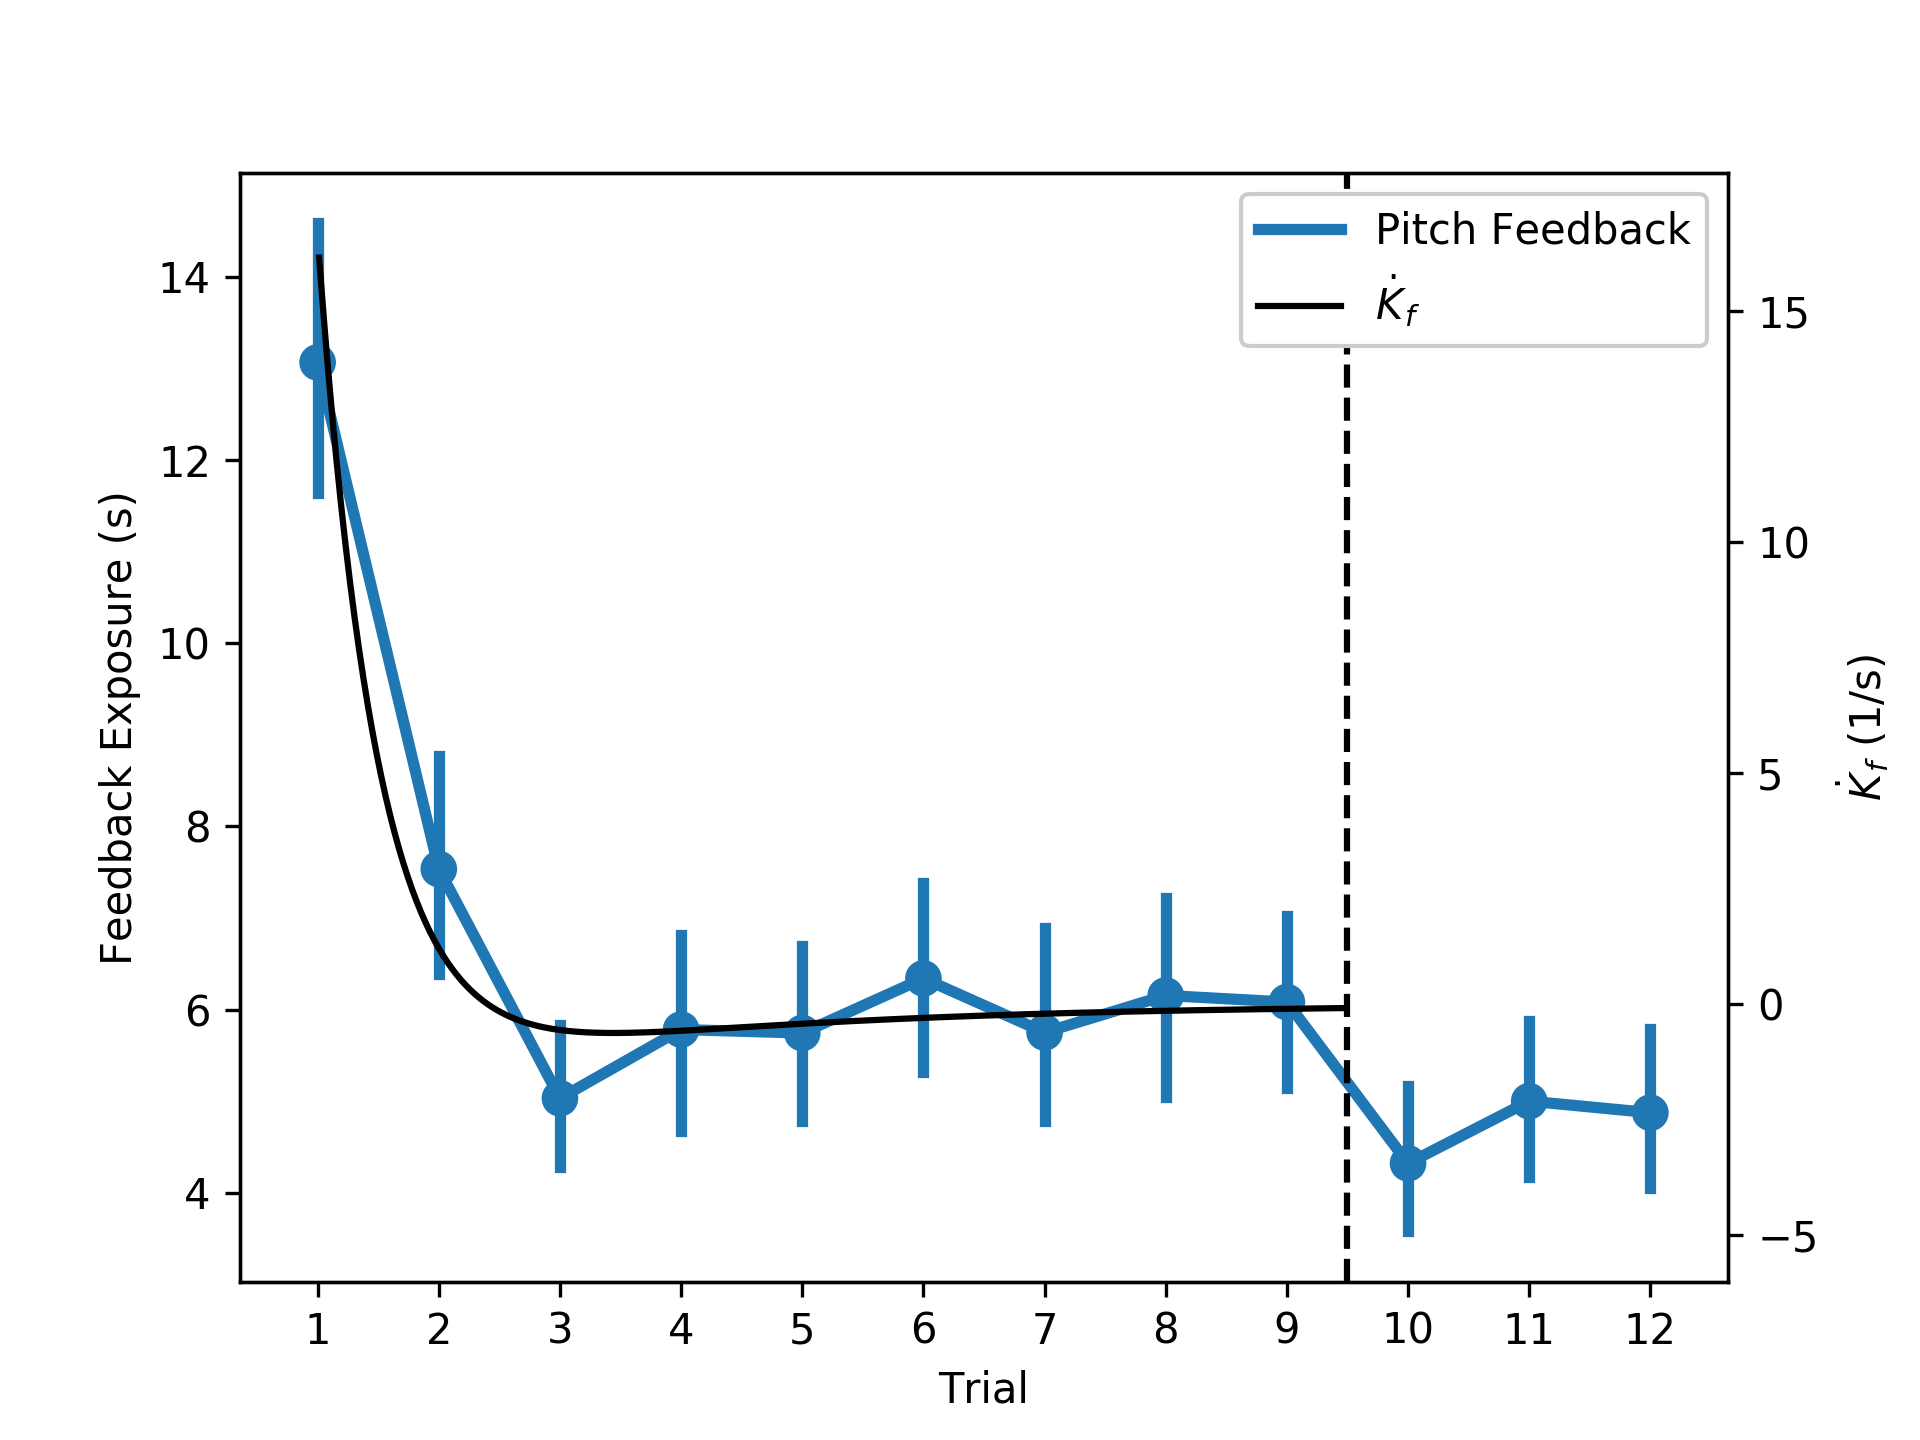
\includegraphics[width=0.8\linewidth]{figures/Modeling/f_v_kfd.png}
    \label{fig:feedback_kfd}
    \caption[Feedback exposure correlates with $\dot{K_f}$]{Feedback exposure correlates with $\dot{K_f}$, which confirms that the accumulation of exposure to feedback drives $K_f$.}
\end{figure}

\section{Discussion}
% \begin{figure*}
%     \centering
%     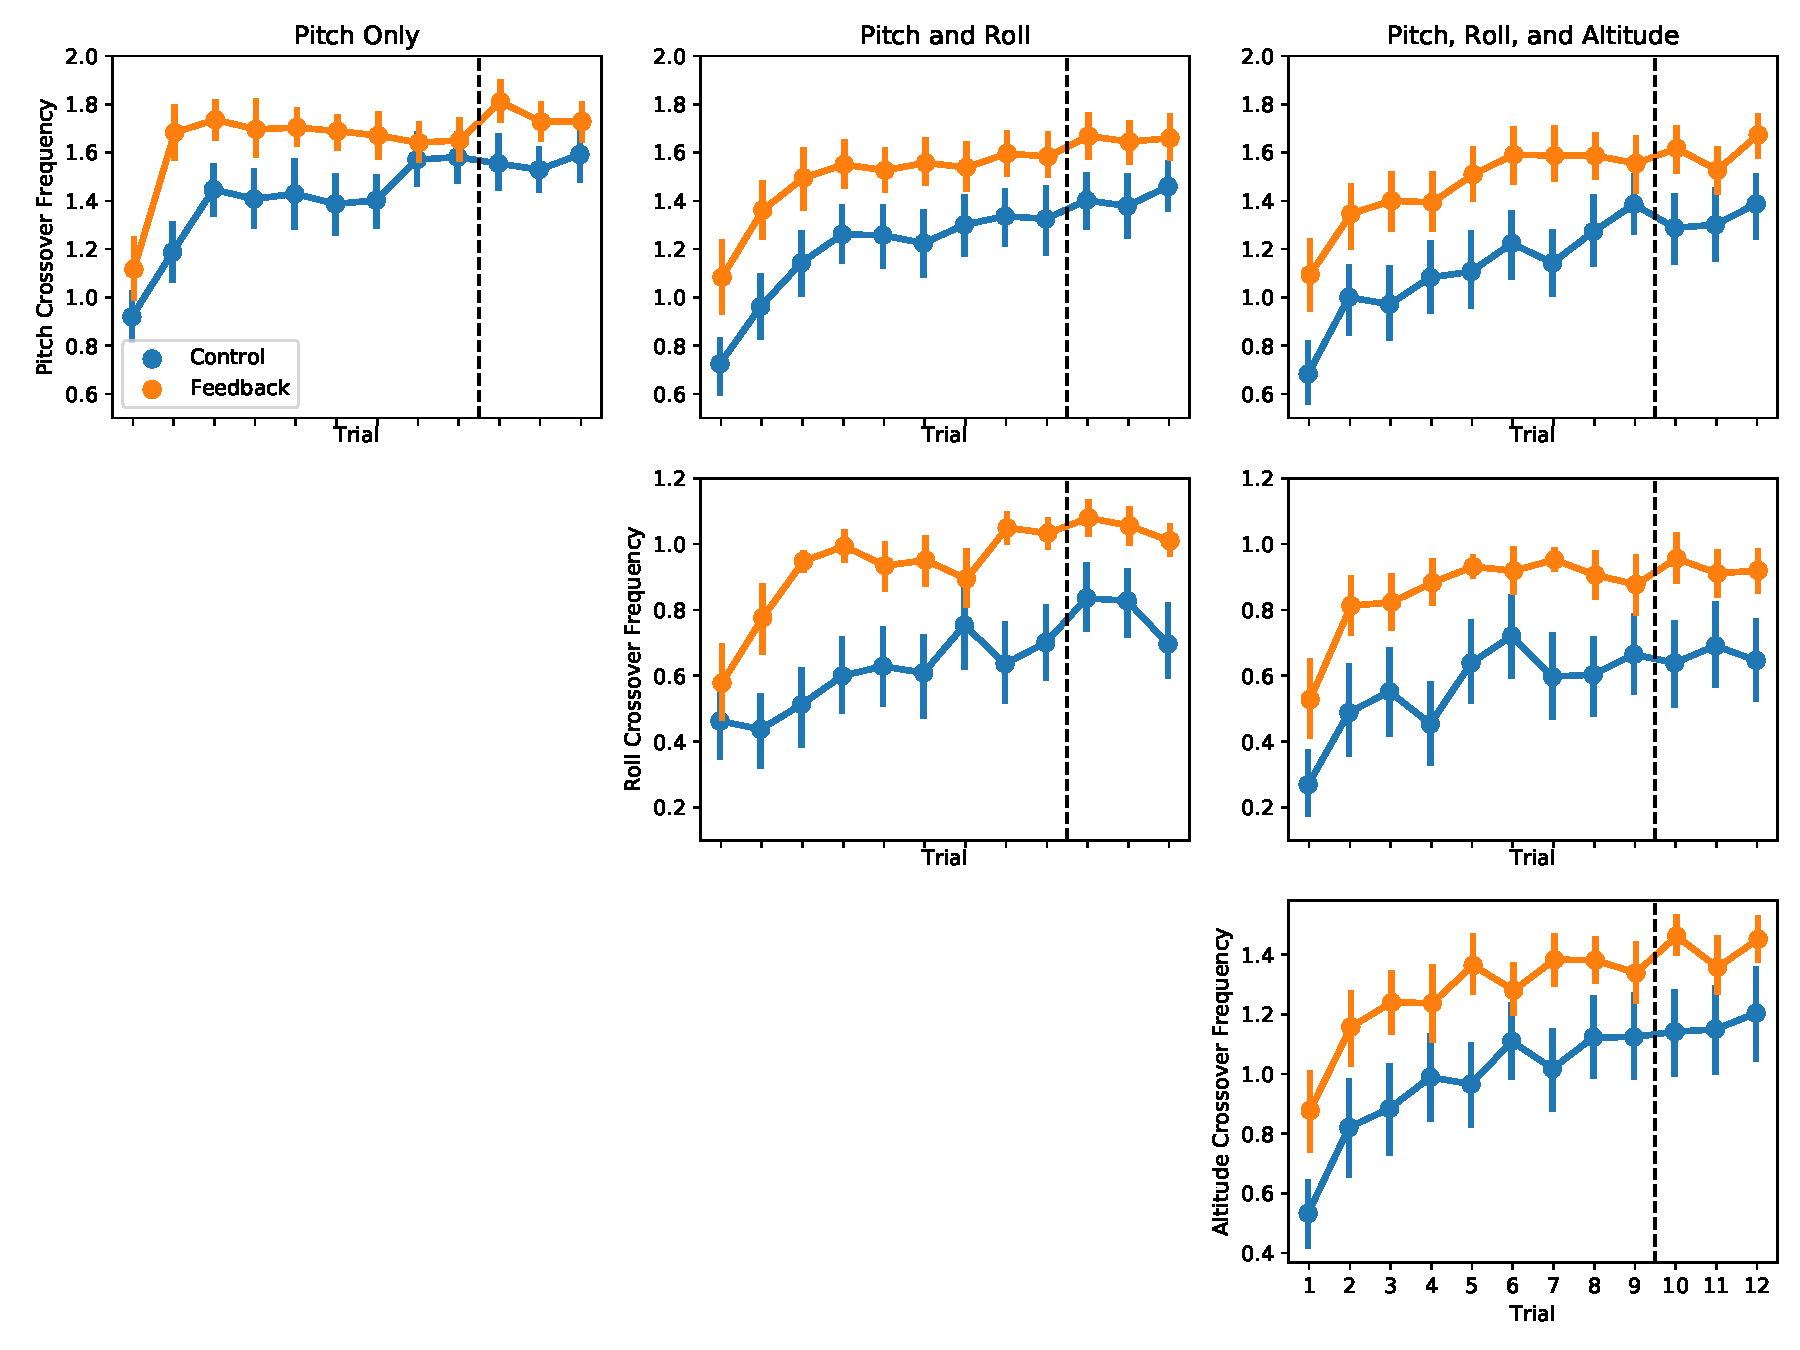
\includegraphics[width=6in]{figures/Modeling/crossover_measures.pdf}
%     \caption{The crossover frequency of the estimated pilot/vehicle open-loop transfer functions for each group, trial, and control task.
%         The dashed line indicates where the feedback was removed from participants in the feedback group.
%         Error bars are the standard error of the mean.}
%     \label{figure:crossover_frequency_all}
% \end{figure*}

A time-domain autoregressive exogenous (ARX) identification technique was used to estimate pilot transfer functions and the estimated pilot/vehicle open-loop transfer functions were evaluated to determine the evolution of the crossover frequency for each control loop throughout training.
The Hess Structural Model of the pilot was also investigated, which ``describe the underlying structure which contributes to human pilot dynamics.''
The Structural Model is of interest for interpreting the effects of concurrent feedback as it incorporates multiple sensory channels and models of visual acuity and the time-varying human pilot.
Results indicate that participants in the feedback group had a significantly lower root-mean-square error and higher crossover frequency than those in the control group, indicating better performance.
The ARX identification technique provided a consistently high variance accounted for (VAF), indicating that it can identify transfer functions representing a variety of operators at various levels of training.
These results are more pronounced for modes with increased functional complexity and persisted in retention testing when the feedback was removed, indicating that participants were not reliant on the feedback.

\chapter{Conclusion}
\label{chap:conclusion}

\textbf{\color{red} This chapter does not yet exist.}

\section{Research Questions}

In Chapter~\ref{sec:intro_questions}, we listed seven research questions that we aimed to answer by this research.
Here we summarize our answers to these questions.

\section{Future Work}



% note that the 'plainnat' style does not allow URL's in the bibtex entry
%
% some ideas here:
% http://bib2web.djvuzone.org/bibtex.html
%

% reset the page style
%\pagestyle{plain}


% To enable this it will need to be added to toc so it's not in a chapter
\pagestyle{plain}

\ssp
\bibliography{dissertation}

% the appendix:
% there are several sections, that don't really fit into the main chapters
%
\part*{\addcontentsline{toc}{part}{Appendices}Appendices}
\appendix

% reset page style to fancy
%\pagestyle{fancyplain}

\chapter{Trade Analysis Tables} \label{appendix:trade-tables}

\begin{figure}[b!]
    \begin{center}
        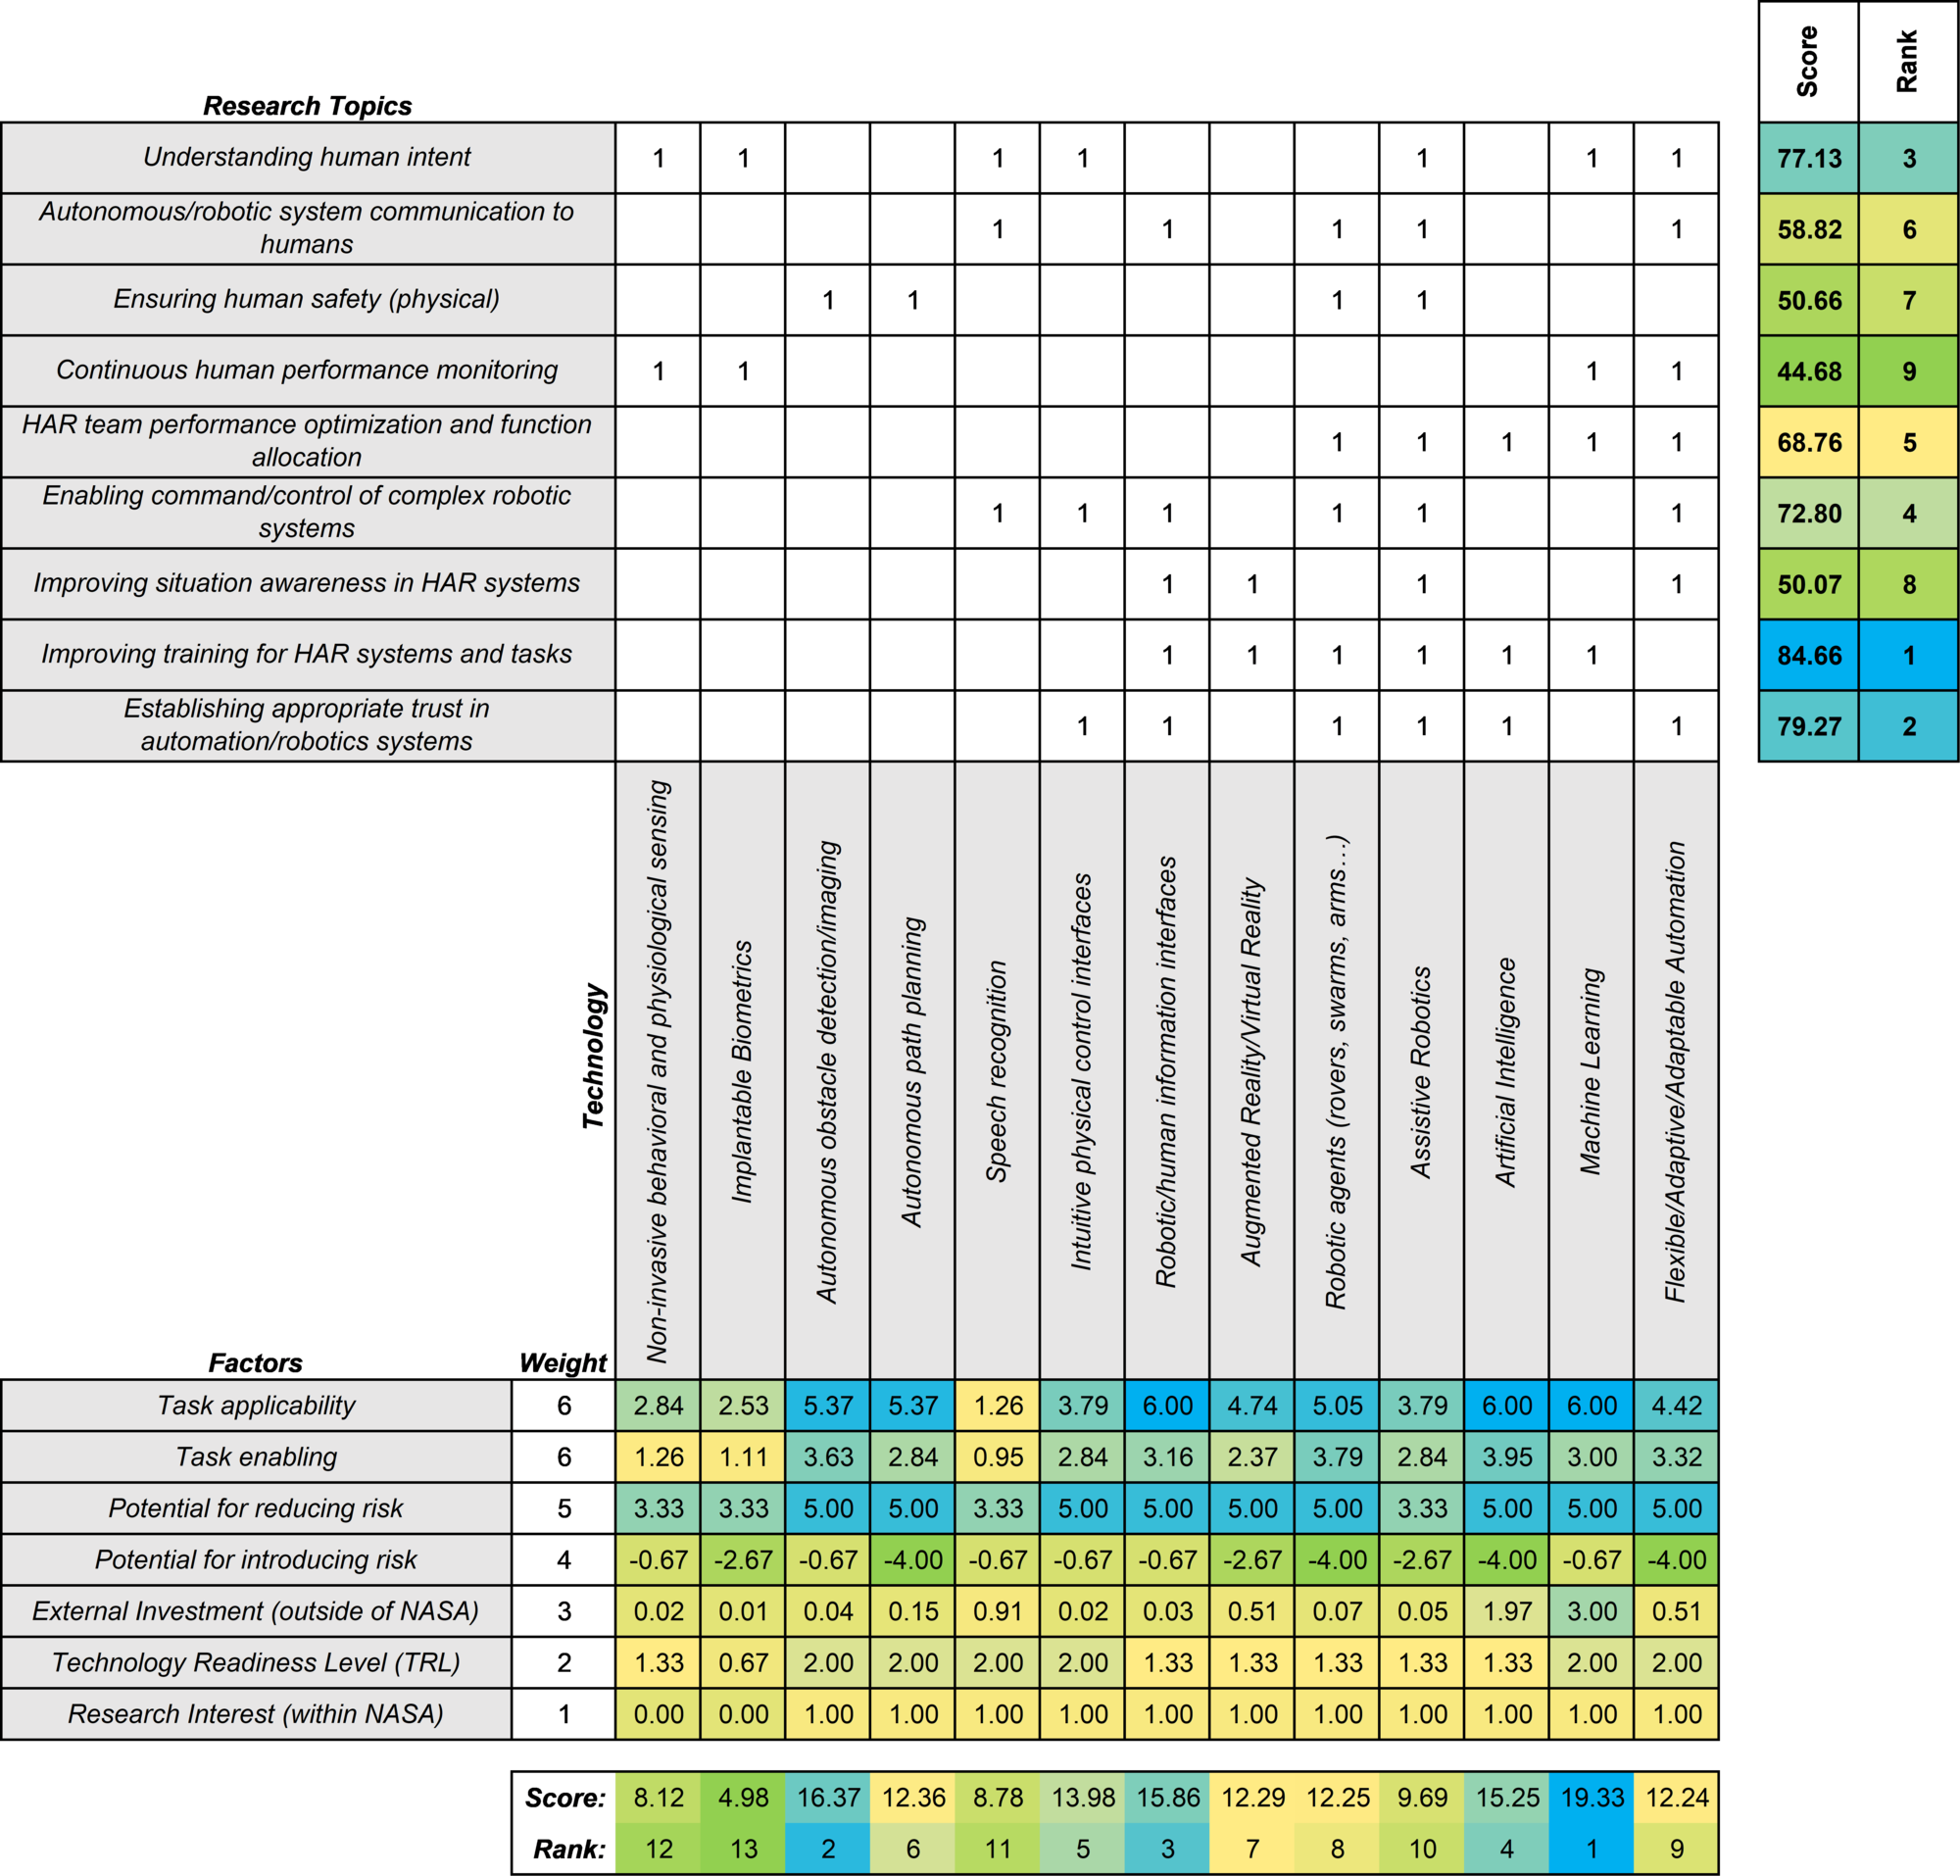
\includegraphics[width=0.8\linewidth]{figures/TradeStudy/figurea1.png}
        \caption[Top-level trade table]{Top-level trade table with final research topic scores (top right), final technology scores based on factors (bottom) and weighted factor-level scores for each technology.}
        % \label{figure:}
    \end{center}
\end{figure}

\begin{figure}[b!]
    \begin{center}
        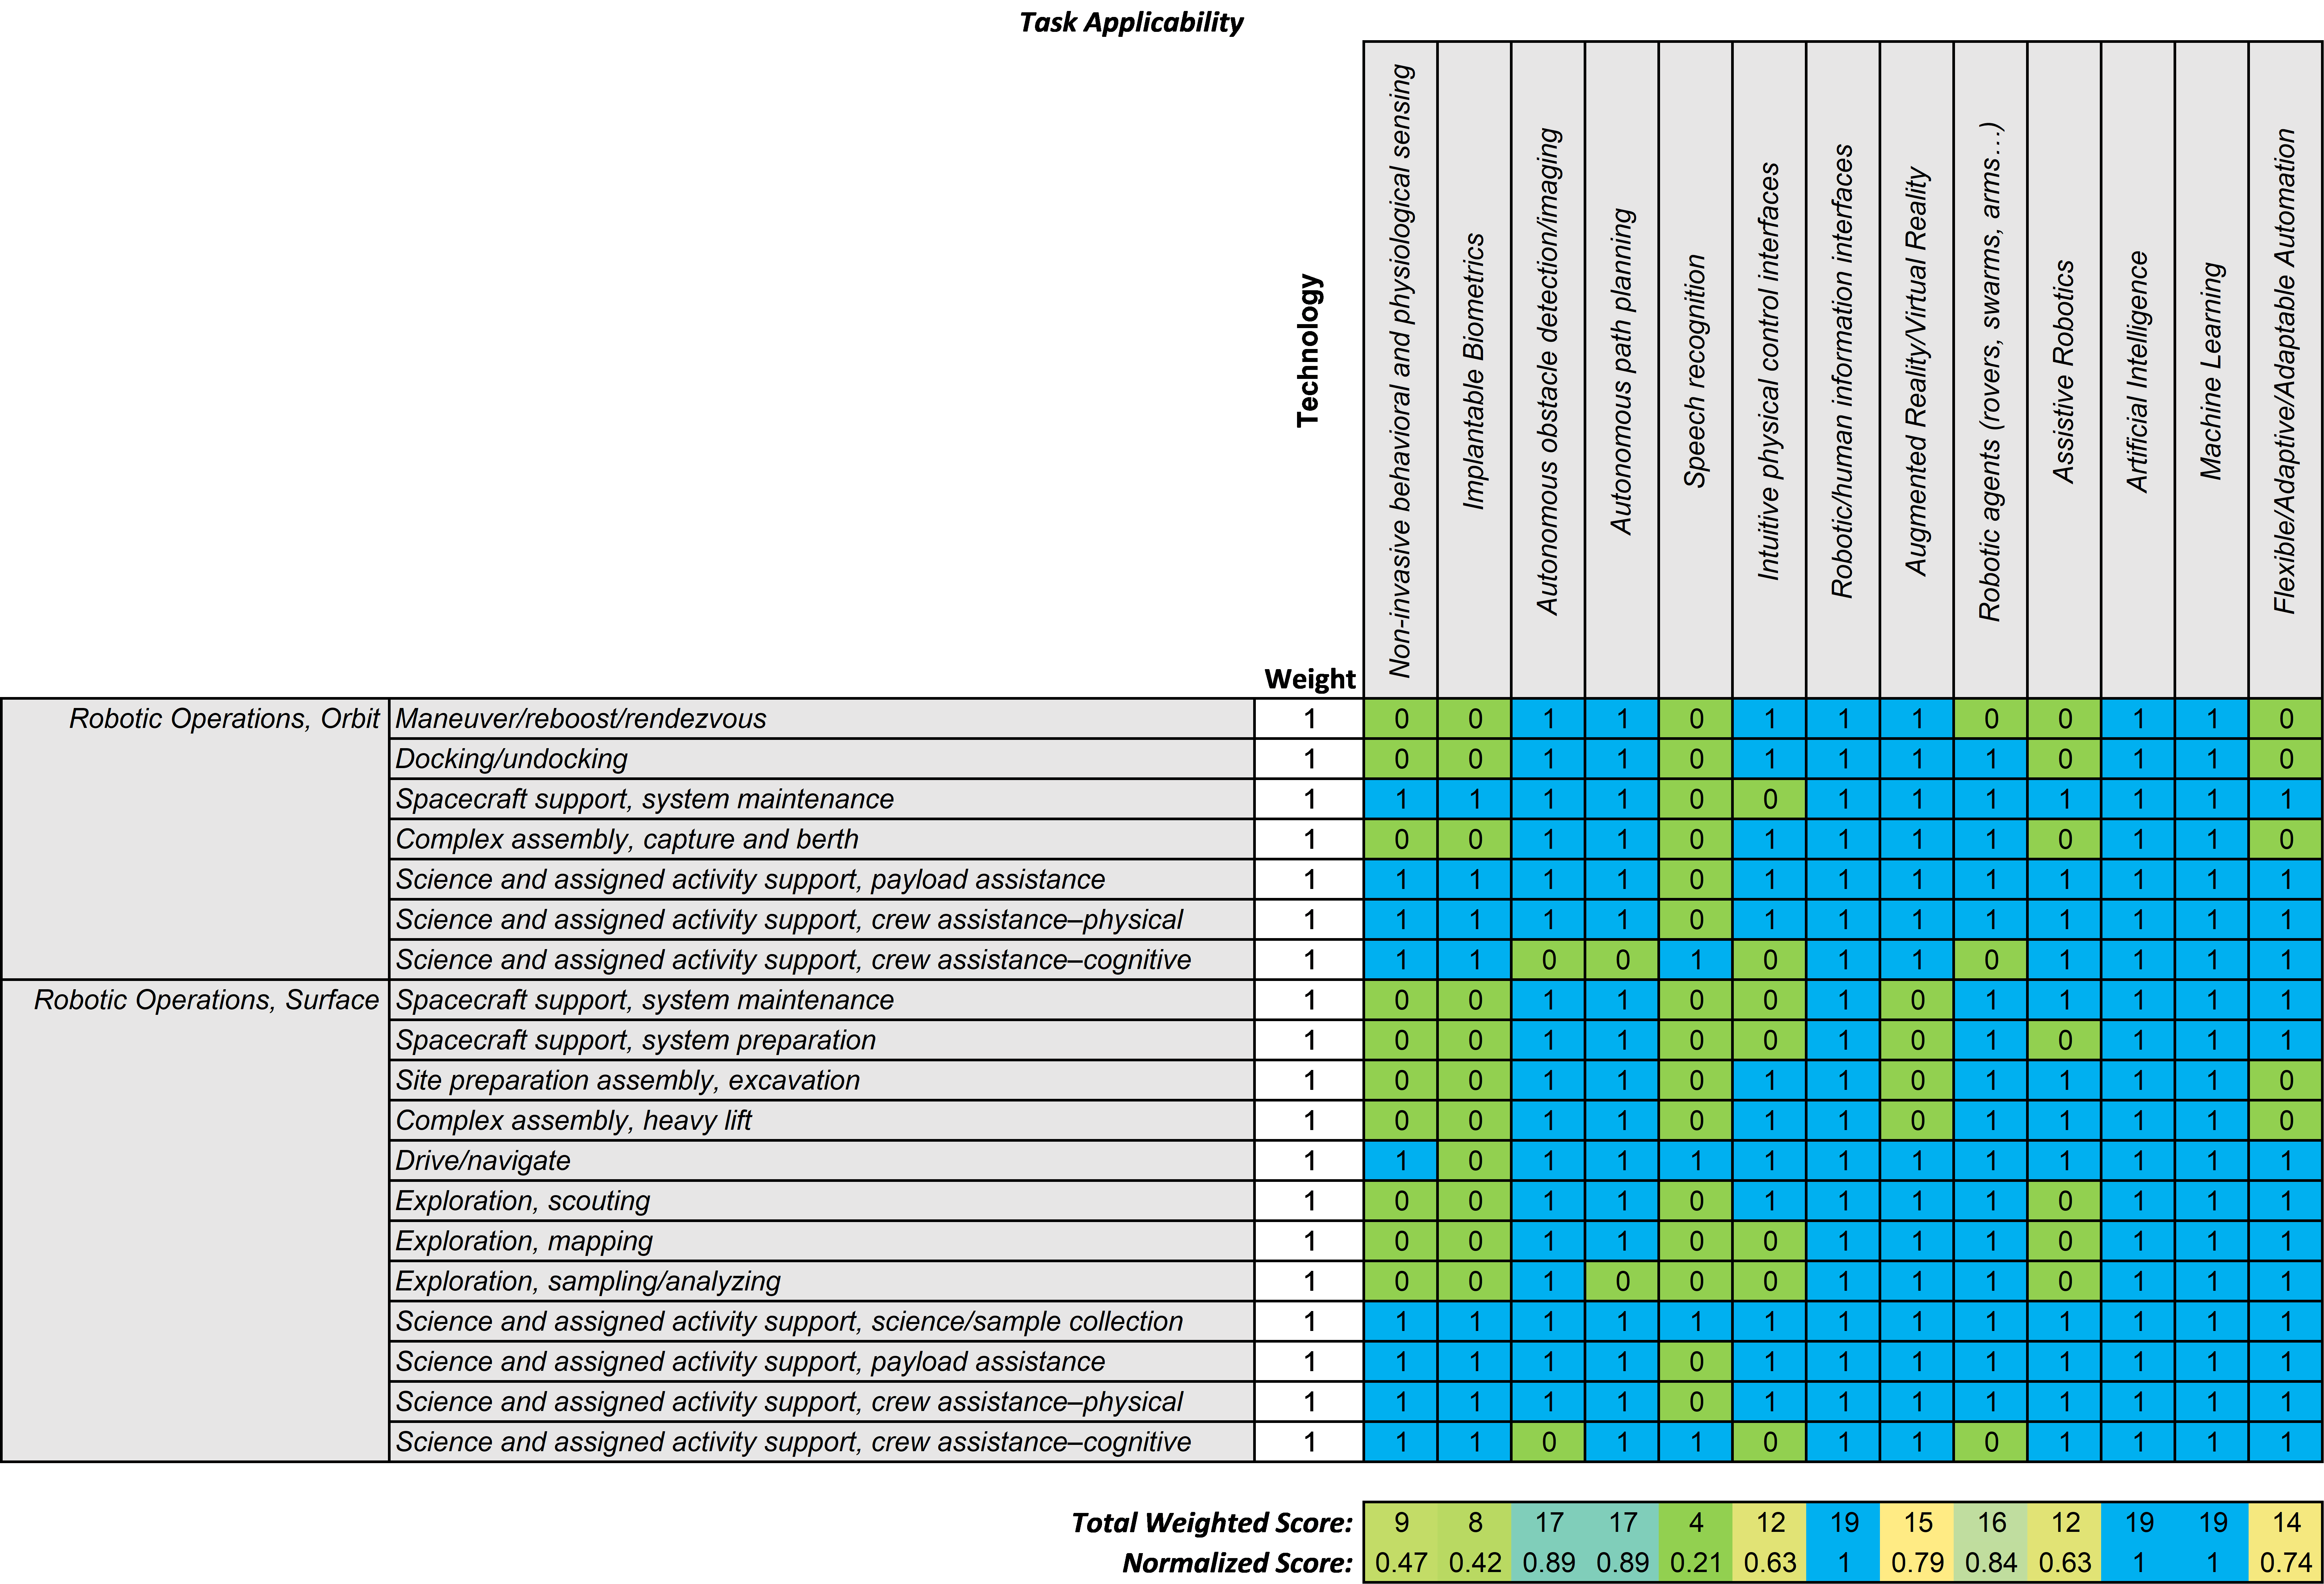
\includegraphics[width=0.8\linewidth]{figures/TradeStudy/figurea2.png}
        \caption[Technology to Task Applicability factor-level trade table]{Technology to Task Applicability factor-level trade table.}
        % \label{figure:}
    \end{center}
\end{figure}

\begin{figure}[b!]
    \begin{center}
        \includegraphics[width=0.8\linewidth]{figures/TradeStudy/figurea3.png}
        \caption[Technology to Task Enabling factor-level trade table]{Technology to Task Enabling factor-level trade table.}
        % \label{figure:}
    \end{center}
\end{figure}

\begin{figure}[b!]
    \begin{center}
        \includegraphics[width=0.8\linewidth]{figures/TradeStudy/figurea4.png}
        \caption[Technology to Risk Reduced factor-level trade table]{Technology to Risk Reduced factor-level trade table.}
        % \label{figure:}
    \end{center}
\end{figure}

\begin{figure}[b!]
    \begin{center}
        \includegraphics[width=0.8\linewidth]{figures/TradeStudy/figurea5.png}
        \caption[Technology to Risk Introduced factor-level trade table]{Technology to Risk Introduced factor-level trade table.}
        % \label{figure:}
    \end{center}
\end{figure}

\begin{figure}[b!]
    \begin{center}
        \includegraphics[width=0.8\linewidth]{figures/TradeStudy/figurea6.png}
        \caption[Technology to Research Interest (outside NASA) factor-level trade table]{Technology to Research Interest (outside NASA) factor-level trade table.}
        % \label{figure:}
    \end{center}
\end{figure}

\begin{figure}[b!]
    \begin{center}
        \includegraphics[width=0.8\linewidth]{figures/TradeStudy/figurea7.png}
        \caption[Technology to TRL factor-level trade table]{Technology to TRL factor-level trade table.}
        % \label{figure:}
    \end{center}
\end{figure}

\begin{figure}[b!]
    \begin{center}
        \includegraphics[width=0.8\linewidth]{figures/TradeStudy/figurea8.png}
        \caption[Technology to Research Interest (within NASA) factor-level trade table]{Technology to Research Interest (within NASA) factor-level trade table.}
        % \label{figure:}
    \end{center}
\end{figure}

% Appendix B: Subject Matter Expert Summary of Backgrounds
% The SMEs interviewed to gather background information on the HARI trade space all have extensive experience in either HAR integration research, human factors, or both, in their respective fields. Additionally, three SMEs have experience in related fields: one person in data analytics, and two others in psychology/neuroscience. The SMEs have a wide range of experience addressing different research applications, captured in Table B1.

% SME	Background	Expertise
% 		Space	Aviation	Military	Medical	Automotive	Locomotive	Robotics (general)
% 1	Industry		x	x
% 2	Industry		x	x
% 3	Academia	x	x			x	x	x
% 4	Industry,
% Former NASA	x	x		x
% 5	Military			x	x			x
% 6	Academia, Industry				x	x
% 7	Academia	x	x	x			x
% 8	Academia,
% Industry		x					x
% 9	Academia	x			x			x
% 10	Industry,
% Former NASA	x			x	x
% Table B1: Background and application area expertise of interviewed subject matter experts

% Appendix C: Annotated Bibliography
% Parasuraman, Raja, and Christopher D. Wickens. "Humans: Still vital after all these years of automation." Human factors 50.3 (2008): 511-520.
% 	In their 2008 review, Parasuraman and Wickens discuss major discoveries and developments in levels and stages of automation, reliance on and compliance with automation, and adaptive automation. "Parasuraman, Sheridan, and Wickens (2000) accordingly proposed an extension of the LOA concept to four information-processing stages: (a) information acquisition, (b) information analysis, (c) decision making, and (d) action, with each stage having its own LOA scale (for similar scales, see Endsley & Kaber, 1999; Endsley & Kiris, 1995)."
% Ososky, Scott, et al. "Building Appropriate Trust in Human-Robot Teams." AAAI Spring Symposium: Trust and Autonomous Systems. 2013.
% 	In their 2013 paper, Ososky et al. describe autonomous, intelligent robots as teammates, rather than tools, and describe the importance of appropriate, rather than maximal, trust in the human-robot team. They discuss how human operators must create a sufficiently developed mental model of a robot to appropriately use it for tasks which the robot can perform superiorly to the human. They note that inaccurate mental models can create "pitfalls for robotic system misuse or disuse", and that accurate mental models are required for the human to appropriately trust the robot. They argue that appropriate trust in the robotic system leads to how the robotic system is ultimately used.
% Beer, Jenay M., Arthur D. Fisk, and Wendy A. Rogers. "Toward a framework for levels of robot autonomy in human-robot interaction." Journal of Human-Robot Interaction 3.2 (2014): 74-99.
% 	In their 2014 paper, Beer, Fisk, and Rogers outline a framework for levels of robot autonomy (LORA) for human-robot interaction (HRI), with the goal of allowing researchers to identify the impacts of autonomy on the interaction between human and robot. They outline a set of guidelines which can serve as "(1) a set of guidelines suggesting task and environmental influences on robot autonomy, (2) guidelines for determining or measuring autonomy, (3) a taxonomy for categorizing autonomy, and finally, (4) a set of HRI variables that may be influenced by robot autonomy."
% Chen, Jessie YC, and Michael J. Barnes. "Human–agent teaming for multirobot control: A review of human factors issues." IEEE Transactions on Human-Machine Systems 44.1 (2014): 13-29.
% 	In their 2014 paper, Chen and Barnes identified important human factors issued related to human-agent teams in multirobot control. They conclude that agents acting as interfaces between human operators and intelligent systems are an efficient way for operators to supervise multiple systems, while natural language processing is not required, the agents must have the ability to recognize operator intent, and that mixed initiative architectures can take advantage of both the human's expertise and the agent's precision and ability to act quickly. Mixed initiative systems, a subset of flexible automation, which allows for a dynamic level of automation based on the operator's state and events in the environment. Chen and Barnes further note the importance of transparency in effectively calibrating operator trust in an autonomous system.
% Kehoe, Ben, et al. "A survey of research on cloud robotics and automation." IEEE Trans. Automation Science and Engineering 12.2 (2015): 398-409.
% 	Kehoe et al.'s 2015 paper considers robots and automation systems that rely on externally networked support, and focuses on the benefits of the cloud, including: big data, cloud computing, collective robot learning, and human computation. They note the state of the art in each of these areas while considering the current challenges and future directions research must should be taken. New issues associated with the rise in cloud technology include the need for techniques to consider time varying latency and quality of service, privacy concerns, and big data cleaning and filtering techniques. The note three levels at which a cloud computing framework are currently established: Infrastructure as a Service (IaaS), where bare operating systems are available; Platform as a Service (PaaS), where more structure is provided, including access to application frameworks, databases, and programming languages; and Software as a Service (SaaS), where software is made available online rather than as a local service. They conclude by proposing a fourth cloud framework, Robotics and Automation as a Service (RAaaS), which merges PaaS and SaaS frameworks to provide a cloud service which processes inputs for robotics, suggests output actions, and monitors results to update future recommendations.
% Rautaray, Siddharth S., and Anupam Agrawal. "Vision based hand gesture recognition for human computer interaction: a survey." Artificial Intelligence Review 43.1 (2015): 1-54.
% 	Rautaray and Agrawal's 2015 survey provides a summary of progress in the field of vision-based hand gesture recognition and reviews the three main phases of hand gesture recognition: detection, tracking, and recognition. They analyze existing literature and note the required advances to further improve hand gesture recognition systems. They note the primary application domains of hand gesture recognition are desktop applications, followed by gaming and sign language. In terms of the challenges of operating in real-time and robustness, the authors find that comparisons are difficult as there is no commonly accepted baseline technique to compare to. Psychological aspects of gestures have been found to play an important role in hand gesture recognition systems. The authors find that, despite plenty of research into the field, 3D based gesture representations are still less preferred to appearance-based hand gesture representations.
% Ruhland, Kerstin, et al. "A review of eye gaze in virtual agents, social robotics and hci: Behaviour generation, user interaction and perception." Computer Graphics Forum. Vol. 34. No. 6. 2015.
% 	Ruhland et al.'s 2015 review covers the state of the art in generating artificial entities which include attempts to replicate the human eye, the role of social robotics, and the human-computer interaction issues involved. They found that research into eye-gaze models would greatly benefit from a fundamental foundation, and that individual differences in eye gaze are often ignored as research has traditionally attempted to model and recreate general behavior. Human-robot interaction in the field of eye gaze has largely focused on shared attention and gaze cueing, factors that have affected task performance and user speech. The authors note several challenges mapping virtual to physical robots, especially that robot expression has fewer degrees of freedom. They also, however, suggest that physical systems may be able to better direct human gaze to targets of interest in a real environment as they can avoid the Mona Lisa gaze effect associated with virtual agents.
% Yanco, Holly A., et al. "Analysis of human‐robot interaction at the darpa robotics challenge trials." Journal of Field Robotics 32.3 (2015): 420-444.
% 	Yanco et al.'s 2015 paper reviewed team performance at the DARPA Robotics Challenge (DRC) trials, analyzing the results, team structure, and human-robotic interfaces. The DRC trials were designed to test humanoid robots' ability to respond to disaster scenarios where communications bandwidth was limited or degraded. Yanco et al.'s team analyzed 8 of the 15 teams which volunteered to participate in their study, observing their team interaction and robot's performance during the challenge. They identified four areas required for teams to be successful in the challenge: robot mobility, robot manipulation, situation awareness of the robot and its surroundings, and an effective way to command the robot. They further found that the most effective team was successful largely due to their: increased sensor fusion, which reduced the operator's cognitive load and reduced the need to repeat tasks; decreased number of operators, which both increased situational awareness and decreased the amount of required operator input.
% Kolling, Andreas, et al. "Human interaction with robot swarms: A survey." IEEE Transactions on Human-Machine Systems 46.1 (2016): 9-26.
% 	Kolling et al.'s 2016 review is the first survey of human-swarm interaction, and presents the basics of swarm robotics, the cognitive needs of a swarm operator, and the challenges involved with providing a human-swarm interface. They break the cognitive complexity of the human-robot system into three difficulties, using an analogy of computational complexity: robots performing independent activities, with complexity O(n), which allows more robots to be controlled simply by adding more operators in a linear manner; robots interacting with other robots fully autonomously, with complexity O(1), which allows for a fixed number of robots to control any number of robots; and the case where robot-robot interaction must be controlled by an operator, with complexity O(>n), as the dependencies between robots results in more demand faster than the number of robots grows. Under the assumption that O(1) complexity (only one operator) is desired, they review various control methods of conveying operator intent to the swarm.
% Phillips, Elizabeth, et al. "Human-animal teams as an analog for future human-robot teams: influencing design and fostering trust." Journal of Human-Robot Interaction 5.1 (2016): 100-125.
% 	In their 2016 paper, Phillips et al. discuss the advantages of human-animal teams as an analog for the ongoing development of human-robot teams. They discuss the ways that trust is established and changes in human-animal teaming, how these effects are beginning to be seen in human-robot teams, and how this trust determines how humans interact with their robotic teammates. They argue that including nonverbal communication in robots can help humans to better understand their actions and intents, allowing humans to form appropriate expectations of them. They further suggest that it may be beneficial, in the short term, to make robots more co-dependent on their users until these autonomous systems are capable of more sophisticated capabilities.
% Schaefer, Kristin E., et al. "A meta-analysis of factors influencing the development of trust in automation: Implications for understanding autonomy in future systems." Human factors 58.3 (2016): 377-400.
% 	Schaefer et al.'s 2016 meta-analysis reviews thirty studies to identify the significance of many factors influencing trust in automation. They first include three main moderators on trust, human, automation, and environment, and then further divide these main moderators into several submoderating effects. The authors observed that human-related factors have an overall moderate effect on trust development, and that automation or robotic capabilities play an important role on the formation of trust. They conclude by noting a large difference between human-robot interaction and human-automation interaction, attributing this to the need for more studies on system feature-based characteristics. They further recommend research on "the effects of human states, mode of communication, anthropomorphism, and agent transparency on trust development."
% Sheridan, Thomas B. "Human–robot interaction: status and challenges." Human factors 58.4 (2016): 525-532.
% 	In his 2016 paper, Sheridan discusses the state of human-robotic interaction and challenges, breaking the field into four areas: human supervisory control of robots for industrial tasks, teleoperation in hazardous environments, automated highway and rail vehicles, and commercial aircraft, and human-robot social interaction. He suggests that major human factors research challenges include: "(a) task analysis that includes dynamics, economics, and other factors; (b) teaching the robot and avoidance of unintended consequences; (c) considering how both human and robot have mutual models of each other; (d) use of robots in education; (e) coping with user culture, fears, and other value considerations."
% Tsarouchi, Panagiota, Sotiris Makris, and George Chryssolouris. "Human–robot interaction review and challenges on task planning and programming." International Journal of Computer Integrated Manufacturing 29.8 (2016): 916-931.
% 	Tsarouchi et al.'s 2016 review focuses on human-robotics interaction in the topics of task planning/coordination, intuitive programming, and communication frameworks. They also note important technologies and sensors for human-robotic interaction, which include visual guidance and imitation learning, vocal commanding, haptics and force control, and physical HRI and safety. They note voice guidance as one of the most promising interaction modalities, suggesting that it is "the most natural and intuitive way of communication", and that physical HRI applications are lacking despite considerable research into the field.
% Lu, Zhenji, et al. "Human factors of transitions in automated driving: A general framework and literature survey." Transportation research part F: traffic psychology and behaviour 43 (2016): 183-198.
% 	In their 2016 paper, Lu et al. propose a classification tree which distinguishes six types of transitions in automated driving, provide use cases for these transitions, and apply their proposed framework to a review of the literature of experimental research of transitions in automated driving. Their decision tree has three levels, based on the questions of "Who initiates the transition?", followed by "Who is in control after the transition?", and finally, "Is the transition required?". By utilizing the resulting six types of transitions and comparing to the research available in the literature, the authors were able to identify transitions which were rarely studied. They also consider the emerging abilities of adaptive automation. They end by noting that "[u]ntil the driving task is wholly automated under all possible circumstances and humans are prohibited from driving manually, transitions between the driver and the automation will remain a key element of automated driving."
% Vagia, Marialena, Aksel A. Transeth, and Sigurd A. Fjerdingen. "A literature review on the levels of automation during the years. What are the different taxonomies that have been proposed?." Applied ergonomics 53 (2016): 190-202.
% 	In their 2016 paper, Vagia et al. review the level of automation taxonomies that have been proposed since the 1950s, present the differences between these taxonomies, provide an example taxonomy generated from their review, and review the recent trend of adaptive automation. As a result of their review, Vagia et al. identified 24 automation level characteristics and present how their reviewed authors grouped them. They further identify which of these levels are popular among their reviewed authors and discuss how some levels are more appropriate than others based on the context in which level of automation is meant to be used. Vagia et al. stress that "[w]hat is important to remember is that amongst the different levels presented by the authors there exist no ‘correct' or ‘wrong' levels, ‘better or worse' ones, they are just different. It would be wrong to claim that some levels are better than others, or that one taxonomy is the best one. To be accurate, there is no available tool in measuring how "good" or "bad" a taxonomy is, which gives the opportunity to every potential user to use the one that fits his needs better." They end by briefly noting the benefits of adaptive automation.
% Admoni, Henny, and Brian Scassellati. "Social eye gaze in human-robot interaction: a review." Journal of Human-Robot Interaction 6.1 (2017): 25-63.
% 	Admoni and Scassellati's 2017 paper reviews the state of the art in social eye gaze for human-robot interaction. They break the research field into three categories: human-focused, research that characterizes human behavior during robotic interaction, design-focused, research that focuses on how the design and behavior of a robot affects its interactions with humans, and technology-focused, which focuses on the computational tools for generating robotic eye gaze, and does not generally focus on human interactions. The human-focused research to date has shown that humans can identify the target of a robot's gaze, but that humans tend to have different patterns of behavior between robotic gaze and gaze from other humans. The design-focused research has shown that "contextually contingent gaze is more effective than gaze behaviors that are uncorrelated with the interaction" and increases human performance in a variety of tasks across many metrics.
% Ahmad, Muneeb, Omar Mubin, and Joanne Orlando. "A systematic review of adaptivity in human-robot interaction." Multimodal Technologies and Interaction 1.3 (2017): 14.
% 	Ahmad et al.'s 2017 review covered reported adaptive interactions across several domains in human-robot interaction, which included healthcare and therapy, education, public domains and work environments, and homes. After reviewing 37 papers which included user studies, they summarize their results by domain and provide future directions and challenges. They note the recognition of emotion as "one of the key technical challenges in state of the art HRI", and that including the user's emotion can lead to greater social engagement. Another technical challenge involves robot memory, and that research is needed to produce more sophisticated methods based on a robot's previous interactions with a user. One issue with robot memory is user ethical concerns on their personal data storage, which are varied. The authors conclude by calling for a need for standardized evaluation metrics, noting that, while most results are driven from video analysis, there is "no protocol to analyze these videos for a set of measurements for different domains." They also conclude that most studies, though reporting positive findings, are only based on short term exposure with social robots, and that longitudinal research is needed to provide greater context.
% Endsley, Mica R. "From here to autonomy: lessons learned from human–automation research." Human factors 59.1 (2017): 5-27.
% 	Endsley's 2017 paper discusses the emerging problem of loss of operator situational awareness and out-of-the-loop performance problems associated with increasing system autonomy, reliability, and robustness. Endsley presents a model for human-autonomy system oversight (HASO), incorporating situation awareness, trust, workload and automation interfaces among the key system design features influencing human cognitive processes involved in successful interaction with automated systems. Twenty guidelines for the design of human-autonomy systems are presented, based off twenty years of research and an extensive literature search. Endsley closes her review by noting a number of areas where further research is required to realize fully autonomous systems: autonomy software validation, as traditional software testing techniques are not sufficient for testing autonomy because exhaustive state testing is difficult or impossible; learning system consistency, as there is concern that individuals acting with many different autonomous systems will be unclear how the current system interprets and adapts to their behavior, which leads to; transparency of learning systems, where it is both difficult for human operators to understand how machine learning techniques incorporate new information and for software programmers to understand what the system will do in every situation. While systems have an ever-increasing level of autonomy and intervention is increasingly rare, there are still situations where human intervention is required. Maintaining situational awareness in these systems will pose a continued problem for the foreseeable future.
% Guiochet, Jérémie, Mathilde Machin, and Hélène Waeselynck. "Safety-critical advanced robots: A survey." Robotics and Autonomous Systems 94 (2017): 43-52.
% 	Guiochet et al.'s 2017 survey discusses the deployment of advanced robotic applications to "real life" outside the laboratory and manufacturing warehouse. The authors suggest that the major question about robots is "how can we trust them?" and continue to discuss dependability and safety as two active issues and fields of work. They discuss the requirements to product commercialization in Europe, and robotics specific standards that have recently been released for industrial (ISO 10218:2011) and personal robots (ISO 13482:2014), which the authors note as lacking. In order to discuss dependability, the definition of which the authors use "ability to deliver service that can justifiably be trusted", the authors discuss the challenges associated with fault prevention, fault removal, fault forecasting, and fault tolerance. The authors end by noting the current challenges for dependability in autonomous systems, including adaptive safety monitoring, modeling and simulation for safety analysis, perception of hazardous situations, and human-robot interaction models.
% Zamora, Mauricio, et al. "Machine learning improves human-robot interaction in productive environments: a review." International Work-Conference on Artificial Neural Networks. Springer, Cham, 2017.
% 	Zamora et al.'s 2017 review presents the necessary technologies for effectively linking humans, robots, and intelligent and traditional machines in the new generation of Industry 4.0. They identify machine learning, computer vision, and augmented reality as three fundamental upcoming technologies. They discuss human-robot interaction in manufacturing regarding robotic level of autonomy, noting that most robots are controlled largely by humans, and that few could be fully controlled by artificial intelligence. In reviewing which machine learning algorithms are currently being used, they found that neural networks accounted for an overwhelming majority, but that both supervised and unsupervised algorithms were about equally common. Their discussion proposes a future for manufacturing where robots use computer vision to detect human intentions, humans use augmented reality interfaces to view robot intentions, and artificial intelligence enables an optimal manufacturing workflow.
% Liu, Hongyi, and Lihui Wang. "Gesture recognition for human-robot collaboration: A review." International Journal of Industrial Ergonomics 68 (2018): 355-367.
% 	Liu and Wang's 2018 review of covers the most essential technologies and algorithms for gesture recognition and human-robot collaboration. Their review breaks gesture recognition into four technical components for further discussion: sensor technologies, gesture identification, gesture tracking and gesture classification. Reviewing these technical components, they note the advantages and disadvantages to the different approaches within each. They end by noting that non-wearable sensors development and deep learning-based gesture recognition systems as the most promising upcoming technologies.
% Losey, Dylan P., et al. "A Review of Intent Detection, Arbitration, and Communication Aspects of Shared Control for Physical Human–Robot Interaction." Applied Mechanics Reviews 70.1 (2018): 010804.

% \begin{figure}[b!]
%     \begin{center}
%         \includegraphics[width=0.8\linewidth]{figures/TradeStudy/figureb1.png}
%         \caption{Losey et al.'s proposed framework for human-robot interaction with the environment}
%         % \label{figure:}
%     \end{center}
% \end{figure}
% 	Losey et al.'s 2018 review discusses the state of the art in the field of physical human-robot interaction, where human abilities are enhanced or supported by robotic aids, and discuss the human factors involved with shared task execution between the human and robot. They present a unified view of shared human-robot control in physical task execution, using case studies of applications in healthcare to demonstrate their framework. Their framework focuses on three distinct phases of decision making: detection, the task of understanding the human's intent; arbitration, the task of distributing control between the human and robot; and feedback, the task of presenting the result of the human's intent, which is often done through haptic devices. One ongoing field of research in physical human-robot interaction is that of dynamic changes in role arbitration using machine learning and artificial intelligence techniques. The authors note role arbitration should re-evaluated when trust changes, and further note "robotic performance has the largest and most identifiable influence on trust in HRI." As such, the real-time monitoring of performance metrics is an area of active research.

% Wang, Tian-Miao, Yong Tao, and Hui Liu. "Current Researches and Future Development Trend of Intelligent Robot: A Review." International Journal of Automation and Computing (2018): 1-22.
% 	In their 2018 review, Wang et al. discuss current research and future development trends of "intelligent" robots. They note several key and leading technologies in the field of robotics. They include key technologies such as human-robot collaboration technology, autonomous navigation technology under non-structured environments, multi-agent robot systems (swarms), and emotion recognition and interaction mechanism of robot oriented to harmonious human-robot cooperation. They also highlight innovative leading technologies such as brain computer interfaces, brain-like robot control and decision making (artificial intelligence and supervised/unsupervised learning techniques), material cross-innovation and applications of robot oriented to software structure (3D printed materials, soft grippers, flexible robots), and network decision mechanism of robot based on cloud computing and big data (IoT, SLAM). Their review further breaks down these technology areas into more specific, individual technologies and notes the current state of the art in each.

\chapter{Aircraft Dynamics}

\section{Longitudinal Dynamics}
\begin{align*}
    \dot{\vec{x}}_{long} =
    \left[ \begin{array}{ *{5}{c} }
            X_u                     & X_w                     & X_q                                          & -g \cos \theta_0 & 0 \\
            Z_u                     & Z_w                     & Z_q + U_0                                    & -g \sin \theta_0 & 0 \\
            M_u + M_{\dot{w}} Z_{u} & M_w + M_{\dot{w}} Z_{w} & M_q + M_{\dot{w}} \left( Z_{q} + U_0 \right) & 0                & 0 \\
            0                       & 0                       & 1                                            & 0                & 0 \\
            0                       & -1                      & 0                                            & U_0              & 0 \\
        \end{array} \right]
    \left[ \begin{array}{ *{1}{c} }
            \Delta u      \\
            \Delta w      \\
            \Delta q      \\
            \Delta \theta \\
            \Delta z      \\
        \end{array} \right] & + \\
    \left[ \begin{array}{ *{5}{c} }
            X_{\delta_e}                            & X_{\delta_{th}}                               \\
            Z_{\delta_e}                            & Z_{\delta_{th}}                               \\
            M_{\delta_e} + M_{\dot{w}} Z_{\delta_e} & M_{\delta_{th}} + M_{\dot{w}} Z_{\delta_{th}} \\
            0                                       & 0                                             \\
            0                                       & 0                                             \\
        \end{array} \right]
    \left[ \begin{array}{ *{1}{c} }
            \Delta \delta_e    \\
            \Delta \delta_{th} \\
        \end{array} \right] &   \\
\end{align*}

\section{Lateral Dynamics}
\begin{align*}
    \dot{\vec{x}}_{lat} =
    \left[ \begin{array}{ *{5}{c} }
            Y_v  & Y_p  & Y_r - U_0     & g \cos \theta_0  & 0 \\
            L'_v & L'_p & L'_r          & -g \sin \theta_0 & 0 \\
            N'_v & N'_p & N'_r          & 0                & 0 \\
            0    & 1    & \tan \theta_0 & 0                & 0 \\
            0    & 0    & \sec \theta_0 & 0                & 0 \\
        \end{array} \right]
    \left[ \begin{array}{ *{1}{c} }
            \Delta v    \\
            \Delta p    \\
            \Delta r    \\
            \Delta \phi \\
            \Delta \psi \\
        \end{array} \right] & + \\
    \left[ \begin{array}{ *{5}{c} }
            Y_{\delta_{a}}  & Y_{\delta_{r}}  \\
            L'_{\delta_{a}} & L'_{\delta_{r}} \\
            N'_{\delta_{a}} & N'_{\delta_{r}} \\
            0               & 0               \\
            0               & 0               \\
        \end{array} \right]
    \left[ \begin{array}{ *{1}{c} }
            \Delta \delta_a \\
            \Delta \delta_r \\
        \end{array} \right] &   \\
\end{align*}



\end{document}
